\documentclass[11pt,oneside]{memoir}   
\makeindex
\checkandfixthelayout


% ## pagestyle ## ----------------------------------------------
%\usepackage[papersize={5.4in,7.2in},hmargin=0.1in,vmargin={0.1in,0.1in}]{geometry}  % page geometry
%\special{papersize=5.4in,7.2in}
\usepackage{geometry}
\geometry{a4paper, top=4cm, bottom=4cm, outer=5cm, inner=2cm, marginparwidth=2.5cm, marginparsep=2cm}
 

% ## paragraph style ## ----------------------------------------------
%TODO fix this up
\usepackage{parskip}
\setlength{\parindent}{0pt}
\setlength{\parskip}{5pt}


% ## packages for graphics, etc ## ----------------------------------------------
\usepackage{ipe} % remove when figures replaced
\usepackage[usenames,dvipsnames,table]{xcolor}
\usepackage{graphicx}
\DeclareGraphicsExtensions{.pdf,.png,.eps}
\graphicspath{{figs/}} 

% ## fonts ## ----------------------------------------------
\usepackage{amsmath}
\usepackage{amssymb}
\usepackage{amsthm}
\usepackage{newtxmath} % Times New Roman math font

\usepackage{utopia}
\newcommand{\defnfont}[1]{\textbf{\textit{#1}}\index{#1}}
\newcommand{\boldfont}[1]{\emph{#1}}
\newcommand{\algfont}[1]{\texttt{#1}\index{algorithm!#1}}

% ## tikz ## ----------------------------------------------
\usepackage{tikz}
\usetikzlibrary{arrows,decorations.pathmorphing,backgrounds,fit}


% ## style ## ----------------------------------------------
\renewcommand{\labelitemii}{$\circ$}
% roman letters in enumerate
\makeatletter
\def\romenumi{
\def\theenumi{\roman{enumi}}
\def\p@enumi{\theenumi}
\def\labelenumi{(\@roman\c@enumi)}}
\makeatother

% boxes
\newcommand{\lightgraybox}[1]{\fcolorbox{lightgray}{white}{$\displaystyle #1$}}

% ## customizing section titles ## ----------------------------------------------
\usepackage{titlesec}      
\titleformat{\section}{\bfseries\large}{\thesection}{3pt}{}
\titlespacing{\section}{0pt}{8pt}{4pt}
\titleformat{\subsection}{\itshape}{\thesubsection}{2pt}{}
\titlespacing{\subsection}{0pt}{4pt}{2pt}
\titleformat{\subsubsection}[runin]{\scshape}{}{0em}{}
\titlespacing{\subsubsection}{0pt}{5pt}{5pt}
\titleformat{\chapter}[display]{\bfseries\Huge}{}{0.5ex} 
{    
	\rule{\textwidth}{1pt}
    \vspace{1ex}
	\LARGE
	Lecture \thechapter\\
	\huge
}[
	\vspace{-0.5ex}%
	\rule{\textwidth}{1pt}
]
\titlespacing*{\chapter}{0pt}{-120pt}{30pt}
 
% ## customizing captions ## ----------------------------------------------
\usepackage[font=small,labelformat=simple]{caption}


% ## math theorems ----------------------------------------------
\theoremstyle{definition}
\newtheorem{Lemma}{Lemma}
\newtheorem{Theorem}[Lemma]{Theorem}
\newtheorem{Definition}[Lemma]{Definition}
\newtheorem{Corollary}[Lemma]{Corollary}
\newtheorem{Example}[Lemma]{Example}
\newtheorem{Exercise}{Exercise}

\numberwithin{Lemma}{chapter}
\numberwithin{Exercise}{section}

\theoremstyle{remark}

\newtheorem*{note}{Note}
\newtheorem*{statement}{Statement}
\newtheorem*{theorem}{Theorem}
\newtheorem*{tech}{\textbf{Technique}}

\newtheoremstyle{boxampleStyle}
  {0pt} % measure of space to leave above the theorem.
  {\topsep} % measure of space to leave below the theorem.
  {\normalfont} % name of font to use in the body of the theorem.
  {0pt} % measure of space to indent.
  {\bfseries} % name of head font.
  {. } % punctuation between head and body.
  { } % space after theorem head.
  {} %
\theoremstyle{boxampleStyle} 
\newtheorem{ExampleInBox}[Lemma]{Example}

\usepackage{mdframed}
\usepackage{xparse}
\NewDocumentEnvironment{Boxample}{o}{%
    \begin{mdframed}\begin{ExampleInBox}%
}{%
    \end{ExampleInBox}%
    \vspace*{#1cm}%
    \end{mdframed}%
}

% \newcommand{\truevspace}[1]{ %Call this macro to get a vertical space of #1 cm
% \newcount\Scount
% \Scount=0
% \loop\vspace*{1cm}\par\goodbreak\advance\Scount by 1 \ifnum\Scount< #1 \repeat
% }
% \def\beginboxedexample{\begin{mdframed}\begin{Example}}
% \def \endboxedexample #1 {\vspace{#1} \end{Example} \end{mdframed} }


% ## definitions & macros ## ----------------------------------------------
\newcommand{\set}[1]{\mbox{$\{#1\}$}}
\newcommand{\solution}[1]%
{\medskip \noindent{\textsc{\textbf{Solution to \cref{#1} on
page~\pageref{#1}}}}:\newline }

\DeclareMathOperator{\pred}{\text{\textit{pred}}}
\DeclareMathOperator{\colour}{\text{\textit{colour}}}
\DeclareMathOperator{\done}{\text{\textit{done}}}
\DeclareMathOperator{\seen}{\text{\textit{seen}}}
\DeclareMathOperator{\status}{\text{\textit{status}}}
\DeclareMathOperator{\timeVar}{\text{\textit{time}}}
\DeclareMathOperator{\algo}{\text{\texttt{algo}}}
\DeclareMathOperator{\inp}{\text{\texttt{inp}}}

\usepackage{mathtools}
\DeclarePairedDelimiter\abs{\lvert}{\rvert}


% ## Algos ## ----------------------------------------------
\newcommand{\AlgCmt}[1]{\fcolorbox{lightgray}{white}{#1}}
\newcommand{\AdjLists}[1]{\lightgraybox{#1}}

\usepackage{algorithm}
\usepackage[noend]{algpseudocode}
\newcommand*\Let[2]{\State #1 $\gets$ #2}

% below obsolete, remove when algos converted
\newcommand{\Algorbody}[1]{
\begin{tabbing}
xxxx\=xxxx\=xxxx\=xxxx\=xxxx\=xxxx\=xxxx\= \kill

#1
\end{tabbing}
}

\newcommand{\Algorithm}[4]{ 
\begin{tabbing}
xxxx\=xxxx\=xxxx\=xxxx\=xxxx\=xxxx\=xxxx\= \kill
\textbf{algorithm } \algfont{#1} \\
\> {\textit{\textbf{Input: }} #2}\\
\textbf{begin} \\
#4
\textbf{end}
\end{tabbing}
} 


% ## refs ## ----------------------------------------------
\usepackage[colorlinks,linkcolor=blue,urlcolor=blue,citecolor=blue,
 bookmarksopen=true,
 pdfauthor={David Welch, Mark C. Wilson, Jonathan Klawitter}, 
 pdfsubject={Coursebook},
 pdftitle={CS220 Algorithms and Data Structures},
 pdfcreator={LaTeX with hyperref package},
 pagebackref=true,
]{hyperref}
\usepackage[capitalise,noabbrev,nameinlink ]{cleveref} 


% headings hacked from memoir package
\makeatletter
\makepagestyle{220book}
\setlength{\headwidth}{1.1\textwidth}
\makerunningwidth{220book}{\headwidth}
\makeheadrule{220book}{\headwidth}{\normalrulethickness}
\makeheadposition{220book}{flushright}{flushleft}{}{}
\makepsmarks{220book}{%
  \let\@mkboth\markboth
  \def\chaptermark##1{%
        \markboth{{%\MakeUppercase{%
          \ifnum \c@secnumdepth >\m@ne
            \if@mainmatter
              \@chapapp\ \thechapter: \ %
            \fi
          \fi
          ##1}}{}}%
  \def\sectionmark##1{\markright{%
    \ifnum \c@secnumdepth>\z@
      Section~\thesection: \ %
    \fi
    ##1}}
  \def\tocmark{\markboth{\contentsname}{\contentsname}}
  \def\lofmark{\markboth{\listfigurename}{\listfigurename}}
  \def\lotmark{\markboth{\listtablename}{\listtablename}}
  \def\bibmark{\markboth{\bibname}{\bibname}}
 \def\indexmark{\markboth{\indexname}{\indexname}}
}
\makeevenhead{220book}
{{\normalfont\large\bfseries\thepage} \quad \footnotesize\rightmark}
{} {}
\makeoddhead{220book}{}{}%
{\footnotesize\leftmark \quad {\normalfont\large\bfseries\thepage}}
\makeatother
\makeevenfoot{plain}{}{}{}
\makeoddfoot{plain}{}{}{}

% --- ### BEGIN DOCUMENT ### ---
\begin{document}   


% # title page
%\AddToShipoutPicture*{\BackgroundPic}

\pagestyle{220book}

\if 11
\title{\color{white}\textbf{\CAP Introduction to \CAP Algorithms and \CAP Data \CAP Structures}}
\author{\color{yellow}\textsc{Michael J. Dinneen ~~~ Georgy Gimel'farb ~~~ Mark C. Wilson}\\[4.6in]}
%\date{\color{white} February 2016\\[2ex] (4\textsuperscript{th} e-book edition)}
\date{\color{white} \copyright 2016\\[2ex] (Fourth edition)}
\maketitle
\else
\title{\textbf{Introduction to Algorithms and Data Structures}\\[4ex]}
\author{Michael J. Dinneen \\ Georgy Gimel'farb \\ Mark C. Wilson\\[3in]}
\date{February 2016\\[2ex] (4\textsuperscript{th} e-book edition)}

\begin{titlingpage}
\thispagestyle{empty}
\aliaspagestyle{titlingpage}{companion}
%\CenterWallPaper{vc6spiral.eps}
\maketitle
%\noindent\includegraphics[width=5.53in]{vc6spiral}
\end{titlingpage}
\fi % <- coursebook version
\title{CS220 Algorithms and Data Structures}
\author{David Welch $\quad$ Mark C. Wilson $\quad$ Jonathan Klawitter}
\date{\today}

\begin{titlingpage}
\newcommand{\HRule}{\rule{\linewidth}{0.5mm}}
\aliaspagestyle{titlingpage}{plain}
\setlength{\droptitle}{30pt} 
\begin{adjustwidth*}{1cm}{-2cm}
\centering

\vspace*{0.4cm}
\textsc{\LARGE The University of Auckland}\\[3cm]

\textsc{\Large Coursebook for}\\[0.4cm]

\HRule\\[0.5cm]
\Huge{\bfseries CS220\\ 
Algorithms and Data Structures}\\[0.1cm]
\HRule\\[2.6cm]

\LARGE{\theauthor}

\end{adjustwidth*}
\end{titlingpage}



% - ### front matter ### -
\setcounter{page}{1}

%\tableofcontents

%\newpage
%\listoffigures

%\newpage
%\listoftables


% - ### main matter ### -
%\mainmatter
\chapterstyle{ger}


%\part{Introduction to Algorithm Analysis}

\part{Algorithm analysis} \label{ch:alganal}

\chapter{What is an algorithm and why analyse it?} %--------------------------
An \defnfont{algorithm} is a sequence of clearly stated rules that
specify a step-by-step\linebreak[4] method for solving a given problem.
The rules should be unambiguous and sufficiently detailed that they can be carried out without creativity.
Some examples of algorithms are a (sufficiently detailed) cake recipe,
the usual primary school method for multiplication of decimal integers, quicksort.

Algorithms predate electronic computers by thousands of years -- for example
Euclid's greatest common divisor algorithm (seen in COMPSCI 225).

Algorithms and programs are different -- a \emph{program} is a sequence of computer instructions implementing 
the algorithm. A program may implement more than one algorithm.

Experience in computing over many decades shows that more performance gains can be achieved 
by optimizing algorithms than by optimizing other factors such as
processors, languages, compilers, or human programmers.

Algorithms that have not been analysed for correctness often lead to 
major bugs in programs. The analysis process often results in us discovering simpler algorithms.
Many algorithms have parameters that must be set before implementation, and analysis allows us to set the optimal values.


\begin{Boxample}
The Fibonacci sequence is recursively defined by 
$$
F(n) = 
  \left\{\begin{array}{ll}
	n & \quad \text{if } n = 0 \text{ or } n = 1; \\ 
    F(n - 1) + F(n - 2) & \quad \text{if } n \geq 2 \text{.}
  \end{array}
  \right.
$$
This immediately suggests a recursive algorithm.
\end{Boxample}

\begin{algorithm}[H]
  \caption{Slow method for computing Fibonacci numbers.} 
  \label{alg:slowfib}
\begin{algorithmic}[1]
\Function{slowfib}{integer $n$}
	\If{$n < 0$} 
		\Return{$0$}
	\ElsIf{$n = 0$} 
		\Return{$0$}
	\ElsIf{$n = 1$} 
		\Return{$1$}
	\Else{ \Return{\Call{slowfib}{$n - 1$} + \Call{slowfib}{$n - 2$}}}
	\EndIf
\EndFunction
\end{algorithmic}
\end{algorithm}

The algorithm \algfont{slowfib} is obviously correct, but does a lot of repeated computation. 
With a small (fixed) amount of extra space, we can do better, 
by working from the bottom up instead of from the top down.

\begin{algorithm}[H]
  \caption{Fast method for computing Fibonacci numbers.}
    \label{alg:fastfib}
\begin{algorithmic}[1]
\Function{fastfib}{integer $n$}
	\If{$n < 0$} 
		\Return{$0$}
	\ElsIf{$n = 0$} 
		\Return{$0$}
	\ElsIf{$n = 1$} 
		\Return{$1$}
	\Else
		\Let{$a$}{$1$} 	\Comment{stores $F(i)$ at bottom of loop}
		\Let{$b$}{$0$}  \Comment{stores $F(i-1)$ at bottom of loop}
		\For{$i \gets 2$ \text{to} $n$}
			\Let{$t$}{$a$}
			\Let{$a$}{$a+b$}
			\Let{$b$}{$t$}
		\EndFor
	\EndIf
	\State \Return{$a$}
\EndFunction
\end{algorithmic}
\end{algorithm}
 
Proving correctness of \algfont{fastfib} is done by induction on $n$.  We omit the proof here.
%\item In fact even a bad implementation in a slow interpreted language on an 
%ancient machine of \texttt{fastfib} will beat the best implementation of 
%\texttt{slowfib}, once $n$ becomes big enough.
\begin{Boxample}[7]
It is easy to see that the number of additions, function calls, etc needed by 
\texttt{fastfib} to compute $F(n)$ has the form $An + B$ for some constants $A, B$.
What about \texttt{slowfib}?
\end{Boxample}


\chapter{How to measure running time?} %---------------------------------------
There are three main characteristics of an algorithm designed to solve a given problem.
\begin{description}
	\item[Domain of definition:] The set of legal inputs. 
	\item[Correctness:] The algorithm gives correct output for each legal input. 
	This depends on the problem we are trying to solve, and can be tricky to prove. 
	\item[Resource use:] This is usually the computing time and memory space. 
	\begin{itemize} 
		\item This depends on the input, and on the implementation 
		(hardware, programmer skill, compiler, language, ...). 
		\item It usually grows as the input size grows. 
		\item There is a trade-off between resources (for example, time vs space). 
		\item Running time is usually more important than space use. 
	\end{itemize}
\end{description}

In this course we mainly consider how to estimate resource use of an algorithm, 
ignoring implementation as much as possible.  

Given an algorithm $\algo$, the actual running time on a given
input $\inp$ depends on many implementation details. This is not desirable
because it does not allow direct comparison of algorithms. 
The running time usually grows with the size of the input.
Running time for very small inputs is not usually important; it is large
inputs that cause problems if the algorithm is inefficient. 
%\item We usually don't want to have to consider the distribution of
%running time over all possible inputs of a given size. There may be (infinitely)
% many inputs of a given size, and running time may vary widely on these. 

We use a clean mathematical model of the problem. 
For example, sorting distinct records is really the same problem as computing the inverse of a permutation. 

\begin{Definition}
We define a notion of \defnfont{input size} on the data. 
This is a positive integer; for example, the number of records in a database to be sorted.

We use the concept of \defnfont{elementary operation} as our basic measuring unit of running time. 
This is any operation whose execution time does not depend on the size of the input.
The running time $T(\inp)$ of algorithm $\algo$ on input $\inp$ is the 
number of elementary operations used when $\inp$ is fed into $\algo$.
\end{Definition}
%\item We usually don't want to have to consider the distribution of
%running time over all possible inputs of a given size. There may be (infinitely)
% many inputs of a given size, and running time may vary widely on these. 
%\item We consider statistics of $T(\inp)$ such as \emph{worst-case} $W(n)$ or 
%\emph{average-case} $A(n)$ running time for instances $\inp$ of size $n$.
%\item We consider only \emph{asymptotic} (large-$n$) comparison of running 
%time.

\pagebreak[4]
\section{How running time scales with problem size}
The table below describes the growth rate of some commonly used functions as the problem size grows.
Note that there are about $3 \times 10^{18}$ nanoseconds in a century.

\begin{center}
   \begin{tabular}{|c|c|cccc|} \hline 
   \multicolumn{2}{|c|}{\textbf{Running time}} &  
   \multicolumn{4}{c|}{\textbf{Input size}} 
\\ \cline{1-6} 
   \emph{Function}     & \emph{Notation} & $10$ & $100$ & $1000$ & $10^7$
\\ \hline 
   Constant     & $1$      & 1  & 1  &   1 &   1 \\ \hline 
   Logarithmic  & $\lg n$ & 1  & 2& 3 & 7  \\ \hline 
   Linear       & $n$ & 1 & 10 & 100 & $10^6$   \\ \hline 
``Linearithmic" & $n  \lg n$ & 1 & 20 & 300 & $7\times 10^6$ \\ \hline 
   Quadratic    & $n^{2}$ & 1 & 100 & 10000 & $10^{12}$ \\ \hline 
   Cubic        & $n^{3}$ & 1 & 1000 & $10^6$ &  $10^{18}$ \\ \hline 
   Exponential  & $2^{n}$ & 1 & $10^{27}$ & $10^{298} $ & $10^{3010296}$  \\ \hline 
   \end{tabular}
\end{center}
 

\begin{Boxample}[5]
\label{exr:time-compl:2}
A quadratic algorithm with running time \(T(n)=cn^2 \)
uses 500 elementary operations for processing $10$ data items. How many will it 
use for processing $1000$ data items? 
\end{Boxample}

\begin{Boxample}[5]
Algorithm $A$ takes $n^2$ elementary operations to sort a file of $n$ lines, while Algorithm $B$ takes $50n\lg n$. 
Which algorithm is better when $n = 10$? When $n=10^6$? How do we decide which algorithm to use?
\end{Boxample}

\begin{Boxample}[7]
\label{exr:time-compl:7A}
Algorithms \boldfont{A} and \boldfont{B} use exactly $T_\mathrm{A}(n) = c_\mathrm{A} n \lg n$
and $T_\mathrm{B}(n) = c_\mathrm{B} n^{2}$ elementary operations, respectively, for a problem of size $n$.
Find the faster algorithm for processing $n = 2^{20}$ data items if
\boldfont{A} and \boldfont{B} spend 10 and 1 operations, respectively, to process $2^{10} \equiv 1024$ items.
\end{Boxample}


\chapter{Techniques for estimating running time} %----------------------------------------
Here are some easy basic rules.
\begin{itemize}
\item Running time of disjoint blocks adds.
\item Running time of nested loops with non-interacting variables multiplies.
%\item An algorithm consisting of a fixed number $k$ of nested loops going from $1$ to $n$,
%with a constant number of elementary operations each time, has running
%time of the form $C n^k$ for some constant $C$; if $k = 2$ or $k=3$, this is a 
%\alert{quadratic} or \alert{cubic} time algorithm. 
\item For example, single, double, and triple loops with fixed number of elementary operations inside the inner loop yield linear, quadratic, and cubic running time.
\end{itemize}

\begin{algorithm}[H]
  \caption{Swapping two elements in an array.}
  \label{alg:swap}
\begin{algorithmic}[0]
\Require{$0 \leq i \leq j \leq n-1$}
\Function{swap}{array $a[0..n-1]$, integer $i$, integer $j$}
	\State $t \gets a[i]$
	\State $a[i] \gets a[j]$
	\State $a[j] \gets t$
	\State \Return{$a$}
\EndFunction
\end{algorithmic}
\end{algorithm}
%
\Cref{alg:swap} is a constant time algorithm.

\begin{algorithm}[H]
  \caption{Finding the maximum in an array.
    \label{alg:findmax}}
\begin{algorithmic}[0]
\Function{findmax}{array $a[0..n-1]$}
	\State $k \gets 0$ \Comment{location of maximum so far}
	\For {$j \gets 1$ \text{to} $n-1$} 
		\If {$a[k] < a[j]$}
			\State{$k = j$} 
		\EndIf
	\EndFor
	\State \Return{$k$}
\EndFunction
\end{algorithmic}
\end{algorithm}
%
\Cref{alg:findmax} is a linear time algorithm, since it makes one pass through the array and does a constant amount of work each time.

\pagebreak[4]
What happens if the loop variable changes in a more complicated way?

\begin{algorithm}[H]
  \caption{Example: exponential change of variable in loop.}
    \label{alg:runtime1}
\begin{algorithmic}[0]
\State \Let{$i$}{1}
\While{$i < n$}
	\State $i \gets 2 i$
	\State \text{print} $i$
\EndWhile
\end{algorithmic}
\end{algorithm}

\begin{Boxample}[6]
What is the running time for \cref{alg:runtime1} and why?
%This runs in logarithmic time because $i$ doubles about $\lg n$ times until reaching $n$.
\end{Boxample}

\begin{algorithm}[H]
  \caption{Snippet: Nested loops.}
    \label{alg:nestloop}
\begin{algorithmic}[0]
\For {$i \gets 1$ \text{to} $n$} 
	\For {$j \gets i$ \text{to} $n$} 
		\State \text{print} $i+j$
	\EndFor
\EndFor
\end{algorithmic}
\end{algorithm}

\begin{Boxample}[6]
What is the running time for \cref{alg:nestloop} and why?
\end{Boxample}

\pagebreak[4]
What do we do if the control flow of the algorithm is more complicated? 
For example, how do we handle \textbf{if} statements?

\begin{algorithm}[H]
  \caption{Snippet: If statements.}
  \label{alg:ifstatements}
\begin{algorithmic}[0]
\For {$i = 1; i < n; i \gets 2 i$} 
	\For {$j = 1; j < n; j \gets 2 j$}
		\If{$j = 2 i$}
			\For{$k = 0; k < n; k \gets k + 1$} 
				\State \{ constant number of operations \} 
			\EndFor
		\Else
			\For{$k = 1; k < n; k \gets 3 k$} 
				\State \{ constant number of operations \}
			\EndFor
		\EndIf
	\EndFor
\EndFor
\end{algorithmic}
\end{algorithm}
\begin{Boxample}[6]
What is the running time for \cref{alg:ifstatements} and why? 
\end{Boxample}

% The $i$-loop has $l := \lfloor \lg n \rfloor$ iterations, as does the $j$-loop. 
% For each $i$ (except the last value, $i = 2^l$) the if-statement executes for 
% exactly one value of $j$. The number of elementary operations is roughly 
% proportional to $\lg n (n + (\lg n - 1)\log_3 n)$. 

% \begin{itemize}
% \item \texttt{slowfib} makes $F(n)$ function calls each of which involves a
% constant number of elementary operations. It turns out that $F(n)$ grows
% exponentially in $n$, so this is an \alert{exponential time algorithm}.
% \end{itemize}

\begin{algorithm}[H]
  \caption{Snippet: Nested loops 2.}
  \label{alg:nest2}
\begin{algorithmic}[0]
\State $m \leftarrow 2$
\For{$j \leftarrow 1$ \textbf{to} $n$}
	\If{$j = m$}
		\State $m \leftarrow 2m$
		\For{$i \leftarrow  1$ \textbf{to} $n$}
			\State $\ldots$ \Comment{constant number of elementary operations}
		\EndFor
	\EndIf 
\EndFor
\end{algorithmic}
\end{algorithm}

\begin{Boxample}[1] \label{exm:nest2}
Let us roughly estimate the running time of \cref{alg:nest2}.

The inner loop is executed $k$ times for $j = 2, 4, \ldots, 2^{k}$
where $k \leq \lg n < k + 1$. The total time for the elementary operations is 
proportional to $kn$, that is, $T(n) =  n  \lfloor \lg n \rfloor \approx n \lg n$.
\end{Boxample}


\begin{algorithm}[H]
  \caption{Snippet: Nested loops 3.}
  \label{alg:nest3}
\begin{algorithmic}[0]
\State $m \leftarrow 1$
\For{$j \leftarrow 1$ \textbf{step} $j \leftarrow j + 1$ \textbf{to} $n$}
	\If{$j = m$}
		\State $m \leftarrow m \,(n - 1)$
		\For{$i \leftarrow  0$  \textbf{step} $i \leftarrow i + 1$ \textbf{to} $n - 1$}
			\State $\ldots$ \Comment{constant number of elementary operations}
		\EndFor
	\EndIf
\EndFor 
\end{algorithmic}
\end{algorithm}

\begin{Boxample}[6] \label{exm:nest1}
Is the running time of \cref{alg:nest3} quadratic or linear?
\end{Boxample}



\chapter{Asymptotic notation} %-----------------------------------------------

\section{Asymptotic comparison of functions}
In order to compare running times of algorithms we want a way of comparing
the growth rates of functions. We want to see what happens for large values of $n$ 
-- small ones are not relevant, because almost any algorithm is good enough in practice for very small input. 
We are not usually interested in constant factors and only want to consider the dominant terms in the running time.

The standard mathematical approach to this is to use \defnfont{asymptotic notation}
$O$, $\Omega$, $\Theta$ which we will now describe. 

\section{Big-O notation}
\begin{Definition}
Suppose that $f$ and $g$ are functions from $\mathbb{N}$ to $\mathbb{R}$, 
which take on non-negative values. 
\begin{itemize}
\item Say \defnfont{$f$ is $\,O(g)$} (``$f$ is Big-Oh of $g$") if there is
some $C > 0$ and some $n_0 \in \mathbb{N}$ such that for all $n \geq
n_0$, $f(n) \leq C g(n)$. 

Informally, $f/g$ is eventually bounded away from infinity, and $f$ grows at most as fast as $g$.

\item Say \defnfont{$f$ is $\,\Omega(g)$} (``$f$ is big-Omega of $g$") if $g$ is
$O(f)$. 

Informally, $f/g$ is eventually bounded away from zero, and $f$ grows at least as fast as $g$.
\item Say \defnfont{$f$ is $\,\Theta(g)$} (``$f$ is big-Theta of $g$") if $f$ is 
$O(g)$ and $g$ is $O(f)$. 

Informally, $f/g$ is bounded away from zero and infinity, and $f$ grows at the same rate as $g$.
\end{itemize}
\end{Definition}

Note that $O(g)$ is really a class of functions and strictly speaking 
we should write $f \in O(g)$, but we use the less formal terminology to reduce the overload of symbols.


%\section{Asymptotic comparison --- examples}
\section{Examples}
\begin{Boxample}
Every linear function $f(n) = an + b$, $a > 0$, is $O(n)$.\\
\textit{Proof.} $an + b \leq an + |b| \leq (a + |b|) n$ for $n \geq 1$. 
\end{Boxample}

\begin{Boxample} 
\label{eg:asymp-lin-quadrat}
If $f(n) = n, g(n) = n^2/2$, then $f$ is $O(g)$ and $g$ is not
$O(f)$, so $g$ grows asymptotically faster than $f$.\\
\textit{Proof.} First note that $f(n) \leq 2 g(n)$ for $n \geq 0$ (because $n \leq n^2$). 
Conversely, suppose that eventually $n^2 \leq Cn$. 
Then $n \leq C$ for all sufficiently large $n$, a contradiction.
\end{Boxample}

\begin{Boxample}[4]
Show that $n \lg n$ is $O(2^{-10} n^2)$.
%$n \lg n \leq n^2$ for $n \geq 1$.
\end{Boxample}

Note that we could always reduce $n_0$ at the expense of a bigger $C$ but 
it is often easier not to. For example, in \cref{eg:asymp-lin-quadrat}, we could have used 
$n_0 = 2$ and $C = 1$, because $n\leq n^2/2$ for all $n\geq 2$.

We usually do not prove such results from the definition but you
need to know how to, in case the following rules do not apply.

\section{Rules for asymptotic notation}
\begin{description}
\item[Irrelevance of constant factors:] If $c > 0$ is constant then $cf$ is $\Theta(f)$.
\item[Transitivity:] If $f$ is $O(g)/\Omega(g)/\Theta(g)$ and $g$ is 
in $O(h)/\Omega(h)/\Theta(h)$, then $f$\\ is $O(h)/\Omega(h)/\Theta(h)$.
\item[Sum rule:] If $f_1$ is $O(g_1)$ and $f_2$ is $O(g_2)$ then $f_1 + f_2$ is 
in $O(\max\{g_1, g_2\})$.
\item[Product rule:] If $f_1$ is $O(g_1)$ and $f_2$ is $O(g_2)$ then $f_1 f_2$ 
is $O(g_1 g_2)$.
\item[Limit rule:] \emph{Suppose that $L:=\lim_{n\to\infty} f(n)/g(n)$ exists}. 
Then
\begin{itemize}
\item if $L = 0$ then $f$ is $O(g)$ and $f$ is not $\Omega(g)$;
\item if $0 < L < \infty$ then $f$ is $\Theta(g)$;
\item if $L = \infty$ then $f$ is $\Omega(g)$ and $f$ is not $O(g)$.
\end{itemize}
\end{description}

% Proofs of these rules will be given in lectures. 
L'H\^{o}pital's rule is often useful for the application of the limit rule. Note that the 
limit may not exist at all.


% \section{Asymptotic comparison --- more examples}
\section{More examples}

\begin{Boxample}[4]
$\log_a(n)$ is $\Theta(\lg n)$ for each $a > 1$.
\end{Boxample}

\begin{Boxample}
$n \lg n$ is $O(n^2)$ and $n \lg n$ is not $\Omega(n^2)$, by the limit rule.
\end{Boxample}

\begin{Boxample}
$2^n$ is $\Omega(n^{100})$, by the limit rule.
\end{Boxample}

\begin{Boxample}[4]
Is $10^{-100} n^2 + 10^{100} n$ in $O(n)$?
\end{Boxample}

\begin{Boxample}
$1 + (-1)^n$ is $O(1)$ but not $\Theta(1)$ since it takes on the value $0$
 infinitely often. The limit rule does not apply either.
\end{Boxample}
 
\section{Asymptotics via integral approximation}
\begin{Boxample}[8]
We want the asymptotic behaviour of $\log (n!) = \sum_{k=1}^n \log k$.

Clearly there is an upper bound $\log n! \leq n \log n$, because each term in the sum is at most $\log n$. 
How can we get a lower bound? We use approximation by an integral.

% For a lower bound, we can approximate by an integral (``upper and lower rectangles") to get 
% $\log n! \geq \int_1^{n+1} \log x \, dx$. 
% Integration by parts shows that $\log n! \in \Omega(n \log n)$.

% Note that the base of the logarithm is not important. More precise estimates can 
% be obtained, and it turns out that $\lim_{n\to \infty} (\log n!)/(n \log n) = 1$.
\end{Boxample}

\begin{Boxample} 
By integral approximation we obtain $H_n $ is $\Theta(\log n)$ where 
$H_n:=1+ 1/2 + 1/3 + \dots + 1/n$ is the $n$\boldfont{th harmonic number}. 
\end{Boxample}

\section{Summary of results}
Write $f \prec g$ if $f$ is $O(g)$ but $f$ is not $\Theta(g)$, so $g$ grows at a  faster rate than $f$. 
\begin{Boxample}
$\log n \prec (\log n)^2 \prec \sqrt{n} \prec n \prec n \log n 
 \prec n (\log n)^2 \prec n^2 
\prec n^3 \prec \dots \prec (1.5)^n \prec 2^n \prec n! \prec n^n$.
\end{Boxample}


\chapter{Q\&A} %--------------------------------------------------------------
Here we consider some more subtle questions that have been ignored so far.

\section{Is addition of integers an elementary operation?}
If the integers (and their sum) can fit into a machine word (typically 64 bits, 
so not bigger than $\numprint{9223372036854775807}$) then 
adding two of them can be done in constant time. 
If the integers are much longer, as occurs for example in symbolic algebra systems, cryptography, etc, 
then to avoid overflow they must be represented another way (``big integers"). Typically these are strings. 
In this case the addition is done componentwise and the running time grows linearly with the size of the integers. 

\begin{Boxample}
Assuming that $F(n)$ has the order of $n$ decimal digits (which is true), the amount of work 
done by \texttt{fastfib} is of order $1+2+\dots + n$ which is order $n^2$, not $n$. 
So \texttt{fastfib} is technically a quadratic time algorithm!
\end{Boxample}

\section{Have we been measuring input size correctly?}
We used $n$ to measure the size of the integer $n$. This seems wrong. 
In fact the number of bits needed to represent $n$ seems a much better idea. 
If $m$ is the size of the positive integer $n$, then $m = 1+\lfloor\lg n\rfloor$, and $2^{m-1} \leq n < 2^m$.
This turns \texttt{fastfib} from a polynomial time algorithm to an exponential time algorithm! 
The input size measure \boldfont{must} be specified in algorithm analysis.

\section{What happens if there are many inputs of a given size?}
We usually do not want to have to consider the distribution of
running time over all possible inputs of a given size. 
There may be (infinitely) many inputs of a given size, and running time may vary widely on these. 
For example, for sorting the integers $1, \dots, n$, there are $n!$ possible inputs, and this is large even for $n=10$.

We consider statistics of $T(\inp)$ such as \defnfont{worst-case}  or 
\defnfont{average-case} running time for instances $\inp$ of size $n$.

\section{What are the pros and cons of worst and average case analysis?}
\begin{itemize}
\item Worst-case bounds are valid for all instances: 
this is important for mission-critical applications.
\item Worst-case bounds are often easier to derive mathematically.
\item Worst-case bounds often hugely exceed typical running time and 
have little predictive or comparative value. 
\item Average-case running time is often more realistic. Quicksort is a classic 
example.
\item Average-case analysis requires a good understanding of the probability 
distribution of the inputs.
\end{itemize}
Conclusion: a good worst-case bound is always useful, but it is
just a first step and we should aim to refine the analysis for important 
algorithms. Average-case analysis is often more practically useful, provided the
algorithm will be run on ``random" data and we have some tolerance for risk.

\section{Why can constants often be ignored?}
A linear time algorithm when implemented will take at most $An + B$ seconds to run on an instance of size $n$, 
for some specific constants $A, B$ that depend on the implementation. 
For large $n$, this is well approximated by $An$. 
Small $n$ are not usually of interest anyway, since almost any algorithm is good enough for tiny instances. 
 
No matter what $A$ is, we can easily work out how the running time
scales with increasing problem size (linearly!). The difference between a linear and a quadratic time algorithm is
usually huge, no matter what the constants are. For large enough $n$, a
linear time algorithm will always beat a quadratic time one. 

Conclusion: in practice we often need to make only crude distinctions. 
We only need to know whether the running time scales like $n, n^2, n^3, n \log n, 2^n, \dots$. 
If we need finer distinctions, we can do more analysis.

\section{Can we always ignore constants?}
When we want to choose between two good algorithms for the same
problem (``is my linear-time algorithm faster than your linear-time
algorithm?"), we may need to know constants. These must be determined
empirically. 

For important algorithms that will be used many times, it is worth
being more precise about the constants. 
Even small savings will be worth the trouble. 

An algorithm with running time $10^{-10} n^2$ is probably better
in practice than one with running time $10^{10} n$, since the latter
will eventually beat the former, but only on instances of size at least $10^{20}$, 
which is rarely met in practice. 

Conclusion: we should have at least a rough feel for the constants
of competing algorithms. However, in practice the constants are usually
of moderate size. 

\section{Summary}
\begin{itemize}
\item Our goal is to find an asymptotic approximation for the (worst or average 
case) running time of a given algorithm. Ideally we can find a simple function 
$f$ and prove that the running time is $\Theta(f(n))$.
\item The main $f(n)$ occurring in applications are $\log n, n, n \log n, n^2, n^3, 2^n$, and 
each grows considerably faster than the previous one. The gap between $n$ and 
$n \log n$ is the smallest.
\end{itemize}

\part{Analysis of Sorting}  
\label{ch:effsort}

\chapter{The problem of sorting, selection sort} %--------------------------------------------
\label{sec:sortingproblem}
Sorting (especially integers or words) is ubiquitous in computing.
Sorting also makes many other problems easier, e.g., selection and finding duplicates.
The problem of sorting is as follows. 

\begin{Definition}
Given $n$ \defnfont{keys} $a_1, \dots , a_n$ from a totally ordered set, put them in increasing order. 
The keys may be just part of a larger data record.
\end{Definition}
\begin{Boxample}[3]
Sort the integers $\set{42, 7, 911, -2}$ with $\leq$ 
and the words $\{$\textit{banana, computer, Auckland, bamboo}$\}$ with  alphabetical (lexicographic) order.
\end{Boxample}



\section{Properties of sorting algorithms}
\begin{Definition}
A sorting algorithm is \defnfont{comparison-based} if it only uses the order relation to compare keys.
\end{Definition}

This is consistent with the ADT (Abstract Data Type), object-oriented approach. 
There are other algorithms like bucket sort, radix sort, etc. that do not do this. 
They use properties of the data representation such as the decimal expansion of keys.
We only analyse comparison-based algorithms, since they work for general data. Note that the data structure used for sorting is important. 
Sorting an array is a different problem from sorting a linked list. 
However, these differences affect  only efficiency, not correctness, and for correctness we can (and should) consider the algorithm as acting on a general list. 


We consider only two elementary operations: a \boldfont{comparison} of two items and a \boldfont{move} of an item.
For a comparison, we choose keys $x$ and $y$ and answer the question ``is $x<y$?" (or maybe we ask which of $x < y, x = y, y < x$ is true). 
There are two main types of move-related operations. 
\begin{itemize}
\item We can \boldfont{swap} the position of elements (at positions $i$ and $j$ say). 
Each swap requires 3 updates of variables.
\item Another way is to insert the element in the list at position $i$ after position $j$ and remove it from its current position.
\end{itemize}

If the list is implemented using an array, then insertion-deletion is expensive ($\Theta(n-j)$ data moves in worst case), 
since elements must be moved along, and hence this is not an elementary operation. Then swaps are better.

If the list is implemented as a linked list, then insertion is cheap ($\Theta(1)$ data moves in worst case).
So we usually do that instead of swapping.

\begin{Definition}
A sorting algorithm is \defnfont{in-place} if it only uses fixed additional space, independent of $n$.
It is \defnfont{stable} if records with equal keys have their order unchanged by the algorithm.
\end{Definition}

% \begin{Boxample}
% A stable sorting of the array of pairs $[(2, a), (1, b), (3, b), (1, a)]$ based on their integers is
% $[(1, b), (1, a), (2, a), (3, b)]$ and based on their characters is $[(2, a), (1, a), (1, b), (3, b)]$.
% \end{Boxample}


\section{Selection sort} %----------------------------------------------------
\label{sec:selectionsort}
The sorting algorithm \defnfont{selection sort} works as follows.
\begin{itemize} 
  \item Find the maximum element of the unsorted part of the list by sequential
  scan, and move it to the end of the sorted part. Iterate.
\end{itemize} 

This is perhaps the most obvious sorting algorithm. 
It makes the smallest possible number of swaps of any comparison-based sorting algorithm, 
so may be useful if data moves are VERY expensive.
Is it clearly inefficient, since useful comparison information gathered in each pass is forgotten.

\begin{algorithm}[H]
  \caption{Selection sort.}
    \label{alg:selsort}
\begin{algorithmic}[1]
\Function{Selsort}{list $a[0..n-1]$}
%\State $n \gets \texttt{a.size()}$ 
\For{$i \gets n-1$ \text{to} $0$} 
	\State $k \gets $ \texttt{findmax}($a[0..i]$)
	\If{$k \neq i$} 
		\State \texttt{swap}($a,i,k$)
	\EndIf
\EndFor
\State \Return{$a$}
\EndFunction
\end{algorithmic}
\end{algorithm}

\begin{Boxample}[0]
Complete the following selection sort process.
\begin{center}
\includegraphics{SelectionSort}
\end{center}
\end{Boxample}

We now analyse the properties of selection sort.

\section{What is the running time?}
Finding the maximum of $a[i..n-1]$ by sequential search takes $(n - 1) - i$ comparisons, 
so the total number of key comparisons is $\sum_{i=0}^{n-1} i  = \frac{n(n - 1)}{2}$.
The number of index comparisons is $n$ and the number of swaps is at most $n - 1$.
Hence, the running time is in $\Theta(n^2)$ if we take comparisons and swaps as elementary operations.

\section{Which inputs give the best and worst case?}
The algorithm is very insensitive to the input. 
Its best and worst case running time are very similar. 
The best case is when the list is already sorted; the worst is when every swap is needed, 
and this occurs when the input permutation has no fixed point. 
However the number of comparisons, which usually dominates the running time, is the same for every input.

\section{Is selection sort in-place?}
Yes, selection sort is an in-place sorting algorithm. Convince yourself why.

\section{Is selection sort stable?}
No, selection sort is not a stable sorting algorithm.
\begin{Boxample}[0]
Execute selection sort on the following input to convince yourself that the algorithm is not stable.
\begin{center}
\includegraphics{SelectionSortStable} 
\end{center}
\end{Boxample}

\section{What happens if we run selection sort on a linked list?}
Running time on a linked list is not much different from performance on an array. 
The differences involve swap versus insertion, but comparisons dominate the running time anyway.

Lastly, note that there is no better way to find the maximum using a list than what we have done above. 
But if we change the data structure \dots (see lecture on heapsort).


\chapter{Insertion sort} %----------------------------------------------------
\label{sec:insertionsort}
The sorting algorithm \defnfont{insertion sort} works as follows.
\begin{itemize}
	\item For each element $x$ in the unsorted part of the input list, 
	scan backward while the preceding element exceeds it. 
	Move $x$ to its correct position. Iterate.
\end{itemize}
This is the sorting method used by card players to arrange cards in a hand.
It works well on small lists, or lists that are nearly sorted.

\begin{algorithm}[H]
  \caption{Insertion sort.}
  \label{alg:insort}
\begin{algorithmic}[1]
\Function{Insort}{list $a[0..n-1]$}
	%\State $n \gets \texttt{a.size()}$  
	\For{$i\gets 1$ \text{to} $n-1$}  
		\State $k \gets a[i]$ \Comment{save value so we do not overwrite}
		\State $j \gets i - 1$
		\While{$a[j] > k$ and $j \geq 0$} 
			\State \Comment{scan backward to find correct insertion position}
			\State $a[j+1] \gets a[j]$
			\State $j \gets j - 1$
			%\State $j \gets $ \texttt{findlastinv}($a[0..i]$)
			%\If{a[j]>a[i]}
			%\State \texttt{swap}($a,i,j$) 
			%\EndIf 
		\EndWhile
		\State $a[j+1] \gets k$ \Comment{insert $a[i]$ in correct position}
	\EndFor
	%\If{$j \neq i$} 
	%\State \texttt{swap}($a,i,j$)
	%\EndIf
	\State \Return{$a$}
\EndFunction  
\end{algorithmic}
\end{algorithm}

\begin{algorithm}[H]
  \caption{Insertion sort swap version.}
    \label{alg:insort2}
\begin{algorithmic}[1]
\Function{Insort2}{list $a[0..n-1]$}
	%\State $n \gets \texttt{a.size()}$  
	\For{$i\gets 1$ \text{to} $n-1$}  
		\State $j \gets i - 1$
		\While{$a[j] > a[i]$ and $j \geq 0$} 
			\State \Comment{swap backward to move to right place}
			\State \texttt{swap}$(a,j,j+1)$
			\State $j \gets j - 1$
			%\State $j \gets $ \texttt{findlastinv}($a[0..i]$)
			%\If{a[j]>a[i]}
			%\State \texttt{swap}($a,i,j$) 
			%\EndIf
		\EndWhile
		%\State $a[j+1] \gets a[i]$ \Comment{insert $a[i]$ in correct position}
	\EndFor
	%\If{$j \neq i$} 
	%\State \texttt{swap}($a,i,j$)
	%\EndIf
	\State \Return{$a$}
\EndFunction  
\end{algorithmic}
\end{algorithm}

\begin{Boxample}[0]
Complete the following insertion sort process.
\begin{center}
\includegraphics{InsertionSort}
\end{center}
\end{Boxample}


\section{Insertion sort analysis}
The number of key comparisons for fixed $i$ is one more than the number of $a[j]$ with $j < i$ and $a[i] < a[j]$.
Thus the total number of comparisons is $n-1$ plus the number of \defnfont{inversions}, 
namely pairs $(i, j)$ of indices with $j < i$ and $a[j] > a[i]$ (``out of order" pairs of elements).
The number of swaps in the second version is the number of inversions. 
The number of element assignments in the first version is $n-1$ plus the number of inversions.
In the best case insertion sort runs in linear time. 
In the worst case the number of inversions is $n(n-1)/2$ 
(where input is in reverse sorted order) so it runs in quadratic time $\Theta(n^2)$.

\begin{Boxample}[4]
How many inversions are in the permutation $72481536$?
\end{Boxample}

\section{What is the average-case performance of insertion sort on random data?}

\begin{Boxample}[6]
What is the average number of inversions in a random permutation of $\{1,\dots, n\}$?
\end{Boxample}
% \textit{Proof:} For every pair $(i,j)$ with $i\neq j$,  and every permutation $\pi$, 
% this pair is an inversion in exactly one of $\pi$ or the reverse of $\pi$.

\section{Which inputs give the best and worst case?}
Unlike selection sort, insertion sort has running time that is very sensitive to the input. 
As mentioned above, the best case occurs when the input is already sorted, and the worst when the input is in reverse sorted order.

\section{Is insertion sort in-place?}
Yes, insertion sort is an in-place sorting algorithm. Convince yourself why.

\section{Is insertion sort stable?}
Yes.

\begin{Boxample}[0]
Execute insertion sort on the following input to convince yourself that the algorithm is stable.
\begin{center}
\includegraphics{InsertionSortStable} 
\end{center}
\end{Boxample}

\section{Analysis when implemented on a linked list}
We can reduce the number of data moves if we use a linked list to implement 
the list ADT. However, searching to find the right insertion point still takes time in 
$\Theta(n^2)$ in the worst case.

\section{How can we improve insertion sort?}
On an array, we can reduce the number of comparisons by using binary search (see future lecture) to find 
the insertion point. However, the swaps still take time in $\Theta(n^2)$ as above, so this is of little use.

We can improve by changing the algorithm somewhat.
We can move elements to the left using big steps, gradually reducing the 
step size to 1. This is called \defnfont{Shellsort} (D. Shell, 1959). 
\begin{itemize}
  \item Fix $h = n/2$. Run insertion sort on the sublists formed by taking 
every $h$th element. Iterate, reducing $h$ to $1$ systematically. 
\end{itemize}
The key property is that each run removes inversions and none are 
restored by later runs. The last run is just insertion sort, but on a file that 
is almost sorted.

This is a simple algorithm whose analysis is very hard. 
Values of $h$ chosen from all relevant numbers of the form $2^i 3^j$ have been proved to give 
$O(n (\log n)^2)$ running time, but better ones are used in practice. 
Almost nothing is known about average-case running time of Shellsort. 
Empirically, behaviour that looks like $O(n^{7/6})$ has been obtained. 


\begin{Boxample}
An example of ShellSort with $h = 5, 3, 1$.
\begin{center}
  \includegraphics[width=0.55\linewidth]{ShellSort} 
\end{center}
\end{Boxample}

Shellsort is easy to program and useful in practice for fairly large arrays (say $10^5$) especially for partially sorted data. 
It is substantially  better than insertion sort.


\chapter{Mergesort}  %----------------------------
\label{sec:mergesort}
Here we discuss two ``industrial strength" sorting algorithms, \defnfont{Mergesort} and \defnfont{Quicksort}, and look at the first one in more detail.
\begin{itemize}
\item Each algorithm splits the input list into two sublists, 
recursively sorts each sublist, and then combines the sorted sublists to sort 
the original list.
\item Mergesort (J. von Neumann, 1945): splitting is very easy, most 
of the work is in combining. 
We divide the list into left and right half, and merge the recursively sorted 
lists with a procedure \texttt{merge}. 
\item Quicksort (C. A. R. Hoare, 1962): most of the work is in the 
splitting, combining is very easy. We choose a \defnfont{pivot} element, and use a 
procedure \texttt{partition} to alter the list so that the pivot is in its 
correct position relative to the left and right sublists on each side. Then the left and right sublists 
are sorted recursively.
\end{itemize}
%Mergesort is stable. Quicksort is (more or less) in place. 
Each is used as the basis for 
built-in sorting algorithms in common programming languages.

\begin{algorithm}[H]
  \caption{Mergesort.}
    \label{alg:mergesort}
\begin{algorithmic}[0]
\Require{$0 \leq i \leq j \leq n-1$}
\Function{mergesort}{list $a[0..n-1]$, integer $i$, integer $j$}
\If{$i < j$}
\State $m \gets \lfloor (i + j)/2 \rfloor$ \Comment{median index of list}
\State $l \gets \Call{mergesort}{a,i,m}$ \Comment{sort left half}
\State $r \gets  \Call{mergesort}{a,m+1,j}$ \Comment{sort right half}
\State $a \gets  \Call{merge}{l, r}$ \Comment{merge both halves}
\EndIf
\State \Return{$a$}
\EndFunction  
\end{algorithmic}
\end{algorithm}

\section{Linear time merging for Mergesort}
The key is an efficient merge algorithm. 
If $L_1$ and $L_2$ are sorted lists, they can be merged into one sorted 
list in linear time.
\begin{itemize}
  \item Start pointers at the beginning of each list. 
  \item Compare the elements being pointed to 
  and choose the lesser one to start the sorted list. Increment that pointer. 
  \item Iterate until one pointer reaches the end of its list, 
  then copy remainder of other list to the end of the sorted list.
\end{itemize} 
If the list is implemented as an array, this merging takes linear extra 
space (cannot be done in place). But if linked lists are used, it can be done in 
place. In any case the number of comparisons is in $\Theta(n)$.

% \begin{algorithm}[H]
%   \caption{Merge.}
%     \label{alg:merge}
% \begin{algorithmic}[0]
% %\Require{$0 \leq i \leq j \leq n-1$}
% \Function{merge}{list $a[1..m]$, list $b[1..n]$}
% 	\State list $c[]$
% 	\While{$a$ is not empty and $b$ is not empty}
% 		\If{$a < b$}
% 			\State \Return $c$
% 		\EndIf
%  	\EndWhile
% \EndFunction  
% \end{algorithmic}
% \end{algorithm}

\begin{Boxample}[0]
Execute mergesort on the following input.
\begin{center}
\includegraphics{MergeSort} 
\end{center}
\end{Boxample}

\section{Mergesort analysis}
The number of comparisons $C_n$ satisfies (approximately)
$$ C_n  = \left\{
\begin{array}{ll}
	C_{\lceil n/2 \rceil} + C_{\lfloor n/2 \rfloor} + n & \qquad \text{if }n > 1\text{;} \\
														0 & \qquad \text{if }n = 1\text{.}
\end{array}\right.$$
Thus if $n$ is a power of 2 we have $C_n = 2C_{n/2} + n$. We need to develop tools to solve recurrences like this --- see the next lecture.

\section{Which inputs give the best and worst case?}
Mergesort is not very sensitive to the input order. 
If the input is already sorted, the merge operation does the fewest possible comparisons. 
The worst case occurs when the input looks like 5,1,7,3,6,2,8,4 (every possible comparison is made at every level of the merge). 
However the input only affects lower order terms -- it turns out 
(next lecture)  that mergesort does about $n \lg n$ comparisons on every input.

\section{Is mergesort in-place?}
\begin{Boxample}[4]
Show by example that it is not, when implemented on an array.
\end{Boxample}

\section{Is mergesort stable?}

\begin{Boxample}[0]
Execute mergesort on the following input to convince yourself that the algorithm is stable.
\begin{center}
\includegraphics{MergeSortStable} 
\end{center} 
\end{Boxample}

\section{Analysis when implemented on a linked list}
Since finding the middle element of the list is time-consuming, in this case it makes more sense to ``unroll" the recursion 
and process all the instances at the bottom of the recursion tree (merging two size 1 lists) first, then merge all the resulting size 2 lists two-by-two, etc. 
This ``bottom-up mergesort" is not only equivalent to mergesort, it is in place! Note that ``bottom-up mergesort" is strictly speaking a different algorithm from mergesort.

% \begin{Boxample}[0] % mergesort with first part cut off.
% Execute  bottom-up mergesort  on the following input.
% \begin{center}
% % \includegraphics{MergeSortBottomUp} % version with same numbers as others, but then same as for recursive boxample
% \includegraphics{MergeSortBottomUp2}
% \end{center}
% \end{Boxample}

% \frametitle{Mergesort and quicksort pseudocode}
% \begin{tabbing}
% xxxx\=xxxx\=xxxx\=xxxx\=xxxx\=xxxx\=xxxx\= \kill
% \textbf{algorithm} \texttt{mergesort} (list $a$) \\
% $n \gets size(a)$; $b \gets a[0..n/2]; c \gets a[1+n/2, \dots n-1];$ \\
% $t \gets $ \texttt{merge} (\texttt{mergesort}($b$), \texttt{mergesort}($c$)) \\
% \textbf{return} $t$ \\
% \textbf{end}
% \end{tabbing}	
% \begin{tabbing}
% xxxx\=xxxx\=xxxx\=xxxx\=xxxx\=xxxx\=xxxx\= \kill
% \textbf{algorithm} \texttt{quicksort} (list $a$, integers $l, r$) \\
% $n \gets size(a)$; $p \gets$ \texttt{pivot}($a$)\\
% $i \gets \texttt{partition}(a, p)$ \quad \{puts $p$ in right place\} \\
% \texttt{quicksort}($a[l..i-1]$); \texttt{quicksort}($a[i+1..r]$)\\
% \textbf{end}
% \end{tabbing}


\chapter{Recurrences} %-------------------------------------------------------
\begin{Definition}
A \defnfont{recurrence relation} or \defnfont{difference equation} is an
equation that defines an unknown function $F$ recursively. 
The value $F(n)$ is determined by the values $F(0), F(1), \dots, F(n-1)$ for
sufficiently large $n$. The smaller values of $n$ are called the
\defnfont{initial conditions}. 
\end{Definition}

\section{Important special cases}
\begin{description}
  \item[Tower of Hanoi:] $T(n) = 2 T(n - 1) + 1, T(1) = 0$;
  \item[Searching a linked list:] $T(n) = T(n - 1) + 1, T(0) = 0$;
  \item[Insertion sort:] $T(n) = T(n-1) + n$, T(0) = 0;
  \item[Binary search:] $T(n) = T(n/2) + 1, T(1) = 0$ makes sense when $n$ is a power of $2$. 
  \item[Mergesort:] $T(n) = 2T(n/2) + n, T(1) = 0$ makes sense when $n$ is a power of $2$.
  \item[Quicksort:] $T(n) = (2/n)\sum_{i<n} T(i) + n-1, T(1) = 0$.
\end{description}

Important examples  in this course are \defnfont{constant coefficient linear recurrences} which have the form 
$F(n) = \sum_{k=1}^K a_k F(n - k)$ for some fixed $K$ and some constants $a_k$. 
Examples are the Fibonacci numbers, $F(n) = F(n-1) + F(n-2)$ and the power of $2$, $F(n) = 2F(n-1)$.

We deal with only two easy techniques here: ``bottom-up" and ``top-down" guessing. 
In each case we guess a pattern and (should) prove it by mathematical induction. 
Sometimes a simple change of variable can convert a more difficult-looking recurrence into an easy one. 

\section{Top-down solution method example}
\begin{Boxample}
We are given $T(n) = 2 T(n - 1) + 1, T(1) = 0$. We can iterate this to obtain 
\begin{align*}
T(n) & = 2 T(n - 1) + 1  \\
& = 2 [2 T(n - 2) + 1] + 1 = 2^2 T(n-2) + (2 + 1) \\
& = 2^2 [2T(n - 3) + 1] + (2 + 1) = 2^3 T(n - 3) + (2^2 + 2+ 1)  \\ 
& = \dots = 2^{n-1} T(1) + (2^{n-2} + \dots + 2 + 1)  \text{ if $n \geq 1$} \\
& = \sum_{0\leq i < n-1} 2^i = 2^{n-1} - 1\text{.}
\end{align*}
\end{Boxample}

\section{Bottom-up solution method example}
\begin{Boxample}
We are given $T(n) = 2 T(n - 1) + 1, T(1) = 0$. 
We compute values from the bottom up using the recurrence. 
We have $T(1) = 0, T(2) = 2T(1) + 1 = 1, T(3) = 2T(2) + 1 = 3, T(4) = 7, T(5) = 15$. 

We guess $T(n) = 2^{n-1} - 1$. The guess is correct when $n = 1$. 

Now assume that $n > 1$ and the formula holds for all smaller values than $n$. 
From the recurrence we then have 
$T(n) = 2T(n-1) + 1 = 2(2^{n-2} - 1) + 1 = 2^{n-1} - 1$. 
Thus the formula holds for all $n \geq 1$, by \boldfont{mathematical induction}.
\end{Boxample}

\section{Change of variable}
\begin{Boxample} \label{eg:recur-cov}
Consider the divide-and-conquer recurrence $T(n) = T(n/2) + 1, T(1) = 0$. 
This makes sense for $n$ a power of $2$.
Changing variable by $n = 2^i$, $T(n) = U(i)$ 
gives $U(i) = U(i-1) + 1, U(0) = 0$. 
By top-down or bottom-up guessing as above, we get 
$$T(n) = U(i) =  i = \lg n \qquad \text{when } n \text{ is a power of }2\text{.}$$
Similarly the mergesort recurrence $T(n) = 2T(n/2) + n, T(1)  = 0$ 
has solution $T(n) = n \lg n$ for $n$ a power of $2$.
\end{Boxample}

\begin{Boxample}[6]
How does the solution to \cref{eg:recur-cov} look if we do not do the change of variable?
\end{Boxample}

\section{Mathematical extra: dealing with floors and ceilings, etc}
The mergesort recurrence involves floor and ceiling functions. How do we deal with these?

We can solve the mergesort recurrence $T(n) = T(\lceil n/2 \rceil) + T(\lfloor n/2 \rfloor) + n$ asymptotically. 
``Exact" solutions are hard. See COMPSCI 720 and beyond. Then we consider the recurrence $\hat{T}(n) =
2\hat{T}(\lceil(n/2)\rceil) + n$. It is easily shown that $T \leq \hat{T}$, and 
as above $\hat{T}(n) = n \lg n$ for $n$ a power of $2$. We can then show that $T(n)
\in O(n \lg n)$. A similar argument gives $T(n) \in \Omega(n \lg n)$.

In real life we usually do not have exactly an additive term $n$
but just some $f(n)$ where $f(n)$ is $\Theta(n)$. Similar techniques show that 
we get the same answer, asymptotically. 


\section{How do we solve the Fibonacci recurrence?}
Recall $F(0) = 0, F(1) = 1, F(n) = F(n-1) + F(n-2), (n \geq 2)$.
Such linear homogeneous recurrences can be solved exactly with
more theory than we have time for in this course. 

\begin{Boxample}[2]
Try to solve the Fibonacci recurrence using the top-down or bottom-up method. Why does it fail?

\end{Boxample}

To find an asymptotic solution for $F(n)$ (which is all we need here), we conjecture, based on examples, 
that $F(n)$ grows exponentially in $n$. 
In other words, there are $C > 0$ and $r > 1$ such that 
$F(n) \geq C r^n$ for all sufficiently large $n$.

Try to prove this by induction. The obvious method gives 
$F(n+1) = F(n) + F(n-1) \geq C(r^n + r^{n-1}) = Cr^{n+1}(1+r)$, so that we easily obtain
the conclusion we want if and only if $1 + r \geq r^2$, or $r \leq
\phi:= (1 + \sqrt{5})/2 \approx 1.618$. 

Now suppose $F(n) \leq D r^n$ for all sufficiently large $n$. 
Trying to prove this by induction, we require $1 + r \leq r^2$ or $r \geq \phi$. 

Thus $F(n)$ is $\Theta(\phi^n)$.


\chapter{Quicksort} %---------------------------------------------------------
\label{sec:quicksort}

\defnfont{Quicksort} was described briefly in \cref{sec:mergesort}. We give the details now.

\begin{algorithm}[H]
  \caption{Quicksort - basic.}    
  \label{alg:quicksort}
\begin{algorithmic}[0]
	\Require{$0 \leq i \leq j \leq n-1$}
	\Function{quicksort}{list $a[0..n-1]$, integer $i$, integer $j$} 
		\If{$i < j$}
			\State $p \gets a[i]$ \Comment{pivot element}
			\State $q \gets  \Call{partition}{a, i,j,p}$ \Comment{put $p$ in correct position}
			\State $\Call{quicksort}{a,i,q-1}$ \Comment{sort left half}
			\State $\Call{quicksort}{a,q+1,j}$ \Comment{sort right half}
		\EndIf
	%\State \Return{$a$}
	\EndFunction  
\end{algorithmic}
\end{algorithm}

The exact way in which quicksort works depends on the details of the way we choose the pivot element and how the 
partition algorithm works. Each choice for these gives a different quicksort algorithm.
We use the first entry as pivot element.

\begin{Boxample} \label{ex:quicksortSmall}
Illustration of quicksort. First the array is partitioned and the pivot element 4 moved into the middle. 
Then the left side (``$< 4$'') and right side (``$> 4$'') are recursively sorted.
\begin{center}
  \includegraphics{QuickSortExampleDifPartition}
\end{center}
\end{Boxample}


\section{Linear time partitioning}
Given a list $L$ and an element $p$ of $L$ called the pivot, we can partition so
 that all elements to the left of $L$ are $\leq p$ and all to the right are 
$\geq p$. One method is \cref{alg:partition} (Hoare, 1960) and it works as follows.
\begin{itemize}
\item Start with pointers at opposite ends of the list. Stop when pointers cross.
\item At each step, increment the left pointer until we reach an element $\geq p$, and decrement the right one until we reach an element $\leq p$. 
\item Swap these elements and continue. When pointers cross, swap right pointer with pivot.
\end{itemize}

\begin{algorithm}[H]
  \caption{Partition - Hoare's method.}
    \label{alg:partition}
\begin{algorithmic}[0]
\Require{$0 \leq i \leq j \leq n-1$}
\Function{partition}{list $a[0..n-1]$, integer $i$, integer $j$}
	\State $p \gets a[i]$ \Comment{pivot element}
	\State $l \gets i $ \Comment{left pointer}
	\State $r \gets j+1$ \Comment{right pointer}
	\While{True}
		\Repeat
			\State $l \gets l+1$ \Comment{find big element}
		\Until{$a[l]\geq p$} 
		\Repeat
			\State $r \gets r-1$ \Comment{find small element}
		\Until{$a[r] \leq p$} 
		\If{$l < r$}
			\State \texttt{swap}$(a,l,r)$  \Comment{swap big and small elements}
		\Else
			\State \texttt{swap}$(a,i,r)$  \Comment{put pivot in correct place}
			\State \Return{$r$}
		\EndIf
	\EndWhile
\EndFunction  
\end{algorithmic}
\end{algorithm}

\begin{Boxample}[1]
Does the quicksort algorithm in \cref{ex:quicksortSmall} use Hoare's method, \cref{alg:partition}, for partitioning? 
\end{Boxample}

\begin{Boxample}[1]
Complete the following example for the partition algorithm \cref{alg:partition}. 
Begin with setting the pointers $p$, $l$ and $r$ after finding the big and small element in the second iteration.
\begin{center}
\includegraphics{partitionAlgo}
\end{center}
\end{Boxample}

\begin{Boxample}[2]
Execute the quicksort algorithm \cref{alg:quicksort} using the partition algorithm \cref{alg:partition}.
\begin{center}
\includegraphics{QuickSortExercise}
\end{center}
\end{Boxample}

\section{Quicksort analysis}
The number of comparisons satisfies a recurrence like 
$C_n = C_{p-1} + C_{n - p} + n$. If we are unlucky (like when the list is already sorted), this degenerates to 
$C_{n} = C_{n-1} + n$ and we get quadratic running time.

However, quicksort seems to behave well in practice. We can prove that 
if elements are distinct and all input permutations are equally likely, then 
quicksort has average running time in $O(n \log n)$.

The recurrence for this average running time is basically
$$ a_n = \frac{2}{n} \sum_{i<n} a_i + n-1. $$ 
This requires a different solution method to the easier recurrences.
%\item  Answer turns out to be $a_n = 2 (n + 1) H_n - 4n$ we know 
%that $H_n$ is $\Theta(\log n)$.

\section{Quicksort recurrence solution}
Let $a_n$ be the average of $C_n$ so that 
$a_n = n - 1 + \frac{1}{n} \sum_{1\leq p \leq n} (a_{p-1} + a_{n-p})$. 
Collect common terms in the sums to obtain
$$a_n = n - 1 + \frac{2}{n} \sum_{j=0}^{n-1} a_j.$$ 
Note that to compute each term using this recurrence, we require knowledge of all previous terms.
We first \emph{eliminate the history}, (a general form of \emph{telescoping}). 
%\item The solution is 
%$a_n = 2 (n + 1) H_n - 4n \approx 2 n \ln n$, where 
%$$H_n:= \sum_{1\leq j \leq n} 1/j.$$ 

We have for $n>1$
\begin{align*}
na_n - (n-1) a_{n-1} & = n(n-1) + 2 \sum_{0\leq j < n} a_j \\
& - (n-1)(n-2) - 2\sum_{0 \leq j < n - 1} a_j \\
& = 2(n - 1) + 2 a_{n-1}\text{.}
\end{align*}
Thus $na_n = 2(n - 1) + (n+1)a_{n-1}$, so that 
$$
\frac{a_n}{n+1} = \frac{2(n-1)}{n(n+1)} + \frac{a_{n-1}}{n} = 
\frac{a_{n-1}}{n} + \frac{4}{n+1} - \frac{2}{n}\text{.}
$$
We can iterate to obtain
$$\frac{a_n}{n+1} = \frac{a_1}{2} + \sum_{j=2}^n \left(\frac{4}{j+1} - 
\frac{2}{j}\right) = 4(H_{n+1} - (1+1/2)) - 2(H_n - 1)\dots = 2H_n + \frac{4}{n+1}\text{.}$$

\section{Which inputs give the best and worst-case?}
The worst case number of comparisons occurs when the pivot is always at the end of the sublist. 
For example, if we always choose the first element as the pivot and the input is in sorted order, this will happen. 
The running time is then $\Theta(n^2)$. 
The best case occurs when the pivot turns out to be the median element, so that the left and right subarrays are balanced at each level of the recursion, 
and this gives running time in $\Theta(n\log n)$ as with mergesort.

\section{Is quicksort in-place?}
Not technically, but almost. It requires $\Theta(\lg n)$ space for the recursion stack. This is very little extra space in practice, but it is not a constant amount.

\section{Is quicksort stable?}
No.
\begin{Boxample}[5]
Create an example that shows that quicksort is not a stable sorting algorithm.
\end{Boxample}

\section{What happens if we  use quicksort on a linked list?}
Although it could be done, quicksort is almost never used on a linked list. It is too difficult to quickly find a good pivot element, for example.

\section{How can we improve quicksort?}
If we always choose the first element of the list as the pivot, it is easy to implement but
the worst-case runtime is $\Omega(n^2)$, and it is easy for a malicious adversary to submit input 
which will trigger this behaviour. This naive choice (the first one used by Hoare) is very rarely used any more.

For a better way of choosing the pivot, we can take the median of a sample of (say 3) elements. This reduces the 
likelihood of worst-case behaviour and also makes performance on sorted arrays 
and arrays with equal keys better. 

Choosing a pivot element uniformly at random (or randomly shuffling the list and choosing the first element) 
gives a \boldfont{randomized} 
algorithm whose expected running time on every input can be proved to be in 
$O(n \log n)$. 

No matter how we choose the pivot as above, there is always some chance of quicksort running in quadratic time. 
Choosing the exact median turns out to be too time-consuming: see \cref{sec:qselect}.

It is best to use insertion sort once the sublists become very small, to 
avoid excessive overhead owing to recursion. 
Choosing the cutoff point requires more detailed analysis; somewhere around 10 is often used. 
This idea can be used with any recursive sorting algorithm.


\chapter{Lower complexity bound for sorting} %--------------------------------
\label{sec:lowerbound}
We have seen that various algorithms do different amounts of work on different inputs, 
and their best and worst case inputs are different in general.

\begin{Boxample}
How many comparisons do selection sort, insertion sort, mergesort, quicksort do on the following input?
\begin{center}
\includegraphics{numberOfComparisons}
\end{center}
\end{Boxample} 

Is it possible to sort $n$ items in $O(n)$ time in the worst case? 
Is there a general sorting algorithm $A$ and constant $c>0$ such that for all inputs of size $n$, 
$A$ uses at most $cn$ comparisons to sort? Interestingly, the answer is no, as we shall now see.

Let $\algo$ be a comparison-based sorting algorithm. 
The execution of $\algo$ on an input of $n$ distinct keys can be modelled by a \defnfont{decision tree}. 
This is a binary tree whose leaves are the $n!$ possible permutations of the keys. 
At each step we can only ask a Yes/No question of the form ``$(a_i < a_j)$?'', and this determines the branching: 
left for Yes, right for No. 
The number of comparisons required to obtain the output at a leaf is the 
length of the path from the root to that leaf (the depth of the leaf node). 
Thus the worst case number of comparisons is the maximum depth (the height) of the tree.

\begin{Boxample}
Here is the decision tree for selection sort when run on an  input list of size $3$. The label 
``$i$ vs $j$" means that the $i$th element of the input list is compared to the $j$th element, by asking
``is $a[i] < a[j]$?"
\begin{center}
\includegraphics[width=8cm]{figs/selsort-dt}
\end{center}

The next figure shows the corresponding decision tree for insertion sort. 
We add in the grey background nodes to give information about 
which input yields which sequence of comparisons.
\begin{center}
\includegraphics[width=9cm]{figs/insort-dt}
\end{center} 
\end{Boxample}

\section{Worst case height of binary decision tree} 
So, what can be said about the height of a binary tree with 
$n$ nodes?

Suppose that $T$ is a binary tree with $n$ nodes. 
Going from the root, the number of nodes at each level at most doubles.
So if the maximum depth (height) is $h$ then the number of leaves is at most $2^h$. 

In our sorting decision tree we have $n!$ leaves. 
Thus we must have $2^h \geq n!$ and therefore $h \geq \lg n!$. 

\section{Worst case running time of comparison-based sorting algorithm}
We have already shown that $\log n!$ is $\Omega (n \lg n)$. Thus the 
worst-case number of comparisons of any comparison-based sorting method must 
grow at least at the asymptotic rate $n \log n$ (any input that had duplicates 
could only make the worst case worse!)
%\item The same type of argument also works on average provided the $n!$ inputs 
%are equally likely (see textbook).  So the average-case runtime for any such 
%algorithm is  $\Omega(n \log n)$.

\begin{Boxample}[4]
We showed that the worst case for any sorting algorithm is in $\Omega (n \lg n)$. What about the average case?
\end{Boxample}

\begin{Boxample}[2]
Radix sort can sort $n$ strings in time in $\Theta(n)$.
What can we conclude about radix sort? Look it up and check your guess.
\end{Boxample}



\chapter{Priority queues and heapsort} %-------------------------------------------------
\label{sec:heapsort}
In selection sort, finding the minimum of $a[i..n-1]$ by sequential search is slow, 
and it dominates the running time. 
Can we do this operation faster? Not with the current data structure. 
We want a data structure that allows us to find and extract the minimum quickly. 
This will have applications to problems other than sorting.

\section{Priority queues}
\begin{Definition}
A \defnfont{priority queue} is a container ADT where each element 
has a key (from a totally ordered set, as with sorting) called its priority. There are operations allowing us to insert an 
element, and to find and delete the element of highest priority. 
\end{Definition}

Priority queues are important in many areas: discrete event simulation, 
graph algorithms (later in this course), sorting, \dots .
Priority queues can be implemented in many ways: unsorted list, sorted 
list, binary heap, binomial heap, \dots . 

\begin{Boxample}[3]
Show how (a) a queue and (b) a stack can be interpreted as special cases of a priority queue.
\end{Boxample}

\section{Priority queue sort}
Suppose we are given an input list. Start with an empty priority queue $Q$
and
\begin{itemize}
\item successively insert all elements into $Q$, using the sorting keys as the 
priority;
\item successively remove the highest priority element until $Q$ is empty. 
\end{itemize}
This gives a sorting algorithm that is obviously correct. 

\section{Priority queue sort analysis}
\begin{itemize}
\item If we implement $Q$ using an unsorted list, we obtain selection sort. 
Insertion takes $\Theta(1)$ time but deletion time is $\Theta(n)$. The total is quadratic.
\item If we use a sorted list to implement $Q$, we obtain insertion sort. 
Insertion takes $\Theta(n)$ time but deletion is $\Theta(1)$. The total is quadratic.
\item We can do better with an implementation in which insertion and deletion 
each take time $O(\log n)$. The simplest is the binary heap.
\end{itemize}

\section{Priority queue: binary heap implementation}
\begin{Definition}
A \defnfont{binary heap} is a binary tree that 
\begin{itemize}
\item is \defnfont{left-complete} (every level except perhaps the last is full and 
the last level is left-filled);
\item has the \defnfont{partial order property} (on every path from the root, the keys decrease). 
\end{itemize}
\end{Definition}

\begin{Boxample}
The tree on the left is a heap. The other two trees are not heaps; 
the one in the middle is not left-complete and the one on the right does not have the partial order property.
\begin{center}
\includegraphics{heapsEx}
\end{center}
\end{Boxample}

A heap can implement a priority queue as follows. 
\begin{itemize}
\item Keys are stored in nodes. 
\item To insert a node, create a new leaf at the bottom level as far left as 
possible. Swap it upward until no swap is required. 
\item To delete the maximum, remove the root. Put the rightmost leaf in the root
 position. Swap it downward (choosing the larger child each time) until no swap 
is required. 
\end{itemize}

\begin{Boxample}
Example of heap insertion and deletion. 
\begin{center}
\includegraphics[width=1.0\textwidth]{heapInsertDelete}
\end{center}
\end{Boxample}

\section{Heapsort analysis}
\begin{itemize}
\item Building a heap using $n$ successive insertions takes time in 
$O(n\log n)$ since the tree has height in $O(\log n)$.
\item Deleting the root $n$ times, restoring the heap property each time, takes
 time in $O(n \log n)$.
\item Thus heapsort is a worst-case $\Theta(n \log n)$ sorting algorithm, like 
mergesort. 
%\item Detailed average-case analysis is more difficult, but the best and worst 
%case are not very different. Heapsort is not very sensitive to the input.
\end{itemize}

\section{How can we improve the algorithm?}
It turns out we can make heapsort work in-place without building a separate heap, 
because the tree structure is so restricted.

\section{Array representation of binary heap}
\begin{itemize}
  \item A binary heap can be represented \boldfont{implicitly} (without pointers) in an array. 
  \begin{itemize}
	\item Each node corresponds to an array index (starting with $1$). 
	\item The children of the node corresponding to index $k$ are in positions $2k$ (left) 
	and $2k+1$ (right). The keys are stored directly in the array.
  \end{itemize}
  \item To insert a key $x$, put it in position $n+1$ and swap as above.
  \item To delete the root, swap $a[1]$ with $a[n]$, and swap as above. 
  Note that deleted elements end up at the end of the array.
\end{itemize}

\begin{Boxample}[0]
Give the array representation of the binary heap.
\begin{center}
\includegraphics{heapArray}
\end{center}
\end{Boxample}

Note that for heapsort we only need the heap property at the end, but our method keeps it after inserting every element. 
Can we be more efficient? Yes - one way is to build a complete binary tree without the heap property, then
recursively heapify the left and right subtrees, and then let the root swap 
down to the right position. The recursion $T(n) = 2T(n/2) + \lg n$ describes the running time of the 
latter method: solution is $\Theta(n)$ (exact formula is tricky to guess).
 
This method can be rewritten to avoid recursion (``bottom-up") and to work 
in place in the array implementation. 

\begin{Boxample}\label{ex:heapbuild}
Heap-building algorithm as in the first while-loop of \cref{alg:heapsort}.
\begin{center}
\includegraphics[width=1.0\textwidth]{heapBuild}
\end{center}
\end{Boxample}

\begin{algorithm}[H]
  \caption{Heapsort.}
  \label{alg:heapsort}
\begin{algorithmic}[1]
\Function{Heapsort}{array $a[0..n-1]$}
\State $k \gets n-1$ \Comment{index of last leaf in heap}
%\State $a\gets $ \texttt{heapify}($a$, $k$)
\State $i \gets \lfloor \frac{n-1}{2} \rfloor $
\While{$i\geq 0$} 
	\State \texttt{sink}$(a, i, k)$ \Comment{let element sink to its correct place}
	\State $i\gets i - 1$
\EndWhile \Comment{heap now built}
\While{$k > 0$}
	\State \texttt{swap}$(a[k], a[0])$
	\State $k \gets k - 1$
	\State \texttt{sink}$(a, 0, k)$ \Comment{let element at root sink to its correct place}
\EndWhile
\State \Return{$a$}\Comment{array is now sorted}
\EndFunction  
\end{algorithmic}
\end{algorithm}

\pagebreak[4]
\begin{Boxample}[0]
Heapsort on the already built heap from \cref{ex:heapbuild}. 
Complete the last steps.
\begin{center}
\includegraphics[width=1.0\textwidth]{heapSort}
\end{center}
\end{Boxample}

There is still serious research being done on better priority queue 
implementations.


\chapter{Data selection and quickselect} %-------------------------------------------
\label{sec:qselect}

\Cref{t:sortchar} gives a summary of results so far on sorting algorithms.
Running times give asymptotic order only. 
Shellsort analysis depends on the increments used, and is difficult. 
Quicksort needs a stack of size $\Theta(\log n)$ for the recursion. 
Selection sort is stable for linked lists. 
Mergesort is in-place for linked lists.

\begin{table}[htb] 
\caption{Characteristics of sorting methods} 
\label{t:sortchar}
\centerline{
\begin{tabular}{|c|c|c|c|c|c|} \hline 
Method & Worst & Average & Best & Stable? & In-place? \\
\hline
Insertion & $n^2$ & $n^2$ & $n$ & Yes & Yes \\
Selection & $n^2$ & $n^2$ & $n^2$ & No & Yes \\
Shellsort & ?? & ?? & $n$ & No & Yes \\
Mergesort & $n \log n$ & $n \log n$ & $n \log n$ & Yes & No \\
Quicksort & $n^2$ & $n \log n$ & $n \log n$ & No & Almost \\
Heapsort & $n \log n$ & $n \log n$ & $n \log n$ & No & Yes \\
\hline
\end{tabular}}
\end{table} 


\section{Selection}
We want to consider a related but different topic. Fix $r$ with $1\leq r \leq n$. 
We want to find the element with the $r$th key from an input list (the $r$th \defnfont{order statistic}). 
This should be easier than sorting! 

\begin{Boxample}[5]
Suppose that we build a priority queue and repeatedly extract elements until we get the one we want.
What is the asymptotic running time in terms of $n$ and $r$?

\end{Boxample}

\section{Quickselect}
One good approach is to use the quicksort idea. At each stage we only need to 
make a recursive call on one half of the array because we know where the pivot 
is relative to the desired element. This algorithm is called \defnfont{Quickselect}.

\begin{algorithm}[H]
  \caption{Quickselect.}
  \label{alg:quickselect}
\begin{algorithmic}[0]
\Require{$0 \leq i \leq j \leq n-1$, $1\leq r \leq j-i+1$}
\Function{quickselect}{list $a[0..n-1]$, int $i$, int $j$, int $r$}
	\If{$i < j$}
		\State $p \gets a[i]$ \Comment{pivot element}
		\State $q \gets \Call{partition}{a, i,j,p}$ \Comment{put $p$ in correct position}
		\If{$q-i=r-1$}
			\State \Return{$a[r-1]$}
		\ElsIf{$q-i > r-1$}
			\State $\Call{quickselect}{a,i,q-1,r}$ \Comment{look in left half}
		\Else{}
			\State $\Call{quickselect}{a,q+1,j,r-q+i-1}$ \Comment{right half}
		\EndIf
	\EndIf
%\State \Return{$a$}
\EndFunction  
\end{algorithmic}
\end{algorithm}

\begin{Boxample}[1]
Execute quickselect on the array below. Hint: You have to make one recursive call to the left and one to the right.
\begin{center}
\includegraphics{QuickSelect} 
\end{center}
\end{Boxample}

% \paragraph{Questions}
% \begin{itemize}
% \item What is the average-case running time of quickselect?
% \item Is quickselect the best we can do?
% \end{itemize}

\section{Quickselect analysis}
The recurrence for the average number of comparisons has the form 
$$E(n) = n + \frac{1}{n} \sum_{i=0}^{n-1} E(p)\text{.}$$

This has a solution that is $\Theta(n)$, via the same method used for the quicksort recurrence.

\begin{Boxample}[5]
Solve the quickselect recurrence above.
\end{Boxample}

The worst case running time is still quadratic, for the same reason as for quicksort.

\section{How can we improve quickselect?}
There is another divide-and-conquer algorithm (see Wikipedia, ``Median of medians") that is worst-case linear, 
but much more complicated and never used in practice. 
Note that if it did work well in practice, we would use it to find an optimal (i.e. median) pivot, 
and thereby achieve $O(n\log n)$ worst case running time for quicksort.



\part{Efficiency of Searching}  
\label{ch:effsearch}

\chapter{Lecture: Binary search trees}

\chapter{Lecture: Self-balancing binary search trees} \label{sec:balanced}
% ------vvv inserted from book vvv---------
Because balanced binary search trees are more complex than the standard
ones, the insertion and removal operations usually take
longer time on the average. But because of the resulting balanced structure,
the worst-case complexity is $O(\log n)$. In
other words, the total internal path lengths of the trees are fairly close to
the optimal value.

\subsection{AVL, red-black, and AA-trees}
\label{ss:avl}

\begin{Definition}
An \defnfont{AVL tree} is a binary search tree 
with the additional
balance property that, for any node in the tree, the heights of
the left and right subtrees can differ by at most $1$. 
\end{Definition}

This balance condition ensures height $\Theta(\log n)$
for an AVL tree despite being less restrictive than requiring the tree to be 
complete. Complete binary trees have too rigid  a balance condition 
which is difficult to maintain when new nodes are inserted.

\begin{Lemma}
The height of an AVL tree with $n$ nodes is $\Theta(\log n)$.
\end{Lemma}
\begin{proof}

Due to the possibly different heights of its subtrees, an
AVL tree of height $h$ may contain fewer than $2^{h+1}-1$ nodes.
We will show that it contains at least $c^{h}$ nodes for some constant $c>1$, 
so that the maximum height of a tree with $n$ items is $\log_{c}n$.

Let $S_{h}$ be the size of the smallest AVL tree of height $h$. It is
obvious that $S_{0}=1$ (the root only) and $S_{1}=2$ (the root and one
child). The smallest AVL tree of height $h$ has subtrees of height $h-1$
and $h-2$, because at least one subtree is of height $h-1$ and the second
height can differ at most by $1$ due to the AVL balance condition. These
subtrees must also be the smallest AVL trees for their height, so that $S_{h}=
S_{h-1}+S_{h-2}+1$. 

By mathematical induction, we show easily that
$S_{h}=F_{h+3}-1$  where $F_{i}$ is the $i$-th Fibonacci number
(see Example~\ref{ex:fibonacci:formula})
because $S_{0} = F_{3}-1$, $S_{1} = F_{4}-1$, and $S_{i+1}=
(F_{i+3}-1)+(F_{i+2}-1)+1 \equiv F_{i+4}-1$. Therefore, 
for each AVL tree with $n$ nodes
\(
n \ge S_{h} \approx \frac{\phi^{h+3}}{\sqrt{5}} - 1
\)
where $\phi \approx 1.618$. Thus, 
the height of an AVL tree with $n$ nodes satisfies
the following condition:
\(
h \le 1.44 \cdot \lg (n+1) - 1.33
\),
and the worst-case height is at most 44\% more than the minimum height for
binary trees. 
\end{proof}

Note that AVL trees need in the worst case only about 44\% more comparisons than
complete binary trees. They behave even better in the average case. 
Although theoretical estimates are unknown, the average-case height of a
randomly constructed AVL tree is close to $\lg n$. 

All basic operations in an AVL tree have logarithmic worst-case running time. 
The difficulty is, of course, that simple BST insertions and deletions can 
destroy the AVL balance condition. We need an efficient way to restore the 
balance condition when necessary. All self-balancing binary search trees use 
the idea of \defnfont{rotation} to do this.

\begin{Example}\label{ex:rotation}
Figure~\ref{fig:treerotation} shows a left rotation at the node labelled $p$ and 
a right rotation at the node labelled $q$ (the labels are not related to the 
keys stored in the BST, which are not shown here). These rotations are mutually 
inverse operations. Each rotation involves only local changes to the tree, 
and only a constant number of pointers must be updated, independent of the tree 
size. If, for example, there is a subtree of large height below $a$, then the 
right rotation will decrease the overall tree height.

\begin{figure}[htb]
\begin{center}
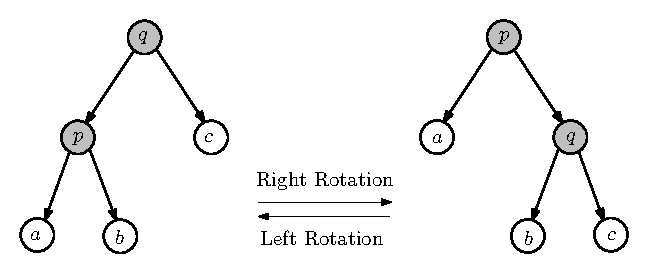
\includegraphics[width=6cm]{figs/treerotation}
\caption{\label{fig:treerotation}Left and right rotations of a BST.}
\end{center}
\end{figure}

\end{Example}

The precise details of exactly when a rotation is required, and which kind, 
differ depending on the type of balanced BST. In each case the programming of
the insertion and removal operations is quite complex, as is the analysis. 
We will not go into more details here---the reader should consult the  
recommended references.

Balancing of AVL trees requires extra memory and heavy
computations. This is why even more relaxed efficient balanced search
trees such as red-black trees are more often used in practice.

\begin{Definition}
A \defnfont{red-black tree} is a binary search tree such that 
every node is coloured either red or black, and every non-leaf node 
has two children. In addition, it satisfies the following properties: 
\begin{itemize}
\item the root is black;
\item all children of a red node must be black;
\item every path from the root node to a leaf must contain the same number of 
black nodes.
\end{itemize}
\end{Definition}

\begin{Theorem}
If every path from the root to a leaf contains $b$ black 
nodes, then the tree contains at least $2^{b}-1$ black nodes.
\end{Theorem}
\begin{proof}

The statement holds for $b=1$ (in this case
the tree contains either the black root only or the black
root and one or two red children). In line with the induction hypothesis, 
let the statement hold for all red-black trees with $b$ black nodes  in every 
path. If a tree contains $b+1$ black nodes in every path and has two black 
children of the root, then the tree contains two subtrees with $b$ black nodes 
just under the root and has in total at least 1+$2 \cdot(2^{b}-1) = 2^{b+1}-1$ 
black nodes. If the root has a red child, the latter has only black children, 
so that the total number of the black nodes can become even larger. 
\end{proof}

Each path cannot contain two consecutive red nodes and increase more
than twice after all the red nodes are inserted. Therefore, the height
of a red-black tree is at most $2\lceil \lg n \rceil$, and the
search in it is logarithmic, $O(\log n)$.

Red-black trees allow for a very fast search. This data structure has
still no precise analysis of its average-case performance. Its
properties are found either experimentally or by analysing red-black
trees containing random $n$ keys. There are about $\lg n$ comparisons per search 
on the average and fewer than $2\lg n + 2$ comparisons in the
worst case. Restoring the tree after insertion or deletion of single node 
requires $O(1)$ rotations and $O(\log n)$ colour changes in the worst case.

Another variety of balanced tree, the \defnfont{AA-tree}, becomes more efficient 
than a red-black tree when node deletions are frequent. An AA-tree has 
only one extra condition with respect to a red-black tree, namely that 
the left child may not be red. This property simplifies the removal 
operation considerably.

\subsection{Balanced B-trees: efficiency of external search}
\label{ss:B-tree}

The B-tree is a popular
structure for ordered databases in external memory such as magnetic or
optical disks. The previous ``Big-Oh'' analysis is invalid here because
it assumes all elementary operations have equal time complexity. This
does not hold for disk input / output where one disk access corresponds
to hundreds of thousands of computer instructions and the number of
accesses dominates running time. For a large database of many millions
of records, even logarithmic worst-case performance of red-black or
AA-trees is unacceptable. Each search should involve a very small number
of disk accesses, say, 3--4, even at the expense of reasonably
complex computations (which will still take only a small fraction of a disk access time).

Binary tree search cannot solve the problem because even 
an optimal tree has height $\lg n$. To decrease the
height, each node must have more branches. The height of an
optimal $m$-ary search tree ($m$-way branching) is roughly
$\log_{m} n$ (see Table~\ref{tbl:m-ary:branch}), or  
$\lg m$ times smaller than with an optimal binary tree 
(for example, $6.6$ times for $m=100$).

\begin{table}[htb!]
\caption{\label{tbl:m-ary:branch}Height of the optimal $m$-ary 
search tree with $n$ nodes.}
\centerline{
\begin{tabular}{|c|r|r|r|r|r|} \hline 
$n$ & $10^{5}$ & $10^{6}$ & $10^{7}$ & $10^{8}$  & $10^{9}$ \\ \hline
$\lceil \log_{2}n \rceil$  & 17  & 20  & 24  & 27  & 30 \\ \hline 
$\lceil \log_{10}n \rceil$ & 5   & 6   & 7   & 8   & 9 \\ \hline 
$\lceil \log_{100}n \rceil$ & 3   & 3   & 4   & 4   & 5 \\ \hline
$\lceil \log_{1000}n \rceil$ & 2   & 2   & 3   & 3   & 3 \\ \hline
\end{tabular}}
\end{table}

\begin{figure}[htb]
\begin{center}
\illustr{mtr-ex.ps}{90mm}
\caption{\label{mtr-ex} Multiway search tree of order $m=4$.}
\end{center}
\end{figure}

Figure~\ref{mtr-ex} shows that the search and the traversal of a
multiway search tree generalize in a straightforward way the binary
search tree operations. If in the latter case the search key is compared
to a single key in a node in order to choose one of two branches or stop
in the node, in an $m$-ary tree, the search key is compared to at most
$m-1$ keys in a node to choose one of $m$ branches. The major difference
is that multiple data records are now associated only with leaves
although some multiway trees do not strictly follow this condition. Thus
the worst-case and the average-case search involve the tree height and
the average leaf height, respectively.

\begin{Example}
Search for a desired key $k$ in Figure~\ref{mtr-ex} is guided by
thresholds, for example at the root it goes left if $k<4$, down if $4
\le k < 10$, and right if $k \ge 10$. The analogous comparisons are
repeated at every node until the record with the key $k$ is found at a
leaf or its absence is detected. Let $k=17$. First, the search goes
right from the root (as $17 > 10$), then goes to the third child of the
right internal node (as $17 \le 17 < 20$), and finally finds the desired
record in that leaf.
\end{Example}

\begin{Definition}
A \defnfont{B-tree} of order $m$ is an $m$-ary tree such that:
\begin{itemize} 
\item the root is either a leaf or it has between $2$ and
$m$ children inclusive; 
\item each nonleaf node (except possibly the root) has
between $\lceil m/2 \rceil$ and $m$ children inclusive;
\item each nonleaf node with $\mu$ children has $\mu-1$
keys, $(\theta[i]: i=1,\ldots,\mu-1)$, to guide the search where $\theta[i]$ is the smallest key in subtree $i+1$;
\item all leaves are at the same depth;
\item data items are stored in leaves, each storing between $\lceil l/2 \rceil$ and $l$ items, for some $l$.
\end{itemize} 
\end{Definition}

Other definitions of B-trees (mostly with minor changes) also exist, but
the above one is most popular. The first three conditions specify the
memory space each node needs (first of all, for $m$ links and $m-1$
keys) and ensure that more than half of it, except possibly in the root,
will be used. The last two conditions form a well-balanced tree.

\begin{figure}[htb]
\begin{center}
\illustr{mtr-b4.ps}{90mm}
\caption[2--4 B-tree with the leaf storage size 7.]%
{2--4 B-tree with the leaf storage size 7
($2..4$ children per node and $4..7$ data items per leaf).}
\label{mtr-b4} 
\end{center}
\end{figure}

\begin{note}
B-trees are usually named by their \defnfont{branching limits}, 
that is, $\lceil m/2 \rceil$--$m$, so that $2$--$3$ and $6$--$11$ 
trees are B-trees with
$m=3$ and $m=11$, respectively.
\end{note}

\begin{Example} In a
$2-4$ B-tree in Figure~\ref{mtr-b4} 
all nonleaf nodes have between 
$\lceil 4/2 \rceil = 2$ and $4$ children and thus from
$1$ to $3$ keys. The number $l$ of 
data records associated with a leaf depends on 
the capacity of external memory and the record size. 
In Figure~\ref{mtr-b4}, $l=7$ and each leaf stores between 
$\lceil 7/2 \rceil = 4$ and $7$  data items.
\end{Example}

Because the nodes are at least half full, a  B-tree with $m \ge 8$
cannot be a simple binary or ternary tree. Simple ternary $2$--$3$ B-trees
with only two or three children per node are sometimes in use for
storing ordered symbol tables in internal computer RAM. But branching
limits for B-trees on external disks are considerably greater to make
one node fit in a unit data block on the disk. Then the number of nodes
examined (and hence the number of disk accesses) decreases $\lg m$
times or more compared with a binary tree search.

In each particular case, the tree order $m$ and the leaf capacity $l$ 
depend on the disk block size and the size of records to
store. Let one disk block hold $d$ bytes, each key be of
$\kappa$ bytes, each branch address be of \(b\) bytes, 
and the database contain $s$ records, each of size $r$ bytes.
In a B-tree of order $m$, each nonleaf node stores at most $m-1$ keys 
and $m$ branch addresses, that is,
in total, $\kappa(m-1)+bm = (\kappa + b) m -\kappa$ bytes. 
The largest order $m$
such that one node fits in one disk block,
$(\kappa+b)m -\kappa \le d$, is 
$m=\left\lfloor \frac{d+\kappa}{b+\kappa}\right\rfloor$.
Each internal node, except the root,
has at least $\left\lceil \frac{m}{2} \right\rceil$ branches.
At most $l=\frac{d}{r}$ records fit in one block, and
each leaf addresses from $\frac{l}{2}$ to $l$ records. 
Assuming each leaf is full, the total number of the
leaves is $n = \left\lceil \frac{s}{l} \right\rceil$, so that
in the worst case the leaves are at level 
$\lceil \log_{m/2} n\rceil +1$.

\begin{Example}\label{exm:btree}
Suppose the disk block is $d=2^{15}\equiv 32768$ bytes, 
the key size is $\kappa=2^{6}\equiv 64$ bytes, the branch 
address has \(b=8\) bytes, and the
database contains $s=2^{30}\cong 1.07\cdot 10^9$ records
of size $r=2^{10}\equiv 1024$ bytes each. Then
the B-tree order is 
$m=\lfloor \frac{32768+64}{8+64} \rfloor =
\lfloor \frac{32832}{72} \rfloor = 456$ so that each internal node, 
except the root, has at least 228 branches.
One block contains at most $l=\frac{32768}{1024}=32$ records,
and the number of leaves is at least 
$n = \left\lceil 2^{30}/32 \right\rceil = 2^{25}$. The
worst-case level of the leaves in this B-tree is 
$\lceil \log_{228} 2^{25}\rceil +1 = \lceil 3.19 \rceil +1 = 5$.
\end{Example}

Generally, a search in or an insertion into a B-tree of order $m$ with $n$
data records requires fewer than $\lceil \log_{m/2}n \rceil$ disk
accesses, and this number is practically constant if $m$ is sufficiently
big as shown in Table~\ref{tbl:m-ary:branch}. The running time becomes
even smaller if the root and the upper two tree levels are stored in
internal RAM and the slow disk accesses occur only for level 3 or
higher. The three-level B-tree with $m=456$ can handle up to $456^{3}$,
or $94,818,816$ entries. If in Example~\ref{exm:btree} each key uses
only \(\kappa=24\) bytes, then $m = 1024$, and the three-level tree can
handle over $10^9$ entries.

Data insertion into a B-tree is simple if the corresponding leaf is not
already full. A full leaf has to be split into two leaves, both having
the minimum number of data items, and the parent node should be updated.
If necessary, the splitting propagates up until it finds a parent that
need not be split or reaches the root. Only in the extremely rare case
that the root has to be split, the tree height increases and a new root
with two children (halves of the previous root) is created. Data
deletion is also simple until the leaf is empty and its neighbours must
be combined to form a full leaf. Although the programming is not simple, all
changes are well defined. Algorithm analysis, beyond the scope of this
book, shows that both data insertion,
deletion, and retrieval have only about $\log_{\frac{m}{2}} n$ disk
accesses in the worst case.

\subsection*{Exercises}

\begin{Exercise}\label{exr:redblack:example}
Draw two different red-black trees containing at most two black nodes 
along every path from the root to a leaf.
\end{Exercise}


\begin{Exercise}\label{exr:avl:example}
Draw two different AVL trees of size $n=7$ and compare
them to the complete binary tree of the same size. Is
the latter also an AVL tree?
\end{Exercise}



\begin{Exercise}\label{exr:aa:example}
Draw an AA-tree containing at most 2 black nodes 
along every path from a node to a leaf and differing from
the complete binary tree of order \(n=7\).
\end{Exercise}

\begin{Exercise}\label{exr:rotation}
Draw a binary search tree of minimum size such that a left rotation 
reduces the height of the tree.
\end{Exercise}
% ------^^^ inserted from book ^^^---------


\chapter{Lecture: Hashing}
% ------vvv inserted from book vvv---------
There are numerous ways to implement the table ADT. We have already seen 
that various search trees will do everything required, provided the keys are 
from some totally ordered set. If, say, the keys are dictionary words with the 
usual ordering, then it is not necessary to use any integer encoding---keys can 
be compared directly.

Suppose now that we have a very simple situation where the number of 
possible keys is small. Then  we can just store the values in an array. 
One array entry can be reserved in advance for each possible key, and the 
key-to-value mapping ends up as a conventional array address. Searching then 
has worst-case constant time, as does insertion and deletion. This 
implementation of a table works well provided the number of possible keys is 
sufficiently small.

However, that nice state of affairs does not occur often (we could use it 
for the airport codes in  Example~\ref{exm:adt:airports}). Usually there exists 
a very large number of possible keys although only a tiny fraction of them are
actually put into use. For example, suppose that we have a database where each 
customer is identified by an 8-digit telephone number. If we have 10 000 customers, 
only $0.01\%$ of the array addresses are filled.

There is another technique to store and search for
values in symbol tables, called {\defnfont{hashing}}, that uses less space and 
retains many (not all) of the benefits of direct array addressing. 

\begin{Definition}
Hashing computes an integer \defnfont{hash code} for each object using a 
\defnfont{hash function} that maps objects (for example, keys) to indices of 
a given linear array (the \defnfont{hash table}). 
\end{Definition}

Hash functions are designed in such a manner that hash codes are
computed quickly. The computation  of an array index with 
a hash function, or ``hashing a key to an index'',
depends only on the key to hash and is independent of other keys in the table.
 If \(h(k)\) is the value of a hash function for $k$, then the
 key \(k\) should be placed at location \(h(k)\).

The hash function is chosen so as to always return a valid index 
for the array. A \defnfont{perfect hash function} maps each key to a different 
index. Unfortunately, it is difficult to find such a function in most cases. 

\begin{Example} \label{exm:hashing}
Let us map two-digit integer keys onto the ten array indices 
[0, 1, \ldots, 9] by a
simple hash function \(h(k) = \lfloor k/10 \rfloor\). Then the keys \(21\) and
\(27\) both have the hash code \(2\) pointing to
the same position in the array. Such a situation in which two different keys, 
\(k_{1} \ne k_{2}\), hash to the same index (table address), 
\(h(k_{1}) = h(k_{2})\), is called a \defnfont{collision}. Because both
table entries \((k_{1},v_{1})\) and \((k_{2},v_{2})\) cannot
be at the same address, we need a  definite {\defnfont{collision resolution policy}}. 
\end{Example}

Different keys hashed to the same hash address are  called \defnfont{synonyms}, 
and data items with synonymic keys are frequently also referred to as 
synonyms. 

\subsection{Collision resolution: OALP, OADH, and SC hash tables}

There are many collision resolution policies. The main issues are:

\begin{itemize}
\item Do we use extra storage, or not?
\item Which element moves when a collision occurs: the incumbent element or the 
newcomer (or both)?
\item How do we decide where to move the evicted element to?
\end{itemize}

\subsubsection{Chaining}

In \defnfont{separate chaining} synonyms with the same hash address are stored 
in a linked list connected to that address.  We still hash the key of 
each item to obtain an array index. But if there is a collision, 
the new item is simply placed in this hash address, along with all other
synonyms. Each array element is a head reference for the associated linked 
list, and each node of this list stores not only the key and data
values for a particular table entry but also a link to the
next node. The head node of the list referenced by the array
element always contains the last inserted item.

\subsubsection{Open addressing}

Open addressing uses no extra space for collision resolution. Instead, 
we move one of the colliding elements to another slot in the array. We may use
LIFO (last-in, first out --- the new element must move), FIFO (first in, first out 
--- the old element must move), or more complicated methods such as Robin Hood 
or cuckoo hashing (see Notes). For our purposes here, we use LIFO.

Each collision resolution policy \defnfont{probes} another array slot, and if 
empty inserts the currently homeless element. If the probed slot is not empty, we probe 
again to find a slot in which to insert the currently homeless element, and so on 
until we finish insertion. The \defnfont{probe sequence} used can be a simple 
fixed sequence, or given by a more complicated rule (but is always deterministic).
They all have the property that they ``wrap around" the array when they reach the 
end. The two most common probing methods are:
\begin{itemize}
\item (Linear probing) always probe the element to the left;
\item (Double hashing) probe to the left by an amount determined by the value of 
a secondary hash function.
\end{itemize}

\begin{note}
The choice of probing to the left versus probing to the right is clearly a 
matter of convention; the reader should note that other books may use rightward
probing in their definitions.
\end{note}

\begin{table}[hbt]
\begin{center}
\caption{Open addressing with linear probing (OALP).}\label{hash-lin} 
\begin{tabular}{|c|c|c|l|} \hline 
\textbf{Data} [key,value] & \textbf{Hash}: key/10 & \textbf{Table address} & \textbf{Comments} \\ \hline
~[20,A] & 2 & 2 & \\
~[15,B] & 1 & 1 & \\
~[45,C] & 4 & 4 & \\
~[87,D] & 8 & 8 & \\
~[39,E] & 3 & 3 & \\
~[31,F] & 3 & 0 & try 3, 2, 1, 0 \\
~[24,G] & 2 & 9 & try 2, 1, 0, 9 \\ \hline
\end{tabular}
\end{center}
\end{table}

\begin{Example}\label{exm:lin:probing}
Table~\ref{hash-lin} shows how OALP fills the hash table 
of size 10 using the two-digit keys and the hash function
of Example~\ref{exm:hashing}. The first five insertions have found
empty addresses. However, the key--value 
pair [31, F] has a collision because the address 
\(h(31) = 3\) is already occupied by the pair [39, E] with the same
hash address, \(h(39) = 3\). Thus, the 
next lower table address, location 2, is probed to see if
it is empty, and in the same way the next locations 1
and 0 are checked. The address 0 is empty so that the pair [31, F]
can be placed there. 

A similar collision occurs when we try to insert the next
pair, [24, G], because the hash address \(h(24)=2\) for
the key 24 is already occupied by the previous pair [20, A]. 
Consequently,  we probe successive lower locations 1 and 0, and 
since they both are already
occupied, we wrap around and continue the search at the highest
location 9. Because it is empty, the pair [24, G] is inserted in this location 
yielding the final configuration given in Table~\ref{hash-lin}.
\end{Example}

OALP is simple to implement but the hash table may degenerate due to
\defnfont{clustering}. A \defnfont{cluster} is a
sequence of adjacent occupied table entries. OALP tends to form clusters 
around the locations
where one or more collisions have occurred. Each
collision is resolved using the next empty location 
available for sequential probing. Therefore, other collisions 
become more probable in that neighbourhood, and the larger the
clusters, the faster they grow. As a result,
a search for an empty address to place a collided key may
turn into a very long sequential search. 

Another probing scheme, \defnfont{double hashing}, reduces the 
likelihood of clustering. In double hashing, when a collision occurs, the key
is moved by an amount determined by a secondary hash function \(\Delta\).  Let \(h\) denote
the primary hash function. Then for each key \(k\) we have the starting probe 
address \(i_{0} = h(k)\) and the probe decrement \(\Delta(k)\). Each
next successive probe position is 
\(i_{t} = ( i_{t-1} - \Delta(k) ) \bmod m\); \
\(t=1,2,\ldots\) where $m$ is the table size.

\begin{Example}\label{exm:double:hashing}
Table~\ref{hash-dbl} shows how OADH fills the same hash table as in
Example~\ref{exm:lin:probing} if the 
hash function is given by \(\Delta(k) = (h(k) + k) \bmod 10\).

\begin{table}[hbt]
\begin{center}
\caption{\label{hash-dbl} Open addressing with double hashing (OADH).}
\begin{tabular}{|c|c|c|l|} \hline 
\textbf{Data} [key,value] & \textbf{Hash}: key/10 & \textbf{Table address} & \textbf{Comments} \\ \hline
~[20,A] & 2 & 2 & \\
~[15,B] & 1 & 1 & \\
~[45,C] & 4 & 4 & \\
~[87,D] & 8 & 8 & \\
~[39,E] & 3 & 3 & \\
~[31,F] & 3 & 9 & using $\Delta(31)=4$ \\
~[24,G] & 2 & 6 & using $\Delta(24)=6$ \\ \hline
\end{tabular}
\end{center}
\end{table}

Now when we try to place the key--value 
pair [31, F] into position \(h(31) = 3\), the collision 
is resolved by probing the table locations with decrement
\(\Delta(31) = 4\). The first position, \((3-4)\mod 10 = 9\) is
empty so that the pair [31, F] can be placed there. 
For the collision of the pair, [24, G], at location 2 
the decrement \(\Delta(24) = 6\) immediately leads to
the empty location $6$. The final table
in Figure~\ref{hash-dbl} contains three small clusters 
instead of one large
cluster in Figure~\ref{hash-lin}. 
\end{Example}

Generally, OADH results in more uniform hashing that
forms more clusters than OALP but of smaller sizes.
Linear probing extends each cluster from its end with
the lower table address, and nearby clusters join into
larger clusters growing even faster. Double hashing does
not extend clusters only at one end and does not tend
to join nearby clusters.

% ------^^^ inserted from book ^^^---------

\chapter{Lecture: Analysis of Hashing}
% ------vvv inserted from book vvv---------
The time complexity of searching in and inserting items in a
hash table of size \(m\) with
\(n\) already occupied entries is determined by the \defnfont{load factor},
  \(\lambda := \frac{n}{m}\). In open addressing, \(0 \le \lambda < 1\): $\lambda$
  equals the fraction of occupied
slots in the array, and cannot be exactly equal to 1 because a hash table 
should have at least one empty entry in order to efficiently terminate the search 
for a key or the insertion of a new key.

Open addressing and separate chaining require $n$ probes in the worst case, 
since all elements of the hash table may be synonyms. However the basic intuition
is that provided the table is not too full, collisions should be rare enough that
searching for an element requires only a constant number of probes on average.

Thus we want a result such as: ``\emph{Provided the load factor is kept bounded 
(and away from 1 in the case of open addressing), all operations in a hash table 
take $\Theta(1)$ time in the average case.}"

In order to have confidence in this result, we need to describe our mathematical model of 
hashing. Since a good hash function should scatter keys randomly, and we have no
knowledge of the input data, it is natural to use the ``random balls in bins" 
model. We assume that we have thrown $n$ balls one at a time into $m$ bins, 
each ball independently and uniformly at random. 

For our analysis, it will be useful to use the function $Q$ defined below.
 
\begin{Definition}
For each integer $m, n$ with $1 \leq n \leq m$, we define 
$$
Q(m,n) = \frac{m!}{(m-n)! m^n} = \frac{m}{m} \frac{m-1}{m} \dots 
\frac{m - n + 1}{m}.
$$
Note that $Q(m,1) = 1$.
\end{Definition}

\subsubsection{Basic analysis of collisions}

It is obvious that if we have more items than the size of the hash table, at least 
one collision must occur. But the distinctive feature of collisions is that they 
are relatively frequent even in almost empty hash tables. 

The \defnfont{birthday paradox} refers to the following surprising fact:
\emph{if there are 23 or more people in a room, the chance is greater than 50\%
that two or more of them have the same birthday.} Note: this is not a paradox 
in the sense of a logical contradiction, but just a ``counter-intuitive" 
fact that violates ``common sense".

More precisely, if each of 365 bins
is selected with the same chance \(\frac{1}{365}\), then after
23 entries have been inserted, the probability that at least one collision has 
occurred (at least one bin has at least two balls) is more than 50\%. 
Although the table is only $23/365$ ($\cong 6.3\%$) full,
more than half of our attempts to insert one more entry will result in a collision!

Let us see how the birthday paradox occurs. Let \(m\) and \(n\) denote the 
size of a table and the number of items to insert, respectively. 
Let $\Pr_{m}(n)$ be the probability of at least one collision when 
$n$ balls are randomly placed into  $m$ bins.

\begin{Lemma}
The probability of no collisions when $n$ balls are thrown independently 
into $m$ boxes uniformly at random is $Q(m, n)$. Thus 
${\Pr_m}(n) =  1 - Q(m,n)$
and the expected number of balls thrown until the first collision is 
$\sum_{n\leq m} Q(m,n)$. 
\end{Lemma}

\begin{proof} Let $\pi_{m}(n)$ be the probability of no collisions.
 The ``no collision'' event after
inserting \(\nu\) items; \(\nu=2,\ldots,n\), is a joint event of
``no collision'' after inserting the preceding \(\nu-1\) items and 
``no collision'' after inserting one more item, given \(\nu-1\)
positions are already occupied. Thus 
\(\Pr_m(\nu)=\Pr_m(\nu-1)P_{m}(\mathrm{no~collision} \mid \nu-1)\)
where \(P_{m}(\mathrm{no~collision} \mid \nu)\) denotes the conditional
probability of no collision for a single item inserted into the
table with \(m-\nu\) unoccupied positions. This latter
probability is simply \(\frac{m-\nu}{m}\).

This then yields immediately
\[
\pi_{m}(n) = \frac{m}{m}\frac{m-1}{m} \dots \frac{m-n+1}{m} = 
\frac{m(m-1)\cdots(m-n+1)}{m^{n}} =  \frac{m!}{m^{n}(m-n)!}
\]
Therefore,
\(
\Pr_{m}(n) = 1 - \frac{m!}{m^{n}(m-n)!} = 1 - Q(m,n)
\)
which gives the first result.

The number of balls is at least $n+1$ with probability $Q(m,n)$. Since the 
expected value of a random variable $T$ taking on nonegative integer values 
 can always be computed by $E[T] = \sum_{n\geq 1} i \Pr(T=i) = 
 \sum_{j\geq 0} \Pr(T>j)$, and these latter probabilities are zero when $j>m$,
 the second result follows.
\end{proof}

Table~\ref{adt-tbl2} presents (to 4 decimal places)
some values of \(\Pr_{m}(n)\) for \(m=365\) and \(n=5\ldots100\). 
As soon as $m=47$ (the table with 365 positions is only 12.9\% full),
the probability of collision is greater than 0.95.
Thus collisions are frequent even in sparsely occupied tables.

\begin{table}[hbt!]
  \caption{\label{adt-tbl2} Birthday paradox: $\Pr_{365}(n)$.}
 \centerline{
  \begin{tabular}{|c|r|r|r|r|r|r|r|} \hline
    \(n\)          & 5 & 10 & 15 & 20 & 22  \\ \hline 
    \(\Pr_{365}(n)\) & 
       0.0271 & 0.1169 & 0.2529 & 0.4114 & 0.4757 \\
    \hline\hline 
    \(n\)          & 23 & 25 & 30 & 35 & 40  \\ \hline 
    \(\Pr_{365}(n)\) & 
       0.5073 & 0.5687 & 0.7063 & 0.8144 & 0.8912 \\
    \hline\hline 
    \(n\)          & 45 & 50 & 55 & 60 & 65  \\ \hline 
    \(\Pr_{365}(n)\) & 
       0.9410 & 0.9704 & 0.9863 & 0.9941 & 0.9977 \\
    \hline\hline 
    \(n\)          & 70 & 75 & 80 & 90 & 100  \\ \hline 
    \(\Pr_{365}(n)\) & 
       0.9992 & 0.9997 & 0.9999 & 1.0000 & 1.0000 \\
    \hline
  \end{tabular}}
\end{table}

Figure~\ref{fig:birthday} shows the graph of $\Pr_{365}(n)$ as a function of $n$.
The median of this distribution occurs around $n=23$, as we have said above, and
so 23 or more balls suffice for the probability of a collision to exceed 1/2. 
Also, the expected number of balls before the first collision is easily computed
to be 25. 

\begin{figure}
\begin{center}
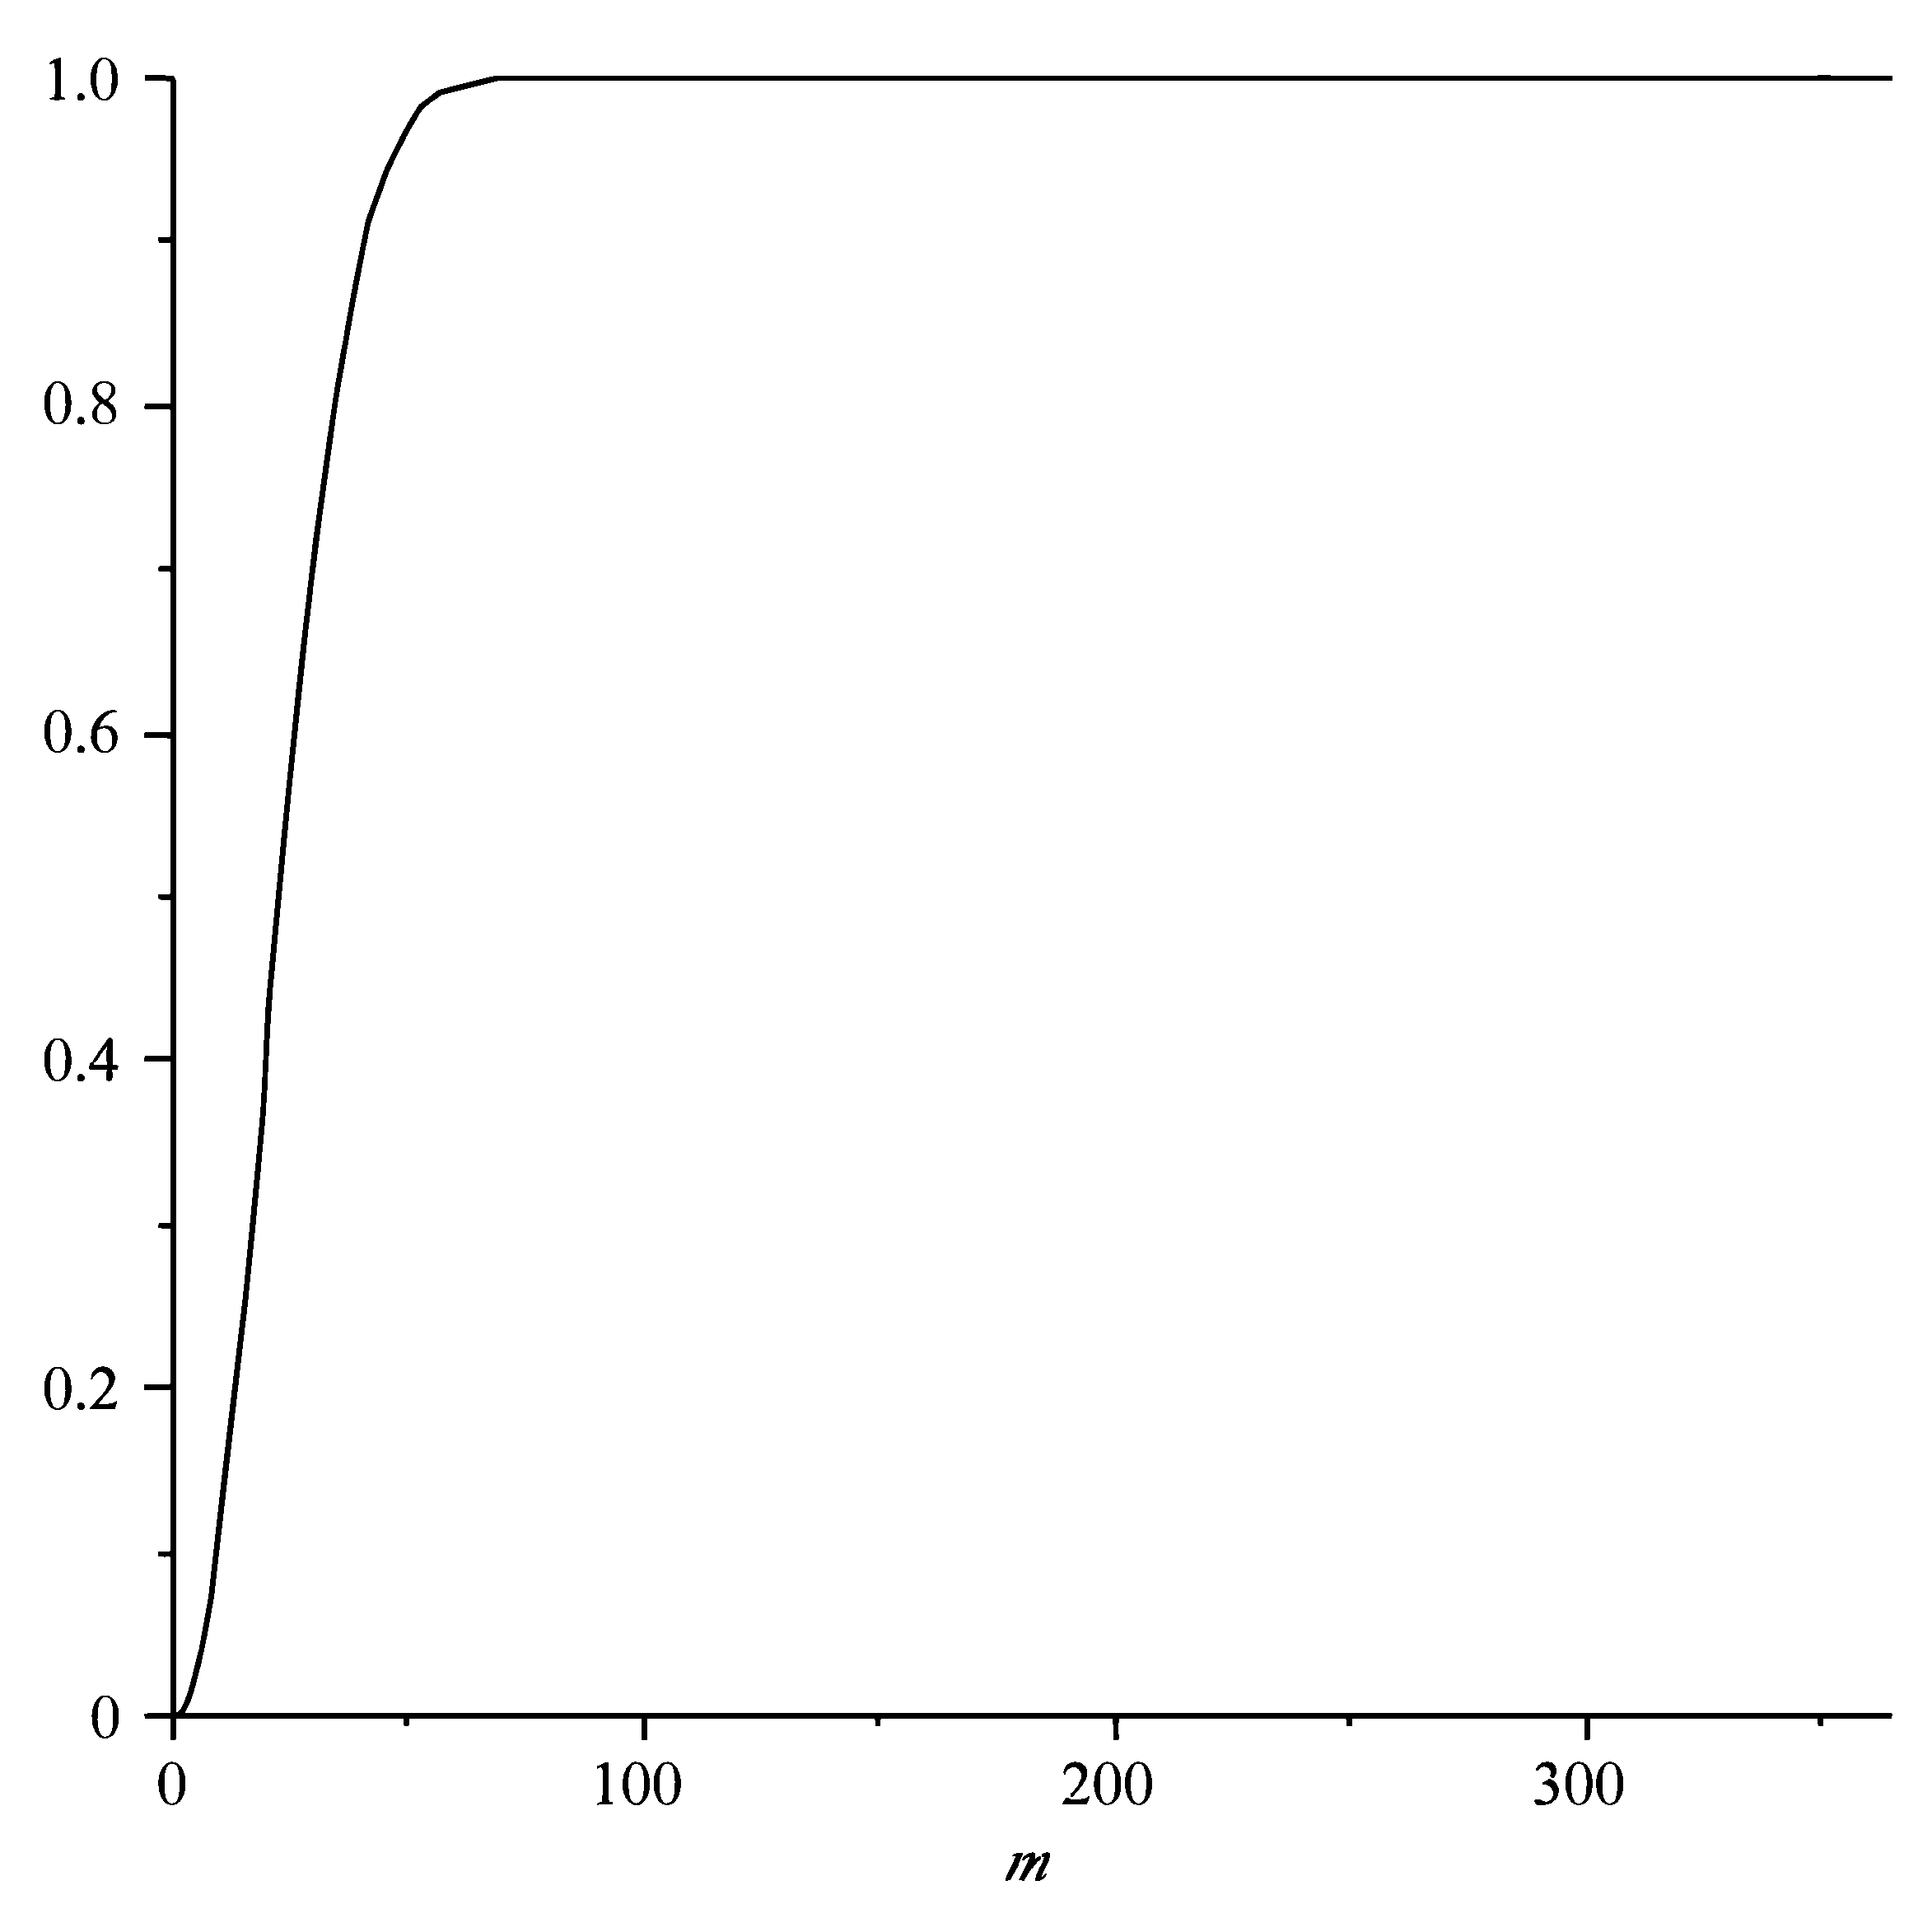
\includegraphics[width=6cm]{figs/birthday365.eps}
\end{center}
\caption{\label{fig:birthday} Birthday paradox: $\Pr_{365}(n)$.}
\end{figure}

When the load factor is much less than $1$, the average number of balls per bin
is small. If the load factor exceeds $1$ then the average number is large. In 
each case analysis is not too difficult. For hashing to be practical, we need 
to be able to fill a hash table as much as possible before we spend valuable 
time \defnfont{rehashing} --- that is, allocating more space for the table
 and reassigning hash codes via a new hash function. Thus we need to analyse 
 what happens when the load factor is comparable to $1$, that is, when the 
 number of balls is comparable to the number of bins. This also turns out to be
 the most interesting case mathematically.

\subsubsection{Theoretical analysis of hashing}

In addition to the basic operations for arrays, we also 
consider the computation of the hash address of an item to be an elementary 
operation.

Chaining is relatively simple to analyse. 

\begin{Lemma}\label{lem:sc}
The expected running time for unsuccessful search
in a hash table with load factor \(\lambda\) using
separate chaining is given by 
$$T_{\mathrm{us}}(\lambda)= 1+\lambda. $$
The expected running time for successful search is $O(1 + \lambda/2)$.

Update, retrieval, insertion and deletion all take time that is $O(1+\lambda)$.
\end{Lemma}
\begin{proof}
In an unsuccessful search for a key \(k\), the computation of
the hash address, \(h(k)\), takes one elementary
operation. The average running time to unsuccessfully search for the
key at that address is equal to the average length of the
associated chain, \(\lambda=\frac{n}{m}\). Thus in total
$T_{\mathrm{us}}(\lambda) = 1 + \lambda = 1 + n/m$.

The result for successful search and other operations 
now follows from Lemma~\ref{lem:ss-us}, since update, retrieval and deletion from a 
linked list take constant time.
\end{proof}

To analyse open addressing, we must make some extra assumptions. We use the 
\defnfont{uniform hashing hypothesis}: each configuration of $n$ keys in a 
hash table of size $m$ is equally likely to occur. This is what we would expect 
of a truly ``random" hash function, and it seems experimentally 
to be a good model for double hashing. Note that this is stronger than just 
requiring that each key is independently and uniformly likely to hash initially 
to each slot before collision resolution (``random balls in bins").
It also implies that all probe sequences are equally likely.

\begin{Lemma}\label{lem:oadh}
Assuming the uniform hashing hypothesis holds, 
the expected number of probes for search in a hash table satisfy
$$
T_{\mathrm{us}}(\lambda) \leq \frac{1}{1-\lambda} 
$$
and
$$ 
T_{\mathrm{ss}}(\lambda) \leq \frac{1}{\lambda} \ln \frac{1}{1-\lambda}.
$$
\end{Lemma}

\begin{proof} 
The average number of probes for an
unsuccessful search is
\(
T_{\mathrm{us}}(\lambda) = \sum_{i=1}^{n}i p_{m,n}(i)
\)
where \(p_{m,n}(i)\) denotes the probability of exactly \(i\)
probes during the search. Obviously, 
\(p_{m,n}(i) = \Pr (m,n,i) - \Pr (m,n,i+1)\) where 
\(\Pr (m,n,i)\) is the probability of \(i\) or more probes
in the search. By a similar argument to that used in the
birthday problem analysis we have for $i\geq 2$
$$
\Pr (m,n,i) = \frac{n}{m}\cdot \frac{n-1}{m-1} \cdots \frac{n-i+2}{m-i+2}
$$
while $\Pr (m,n,1) = 1$.
Note that clearly $\Pr (m,n,i) \leq (n/m)^{i-1} = \lambda^{i-1}.$
Thus
\begin{eqnarray*}
T_{\mathrm{us}}(\lambda) & = &
\sum\limits_{i=1}^{n}i\left ( 
{\textstyle \Pr (n,m,i) - \Pr (n,m,i+1) }\right ) \\
& \le &
\sum\limits_{i=1}^{\infty}i\left ( 
{\textstyle \Pr (n,m,i) - \Pr (n,m,i+1)}\right ) 
= \sum\limits_{i=1}^{\infty} \Pr (n,m,i) 
\le  
\sum\limits_{i=1}^{\infty} \lambda^{i-1} = \frac{1}{1-\lambda} = \frac{m}{m-n}.
\end{eqnarray*}

The result for successful search now follows by averaging. We have
\begin{align*}
T_{\mathrm{ss}}(\lambda) & \leq \frac{1}{n} \sum_{i=0}^{n-1} \frac{m}{m-i} \\
& = \frac{1}{\lambda} \sum_{j=m-n+1}^m \frac{1}{j}\\
& \leq \frac{1}{\lambda} \int_{n-m}^n dx/x = \frac{1}{\lambda} \ln\left(\frac{m}{m-n}\right) = \frac{1}{\lambda}
\ln\left(\frac{1}{1-\lambda}\right).
\end{align*}
\end{proof}

\begin{note}
It can be shown that the exact values are
\begin{align*}
T_{\mathrm{us}}(\lambda) & = \frac{m+1}{m-n+1} \approx \frac{1}{1-\lambda}\\
T_{\mathrm{ss}}(\lambda) & = \frac{m+1}{n} \left( H_{m+1} - H_{m-n+1} \right) 
\approx \frac{1}{\lambda} \ln\left(\frac{1}{1-\lambda}\right)
\end{align*}
so that the upper bounds in the theorem are asymptotically precise as $m\to \infty$.
\end{note}

Good implementations of OADH have been shown in theory and practice to be well 
described by the simple uniform hashing model above, so we may safely use the above
results. 

However, OALP is not well 
described by the uniform hashing model, because of its clustering 
behaviour. It can be analysed, however, in a similar but more complicated manner.

\begin{Lemma}\label{lem:oalp}Assuming uniformly hashed random input,
the expected number of probes for successful, $T_{\mathrm{ss}}(\lambda)$,
and unsuccessful, $T_{\mathrm{us}}(\lambda)$, search in a hash table using 
OALP are, respectively, 
\[
T_{\mathrm{ss}}(\lambda)\approx
0.5 \left ( 1 + \frac{1}{1-\lambda}\right ) 
\; \;\;\; 
\mathrm{and}
\; \;\;\; 
T_{\mathrm{us}}(\lambda)\approx
0.5 \left ( 1 + \left ( \frac{1}{1-\lambda} \right )^2 \right )
\]
\end{Lemma}
\begin{proof}
The proof is beyond the scope of this book (see Notes).
\end{proof}

The relationships in Lemma~\ref{lem:oalp} and Lemma~\ref{lem:oadh}
completely fail when \(\lambda=1\). But the latter situation indicates a full 
hash table, and we should avoid getting close to it anyway. 

Unlike OALP and OADH, the time estimates for separate chaining (SC) remain
valid with data removals. Because each chain may keep several 
table elements, the load factor may be more than $1$.

\begin{table}[htb!]
  \caption{\label{tbl-hash}Average search time bounds in hash tables with
           load factor $\lambda$.} 
 \centerline{
  \begin{tabular}{|c|ccc|ccc|} \hline
   \(\lambda\) & 
   \multicolumn{3}{c|}{Successful search: $T_{\mathrm{ss}}(\lambda)$} &
   \multicolumn{3}{c|}{Unsuccessful search: $T_{\mathrm{us}}(\lambda)$} 
   \\ \cline{2-7}
               & \textbf{SC} & \textbf{OALP} & \textbf{OADH} 
               & \textbf{SC} & \textbf{OALP} & \textbf{OADH}\\ \hline
0.10 & 1.05 & 1.06 & 1.05 & 1.10 & 1.12 & 1.11 \\
0.25 & 1.12 & 1.17 & 1.15 & 1.25 & 1.39 & 1.33 \\
0.50 & 1.25 & 1.50 & 1.39 & 1.50 & 2.50 & 2.0 \\
0.75 & 1.37 & 2.50 & 1.85 & 1.75 & 8.50 & 4.0 \\
0.90 & 1.45 & 5.50 & 2.56 & 1.90 & 50.5 & 10.0 \\
0.99 & 1.49 & 50.5 & 4.65 & 1.99 & 5000.0 & 100.0 \\ \hline
  \end{tabular}}
\end{table}

Table~\ref{tbl-hash} presents the above theoretical 
estimates of the search time in the OALP, OADH, and SC hash tables under 
different load factors. Average time measurements for actual hash
tables~\cite{standish} are close to the estimates for SC tables in  the whole
range \(\lambda \le 0.99\) and seem to be valid for larger
values of \(\lambda\), too. The measurements for OADH tables
remain also close to the estimates up to  \(\lambda = 0.99\).
But for OALP tables, the measured time is considerably
less than the estimates if \( \lambda > 0.90\) for a successful search and 
\( \lambda > 0.75\) for an unsuccessful search.

\begin{Example}
The expected performance of hashing depends only on the load factor.
If \(\lambda = 0.9\), OADH 
double hashing takes on the average 2.56 and 10 probes for 
successful and unsuccessful search, respectively. But 
if \(\lambda = 0.5\), that is, the same keys are stored 
in a roughly twice larger table, the same numbers decrease
to 1.39 and 2 probes.
\end{Example}


\subsection{Implementation of hashing}

\subsubsection{Resizing} 
One problem with open addressing is that successive insertions may cause the table
to become almost full, which degrades performance. Eventually we will need to 
increase the table size. Doing this each time an element is inserted is very 
inefficient. It is better to use an upper bound, say $0.75$, on the load factor, 
and to double the array size when this threshold is exceeded. This will then require 
recomputing the addresses of each element using a new hash function.

The total time required to resize, when growing a table from $0$ to $m=2^k$ elements,
is of order $1 + 2 + 4 + 8 + \dots + 2^{k-1} = 2^k - 1 = m - 1$. Since the $m$ 
insertions take time of order $m$ (recall the table always has load factor 
bounded away from $1$), the average insertion time is still $\Theta(1)$.

\subsubsection{Deletion}

It is quite easy to delete a table entry from a hash table with separate 
chaining (by mere node deletion from a linked list). However, open addressing 
encounters difficulties. If a particular table entry is physically removed
from a OA-hash table leaving an empty entry in that place, the search for 
subsequent keys becomes invalid. This is because the OA-search terminates when 
the probe sequence encounters an empty table entry. Thus if a previously occupied 
entry is emptied, all probe sequences that 
previously travelled through that entry will
now terminate before reaching the right location. 

To avoid this problem, the deleted entry is normally marked in such a way that
insertion and search operations can treat it as an empty and 
nonempty location, respectively. Unfortunately, such a policy results in hash 
tables packed with entries which are marked as deleted. But in this case the 
table entries can be rehashed to preserve only actual data and really delete all
marked entries. In any case, the time to delete a table entry remains \(O(1)\) 
both for SC  and OA hash tables.

\subsubsection{Choosing a hash function}
\label{sec:choice:hash:fun} 

Ideally, the hash 
function, \(h(k)\), has to map keys uniformly and randomly onto 
the entire range of hash table addresses. Therefore, the
choice of this function has much in common with the choice of
a generator of uniformly distributed pseudorandom numbers. 
A randomly chosen key \(k\) has to equiprobably hash to each
address so that uniformly distributed keys produce uniformly
distributed indices \(h(k)\). A poorly designed hash function
distributes table addresses nonuniformly and tends to
cluster indices for contiguous clusters of keys. 
A well designed function scatters the keys as to avoid
their clustering as much as possible.

If a set of keys is fixed, there always exists a \defnfont{perfect hash function}
that maps the set one-to-one onto a set of table indices and thus entirely 
excludes collisions. However, the problem is how to design such a function as
it should be computed quickly but without using large tables.
There exist techniques to design perfect hash functions for given sets of keys. 
But perfect hashing is of very limited interest because in most applications 
data sets are not static and the sets of keys cannot be pre-determined.

Four basic methods for choosing a hash function
are \defnfont{division}, \defnfont{folding}, \defnfont{middle-squaring}, and 
\defnfont{truncation}.
\begin{description}
\item[Division] assuming the table size is a prime number \(m\) 
and keys, \(k\), are integers,
the quotient, \(q(k,m)=\left \lfloor \frac{k}{m} \right \rfloor \), 
and the remainder, \(r(k,m)=k \mod m\), of the integer division of
\(k\) by \(m\) specify the
probe decrement for double hashing and the value
of the hash function \(h(k)\), respectively:
$$
h(k) = r(k,m) \mbox{ and }
\Delta(k) = \max \left \{
1, \ q(k,m) \bmod m \right\} \quad . 
$$
The probe decrement is put to the range \([1,\ldots,m-1]\) because all
decrements should be nonzero and point to the indices
\([0,1,\ldots,m-1]\) of the table. The reason that $m$ should be prime is that 
otherwise some slots may be unreachable by a probe sequence: for example if 
$m=12$ and $\Delta(k) = 16$, only $3$ slots will be probed before the sequence
returns to the starting position.

\item[Folding] an integer key \(k\) is divided into sections and 
the value \(h(k)\) combines sums, differences, and products of
the sections (for example, a 9-digit decimal key, such as 
\(k=013402122\), can be split into three sections:
013, 402, and 122, to be added together for getting 
the value \(h(k)=537\) in the range \([0,\ldots,2997]\)).

\item[Middle-squaring] a middle section of an integer key
\(k\), is selected and squared, then a middle section of 
the result is the value \(h(k)\) (for example, the squared middle section, 402, of 
the above 9-digit key, \(k=013402122\), results in 161604, and
the middle four digits give the value \(h(k)=6160\) in the range
\([0,\ldots,9999]\)).

\item[Truncation] parts of a key are simply cut out and 
the remaining digits, or bits, or characters are used
as the value \(h(k)\)  
(for example, deletion of all but last three digits 
in the above 9-digit key, \(k=013402122\),
gives  
the value \(h(k)=122\) in the range \([0,\ldots,999]\)).
While truncation is extremely fast, the keys do not scatter
randomly and uniformly over the hash table indices. This is
why truncation is used together with other methods, but 
rarely by itself.
\end{description}

Many real-world hash functions combine some of the above methods.
                                            
We conclude by discussing the idea of \emph{universal hashing}. We have seen 
(in the section on quicksort) the idea of using randomization to 
protect against bad worst-case behaviour. An analogous idea works for hashing.
                                           
If a hash table is dynamically changing and its elements 
are not known in advance, any fixed hash function can result in 
very poor performance on certain inputs, because of collisions. 
Universal hashing allows us to reduce the probability of this occurrence
by randomly selecting the hash function at run time from a large set
of such functions. Each selected function still may be bad for a
particular input, but with a low probability
which remains equally low if the same input is met once again.
Due to its internal randomisation, universal hashing behaves well even for
totally nonrandom inputs. 

\begin{Definition}
Let \(K\), \(m\), and \(F\) denote
a set of keys, a size of a hash table (the range of indices),
and a set of hash functions mapping \(K\) to \(\{0,\ldots,m-1\}\),
respectively. Then \(F\) is a \defnfont{universal class} if any
distinct pair of keys \(k,\kappa \in {K}\)  collide
for no more than \(\frac{1}{m}\) of the functions in the class \({F}\),
that is,
\[
\frac{1}{|{F}|}
\left| \raisebox{10pt}{} \left\{ h \in {F} \mid \ h(k) = h(\kappa)\right\}\right|
\le \frac{1}{m} \quad .
\]
%where \(|Z|\) denotes cardinality of a finite
%set \({Z}\).

\end{Definition}
Thus in the universal class all key pairs behave well and the
random selection of a function from the class results in a probability of at most
\(\frac{1}{m}\) that any pair collide.

One popular universal class of hashing functions is produced by
a simple division method. It assumes the keys are integers and
cardinality of
the set of keys \({K}\) is a prime number larger 
than the largest actual key. The size \(m\) of the hash
table can be arbitrary. This universal class is described by
the next theorem.

\begin{Theorem}[Universal Class of Hash Functions] 
\label{the:ucf}
Let \({K}=\{0,\ldots,p-1\}\) and \(|{K}| = p\) be
a prime number. 
For any pair of integers \(a \in \{1, \ldots, p-1\}\)
and \(b \in \{0, \ldots, p-1\}\), let
\(
h_{a,b}(k) = \left ( (ak + b) \bmod p \right ) \bmod m
\).
Then
\[
{F} = \{h_{a,b} \mid \ 1 \le a < p \;\; \mathrm{and} \;\; 0 \le b < p \}
\]
is a universal class.
\end{Theorem}
\begin{proof}
It is easily shown that the number of collisions in the
class \({F}\), 
\[
\left| \raisebox{10pt}{} \{h\in {F} \mid  h(k)= h(\kappa); \ k,\kappa\in {K}\}\right|,
\]
is the number of distinct numbers \((x,y)\);
\(0 \le x,y < p\) such that 
\(x \bmod m = y \bmod m\). Let us denote the latter property: 
\(x \equiv y \pmod m\). %; (\hspace*{-3mm}\mod n)\).
It is evident that \(h_{a,b}(k) = h_{a,b}(\kappa)\) iff 
\[
(ak + b ) \bmod p  \equiv 
(a\kappa + b ) \bmod p  \pmod m \quad .
\]

Then for any fixed \(k, \kappa < p\), there is one-to-one
correspondence between the pairs \((a,b)\) such that
\(0 < a < p\) and \(0 < b < p\) and \(h_{a,b}(k) = h_{a,b}(\kappa)\),
and the pairs of distinct numbers \((x,y)\) with the
property that \(0 \le x,y < p\) and \(x \equiv y \pmod n\).
The correspondence is given in one direction by
\[
x = (ak + b) \bmod p; \;\; y = (a\kappa + b) \bmod p
\]
where \(x \ne y\) since 
\[
\{ az + b \mid \ z = 0, \ldots, p-1\} = \{0, \ldots, p-1\}
\]
when \(p\) is prime and \(a \ne 0\). In the other direction
the correspondence is given by the condition that \(a\) and
\(b\) are the unique integers in \(\{0, \ldots, p-1\}\) such
that
\[
ak + b \equiv x \pmod p \; \;\;\mathrm{and}\;\;\;
a\kappa + b \equiv y \pmod p \quad .
\]
These equations have a unique solution for \(a\) and \(b\)
since \(p\) is prime, and \(a \ne 0\) since \(x \ne y\).

Clearly \(|{F}| = p(p-1)\). Now let us find out how many 
pairs of distinct numbers
\((x,y)\) exist such that \(0 \le x,y < p\) and 
\(x \equiv y \pmod m\). For any fixed \(s < m\) there are
at most \( \left \lceil \frac{p}{m} \right \rceil \) numbers
\(x < p\) such that \(x \equiv s \pmod m\). Since \(p\) and
\(m\) are integers,
\(
\left \lceil \frac{p}{m} \right \rceil \le \frac{p-1}{m} +1
\).
Therefore for each \(x < p\) there are no more than
\(\frac{p}{m} -1 \le \frac{p-1}{m}\) numbers \(y < p\)
distinct from \(x\) such that \(x \equiv y \pmod m\), and
the total number of such pairs \((x,y)\) is at most 
\(\frac{p(p-1)}{m}\). Hence for any fixed distinct
pair of keys \((k,\kappa)\) the fraction of \({F}\)
that cause \(k\) and \(\kappa\) to collide is at
most \(\frac{1}{m}\), so the class \({F}\) is universal.
\end{proof}

This suggests the following strategy for 
choosing a hash function at run time: (i) find 
the current size of the set of keys to hash; 
(ii) select the next 
prime number \(p\) larger than the size of the key set found;
({iii}) randomly choose integers \(a\) and \(b\)
such that \(0 < a < p\) and \(0 \le b < p\), and 
({iv}) use the function \(h_{a,b}\) 
defined in Theorem~\ref{the:ucf}.


\subsection*{Exercises}

\begin{Exercise}\label{exr:java:hash}
The Java programming language (as of time of writing)
uses the following hash function $h$ for character strings. 
Each character has a Unicode value represented by an integer (for example, the 
upper case letters $A, B, \dots, Z$ correspond to $65, 66, \dots, 90$ and the 
lower case $a, b, \dots, z$ correspond to $97, 98, \dots, 122$). Then 
$h$ is computed using 32-bit integer addition via
$$h(s) = s[0]*31^{n-1} + s[1]*31^{n-2} + \dots + s[n-1]*31 + s[n].$$

Find two 2-letter strings that have the same hash value. How could you use this 
to make $2^{100}$ different strings all of which have the same hash code?
\end{Exercise}

\begin{Exercise}\label{exr:hash:oalp}
Place the sequence of keys \(k=10, 26, 52, 76, 13, 8, 3, 33, 60, 42\) 
into a hash table of size 13 using the modulo-based hash address \(i = k \mod 13\) 
and linear probing to resolve collisions.
\end{Exercise}

\begin{Exercise}\label{exr:hash:oadh}

Place the sequence of keys \(k=10, 26, 52, 76, 13, 8, 3, 33, 60, 42\) 
into a hash table of size 13 using the modulo-based hash address \(i = k \mod 13\) 
and double hashing with the secondary hash function 
\(\Delta(k)=\max\{1, k/13 \}\) to resolve collisions.
\end{Exercise}

\begin{Exercise}\label{exr:hash:sc}
Place the sequence of keys \(k=10, 26, 52, 76, 13, 8, 3, 33, 60, 42\) 
into a hash table of size 13 using separate chaining to resolve collisions.
\end{Exercise}
% ------^^^ inserted from book ^^^---------

\chapter{Lecture: Universal Hashing}

%\part{Introduction to Graph Algorithms}

\part{The Graph Abstract Data Type}
\label{ch:graphadt} 

\chapter{Graph definitions} %-------------------------------------------------
\label{sec:graphdefs}
Graphs are important and general mathematical objects that are widely used in theory and practice. 
They distill the basic idea of a relationship among a set of objects. 
Informally we can think of a graph as a collection of dots (the set of objects) with lines connecting them (describing the relationship). 
The lines can be either directed (arrows) or undirected.

We are interested in the algorithmic aspects of graph theory (``how can we do it efficiently and systematically?").  
To talk about this precisely, we must start with precise definitions.

\begin{Definition}\label{def:digraph} 
A \defnfont{digraph} $G=(V,E)$ is a  finite nonempty set $V$ of \defnfont{nodes} 
together with a (possibly empty) set $E$ of ordered pairs of nodes of $G$ called \defnfont{arcs}. 
Digraph stands for \boldfont{di}rected \boldfont{graph}.
\end{Definition}

\begin{Boxample}[0] \label{ex:digraph}
For the digraph shown below, write down the sets $V$ and $E$.\\
\newline 
\includegraphics{graphExDirectedVE}
\end{Boxample}

\begin{Definition}\label{def:graph}
A \defnfont{graph} $G = (V, E)$ is a finite nonempty  set $V$ of 
\defnfont{vertices} together with a (possibly empty) set $E$ of unordered
pairs of vertices of $G$ called \defnfont{edges}. 
Note that the singular of vertices is \defnfont{vertex}.
\end{Definition}

\begin{Boxample}[0] \label{ex:graph}
For the graph shown below, write down the sets $V$ and $E$.\\
\newline 
\includegraphics{graphExUndirectedVE}
\end{Boxample}

Some notes on graphs vs digraphs.
\begin{itemize}
  \item In order to save writing ``(di)graph" too many times, we treat the digraph as the fundamental concept.
  \item When we say something about digraphs, nodes and arcs, it is understood to also hold for graphs, 
  vertices and edges unless explicitly stated otherwise. 
  \item However, if we talk about graphs, vertices and edges, our statement is not necessarily true for digraphs. 
  \item Some authors use ``undirected graph'' to mean graph and use the term ``graph" to mean what we call a directed graph. 
  We always use digraph and graph.
  \item $E$ is a set so there are no multiple arcs between a pair of nodes.
  \item An arc that begins and ends at the same node is called a \defnfont{loop}. 
  We make the convention that \boldfont{loops are not allowed in our digraphs}. 
  \item For a digraph $G$ we may denote the node set $V(G)$ and arc set $E(G)$ for clarity.
  \item A graph can be viewed as a digraph where every unordered edge $\{u, v\}$ 
  is replaced by two directed arcs $(u, v)$ and $(v, u)$.  
  This works in most instances and has the advantage of allowing us to consider only digraphs.
%  \item Sometimes we must know whether our object is really a graph or just a symmetric digraph. Whenever there
%  is a potential ambiguity, we shall point it out.
\end{itemize}

\begin{Definition}\label{def:adjacent}  
If $(u, v)\in E$ (that is, if there is an arc going from $u$ to $v$) we say that $v$ is \defnfont{adjacent} 
to $u$, that $v$ is an \defnfont{out-neighbour} of $u$, and that $u$ is an \defnfont{in-neighbour} of $v$.
In an (undirected) graph $G$, if $\{u, v\} \in E$, then $u$ is a \defnfont{neighbour} of $v$ and $v$ is a neighbour of $u$. 
\end{Definition}

\begin{Boxample}[2]
In the digraph in \cref{ex:digraph}, find all in-neighbours of node 2 and all out-neighbours of node 0.
\end{Boxample}

\begin{Definition} 
The \defnfont{order} of a digraph $G = (V, E)$ is $\abs{V}$, the number of nodes. 
The \defnfont{size} of $G$ is $\abs{E}$, the number of arcs. 
We usually use $n$ to denote $\abs{V}$ and $m$ to denote $\abs{E}$.
\end{Definition}
 
For a given order $n$, the size $m$ can be as low as $0$ (a digraph consisting of $n$ nodes and no arcs)  
and as high as $n(n-1)$ (each node can point to each other node; recall that we do not allow loops).

\begin{Definition}  
If $m$ is toward the low end, the digraph is called \defnfont{sparse}, 
and if $m$ is toward the high end, then the digraph is called \defnfont{dense}. 
These terms are obviously very informal. 
For our purposes we will call a class of digraphs sparse if $m$ is $O(n)$ and dense if $m$ is $\Omega(n^2)$.
\end{Definition}

\begin{Definition} 
A \defnfont{walk} in a digraph $G$ is a sequence of nodes $v_0\, v_1\, \ldots\, v_l$ 
such that, for each $i$ with $0 \leq i < l$, $(v_i, v_{i+1})$ is an arc in $G$. 

The \defnfont{length} of the walk $v_0\, v_1\, \ldots \,v_l$ is the number $l$ (that is, the number of arcs involved).

A \defnfont{path} is a walk in which no node is repeated. 

A \defnfont{cycle} is a walk in which $v_0 = v_l$ and no other nodes
are repeated.
\end{Definition}

In a graph, a walk of the form $u\, v\, u$ -- going back and forth along the same edge -- is not considered a cycle. 
A cycle in a graph must be of length at least $3$.
Note that a walk and a path can have length 0.


\begin{Boxample}
For the graph on the left the following
sequences of vertices are classified as being walks, paths, or cycles. Complete the table.\\

\begin{minipage}[c]{0.3\textwidth}
\centering
\includegraphics{graphExUndirected}
\end{minipage}
\begin{minipage}[c]{0.65\textwidth}
\begin{tabular}{|l|c|c|c|}\hline
\textbf{vertex sequence} & \textbf{walk?} & \textbf{path?} & \textbf{cycle?} \\ \hline
$0\, 3\, 2$                  & no  & no  &   \\
$0\, 1\, 2\, 3\, 4$          &     & yes & no  \\
$0\, 1\,  2\,  0$            & yes &     & yes  \\
$0 \, 1\,  0$                & yes & no  &  \\
$1\,  2\,  3\,  4\,  2\,  0$ &     &     &  \\
$3$							 & yes &     &  \\
\hline
\end{tabular}
\end{minipage}
\end{Boxample}

\begin{Boxample}[7]
Show that if there is a walk from $u$ to $v$, then we can find a path from $u$ to $v$.
\end{Boxample}

\begin{Definition} 
In a graph, the \defnfont{degree} of a vertex $v$ is the number of edges meeting $v$. 
In a digraph, the \defnfont{outdegree} of a node $v$ is the number of out-neighbours of $v$, 
and the \defnfont{indegree} of $v$ is the number of in-neighbours of $v$.

A node of indegree $0$ is called a \defnfont{source} and a node of outdegree $0$ is called a \defnfont{sink}.
\end{Definition}

%\begin{Boxample}[3]
%Prove that in a digraph, the sum of all outdegrees equals the sum of all 
%indegrees. What is the analogous statement for a graph? 
%\end{Boxample}

\begin{Definition}
The \defnfont{distance} from $u$ to $v$ in $G$, denoted by $d(u,v)$, is 
the number of arc on a shortest path from $u$ to $v$. If no path from $u$ to $v$ exists, the 
distance is undefined (or $+\infty$).
\end{Definition}

For graphs, we have $d(u,v) = d(v,u)$ for all vertices $u, v$. 

\begin{Boxample}[2]
Give the following distances for the digraph on the left.\\
\newline
\includegraphics{distancesDirected}
\newline

Why are the values $d(4, v)$ not defined unless $v = 4$?
\end{Boxample}

\section{Creating new digraphs from old ones}
There are several ways to create new digraphs from old ones.
One way is to delete nodes and arcs in such a way that the 
resulting object is still a digraph (no arcs missing endpoints).

\begin{Definition}
A \defnfont{subdigraph} of a digraph $G = (V, E)$ is a digraph $G' = (V', E')$ 
where $V'\subseteq V$ and $E'\subseteq E$. 
A \defnfont{spanning} subdigraph is one with $V' = V$; that is, it contains all nodes.
\end{Definition}

\begin{Boxample}
A digraph (left) with a subdigraph (middle) and a spanning subdigraph (right).
\begin{center}
\includegraphics{graphExSubSpan} 
\end{center}
\end{Boxample}

\begin{Definition}
The subdigraph \defnfont{induced} by a subset $V'$ of $V$ is the digraph
$G' = (V', E')$ where $E' = \set{(u, v) \in E \mid u \in V' \mbox{ and } v\in V'}$.
\end{Definition}

\begin{Boxample}
For the digraph shown on the left, draw the subdigraph induced by  \set{1, 2, 3} on the right.
\begin{center}
\includegraphics{graphExInducedEx}
\end{center}
\end{Boxample}

\begin{Definition}
The \defnfont{reverse digraph} of the digraph $G = (V, E)$, is the digraph $G_r = (V, E')$ where $(u, v)\in E'$ if and only if $(v, u)\in E$.
\end{Definition}

\begin{Boxample}\label{exr:compute-reverse}
Digraph $G$ and its reverse $G_r$. We simply reverse all the arrows.
\begin{center}
\includegraphics{graphExReverse}
\end{center}
\end{Boxample}

It is sometimes useful to ignore the direction of arcs in a digraph to find the associated `underlying graph''.

\begin{Definition} 
The \defnfont{underlying graph} of a digraph $G = (V, E)$ is the graph 
$G' = (V, E')$ where $E' = \set{\{u, v\} \mid (u, v)\in E}$.
\end{Definition}

Note that the underlying graph does not have multiple edges even when there are arcs $(u, v)$ and $(v, u)$. 
In that case, only one edge joins $u$ and $v$ in the underlying graph $G'$.  
%This is because $\{u, v\}$ and $\{v, u\}$ are equal as sets, so appear only once in the set $E'$.

\begin{Boxample}
Draw the underlying graph $G'$ of the digraph $G$.
\begin{center}
\includegraphics{graphExUnderlyingEx}
\end{center}
%Note that there should be only a single edge between vertices 1 and 3.
\end{Boxample}

\begin{Definition} 
We can combine two or more digraphs $G_1, G_2$, \ldots $G_k$ into a
single graph where the vertices of each $G_i$ are completely disjoint from
each other and no arc goes between the different $G_i$. The constructed
graph $G$ is called the \defnfont{graph union}, where $V(G) = V(G_1) \cup
V(G_2) \cup \ldots \cup V(G_k)$ and $E(G) = E(G_1) \cup E(G_2) \cup \ldots
\cup E(G_k)$.
\end{Definition}

%\begin{Boxample}[3] \label{ex:distbound}
%Let $G$ be a digraph of order $n$ and $u, v$ nodes of $G$. 
%Show that $d(u, v) \leq n - 1$ if there is a walk from $u$ to $v$.
%\end{Boxample}

%\begin{Boxample}[3] \label{ex:sparse-deg}
%Prove that in a sparse digraph, the average indegree of a node is $O(1)$, 
% while in a dense digraph, the average indegree of a node is $\Omega(n)$.
%\end{Boxample}

 

\chapter{Graph data structures} \label{sec:graph-reps} %---------------------------------
When representing a digraph in a computer, we assume
that it has nodes given in a fixed order with the
\boldfont{convention that the nodes are labelled $0, 1, \dots, n - 1$}.

\begin{Definition}
Let $G$ be a digraph of order $n$. The \defnfont{adjacency matrix} of $G$
is the $n\times n$ Boolean matrix (often encoded with $0$'s and $1$'s)
such that entry $(i, j)$ is true if and only if there is an arc from the
node $i$ to node $j$.
\end{Definition}

\begin{Definition}
For a digraph $G$ of order $n$, an \defnfont{adjacency lists}
representation is a sequence of $n$ sequences, $L_0, \dots, L_{n-1}$. 
Sequence $L_i$ contains all nodes of $G$ that are out-neighbours of node $i$.
\end{Definition}

%In the adjacency lists representation, only the out-neighbours of node $i$ are listed in the sequence $L_i$. 
In the adjacency lists representation, $L_i$ may or may not be sorted in order of increasing node number. 
Our \boldfont{convention is to sort them whenever convenient}. 
Many implementations do \boldfont{not} enforce this convention.

\begin{Boxample}
A graph and its adjacency matrix and adjacency list.\\
\begin{center}
\begin{minipage}[c]{0.3\textwidth}
\centering
\includegraphics{graphExUndirected}
\end{minipage}
\begin{minipage}[c]{0.65\textwidth}
$\quad \left[
	\begin{matrix}
	0 & 1 & 1 & 0 & 0 \\
	1 & 0 & 1 & 0 & 0 \\
	1 & 1 & 0 & 1 & 1 \\
	0 & 0 & 1 & 0 & 1 \\
	0 & 0 & 1 & 1 & 0 
	\end{matrix}
\right] 
\qquad \qquad
\lightgraybox{
	\begin{array}{c|cccc}
	0 & 1 & 2 &   &   \\
	1 & 0 & 2 &   &   \\
	2 & 0 & 1 & 3 & 4 \\
	3 & 2 & 4 &   &   \\
	4 & 2 & 3 &   &   \\
	\end{array}
}$
\end{minipage}
\end{center}
Notice that the number of $1$'s in a row in the adjacency matrix is the outdegree of the corresponding node, 
while the number of $1$'s in a column is the indegree.
\end{Boxample}



\begin{Boxample}
\label{ex:adjlist}
A digraph and its adjacency matrix and adjacency list.\\
\begin{center}
\begin{minipage}[c]{0.3\textwidth}
\centering
\includegraphics{graphExDirected}
\end{minipage}
\begin{minipage}[c]{0.65\textwidth}
$\quad\left[
	\begin{matrix}
	0 & 0 & 1 & 0 & 0 \\
	1 & 0 & 1 & 1 & 0 \\
	0 & 0 & 0 & 0 & 0 \\
	0 & 1 & 0 & 0 & 1 \\
	0 & 0 & 1 & 0 & 0 
	\end{matrix}
\right]
\qquad \qquad
\lightgraybox{
	\begin{array}{c|ccc}
	0 & 2  \\
	1 & 0 & 2 & 3  \\
	2  \\
	3 & 1 & 4  \\
	4 & 2 \\
	\end{array}
}$
\end{minipage}
\end{center}
An empty sequence occurs in the adjacency list where a node has no out-neighbours (for example, sequence $2$). 
\end{Boxample}

Sometimes the node labels in adjacency lists are omitted, so the digraph in \cref{ex:adjlist} would be written as:
$$\lightgraybox{
	\begin{array}{ccc}
	2 &   &   \\
	0 & 2 & 3 \\
	  &   &   \\
	1 & 4 &   \\
	2 &   &   \\
	\end{array}
}$$

\begin{Boxample}[1]
Here are two digraphs in the adjacency matrix format. Draw the corresponding digraphs.

	\vspace{1.5cm}
	$\left[
	\begin{matrix}
	0 & 0 & 0 & 0  \\
	0 & 0 & 0 & 1  \\
	1 & 1 & 0 & 0  \\
	0 & 0 & 1 & 0  \\
	\end{matrix}
	\right]$
	
	\vspace{2.5cm}
	$\left[
	\begin{matrix}
	0 & 1 & 0 & 1 & 0 \\
	1 & 0 & 0 & 0 & 1 \\
	0 & 1 & 0 & 0 & 1 \\
	1 & 0 & 1 & 0 & 0 \\
	0 & 0 & 1 & 1 & 0 
	\end{matrix}
	\right]$
\end{Boxample}

\begin{Boxample}[0] \label{ex:drawadjlist}
Here are two digraphs in the adjacency lists format.  Draw the corresponding digraphs.

	\vspace{1cm}
	$\lightgraybox{\begin{array}{c|c}
	0 & 2  \\
	1 & 0  \\
	2 & 1 \\
	\end{array}}$
	
	\vspace{1.5cm}
	$\lightgraybox{\begin{array}{c|ccc}
	0 & 1 & 2  \\
	1 & 3  \\
	2  \\
	3 & 0 & 1 & 2 \\
	\end{array}}$
\end{Boxample}

\section{Representing multiple graphs in a single file}
We can store several digraphs one after the other in a single file as follows: 
\begin{itemize}
  \item We have a single line giving the order at the beginning of each digraph.
  \item If the order is $n$ then the next $n$ lines give the adjacency matrix 
  or adjacency lists representation of the digraph. Node labels are omitted.
  \item The end of the file is marked with a line denoting a digraph of order $0$.
\end{itemize}

\begin{Boxample} 
The two digraphs from \cref{ex:drawadjlist} could be put in a single file:
$$
\lightgraybox{
	\begin{array}{ccc}
	3 &   &   \\
	2 &   &   \\
	0 &   &   \\
	1 &   &   \\
	4 &   &   \\
	1 & 2 &   \\
	3 &   &   \\
	  &   &   \\
	0 & 1 &  2 \\
	0 &   &   \\
	\end{array}
}
$$
\end{Boxample}


\section{Using other structures to represent graphs}

Other specialized digraph representations may be used take advantage of
special structure in a family of digraphs for improved storage or access time. For such specialized
purposes they may be better adjacency matrices or lists.

For example, trees can be stored more efficiently (c.f. \cref{sec:heapsort}).  
\begin{itemize}
\item A general rooted tree of $n$ nodes can be stored in array $\pred$ of size $n$. 
\item $\pred[i]$ is the parent of node $i$. 
\item The root has no parent, so assign it \texttt{null} or $-1$ if we number nodes from $0$
to $n-1$ in the usual way. 
\item This is a form of adjacency lists, using in-neighbours instead of out-neighbours.
\end{itemize}

\begin{Boxample}[4]
Draw the tree represented by the array $$\pred = [-1,0,0,1,2,2,2,3]\text{.}$$
\end{Boxample}

%\begin{Boxample}[5]
%Consider the digraph $G$ whose nodes are the integers from $1$ to $12$
%inclusive and such that $(i, j)$ is an arc if and only if $i$ is a
%proper divisor of $j$ (that is, $i$ divides $j$ and $i \neq j$).
%Write down the adjacency matrix representation of $G$ and of $G_r$.
%\end{Boxample}

\section{Implementation of digraph ADT} \label{sec:graphadtimpl}
An adjacency matrix is simply a matrix which is an array of arrays. 

Adjacency lists are a list of lists. 
There are several ways in which a list can be implemented, for
example by an array, or singly- or doubly-linked lists using pointers.  
These have different properties, for example, accessing the middle element is $\Theta(1)$ for an array but $\Theta(n)$ for a linked list. 
Searching for a value that may or may not be in the list requires sequential search
and takes $\Theta(n)$ time in the worst case. 
%
We do not consider other data structures (e.g. heaps) that can be used to represent lists. 

\section{Complexity of basic digraph operations}
The basic operations we consider are checking for the existence of an arc between two nodes, finding the outdegree of a node, 
finding the indegree of a node, adding an arc between two nodes, deleting an arc between two nodes, adding a node, and deleting a node. 

For the two data structures, consider the steps we need to carry out various basic operations and the cost of all steps. 

\begin{Boxample}
Compare the matrix and lists data structures for checking whether arc $(i,j)$ exists.\\
	\boldfont{Adjacency matrix representation}: 
	We need to check whether element $(i,j)$ is 1. 
	This requires accessing an array element twice, to first find the $i$th array then its $j$th element. 
	Each array access is in $\Theta(1)$ so overall it is in $\Theta(1)$.
	
	\boldfont{Adjacency lists representation}: We need to search for $j$ in list $i$. 
	The complexity then depends on the length of list $i$. 
	List $i$ is length $d$ where $d$ is the outdegree of node $i$ so searching for $j$ is in $\Theta(d)$. 
	But how large is $d$? 
	Even when the graph is sparse, it could still be the case that $d$ is $O(n)$,
	though typically in a sparse graph $d$ is $O(1)$.  
	In a dense graph $d$ is $O(n)$.
\end{Boxample}

\begin{Boxample}[3]
Compare the matrix/lists data structures for deleting a node.\\
	\boldfont{Adjacency matrix representation}: \vspace{3cm}
%	We must delete a row and column, and move up some elements so there are no gaps in the matrix. 
%	In the worst case, we need to move all remaining elements in the matrix 
%	and since there are now $(n-1)$s rows and columns, it takes time $\Theta(n^2)$.
	
	\boldfont{Adjacency lists representation}: 
%	We must remove a list and also all references to the deleted node in other lists. 
%	This requires scanning each list for the offending entry and deleting it. 
%	We thus need to visit $n$ lists and the combined length of all remaining lists which is (in the worst case) $m$, 
%	requiring $\Theta(n + m)$ work in total.
\end{Boxample}

\cref{tbl:basicOpsSteps} shows the steps required  
and \cref{tbl:basicOpsPerformance} the time required for basic graph operations 
when using adjacency matrix or lists representations.  
Performance for the adjacency list representation is based on using doubly linked lists.

\begin{table}[H]
\centering
\caption{Steps required to perform basic digraph operations by data structure.}
\label{tbl:basicOpsSteps}
\begin{tabular}{|l|l|l|}
\hline
\textbf{Operation} & \textbf{Adjacency Matrix} & \textbf{Adjacency Lists} \\
\hline
arc $(i, j)$ exists? & is entry $(i,j)$ 0 or 1  & find $j$ in  list $i$ \\
\hline
outdegree  of $i$ & scan row, count $1$'s & size of  list  $i$\\
\hline
indegree of $i$ & scan column,  count $1$'s & for $j\neq i$, find $i$ in list $j$ \\
\hline
add arc $(i, j)$ & change entry $(i ,j)$ & insert $j$ in list $i$ \\
\hline
delete arc $(i, j)$ & change entry $(i ,j)$ & delete $j$ from list $i$ \\
\hline
add node & create new row and column & add new list at end\\
\hline
delete node $i$ & delete row/column $i$  & delete list $i$ \\
& shuffle other entries & for $j\neq i$, delete  $i$ from list $j$ \\
\hline
\end{tabular}
\end{table}

\begin{table}[H]
\centering
\caption{Comparative worst-case performance of adjacency lists and matrices.}
\label{tbl:basicOpsPerformance}
\begin{tabular}{|l|c|c|}
\hline
\textbf{Operation} 	& \textbf{Matrix} & \textbf{Lists} \\
\hline
arc $(i, j)$ exists? & $\Theta(1)$  & $\Theta(d)$ \\
\hline
outdegree  of $i$ 	& $\Theta(n)$ & $\Theta(1)$ \\
\hline
indegree of $i$ 	& $\Theta(n)$ &  $\Theta(n+m)$ \\
\hline
add arc $(i, j)$ 	& $\Theta(1)$ & $\Theta(1)$  \\
\hline
delete arc $(i, j)$ & $\Theta(1)$  & $\Theta(d)$  \\
\hline
add node 			& $\Theta(n)$ & $\Theta(1)$  \\
\hline
delete node $i$ 	& $\Theta(n^2)$  & $\Theta(n+m)$  \\
\hline
\end{tabular}
\end{table}

Using lists, apparently similar problems like finding the outdegree ($\Theta(1)$) and indegree ($\Theta(n+m)$)
have very different time complexity. 
%\begin{itemize}
%  \item Finding the outdegree with lists merely requires accessing
%the correct list (constant time) plus finding the size of that list
%(constant time). 
%\item Finding the indegree with lists requires
%scanning all lists except one ($n-1$ of them), and looking at every arc in
%them, ($m$ arcs in the worst case), so taking time $\Theta(n+m)$. 
%\end{itemize}

Clearly finding all indegrees would be slow if we just used multiple calls to a method designed for getting the in-degree of a single node. 

\begin{Boxample}[8]
Show that that sorted adjacency lists represention of the reverse digraph of $G$ can be found in time $\Theta(n+m)$ given the sorted adjacncy lits of $G$. Also show how this can be used to find in-degrees for all nodes of $G$ in time $\Theta(n+m)$.
\end{Boxample}

\section{Space requirements}
The adjacency matrix representation requires $\Theta(n^2)$ storage 
as we simply need a matrix of $n^2$ bits. 

At first guess we might say adjacency lists require $\Theta(n + m)$ storage, 
since we need $n$ lists and the combined length of all the lists is $m$.
But node numbers require more than one bit of storage each; the number $k$ uses about $\Theta(\log k)$ bits.
The average entry in a list is $\frac n 2$, so the total space requirement is more like $\Theta(n + m \log(n))$ 

\begin{Boxample}[4]
What is the storage requirement for a complete digraph on $n$ nodes, that is, a digraph where every possible arc
occurs?
\end{Boxample}

For small, sparse digraphs, lists use less space than a matrix, whereas for small
dense digraphs the space requirements are comparable. For large sparse
digraphs, a matrix can still be more efficient, but this happens rarely.

\begin{Boxample}[4]
Find a large sparse digraph where the matrix representation uses less space than the lists representation.
\end{Boxample}

The representation that is best will depend on the application and we cannot make general rules.  
We will mostly use adjacency lists, which are
clearly superior for many common tasks and generally better for sparse digraphs.


\part{Graph Traversals and Applications}
\label{ch:traversal}

\chapter{Graph traversal algorithms} %----------------------------------------
Traversals involve visiting each node of a digraph in a systematic way following only the arcs in the digraph. 
This is a very common task when dealing with digraphs and we will cover several applications in later lectures.

\section{The general graph traversal algorithm} \label{sec:trav}
All graph traversal algorithms have the same basic structure that relies on keeping track of which nodes have been visited 
and whether they may be adjacent to nodes that have not yet been visited. We use a system of three colours:
\begin{itemize} 
  \item \defnfont{White nodes} have not yet been visited;
  \item \defnfont{Grey nodes} (or \boldfont{frontier nodes}) have been visited but may have
  out-neighbours that are white;
  \item \defnfont{Black nodes} have been visited and all their out-neighbours have been visited too (so are not white). 
\end{itemize} 

\begin{Boxample}
Node states during a digraph traversal.
\begin{center}
  \includegraphics{graphTraversalNodeStateBW}
\end{center}
\end{Boxample}

The traversal algorithm which visits all nodes in a digraph is loosely described as follows: 
\begin{itemize}
  \item All nodes are white to begin with.
  \item A starting white node is chosen and turned grey.
  \item A grey node is chosen and its out-neighbours explored. 
  \item If any out-neighbour is white, it is visited and turned grey. 
  If no out-neighbours are white, the grey node is turned black. 
  \item The process of choosing grey nodes and exploring neighbours is continued 
  until all nodes reachable from the initial node are black.
  \item If any white nodes remain in the digraph, a new starting node is chosen 
  and the process continues until all nodes are black.
\end{itemize}

We keep track of the order in which nodes are visited by recording which arc was followed when a node first turned from white to grey. 
As we will see, this creates a sub-digraph of the original digraph which has a tree structure.

The traversal algorithm is formalised in the pseudocode of \cref{alg:traverse,alg:visit}.  
\algfont{traverse} (\cref{alg:traverse}) initialises the process and is tasked with finding white nodes to start from. 
Most of the work is done in \algfont{visit} (\cref{alg:visit}) which takes a starting node 
and explores the portion of the subgraph reachable from that node.

\begin{algorithm}[H]
  \caption{Basic graph traversal main routine: traverse.}
  \label{alg:traverse}
\begin{algorithmic}[1]
\Function{traverse}{digraph $G$}
	\State array $\colour[0..n-1]$ \Comment{records node colour}
	\State array $\pred[0..n-1]$ \Comment{records path of traversal as a tree}
	\For{$u \in V(G)$} \Comment{make all nodes white}
		\State $\colour[u] \gets $ WHITE 
	\EndFor
	\For{$s \in V(G)$}  \Comment{find a white node}
		\If {$\colour[s] ==$ WHITE} 
			\State \texttt{visit}$(s)$ \Comment{start traversal from $s$}
		\EndIf
	\EndFor
	\Return $\pred$ 
\EndFunction
\end{algorithmic}
\end{algorithm}

\begin{algorithm}[H]
  \caption{Basic graph traversal subroutine: visit.}
   \label{alg:visit}
\begin{algorithmic}[1]
\Function{visit}{node $s$ of digraph $G$}
	\State  $\colour[s] \gets$ GREY 
	\State $\pred[s] \gets$ \texttt{null} \Comment{make start node the root of the tree}
	\While{there is a GREY node} \Comment{continues until all nodes are black}
		\State choose a GREY node $u$ 
		\If{$u$ has a WHITE neighbour}
			\State choose a WHITE neighbour, $v$ 
			\State $\colour[v] \gets $ GREY \Comment{$v$ is visited for first time, so turns grey }
			\State $\pred[v] \gets u$ \Comment{make $u$ the parent of $v$ in the traversal tree}
		\Else
			\State $\colour[u] \gets $ BLACK \Comment{$u$ has no white neighbours so done with $u$ }
		\EndIf
	\EndWhile
\EndFunction
\end{algorithmic}
\end{algorithm}

A call to \texttt{visit} creates a subdigraph of $G$ that is a tree: 
the nodes are precisely the black nodes (all nodes reachable from the initial node), 
and the arcs are those arcs followed when we found a white neighbour of a grey node. 

Each white node chosen in \texttt{traverse} is the root of a tree in the call to \texttt{visit}. 
Eventually, we obtain a set of disjoint trees spanning the digraph (that is, it includes all the nodes of the digraph), 
which we call the \defnfont{search forest}. 
The search forest is returned by \texttt{traverse} in the array $\pred$.

\begin{Boxample}
Traversal of a digraph.
\begin{center}
  \includegraphics[width=1.0\linewidth]{traversalAlgoEx}
\end{center}
\end{Boxample}

\section{Classifying arcs after a traversal}
It helps in analysing the traversal algorithm to classify the arcs of $G$ based on their relationships in the search forest.  

\begin{Definition} \label{defn:arc-types}
Suppose we have performed a traversal of a digraph $G$, resulting in a search forest $F$. 
Let $(u, v)\in E(G)$ be an arc. Then $(u, v)$ is a
\begin{itemize} 
  \item \defnfont{tree arc} if it belongs to one of the trees of $F$;
  \item or, if it is not a tree arc, it is a
  \begin{itemize}
	\item \defnfont{forward arc} if $u$ is an ancestor of $v$ in $F$;
	\item \defnfont{back arc} if $u$ is a descendant of $v$ in $F$; 
	\item \defnfont{cross arc} if neither $u$ nor $v$ is an ancestor of the other in $F$.
  \end{itemize}
\end{itemize}
\end{Definition} 

A cross arc may join two nodes in the same tree or point from one tree to another in the search forest. 
Tree, forward and back arcs require that $u$ and $v$ be in the same tree.

\begin{Boxample}
Classify the arcs according to the definitions above. 

\begin{center}
  \includegraphics{traversalAlgoResultEx} 
\end{center}
\end{Boxample}

The following theorem collects all the basic facts we need for proofs
in later sections. The proofs are simple and can be done as exercises. 

\begin{Theorem} \label{thm:trav}
Suppose that we have carried out \texttt{traverse} on $G$, 
resulting in a search forest $F$. Let $v, w \in V(G)$.
\begin{itemize}
  \item Let $T_1$ and $T_2$ be different trees in $F$ and suppose that $T_1$ was explored before $T_2$. 
  Then there are no arcs from $T_1$ to $T_2$. 
  \item Suppose that $G$ is a graph. Then there can be no edges joining different trees of $F$.
  \item Suppose that $v$ is visited before $w$ and $w$ is reachable from $v$ in $G$. 
  Then $v$ and $w$ belong to the same tree of $F$.
  \item Suppose that $v$ and $w$ belong to the same tree $T$ in $F$. 
  Then any path from $v$ to $w$ in $G$ must have all nodes in $T$.
\end{itemize}
\end{Theorem}
%\begin{proof}
%If the first part were not true, then since $w$ is reachable from $v$,
%and $w$ has not been visited before $T_1$ is started, $w$ must be reached
%in the generation of $T_1$, contradicting $w\in T_2$. The second part
%follows immediately for symmetric digraphs and hence for graphs. Now
%suppose that $v$ is seen before $w$. Let $r$ be the root of the tree $T$
%containing $v$. Then $w$ is reachable from $r$ and so since it has not
%already been visited when $r$ is chosen, it belongs to $T$. Finally, if
%$v$ and $w$ are in the same tree, then any path from $v$ to $w$ in $G$
%going outside the tree must re-enter it via some arc; either the leaving
%or the entering arc will contradict the first part.
%\end{proof}

\begin{Boxample}[5]
Assuming the first statement of \cref{thm:trav}, prove the third statement.
\end{Boxample}

\section{Running time for the general traversal algorithm}
The generality of our traversal algorithm makes it exact running time impossible to determine.  
It depends on how one chooses the next grey node $u$ and its white neighbour $v$.  
Some schemes for choosing $u$ and $v$ can be complex and depend on $n$. 
The schemes we consider here are simple and constant time.

% It also apparently depends on how long it takes to determine 
% whether there exist any grey nodes or whether $u$ has any white neighbours. 
% However, any sensible rule for checking existence of either type of node 
% should simply return false if there is no such node, 
% and take no more time in this case than if it does find one. 
% Thus we do not need to take account of the checking in our analysis.

\begin{itemize}
  \item The initialization of the array $\colour$ takes time $\Theta(n)$ so \texttt{traverse} 
  is in $\Theta(n + t)$, where $t$ is the total time taken by all the calls to \texttt{visit}.
  \item We execute the while-loop of \texttt{visit} in total $\Theta(n)$ times 
  since every node must eventually move from white through grey to black. 
  \item The time taken in choosing grey nodes is $\Omega(n)$. 
  \item The time taken to find a white neighbour involves examining each neighbour of $u$ 
  and checking whether it is white, then applying a selection rule. 
  \item The total time in choosing white neighbours is in $\Omega(m)$ if adjacency lists are used 
  and is in $\Omega(n^2)$ if an adjacency matrix is used.
  \item So the running time of \texttt{traverse} is $\Omega(n + (n+m)) = \Omega(n + m)$
  if adjacency lists are used, and $\Omega(n + n^2) = \Omega(n^2)$ if the adjacency matrix format is used.
\end{itemize}

So for simple selection rules and assuming a sparse input digraph, the adjacency list format seems
preferable. But if more complex selection rules are used, for example, choosing a single grey node is 
of order $n$ while choosing a single white node is still constant time, then the running time is 
asymptotically $\Omega(n^2)$ regardless of the data structure, so using
the adjacency matrix is not clearly ruled out.


\chapter{Depth first search (DFS)} %------------------------------------------------
Traversal algorithms differ in the rules for choosing the next grey and next white node, 
with different rules leading to very different results.

\begin{Definition}
In \defnfont{depth-first search} (DFS) the new grey node chosen is the one
that has been grey for the \boldfont{shortest} time.
\end{Definition}

DFS takes us away from the root node as quickly as possible. 
If the first visited neighbour of the root has a neighbour, we immediately visit that neighbour. 
Then, if that has a neighbour, we visit that and so on, thus ``deeply'' searching as far away from the root as possible. 
We backtrack as little as possible before continuing away from the root again. The root is the last node to turn black.

There still remains the choice of which white neighbour of the chosen grey node to visit. 
It does not matter what choice is made but our \boldfont{convention is to choose the one with
lowest index} (recall that nodes have indices $0, \dots, n - 1$). 

These choices can be made in constant time so that the running time is  $\Omega(n + m)$ (assuming adjacency lists) 
and DFS is linear in the size $+$ order of a digraph. 

\begin{Boxample}[2]
A digraph and its DFS search tree, rooted at node $0$. The dashed arcs indicate the original arcs that are not part of the DFS search tree.
\begin{center}
  \includegraphics{DFSalgoDigraph}
\end{center}
Find a tree arc, cross arc, forward arc and back arc (or say if that type of arc does not exist for that traversal).
\end{Boxample}

\begin{Boxample}[2]
Use the nodes on the right to draw the search tree you obtain by running DFS on the graph on the left, starting at vertex $0$. 
Use dashed edges to indicate edges that are not arcs in the search tree.
\begin{center}
  \includegraphics{TraverseGraphEx} 
\end{center}
Find a tree arc, cross arc, forward arc and back arc (or say if that type of arc does not exist for that traversal).
\end{Boxample}

For a general digraph, and unlike the examples given here, all nodes may not be reachable from the starting node. 
In this case, we get a search forest where the number of trees in the forest is the number of calls made to \texttt{DFSvisit}.

\section{Pseudocode for depth-first search} \label{ss: DFS}
The ``last in, first out" order of choosing grey nodes in DFS is mimicked by a \boldfont{stack} data structure. 
We thus store grey nodes in a stack as they are discovered. 

The pseudocode for \algfont{DFS} and \algfont{DFSvisit} is in \cref{alg:DFScode,alg:DFSvisitcode}. 
\begin{itemize}
  \item We loop through the nodes adjacent to the chosen grey node $u$, 
  and as soon as we find a white one, we add it to the stack.
  \item We also introduce a variable $\timeVar$ and keep track of the time a node changes colour
  \item The array $\seen$ records the time a node turns grey
  \item The array  $\done$ records the time a node turns black
\end{itemize}

\begin{algorithm}[H]
  \caption{Depth-first search algorithm.}
    \label{alg:DFScode}
\begin{algorithmic}[1]
\Function{DFS}{digraph $G$}
	\State stack $S$ 
	\State array $\colour[0..n-1]$, $\pred[0..n-1]$, $\seen[0..n-1]$, $\done[0..n-1]$
	\For{$u \in V(G)$}  
		\State $\colour[u] \gets $ WHITE; $\pred[u] \gets $ \texttt{null} \Comment{initialise arrays}
	\EndFor
	\State $\timeVar \gets 0$ \Comment{Time will increment at every niode colour change}
	\For{$s \in V(G)$} 
		\If{$\colour[s] = $ WHITE}  \Comment{find a WHITE node}
			\State \texttt{DFSvisit}$(s)$ \Comment{start traversal from $s$}
		\EndIf
	\EndFor
	\State \Return{$\pred, \seen, \done$}
\EndFunction
\end{algorithmic}
\end{algorithm}

\begin{algorithm}[H]
  \caption{Depth-first visit algorithm.}
    \label{alg:DFSvisitcode}
\begin{algorithmic}[1]
\Function{DFSvisit}{node $s$}
	\State $\colour[s] \gets $ GREY 
	\State $\seen[s] \gets \timeVar$; $\timeVar \gets \timeVar + 1$
	\State $S$.\texttt{insert}$(s)$ \Comment{put $s$ in stack}
	\While{\textbf{not} $S$.\texttt{isEmpty}$()$}
		\State $u \gets S$.\texttt{peek}$()$  \Comment{get node at front of stack}
		\If{there is a neighbour $v$ with $\colour[v] = $ WHITE}
			\State $\colour[v] \gets $ GREY; $\pred[v] \gets u$  \Comment{visit neighbour, update tree}
			\State $\seen[v] \gets \timeVar$; $\timeVar \gets \timeVar + 1$  \Comment{record and increment time}
			\State $S$.\texttt{insert}$(v)$  \Comment{put neighbour in stack}
		\Else
			\State $S$.\texttt{delete}$()$  \Comment{delete node from stack}
			\State $\colour[u] \gets $ BLACK  \Comment{colour it done}
			\State $\done[u] \gets \timeVar$; $\timeVar \gets \timeVar + 1$  \Comment{record and increment time}
		\EndIf
	\EndWhile
\EndFunction
\end{algorithmic}
\end{algorithm}

Given the relationship between stacks and recursion, we can replace the \texttt{DFSvisit} procedure by
a recursive version \algfont{recursiveDFSvisit}: 

\begin{algorithm}[H]
  \caption{Recursive DFS visit algorithm.}
    \label{alg:DFSreccode}
\begin{algorithmic}[1]
\Function{recursiveDFSvisit}{node $s$}
	\State $\colour[s] \gets $ GREY \
	\State $\seen[s] \gets \timeVar$; $\timeVar \gets \timeVar + 1$
	\For{each $v$ adjacent to $s$}
		\If{$\colour[v] = $ WHITE} \Comment{each unvisited neighbour}
			\State $\pred[v] \gets s$ \Comment{update tree}
			\State \texttt{recursiveDFSvisit}$(v)$ \Comment{now visit neighbour}
		\EndIf
	\EndFor
	\State $\colour[s] \gets $ BLACK \Comment{visted all white neighbours so done}
	\State $\done[s] \gets \timeVar $; $\timeVar \gets \timeVar + 1$
\EndFunction
\end{algorithmic}
\end{algorithm}

\begin{Boxample}
DFS with \texttt{recursiveDFSvisit}. 
\begin{center}
  \includegraphics[width=1.0\linewidth]{DFSalgoRecursive2}
\end{center}
\end{Boxample}

\section{DFS useful results and facts}
\begin{Theorem}
\label{thm:DFS-seen-done}
Suppose that we have performed DFS on a digraph $G$, resulting in a 
search forest $F$. Let $v, w \in V(G)$ and suppose that $\seen[v] < \seen[w]$. 

\begin{itemize}
\item
If $v$ is an ancestor of $w$ in $F$, then 
$$\seen[v] < \seen[w] < \done[w] < \done[v].$$
\item
If $v$ is not an ancestor of $w$ in $F$, then
$$\seen[v] < \done[v]  < \seen[w] < \done[w].$$
\end{itemize}
\end{Theorem}
%\begin{proof} The first part is clear from the recursive formulation
%of DFS. Now suppose that $v$ is not an ancestor of $w$. Note that $w$
%is obviously also not an ancestor of $v$. 
%%Let $x$ be the root of the tree of $F$ containing $v$. 
%Thus $v$ lives in a subtree that is completely explored before the 
%subtree of $w$ is visited by \texttt{recursiveDFSvisit}.
%\end{proof}

Note that this result rules out  the timestamps $\seen[v] < \seen[w] < \done[v] < \done[w]$.

All four types of arcs in our search forest classification can
arise with DFS. The different types of arcs can be easily
distinguished while the algorithm is running or by looking at the timestamps 
$\seen$ and $\done$.

\begin{Boxample}[5]
Explain how to determine, at the time when an arc is first explored by
\texttt{DFS}, whether it is a tree-, back-, forward- or cross-arc.
\end{Boxample}

\begin{Boxample}[5] \label{ex:DFS-arc-class}
Suppose that we have performed \texttt{DFS} on a digraph $G$.
 Let $(v, w)\in E$. The following statements are true. Prove the first statement.
\begin{itemize}
  \item $(v, w)$ is a tree or forward arc if and only if  
	$$\seen[v] < \seen[w] < \done[w] < \done[v]\text{;}$$
  \item $(v, w)$ is a back arc if and only if
	$$\seen[w] <  \seen[v] < \done[v] < \done[w]\text{,}$$ 
  \item $(v, w)$ is a cross arc if and only if 
	$$\seen[w] < \done[w]  < \seen[v] < \done[v]\text{.}$$
\end{itemize}
\end{Boxample}

%\begin{Boxample}[3] \label{ex:DFS-graph-no-cross}
%Suppose that DFS is run on a graph $G$. Prove that cross edges do not occur.
%\end{Boxample}


\chapter{Breadth First Search (BFS) and Priority\\ First Search (PFS)} %------------------
\begin{Definition}
In \defnfont{breadth-first search} (BFS) the new grey node chosen is the one
that has been grey for the \boldfont{longest} time
\end{Definition}
 
BFS takes us away from the root node as slowly as possible. 
First we visit the root, then all its neighbours, then all neighbours of its neighbours and so on. 
The root is the first node to turn black.

As with DFS, the running time of BFS is in $\Theta(n+m)$ when implemented using adjacency lists.

\begin{Boxample}[4]
A digraph and its BFS search tree, rooted at node $0$. 
The dashed arcs indicate the original arcs that are not part of the BFS search tree.
\begin{center}
  \includegraphics{BFSalgoDigraph} 
\end{center}
Find a tree arc, cross arc, forward arc and back arc (or say if that type of arc does not exist for that traversal).
\end{Boxample}

\begin{Boxample}[2]
Use the nodes on the right to draw the search tree you obtain by running BFS on the graph on the left, starting at vertex $0$. 
Use dashed edges to indicate edges that are not arcs in the search tree.
\begin{center}
  \includegraphics{TraverseGraphEx}
\end{center}
Find a tree arc, cross arc, forward arc and back arc (or say if that type of arc does not exist for that traversal).
\end{Boxample}
 
\section{Pseudocode for breadth-first search} \label{sec:bfs}
The first-in first-out processing of the grey nodes in BFS is ideally handled by a queue. 
The pseudocode for \algfont{BFS} and \algfont{BFSvisit} is in \cref{alg:BFScode,alg:BFSvisitcode}.
The timestamps $\seen$ and $\done$ of DFS are of less use here. 
It is more useful to record the number of steps from the root in the array $d$.

\begin{algorithm}[H]
  \caption{Breadth-first search algorithm.}
    \label{alg:BFScode}
\begin{algorithmic}[1]
\Function{BFS}{digraph $G$}
	\State queue $Q$  
	\State array $\colour[0..n-1]$, $\pred[0..n-1]$, $d[0..n-1]$
	\For{$u \in V(G)$} 
		\State $\colour[u] \gets $ WHITE; $\pred[u] \gets $ \texttt{null}
	\EndFor
	\For{$s \in V(G)$} 
		\If{$\colour[s] = $ WHITE } 
			\State \texttt{BFSvisit}$(s)$
		\EndIf
	\EndFor
	\State \Return{$\pred, d$}
\EndFunction
\end{algorithmic}
\end{algorithm}

\begin{algorithm}[H]
  \caption{Breadth-first search visit algorithm.}
     \label{alg:BFSvisitcode}
  \begin{algorithmic}[1]
\Function{BFSvisit}{node $s$}
	\State $\colour[s] \gets $ GREY; $d[s] \gets 0$ 
	\State $Q$.\texttt{insert}$(s)$
	\While{\textbf{not} $Q$.\texttt{isEmpty}$()$}
		\State $u \gets Q$.\texttt{peek}$()$
		\For{each $v$ adjacent to $u$}
			\If{$\colour[v] = $ WHITE}
				\State $\colour[v] \gets $ GREY; $\pred[v] \gets u$; $d[v] \gets d[u]+1$
				\State $Q$.\texttt{insert}$(v)$
			\EndIf
		\EndFor
		\State $Q$.\texttt{delete}$()$
		\State $\colour[u] \gets $ BLACK
	\EndWhile
\EndFunction
\end{algorithmic}
\end{algorithm}

\begin{Boxample}
BFS on a digraph.
\begin{center}
  \includegraphics{BFSalgoQueue2}
\end{center}
\end{Boxample}

\section{BFS useful results and facts} 
It is rather obvious that BFS processes all nodes at distance 1, then
all nodes at distance 2, etc, from the root. 
The formal theorem stating this is given below without proof (see book for a simple inductive proof).

\begin{Theorem} \label{thm:BFSdist}
Suppose we run \texttt{BFS} on a digraph $G$.
Let $v \in V(G)$, and let $r$ be the root of the search tree containing $v$. 
Then $d[v] = d(r, v)$.
\end{Theorem}

We can classify arcs, but the answer is not as nice as with DFS.

\begin{Theorem} \label{thm:BFS-arcclass}
Suppose that we are performing \texttt{BFS} on a digraph $G$. Let $(v,
w)\in E(G)$ and suppose that we have just chosen the grey node $v$. 
Then
\begin{itemize}
  \item if $(v, w)$ is a tree arc then $\colour[w] = $ WHITE, $d[w] = d[v] + 1$;
  \item if $(v, w)$ is a back arc, then $\colour[w] = $ BLACK, $d[w] \leq d[v] - 1$;  
  \item there are no forward arcs; and
  \item if $(v, w)$ is a cross arc then one of the following holds:
  \begin{itemize}
	\item $d[w] < d[v] - 1$, and $\colour[w] = $ BLACK;
	\item $d[w] = d[v]$, and $\colour[w] = $ GREY;
	\item $d[w] = d[v]$, and $\colour[w] = $ BLACK;
	\item $d[w] = d[v] - 1$, and $\colour[w] = $ GREY;
	\item $d[w] = d[v] - 1$, and $\colour[w] = $ BLACK.
  \end{itemize}
\end{itemize}
\end{Theorem}
%\begin{proof}
%The arc is added to the tree if and only if $w$ is white. If the arc is
%a back arc, then $w$ is an ancestor of $v$; the FIFO queue structure
%means $w$ is black before the adjacency list of $v$ is scanned. 
%
%Now suppose that $(x, u)$ is a forward arc. Then since $u$ is a
%descendant of $x$ but not a child in the search forest, 
%Theorem~\ref{thm:BFSdist} yields $d[u]
%\geq d[x] + 2$. But by the last theorem we have $d[u] = d(s, u) \leq
%d(s, x) + 1 = d[x] + 1$, a contradiction. Hence no such arc exists.
%
%A cross arc may join two nodes on the same level, jump up one level,
%or jump up more than one level. In the last case, $w$ is already black
%before $v$ is seen. In the second case, $w$ may be seen before $v$,
%in which case it is black before $v$ is seen (recall $w$ is not the
%parent of $v$), or it may be seen after $v$, in which case it is grey
%when $(v, w)$ is explored. In the first case, $w$ may be seen before $v$ (in
%which case it is black before $v$ is seen), or $w$ may be seen after $v$
%(in which case it is grey when $(v, w)$ is explored).
%\end{proof}

In the special case of graphs we can say more.

\begin{Theorem} \label{thm:BFS-grapharcclass}
Suppose that we have performed \texttt{BFS} on a graph $G$. 
Let $\{v, w\}\in E(G)$. Then exactly one of the following conditions holds.
\begin{itemize}
	\item $\{v, w\}$ is a tree edge, $| d[w] - d[v] |= 1$;
	\item $\{v, w\}$ is a cross edge, $d[w] = d[v]$;
	\item $\{v, w\}$ is a cross edge, $| d[w] - d[v] | = 1$.
\end{itemize}
\end{Theorem}
%\begin{proof} By Theorem~\ref{thm:BFS-arcclass} there can be no forward
%edges, hence no back edges. A cross edge may not jump up more than
%one level, else it would also jump down more than one level, which is
%impossible by Theorem~\ref{thm:BFSdist}.
%\end{proof}

% For a given BFS tree, we can uniquely label the vertices of a digraph based on the time they were first seen. 
% For the graph $G_1$ of \cref{fig:graphExample2}, we label vertex 0 with 1,
% vertices \set{1,2} with labels \set{2,3}, vertices \set{3,4,8} with labels \set{4,5,6}, 
% and the last vertex level \set{5,6,7} with labels \set{7,8,9}.  
% These are indicated in \cref{fig:graphEx2-BFS}.

\section{Priority-first search} \label{sec:PFS}
Priority-first search is a more general and sophisticated form of traversal that encompasses both BFS and DFS (and others). 

\begin{itemize}
	\item Each grey node has associated with it an integer \defnfont{key}. 
	\item The interpretation of the key is of a priority: 
	the smaller the key, the higher the priority. 
	\item The rule for choosing a new grey node is to choose one with the smallest key.  
	\item The key can either be assigned once when the node is first seen and then left unchanged, 
	or could be updated at other times. We concentrate on unchanging keys here.
	\item To mimic BFS, set the key for the node $v$ to be the time that $v$ turns grey. 
	It will always remain as the lowest key until it turns black.
	\item To mimic DFS, set the key for node $v$ to be $-\seen[v]$, 
	so that the most recently seen node has the lowest key
	\item The running time of PFS depends on how long it takes to find the minimum key value.
	\item The rules described here implemented using an array take $\Omega(n)$ to find the lowest key 
	so the algorithm is $\Theta(n^2)$. Contrast with with $\Theta(m+n)$ for standard traversal.
	\item PFS is best described via the priority queue ADT, 
	which has more efficient implementations than using a standard array.
\end{itemize}

%In the simplest form of PFS, the key value is assigned when the node
%becomes grey, and never updated subsequently. More generally, the key
%may be further updated at other times. We shall see both types in this
%book. The second type of PFS is used in optimization problems as we
%shall discuss in Chapter~\ref{ch:weighted}. 
%
%The first type of PFS includes both BFS and DFS. In BFS, the key
%value of $v$ can be taken as the time $v$ was first coloured grey.
%Note that this means that a given grey node can be selected many
%times---until it becomes black, in fact, it will always have minimum
%key among the grey nodes. By contrast, in DFS we can take the key
%value to be $-\seen[v]$. Then the last node seen always has minimum
%key. It cannot be chosen again until the nodes seen after it have
%become black.
%
%The running time of PFS depends mostly on how long it takes to find the
%minimum key value, and how long it takes to update the key values.
%
%In the array implementation mentioned above, finding the minimum key
%value takes time of order $n$ at each step, so the quantity $a$ is
%$\Omega(n)$. Thus a PFS of this type will take time in $\Omega(n^2)$.
%This is worse than the $\Theta(n+m)$ we obtain with BFS and DFS using
%adjacency lists and a queue or stack respectively. One reason is that a
%simple array is not a particularly good data structure for finding the
%minimum key. You have already seen a better one in Part I of this 
%book---the binary heap. In fact PFS is best described via the priority
%queue ADT (see Section~\ref{sec:app:adt-informal}).

Pseudocode \algfont{PFS} and \algfont{PFSvisit} demonstrating the PFS is presented in \cref{alg:PFScode,alg:PFScodeVisit}. 
The subroutine \algfont{setKey} there is the rule for giving the key value when a node is inserted. 
We do not include any code for \texttt{setKey}.

\begin{algorithm}[H]
  \caption{Priority-first search algorithm (first kind).}
  \label{alg:PFScode}
\begin{algorithmic}[1]
\Function{PFS}{digraph $G$}
	\State priority queue $Q$  
	\State array $\colour[0..n-1]$, $\pred[0..n-1]$
	\For{$u \in V(G)$} 
		\State $\colour[u] \gets $ WHITE; $\pred[u] \gets $ \texttt{null}
	\EndFor
	\For{$s \in V(G)$} 
		\If{$\colour[s] = $ WHITE } 
			\State \texttt{PFSvisit}$(s)$
		\EndIf
	\EndFor
	\State \Return{$\pred$}
\EndFunction
\end{algorithmic}
\end{algorithm}

\begin{algorithm}[H]
  \caption{Priority-first visit algorithm.}
  \label{alg:PFScodeVisit}
  \begin{algorithmic}[1]
\Function{PFSvisit}{node $s$}
	\State $\colour[s] \gets $ GREY 
	\State $Q$.\texttt{insert}$(s$, \texttt{setKey}$(s))$
	\While{\textbf{not} $Q$.\texttt{isEmpty}$()$}
		\State $u \gets Q$.\texttt{peek}$()$
		\If{$u$ has a neighbour $v$ with $\colour[v] = $ WHITE}
			\State $\colour[v] \gets $ GREY
			\State $Q$.\texttt{insert}$(v$, \texttt{setKey}$(v))$
		\Else
			\State $Q$.\texttt{delete}$()$
			\State $\colour[u] \gets$ BLACK
		\EndIf
	\EndWhile
\EndFunction
\end{algorithmic}
\end{algorithm}


\chapter{Topological sort, acyclic graphs and girth} %------------------------
Many computer science applications require us to find precedence (or dependencies) among events. 
If we consider the events to be nodes and an arc $(u,v)$ means that $u$ precedes $v$, that is, 
that $u$ must be calculated before $v$ can be calculated, 
deciding the order in which to process events becomes a problem of sorting the nodes of a digraph.

\begin{Boxample}[0]
Consider a compiler evaluating sub-expressions of the expression $-(a+b) * (b+c) + ((b+c)+d)$.  
The compiler must compute, for example, (a+b) and (b+c) before it could compute $-(a+b) * (b+c)$. 
This can be shown as a dependency digraph where the arc $(u,v)$ means 
that $u$ depends on $v$ so that $v$ must be calculated first:\\
\includegraphics{precedence}
\end{Boxample}

Respecting all precedences/dependencies is equivalent to drawing the digraph 
with all nodes in a straight line and the arcs all pointing the same direction. 
The order of calculation starts at one end of the line and proceeds to the other.

\section{Topological sort}
\begin{Definition}
Let $G$ be a digraph. A \defnfont{topological sort} of $G$ is a linear
ordering of all its vertices such that if $G$ contains an arc $(u,v)$,
then $u$ appears before $v$ in the ordering. 
It is also known as a \defnfont{topological order} or \defnfont{linear order}.
\end{Definition}

For our arithmetic expression example above, a linear
order of the sub-expression digraph gives us an order (actually the reverse
of the order) where we can safely evaluate the expression.

\begin{Boxample}[1]
A graph with all possible topological orders and drawn with topological order $0, 1, 2, 3, 4$.  
Draw the graph for the topological order $0, 2, 1, 4, 3$. 
\begin{center}
\includegraphics{topologicalOrder1}
\end{center}
Find a topological order of the following graph and draw it.
\begin{center}
\includegraphics{topologicalOrder2}
\end{center}
Topological orders are not unique. List all possible topological orders of the following graph.
\begin{center}
\includegraphics{topologicalOrder3}
\end{center}
\end{Boxample}

Clearly if the digraph contains a cycle, it is not possible to find
such a linear ordering. This corresponds to inconsistencies in the
precedences given, and no scheduling of the tasks is possible.

\begin{Definition}
A digraph without cycles is commonly called a \defnfont{DAG}, an
abbreviation for \textbf{d}irected \textbf{a}cyclic \textbf{g}raph.  
\end{Definition}

\begin{Theorem} \label{thm:topDAG}
A digraph has a topological order if and only if it is a DAG.
\end{Theorem}

\begin{Boxample}[8]
It is clear that if a digraph has a topological order it has no cycles, so it a DAG. 
Show that a DAG always has a topological order by first showing that every DAG has a source
and that by removing the source and any out-arcs from the source you still have a DAG. 
Show that the order in which nodes are removed gives a topological order.
\end{Boxample}

This theorem and proof then gives an algorithm \defnfont{zero-indegree sorting}
for topologically sorting a DAG. 
If we apply zero-indegree sorting to a digraph that is not a DAG, 
eventually it will stop because no source node can be found at some point.

\begin{Boxample}[3]
What is the running time of a naive implementation of zero-indgree sorting? Could this be improved upon?
\end{Boxample}

\section{Finding cycles and topological sorting using DFS}
DFS can be used to determine whether or not a digraph is a DAG and, if it is, find a topological sort.
\begin{itemize}
  \item Run DFS on $G$.
  \item If $G$ contains a cycle, the traversal will eventually reach a node that points to one that has been seen before. 
  In other words, we will detect a back arc. 
  \item If the traversal finds no back arcs, $G$ is a DAG 
  and the listing nodes in reverse order of DFS $\done$ times is a topological sort of $G$.
\end{itemize}

\begin{Theorem} \label{thm:findDAG}
Suppose that DFS is run on a digraph $G$. Then $G$ is acyclic if and only if there are no back arcs.
\end{Theorem}
%\begin{proof}
%Suppose that we run DFS on $G$. Note that if there is a
%back arc $(v, u)$, then $u$ and $v$ belong to the same tree $T$, with
%root $s$ say. Then there is a path from $s$ to $u$, and there is a path
%from $u$ to $v$ by definition of back arc. Adding the arc $(v, u)$ gives
%a cycle. 
%
%Conversely, if there is a cycle $v_0\, v_1\, \dots \, v_n\, v_0$, we may
%suppose without loss of generality that $v_0$ is the first node of the
%cycle  visited by the DFS algorithm. We claim that $(v_n, v_0)$ is a
%back arc. To see why this is true, first note that during the DFS $v_0$ is 
%linked to $v_n$ via a path of unvisited nodes (possibly of length shorter 
%than $n$).  We have $v_n$ as a descendant of $v_0$ in the DFS tree and
%a back arc $(v_n, v_0)$.
%\end{proof}

\begin{Theorem}
Let $G$ be a DAG. Then listing the nodes in reverse order of DFS
finishing times yields a topological order of $G$.
\end{Theorem}
\begin{proof} 
Consider any arc $(u,v) \in E(G)$. 
Since $G$ is a DAG, the arc is not a back arc by \cref{thm:findDAG}. 
In the other three cases, \cref{ex:DFS-arc-class} shows that $\done[u] > \done[v]$,
which means $u$ comes before $v$ in the alleged topological order.
\end{proof}

Note that printing the nodes in order of finishing time gives a topological order of the reverse digraph $G_r$.

%\begin{Boxample}[2] \label{ex:DAG-vs-tree}
%Give an example of a DAG whose underlying graph contains a cycle. Make
%your example as small as possible.
%\end{Boxample}

%\begin{Boxample} \label{ex:sillytopsort}
%Show that the following method for topologically sorting a DAG does not work in 
%general: print the nodes in order of visiting time.
%\end{Boxample}

%\begin{Boxample} \label{ex:profP}
%Professor P has the following information taped to his mirror, to help
%him to get dressed in the morning.
%
%Socks before shoes; underwear before trousers; trousers before belt;
%trousers before shoes; shirt before glasses; shirt before tie; tie
%before jacket; shirt before hat; shirt before belt.
%
%Find an acceptable order of dressing for Professor P.
%\end{Boxample}

%\begin{Boxample} \label{ex:forest}
%Let $G$ be a graph. There is an easy way to show that $G$ is acyclic.
%It is not hard to show (see Section~\ref{sec:app:trees}) that a graph $G$ is 
%acyclic if and only if $G$ is a forest, that is, a union of (free) trees.
%
%Give a simple way to check whether a graph $G$ is acyclic. Does the method 
%for finding a DAG given above work for acyclic graphs also?
%\end{Boxample}

\section{The girth of a graph} \label{sec:girth}
The length of the smallest cycle in a graph is an important quantity. 
For example, in a communication network, short cycles are often something to be
avoided because they can slow down message propagation.

\begin{Definition}
The \defnfont{girth} of the graph is the length of the shortest cycle. If the graph has no cycles then the
girth is undefined but may be viewed as $+\infty$. 

For a digraph we use the term girth for its underlying graph and the (maybe non-standard) term \defnfont{directed girth} for
the length of the smallest directed cycle.
\end{Definition}

\begin{Boxample}[0]
What are the girth and the directed girth of the following graph?
\begin{center}
\includegraphics{girthEx}
\end{center}
\end{Boxample}




\chapter{Finding girth, connectivity, components, strong components} %-----------------------

\section{Finding the girth of a graph with BFS}
How to compute the girth of a graph? Here is an algorithm for finding
the length of a shortest cycle containing a given vertex $v$ in a graph $G$. 
\begin{itemize}
  \item Perform \texttt{BFSvisit}. 
  \item If we meet a grey neighbour 
  (that is, we are exploring edge $\{x, y\}$ from $x$ and we find that $y$ is already grey), 
  continue only to the end of the current level and then stop.
  \item For each edge $\set{x, y}$ as above on this level, 
  if $v$ is the lowest common ancestor of $x$ and $y$ in the BFS tree, then there is a cycle
  containing $x, y, v$ of length $l=d(x) + d(y) + 1$. 
  \item Report the minimum value of $l$ obtained along the current level.
\end{itemize}

\begin{Boxample}[8] \label{ex:BFS-cycle} 
Prove above algorithm is correct.
{\color{red} TODO: need to proide some pointers here on how to prove}
%\end{Theorem}
%\begin{proof}
%Suppose that we arrive at vertex $x$, $d(x) = k$, and we have just
%encountered a grey neighbour $y$. Then $d[y] = d[x] + 1$ or $d[y] = d[x]$
%(note that $d[x] = d[y] + 1$ is ruled out because then $x$ would be a
%child of $y$ and $y$ would be black). This means that there is definitely
%a cycle containing $x, y$ and $z$, where $z$ is the lowest common ancestor
%of $x$ and $y$ in the BFS tree. Note that $z\neq x, z\neq y$ since neither
%$x$ nor $y$ is an ancestor of the other. The cycle consists of the tree
%edges from $z$ to $x$, the cross edge $\set{x,y}$ and the tree edges
%from $z$ to $y$. The length of the cycle is $l=d[x] + d[y] - 2 d[z] + 1$.
%
%Conversely, let $C$ be any cycle and let $z$ be the first vertex of
%the cycle reached by the search. Let $x$ and $y$ be two vertices in $C$
%whose distance  from $z$ is greatest, with $d[x] \leq d[y]$. Then the
%lowest common ancestor of  $x$ and $y$ is exactly $z$, and the cycle
%found in the first paragraph is exactly $C$.
%
%The vertex $v$ belongs to the cycle $C$ if and only if $v = z$. The
%length of the cycle is $2k+1$ if $d[x] = d[y]$ and $2k+2$ if $d[y] =
%d[x] - 1$. The minimum length of any cycle containing $v$ found after
%this is $2(k+1) + 1 = 2k+3$, so no better cycle can be found after the
%current level $k$ is explored.
\end{Boxample}

To compute the girth of a graph, we can simply run the above algorithm
from each vertex in turn, and take the minimum cycle length achieved.

\begin{Boxample}
An easy-to-implement DFS idea may not work properly. 
Consider the DFS tree originating from vertex $0$ of the graph below. 
Which is the smallest cycle it finds with the back edges? Which smaller cycle does it miss?
\begin{center}
  \includegraphics{girthEx2}
\end{center}
\end{Boxample}

% \begin{Boxmaple} \label{ex:shortest-cycle-thm}
% Give an example to show that in the shortest cycle algorithm, if we
% do not continue to the end of the level, but terminate when the first
% cycle is found, we may find a cycle whose length is one more than the
% shortest possible.
% \end{Boxmaple}
% TODO: include this?

\section{Finding the directed girth of a digraph with DFS}
{\color{red}TODO section}


\section{Connectivity in graphs}
%For many purposes it is useful to know whether a digraph is ``all in one
%piece", and if not, to decompose it into pieces. We now formalize these
%notions. The situation for graphs is easier than that for digraphs.

For many purposes it is useful to know whether a digraph is ``all in one
piece", and if not, to decompose it into pieces.


\begin{Definition} 
A graph is \defnfont{connected} if for each pair of 
vertices $u, v \in V(G)$, there is a path between them.
\end{Definition}

\begin{Theorem} \label{thm:components}
Let $G$ be a graph. Then $G$ can be uniquely written as a union of
subgraphs $G_i$ with the following properties:
\begin{itemize}
  \item each $G_i$ is connected,
  \item if $i \neq j$, there are no edges from any vertices in $G_i$ 
  to any vertices in $G_j$.
\end{itemize}
\end{Theorem}
%\begin{proof}
%Consider the relation $\sim$ defined on $V(G)$, given by $u\sim v$ if
%and only if there is a path joining $u$ and $v$ (in other words, $u$ and
%$v$ are each reachable from the other). Then $\sim$ is an equivalence
%relation and so induces a partition of $V(G)$ into disjoint subsets. The
%subgraphs $G_i$ induced by these subsets have no edges joining them by
%definition of $\sim$, and each is connected by definition of $\sim$.
%\end{proof}

The subgraphs $G_i$ above are called the \defnfont{connected components} of the graph $G$. 
Clearly, a graph is connected if and only if it has exactly one connected component.

\begin{Boxample} \label{eg:components}
The graph obtained by deleting two edges from a triangle has 2 connected components.
\end{Boxample}

We can determine the connected components of a graph easily by using a
traversal algorithm. The following obvious theorem explains why.

\begin{Theorem} \label{thm:trav-comps}
Let $G$ be a graph and suppose that DFS or BFS is run on $G$. Then the
connected components of $G$ are precisely the subgraphs spanned by the
trees in the search forest. 
\end{Theorem}

So to find the components of a graph $G$:
\begin{itemize}
\item Run BFS or DFS on $G$ and count of the number of times we choose a root -- this is the number of components.
\item Store or print the vertices and edges in each component as we explore them.
\item This is a linear time algorithm, $O(m+n)$.
\end{itemize}

\section{Connectivity in digraphs}
The intuition of a digraph being ``all in one piece" is not as useful as it was for graphs. 

\begin{Boxample}[0]
This digraph appears to be ``all in one piece'' as its underlying graph is connected. 
But can you get from any node to any other node following the direction of the arcs?
\begin{center}
\includegraphics{connectedComponentDigraph}
\end{center}
\end{Boxample}

This example motivates the following definition.

\begin{Definition}
A digraph $G$ is \defnfont{strongly connected} if for each pair of nodes $u$, $v$ 
of $G$, there is a path in $G$ from $u$ to $v$ and from $v$ to $u$ (that is, $u$ and $v$ are reachable from one another).
\end{Definition}

\begin{Boxample}[4]
Show that a strongly connected digraph of order at least three contains at least one cycle.
% Note: Definition of cycle says cycle must contain at lesat three vertices, hence example with ``order at least two'' doesn't work.
\end{Boxample}

\begin{Definition} 
A \defnfont{strongly connected component}, $G_i$, of $G$ is a maximal sub-digraph of $G$ 
such that $G_i$ is strongly connected. 
All nodes of $G$ are in exactly one such $G_i$, so the partition into strongly connected components is unique.
\end{Definition}

%%\newpage
%\begin{Theorem}
%\label{thm:scc}
%Let $G=(V, E)$ be a digraph. Then $V$ can be uniquely written as a union of
%disjoint subsets $V_i$, with each corresponding induced subdigraph $G_i$ being
%a strongly connected component of $G$.
%\end{Theorem}
%
%\begin{proof} Consider the relation $\sim$ defined on $V$, given by
%$u\sim v$ if and only if there is a path joining $u$ and $v$ and a path
%joining $v$ and $u$ (in other words, $u$ and $v$ are each reachable
%from the other). Then $\sim$ is an equivalence relation and so induces
%a partition of $V$ into disjoint subsets.  By definition, each 
%subdigraph $G_i$ is strongly connected and of maximal order.
%\end{proof}

\begin{Boxample}[0]\label{eg:scc}
This digraph has three strongly connected components. Find and draw the two missing ones.\\

\includegraphics{SCCex}

Note that there are arcs of the digraph not included in the strongly connected components.
\end{Boxample}

\begin{Boxample}[4]
Find a counter-example to show that the method for finding connected components of graphs 
in \cref{thm:trav-comps} fails at finding strongly connected components of digraphs.
\end{Boxample}



%\subsection*{Exercises}
%
%\begin{Exercise}
%\label{ex:DFSfails}
%Give an example to show that a single use of DFS does not in general
%find the strongly connected components of a digraph.
%\end{Exercise}
%
%\begin{Exercise}
%\label{ex:dolinscc}
%Carry out the above  algorithm by hand on the digraph of
%\cref{eg:scc} and verify that the components given there are
%correct. Then run it again on the reverse digraph and verify that the
%answers are the same.
%\end{Exercise}


\chapter{Finding Strong components, bipartite graphs} %--------------------------------------------------

\section{Finding the strongly connected components}

%Note that if the underlying graph of $G$ is connected but $G$ is
%not strongly connected, then  there are strong components $C_1$ and
%$C_2$ such that it is possible to get from $C_1$ to $C_2$ but not
%from $C_2$ to $C_1$. If $C_1$ and $C_2$ are different strong
%components, then any arcs between them must either all point from
%$C_1$ to $C_2$ or from $C_2$ to $C_1$.  Suppose that we imagine
%each strong component shrunk to a single node (so we ignore the
%internal structure of each component, but keep the arcs between
%components). Then in the digraph resulting, if $v\neq w$ and we can
%get from $v$ to $w$ then we cannot get from $w$ to $v$. In other
%words, no pair of nodes can belong to a cycle, and hence the digraph
%is acyclic. See \cref{fig:sccdecomp}. Note that the converse
%is also true: if we have an acyclic digraph $G$ and replace each
%node by a strongly connected digraph, the strongly connected
%components of the resulting digraph are exactly those digraphs that
%we inserted.

%Note the similarity between this and the search forest decomposition
%in \cref{fig:travdecomp}. In that case, if we shrink each
%search tree to a point, the resulting digraph is also acyclic.


We can determine if $G$ is strongly connected or not (i.e., has a single strongly connected component) 
by running \texttt{BFSvisit} or \texttt{DFSvisit} originating from each node in turn. 
If it is strongly connected, all trees produced will span $G$. 
The running time of such an algorithm is $\Theta(n^2+nm)$.

{\color{red} TODO: compress and clarify this argument. OK to omit formal proof if decent intuition is given}

We can do better by using DFS more cleverly. 

Consider the reverse $G_r$. The strong components of $G_r$ are the
same as those of $G$. Shrinking each strong component to a point,
we obtain  acyclic digraphs $H$ and $H_r$. Consider a sink $S_1$ in
$H_r$. If we run DFS on $G_r$ starting  in the strong component
$S_1$, we will reach every node in that component \boldfont{and no
other nodes of $G_r$}. The DFS tree will exactly span $S_1$. Now
choose the next root to lie in the strong component $S_2$ node of
$H_r$ whose only possible out-neighbour is $S_1$ (this is possible
by the same reasoning used for zero-indegree sort, except here we
deal with outdegree). The DFS will visit all of $S_2$ and no other
nodes of $G_r$ because all other possible nodes have already been
visited. Proceed in this way until we have visited all strong
components.

We have shown that if we can choose the roots correctly, then we can
find all strong components. Now of course we do not know these components
\boldfont{a priori}, so how do we identify the roots to choose?

Whenever there is a choice for the root of a new search tree, it must
correspond to a new node of the DAG $H_r$. We want at least a reverse
topological order of $H_r$. This is simply a topological order for
$H$. Note that in the case where $H=G$ (each strong component has just
one point), then $G$ is a DAG. The method above will work if and only
if we choose the roots so that each tree in the DFS for $G_r$ has only
one point. We just need a topological order for $G$, so run DFS on $G$
and print the nodes in reverse order of finishing time. Then choose the
roots for the DFS on $G_r$ in the printed order.

It therefore seems reasonable to begin with a DFS of $G$. Furthermore,
an obvious choice is: in the DFS of $G_r$, \boldfont{choose each new root
from among white nodes that finished latest in $F$}.

Then each DFS tree in the search of $G_r$ definitely contains the strong
component $S$ of the root $r$. To see this, note that no node in that
strong component could have been visited before in $G_r$, otherwise $r$
would have already been visited. By \cref{thm:white-path}, every
node in the strong component of $r$ is a descendant of $r$.

The only thing that could go wrong is that a search tree in $G_r$
might contain more than one strong component. This cannot happen,
as we now prove.

\begin{Theorem} \label{thm:scc-alg} 
If the following rule for choosing roots is used in the algorithm
described above, then each tree in the second search forest spans a
strong component of $G$, and all strong components arise this way.

Rule: use the white node whose finishing time in $F$ was largest.
\end{Theorem}

%\begin{proof}
%Suppose that a search tree in $G_r$ does  contain more than one strong
%component. Let $S_1$ be the first strong component seen in $G_r$ and let
%$S_2$ be another, and let the roots be $r, s$ respectively. Note that by
%the rule for choosing nodes $r$ was the first node of $S_1$ seen in $F$
%(by Theorem~\ref{thm:white-path}, every node of $S_1$ is a descendant
%of the first one seen, which therefore has latest finishing time). The
%analogous statement holds for $s$ and $S_2$.
%
%By the rule for choosing roots, we have $\done[r] > \done[s]$ in $F$. We
%cannot have $\seen[s] > \seen[r]$ in $F$, for then $s$ would be a descendant
%of $r$ in $F$ and in $G_r$, so they would belong to the same strong
%component. Thus $\seen[r] > \seen[s]$ in $F$. Hence $S_2$ was explored
%in $F$ before $r$ (and hence any node of $S_1$) was seen. But then $r$
%would have been reachable from $s$ in $G$ via a path of white nodes,
%so Theorem~\ref{thm:white-path} shows that $r$ and $s$ are in the same
%strong component, another contradiction.
%\end{proof} 

The above algorithm runs in linear time with adjacency lists, since each
DFS and the creation of the reverse digraph take linear time. We only
need to remember  while performing the first DFS to store the nodes in
an array in order of finishing time. 

\section{Bipartite graphs}

Many graphs in applications have two different types of nodes, and no
relations between nodes of the same type (this is a model of sexually
reproducing organisms, for example).

\begin{Definition}
A graph $G$ is \defnfont{bipartite} if $V(G)$  can be partitioned into
two nonempty disjoint subsets $V_0, V_1$ such that each edge of $G$
has one endpoint in $V_0$ and one in $V_1$.
\end{Definition}

\begin{Boxample} \label{ex:bipartite}
This graph is bipartite.  
The isolated vertex could be placed on either side.
\begin{center}
\includegraphics{bipartiteEx} 
\end{center}
\end{Boxample}

There are exponentially many partitions of $V$ into two subsets so we
do not want to have to test all possibilities to determine whether $V$ is bipartite.

\begin{Definition}
Let $k$ be a positive integer. A graph $G$ has a \defnfont{$k$-colouring}
if $V(G)$ can be partitioned into $k$ nonempty disjoint subsets such
that each edge of $G$ joins two vertices in different subsets.
\end{Definition}

\begin{Example}
The graph in \cref{ex:bipartite} has a 2-colouring as indicated.
\end{Example}

It is not just a coincidence that our example of a bipartite graph
has a 2-colouring.

\begin{Theorem} 
The following conditions on a graph $G$ are equivalent.
\begin{itemize}
  \item $G$ is bipartite.
  \item $G$ has a $2$-colouring.
  \item $G$ does not contain an odd length cycle.
\end{itemize}
\end{Theorem}
\begin{proof} 
Given a bipartition, use the same subsets to get a $2$-colouring, and
vice versa. This shows the equivalence of the first two conditions. Now
suppose $G$ is bipartite.  A cycle must have even length, since the start
and end vertices must have the same colour. Finally suppose that $G$
has no odd length cycle. A $2$-colouring is obtained as follows. Perform
BFS and assign each vertex at level $i$ the ``colour" $i \bmod 2$. If we
can complete this procedure, then by definition each vertex goes from
a vertex of one colour to one of another colour. The only problem could
be if we tried to assign a colour to a node $v$ that was adjacent to a
node $w$ of the same colour at the same level $k$. But then a cycle of
length $2k+1$ is created.
\end{proof}

It is now easy to see that we may use the method in the proof above
to detect an odd length cycle if it exists, and otherwise produce a
$2$-colouring of $G$. This of course runs in linear time.


%\section{Maximum matchings}
%\label{sec:matching}
%
%Next we want to introduce an important graph problem that can
%be solved in polynomial time by a clever path augmentation algorithm.  
%
%\begin{Definition}
%A \defnfont{matching} in a graph is a set of pairwise non-adjacent edges
%(that is, each vertex can be in at most one edge of the matching).
%A \defnfont{maximal matching} is a matching such that is not a proper subset
%of any other matching.
%A \defnfont{maximum matching} is one with the largest possible number of
%edges (over all possible matchings).
%\end{Definition}
%
%Often, for many real-world problems, we want to find a maximum matching 
%in bipartite graphs as illustrated by the next two examples.  
%
%\begin{Example}
%Suppose we have a set of workers $V_0$ and a set of tasks $V_1$ that need to be
%assigned.  A given worker of $V_0$ is able to perform a subset of the tasks in $V_1$.
%Now with each worker capable of doing at most one task at a time, the boss 
%would like to assign (match) as many workers as possible to as many of 
%the tasks. 
%\end{Example}
%
%\begin{Example}\label{ex:mp}
%Consider mating fussy kakapo who all live in differnt zoos.  We have a set of males  and females (as vertices) and edges 
%representing compatible mates.  The goal is to mate as many kakapo
%as possible in the current season, which is the same as finding a maximum matching in the
%relationship graph. This is traditionally called the \defnfont{marriage problem}
%\end{Example}
%
%In \cref{fig:matchbipartite} we illustrate the difference between
%a maximal and maximum matching in the setting of \cref{ex:mp}.
%The matchings consist of bold-dashed edges (between females on the left
%and males on the right) in the drawings.
%
%\begin{figure}
%\centering
%\includegraphics{bipartiteMatching}
%\caption{A maximal and maximum matching in a bipartite graph.}
%\label{fig:matchbipartite}
%\end{figure}
%
%It is easy to find a maximal matching $M$ in a graph. For example, 
%a simple greedy approach of
%iterating over all edges and adding each edge to $M$ if it is
%non-adjacent to anything already in $M$ will work.  As illustrated in
%\cref{fig:matchbipartite}, a maximal matching may have fewer
%edges than a more desirable maximum matching.
%
%Our algorithm to compute a maximum matching will be based on
%trying to improve an existing matching $M$ by finding certain
%types of paths in a graph.
%
%\begin{Definition}
%Given a matching $M$, an \defnfont{alternating path} is a path in which 
%the edges 
%of the path alternate from being in the matching and not.
%An \defnfont{augmenting path} is an alternating path that starts from and ends 
%on unmatched vertices.
%\end{Definition}
%
%For example, consider the augmenting path Eve--Doug--Cher--Fred of
%\cref{fig:matchbipartite}.  It contains three edges but only the
%middle edge is part of a matching on the left case.  We can get the
%better matching on the right if we add Eve-Doug, remove Doug--Cher, and add 
%Cher--Fred to the existing matching.  Thus, in general, we see that we can 
%improve a matching if we can find an augmenting path.  Note that there is always one
%more non-matching edge than matching edge in an augmenting path.
%Likewise, it is pretty easy to show that if there is no such augmenting path 
%then we must have a maximum matching (see Exercise~\ref{ex:agpath}).
%
%We next present a polynomal-time algorithm that finds an augmenting path if
%one exists.  The basic idea is to start from an unmatched vertex $v$
%and build a tree (via a graph traversal algorithm such as BFS) 
%of alternating paths away from $v$.  If we reach another unmatched vertex 
%then we have found an augmenting path.  Otherwise, if we visit all vertices
%(in the same component as $v$) then we conclude that no augmenting 
%path exists starting at $v$.  This algorithm is given in \cref{fig:augpath}.
%
%
%%\begin{algorithm}[H]
%%  \caption{An algorithm to find an augmenting path, given a matching
%%and an unmatched starting vertex.}
%%    \label{alg:augpath}
%%\begin{algorithmic}[1]
%%\Function{findAugmentingPath}{bipartite graph $G$; matching $M$; unmatched vertex $x$}
%%	\State queue $Q$
%%	\State array $\status[0..n-1]$, $\pred[0..n-1]$
%%	\For{$u \in V(G)$}
%%  		\State $\status[u] \gets $ WHITE; $\pred[u] \gets $ \texttt{null} 
%%	\EndFor
%%	\State $\status[x] \gets $ EVEN
%%	\State $Q$.\algfont{insert}$(x)$
%%	\While{\textbf{not}  $Q$.\algfont{isEmpty}$()$}
%%		\State $u \gets Q$.\algfont{pop}$()$
%% 		\If{$\status[u] =$ EVEN}
%% 			\For{each $v$ adjacent to $u$}
%% 				\If{$\status[v]$ = WHITE}
%% 					\State $\status[v] \gets$ ODD; $\pred[v] \gets$ u
%% 					\If{$v$ is unmatched in $M$}
%% 						\State \Return{path $x,\ldots, \pred[\pred[u]], \pred[u], u, v$}
%% 					\Else
%%	 					\State $Q$.\algfont{insert}$(v)$
%% 					\EndIf
%% 				\EndIf
%% 			\EndFor
%% 		\Else 			\Comment{that is, $\status[u] =$ ODD} 
%%			\State $v \gets$ matched vertex of $u$ from $M$
%%			\If{$status[v]$ = WHITE}
%%				\State$\status[v] \gets$ EVEN; $\pred[v] \gets u$
%% 				\State$Q$.insert$(v)$
%%	 		\EndIf
%% 		\EndIf
%%	\EndWhile
%%	\State \Return{false} \Comment{no augmenting paths containing $x$}
%%\EndFunction
%%\end{algorithmic}
%%\end{algorithm}
%
%
%
%\begin{Theorem}
%There exists a polynomial-time algorithm to find a maximum matching
%in a bipartite graph.
%\end{Theorem}
%%\begin{proof}
%%We first need to show that the algorithm \algfont{findAugmentingPath}, given in
%%\cref{fig:augpath}, does find an augmenting path if one exists.
%%It is sufficient to show that if there exists at least one augmenting path 
%%from vertex $x$ to some other unmatched vertex that we find any one of them 
%%(in our case, by imitating BFS, it will be one of shortest length).  
%%\algfont{findAugmentingPath}
%%builds a traversal tree starting at $x$ using the following constraints.
%%\begin{itemize}
%%\item If a reachable vertex $u$ is in the same partition as $x$ (status will
%%be set to EVEN by the algorithm) then we know (except for $x$) that there is 
%%an alternating path with the last edge including $u$ being in the matching.
%%\item If a reachable vertex $v$ is not in the same partition as $x$ (status will
%%be set to ODD if it is matched) then we know that there is 
%%an alternating path with the last edge including $v$ is not in the matching.
%%\end{itemize}
%%This process produces a tree with alternating paths rooted at $x$ as 
%%illustrated in \cref{fig:augtree}.  The status of the nodes are ODD 
%%or EVEN depending if they are an even or odd distance from $x$.  If a vertex 
%%(first seen) is at an odd distance then we have seen an alternating path 
%%where the last edge is not in the matching.  If this last vertex is unmatched 
%%then we have found an augmenting path, otherwise we extend the path by using 
%%the matched edge.  
%%If a vertex is at an even distance then we have seen an alternating path
%%where the last edge is in the matching.  Since the graph is bipartite the
%%status of being ODD or EVEN is unambiguous.
%%
%%\begin{figure}
%%\centering
%%\includegraphics{augtree} 
%%\caption{Structure of the graph traversal tree for finding augmenting paths.}
%%\label{fig:augtree}
%%\end{figure}
%%
%%Suppose the algorithm \algfont{findAugmentingPath} terminates without
%%finding an augmenting path when one does exist.  Let $x=v_0,v_1,\ldots,v_k$
%%be a counterexample.  Consider the
%%first index $0<i\leq k$ such that $status[v_i] =$ WHITE.  We know $v_{i-1}$ was
%%inserted in the queue $Q$. Consider the two cases.  If $i-1$ is even then
%%since $v_i$ is a neighbour of $v_{i-1}$ its status would have changed to
%%ODD.
%%If $i-1$ is odd then either $(v_{i-1},v_i)$ is in the matching or not.
%%If so, the status of $v_i$ would have changed; if not, a prefix of the 
%%counterexample is not an augmenting path.  Thus, by contradiction,
%%\algfont{findAugmentingPath} will find an augmenting path if one exists.
%%
%%The running time of one invocation of \algfont{findAugmentingPath} is the same 
%%as the running time of BFS since each vertex is added to the queue $Q$
%%at most once.  For adjacency list representation of graphs this 
%%can be carried out in time $O(m)$.  If we find an augmenting path
%%then our best matching increases by one.  
%%Since a maximum matching is bounded by $\lfloor n/2 \rfloor$ we
%%only need to find at most $O(n)$ augmenting paths.
%%We potentially need to call \algfont{findAugmentingPath}
%%once for each unmatched vertex, which is bounded by $O(n)$, and 
%%repeat the process for each modified matching.  Therefore, the total 
%%running time to find a maximum matching is at most $O(n^2m)$.
%%\end{proof}
%
%The algorithm presented here can easily be improved to $O(nm)$ by
%noting that it is only required to traverse and compute an 
%``alternating path forest'' in order to find an augmenting path.  
%That is, we do not need to originate a call to \algfont{findAugmentingPath} for all 
%unmatched vertices. However the correctness is a bit tricky to justify.
%
%There are other algorithms that find maximum matchings more efficiently
%than the one presented.  One of these is the Hopcroft-Karp algorithm
%which runs in time $O(m\sqrt{n})$ and is based on finding a maximal 
%flow in a network (by adding a source and sink vertex and directing all edges
%from one vertex partition to the other of the bipartite graph).
%
%We conclude this section by mentioning that there also exist
%poly\-nomial-time algorithms to find maximum matchings in arbitrary
%(non-bipartite) graphs. The details are beyond the scope of this book.
%
%%\subsection*{Exercises}
%
%\begin{Exercise}\label{ex:agpath}
%Prove that a matching for a graph is maximum if and only if it does not
%have any augmenting paths.
%\end{Exercise}
%
%\begin{Exercise}
%Give an example of a bipartite graph of order 12 with a maximal matching 
%that has an augmenting path of length 5 and a maximum matching of 
%the same graph with two more edges.
%\end{Exercise}
%
%%\if 01
%%\begin{Exercise}
%%Explain what changes need to be done to the algorithm
%% \algfont{findAugmentingPath} 
%%so that it runs in time $O(|E|)$ and traverses all of the bipartite graph
%%(instead of just the tree reachable from the unmatched vertex $x$).
%%\end{Exercise}
%%\fi
%
%\begin{Exercise}\label{ex:konig}
%Show that the size of a maximum matching in a bipartite graph $G=(V,E)$ is the
%same as the size of the smallest \defnfont{vertex cover} of $G$.  A vertex cover
%is a subset $V' \subseteq V$ of vertices such that for 
%all $(u,v) \in E$, at least one of $u$ or $v$ is in $V'$.
%Does the equality hold for arbitrary graphs?
%\end{Exercise}
%
%\section{Notes}
%
%The linear-time algorithm for finding strong components of a digraph was 
%introduced by R. E. Tarjan in 1971.
%
%One of the early polynomial-time algorithms for finding
%maximum matchings in bipartite graphs is based on the Ford--Fulkerson 
%network flow algorithm \cite{FF56} from 1956.
%The first polynomial-time algorithm for finding a maximum matching in an 
%arbitrary graph was presented by J.~Edmonds \cite{Ed65} in 1965.

%[FF56]
%L. R. Ford and D. R. Fulkerson 
%"Maximal flow through a network". 
%\textit{Canadian Journal of Mathematics} \textbf{8} (1956), pp 399--404.

%[Ed65]
%J. Edmonds.  Paths, trees, and flowers
%\textit{Canadian Journal of Mathematics} \textbf{17} (1965), pp. 449-467. 

%\chapter{Weighted Digraphs and Optimization Problems}
\label{ch:weighted}

So far our digraphs have only encoded information about connection
relations between nodes. For many applications it is important to study
not only \boldfont{whether} one can get from $A$ to $B$, but
\boldfont{how much it will cost} to do so.

For example, the weight could represent how much it costs to use a link
in a communication network, or distance between nodes in a
transportation network. We shall use the terminology of cost and distance
interchangeably (so, for example, we talk about finding a minimum weight
path by choosing a shortest edge).

We need a different ADT for this purpose. 

\section{Weighted digraphs}
\label{sec:weighted}

\begin{Definition}
A \defnfont{weighted digraph} is a pair $(G, c)$ where $G$ is a digraph
and $c$ is a \defnfont{cost function}, that is, a function associating a
real number to each arc of $G$.

\end{Definition}

\begin{note} 

We interpret $c(u, v)$ as the cost of using arc $(u, v)$. 

A weighted graph may be represented as a symmetric digraph where each
of a pair of antiparallel arcs has the same weight.

An ordinary digraph can be thought of as a special type of weighted
digraph where the cost of each arc is $1$.

\end{note}


In Figure~\ref{fig:graphExample5} we display a classic unweighted graph
(called the $3$-cube) of diameter $3$, a digraph with arc weights, and a
graph with edge weights.

\begin{figure}

\label{fig:graphExample5}

\centerline{\Ipe{./figs/graphEx5.ipe}}

\caption{Some weighted (di)graphs}

\end{figure}

There are two obvious ways to represent a weighted digraph on a
computer. One is via a matrix. The adjacency matrix is modified so that
each entry of $1$ (signifying that an arc exists) is replaced by the
cost of that arc. Another is a double adjacency list. In this case, the
list associated to a node $v$ contains, alternately, an adjacent node
$w$ and then the cost $c(v, w)$.

\begin{Example}

The two weighted (di)graphs of Figure~\ref{fig:graphExample5} are
stored as weighted adjacency matrices below.


\[ 
\left[
\begin{array}{cccc}

0 & 1 & 4 & 0  \\

0 & 0 & 0 & 2  \\

0 & 2 & 0 & 5  \\

2 & 0 & 0 & 0  \\

\end{array}
\right]
\hspace{2cm}
\left[
\begin{array}{cccccc}

0 & 4 & 1 & 0 & 4 & 0 \\

4 & 0 & 0 & 2 & 3 & 4 \\

1 & 0 & 0 & 0 & 3 & 0 \\

0 & 2 & 0 & 0 & 0 & 1 \\

4 & 3 & 3 & 0 & 0 & 2 \\

0 & 4 & 0 & 1 & 2 & 0 \\

\end{array}
\right]
\]


The corresponding weighted adjacency lists representations are

$$
\begin{tabular}{llll}
1 & 1 & 2 & 4 \\
3 & 2 &   &   \\
1 & 2 & 3 & 5 \\
0 & 2 &   & \\
\end{tabular}
$$
 and \hspace{2cm}
$$
\begin{tabular}{llllllll}
1 & 4 & 2 & 1 & 4 & 4 & & \\
0 & 4 & 3 & 2 & 4 & 3 & 5 & 4 \\
0 & 1 & 4 & 3 & & & & \\
1 & 2 & 5 & 1 & & & & \\
0 & 4 & 1 & 3 & 2 & 3 & 5 & 2 \\
1 & 4 & 3 & 1 & 4 & 2 & & \\
\end{tabular}
$$

\end{Example}

\subsection*{Exercises}


\begin{Exercise} \label{ex:0-vs-infty}

If there is no arc between $u$ and $v$, then in an ordinary adjacency
matrix the corresponding entry is $0$. However, in a weighted adjacency
matrix, the ``cost" of a non-existent arc should be $\infty$ for most
applications. For consistency, we adopt the following
\boldfont{convention}. An entry of $0$ in a weighted adjacency matrix
means that the arc does not exist, and vice versa. In many of our
algorithms below, such entries should be replaced by the programming
equivalent of $\infty$, namely some positive integer greater than any
possible value occurring in the legitimate execution of the program. We
discuss this in more detail below.
\end{Exercise}


\section{Distance and diameter in the unweighted
case}\label{sec:unweighted}

One important application for graphs is to model computer networks or
parallel processor connections.  There are many properties of such
networks that can be obtained by studying the characteristics of the
graph model. For example, how do we send a message from one computer to
another, using the fewest intermediate nodes? This question is answered
by finding a shortest path in the graph.  We may also want to know what
the largest number of communication links that may be required for any
two nodes to talk with each other; this is equal to the diameter of
the graph.

\begin{Definition}\label{def:diameter}

The \defnfont{diameter} of a strongly connected digraph $G$ is the
maximum
of $d(u,v)$ over all nodes $u, v\in V(G)$.

\end{Definition}

\begin{note} If the digraph strongly connected then the
diameter is not defined; the only ``reasonable" thing it could be
defined to be would be $+\infty$.
\end{note}

\begin{Example}

The diameter of the $3$-cube in Figure~\ref{fig:graphExample5} is easily
seen to be $3$. Since the digraph $G_2$ in Figure~\ref{fig:graphExample}
is not strongly connected, the diameter is undefined.  

\end{Example}

The problem of computing distances in (ordinary, unweighted) digraphs is
relatively easy. We already know from Theorem~\ref{thm:BFSdist} that
for each search tree, BFS finds the distance from the root $s$ to each
node in the tree (this distance equals the level of the node). If $v$
is not in the tree then $v$ is not reachable from $s$ and so $d(s,v) =
+\infty$ (or is undefined,  depending on your convention). 

It is often useful to have a readily available \defnfont{distance
matrix}.
The $(i, j)$-entry of this matrix contains the distance between node $i$
and node $j$. Such a matrix can be generated by running
\algfont{BFSvisit}
from each node in turn; this gives an algorithm with running time in
$\Theta(n^2+ne)$.


\begin{Example}

An adjacency matrix and a distance matrix for the 3-cube shown in
Figure~\ref{fig:graphExample5} is given below.  The maximum entries of
value $3$ indicate the diameter. The reader should check these entries
by performing a breadth-first search from each vertex.

\[
\left[
\begin{array}{cccccccc}

0& 1& 1& 0& 0& 0& 1& 0\\

1& 0& 0& 1& 0& 0& 0& 1 \\

1& 0& 0& 1& 1& 0& 0& 0\\

0& 1& 1& 0& 0& 1& 0& 0 \\

0& 0& 1& 0& 0& 1& 1& 0 \\

0& 0& 0& 1& 1& 0& 0& 1 \\

1& 0& 0& 0& 1& 0& 0& 1 \\

0& 1& 0& 0& 0& 1& 1& 0 \\

\end{array}
\right]
\hspace{2cm}
\left[
\begin{array}{cccccccc}

0& 1& 1& 2& 2& 3& 1& 2\\

1& 0& 2& 1& 3& 2& 2& 1\\

1& 2& 0& 1& 1& 2& 2& 3\\

2& 1& 1& 0& 2& 1& 3& 2\\

2& 3& 1& 2& 0& 1& 1& 2\\

3& 2& 2& 1& 1& 0& 2& 1\\

1& 2& 2& 3& 1& 2& 0& 1\\

2& 1& 3& 2& 2& 1& 1& 0\\

\end{array}
\right]
\]

\end{Example}

It is more difficult to compute distance in weighted digraphs. In the
next two sections we consider this problem.


\subsection*{Exercises}


\begin{Exercise}
\label{ex:BFSfails}
Give an example of a weighted digraph in which the obvious BFS approach
does not find the shortest path from the root to each other node.

\end{Exercise}

\begin{Exercise}
\label{ex:radius}
The \defnfont{eccentricity} of a node $u$ in a  digraph $G$  is the
maximum of $d(u, v)$ over all $v\in V(G)$. The \defnfont{radius} of $G$
is the minimum eccentricity of a node. Write pseudocode for an
algorithm to compute the radius of a digraph in time $\Theta(n^2 +
ne)$. How can we read off the radius from a distance matrix?

\end{Exercise}

\section{Single-source shortest path problem}
\label{sec:SSSP}

The single-source shortest path problem (SSSP) is as follows. We are given a weighted digraph $(G, c)$ and a source node $s$. For each node $v$ of $G$, we must find the minimum weight of a path from $s$ to $v$ (by the weight of a path we mean the sum of the weights on the arcs).

\begin{Example}
\label{eg:SSSP}
In the weighted digraph of Figure~\ref{fig:graphExample5}, we can see by
considering all possibilities that the unique minimum weight path from
$0$ to $3$ is $0\, 1\, 3$, of weight $3$.

\end{Example}

We first present an algorithm of Dijkstra that gives an optimal solution to the SSSP whenever all weights are nonnegative. It does not work in general if some weights are negative -- see Exercise~\ref{ex:dijk-neg-fails}. 

Dijkstra's algorithm is an example of a \defnfont{greedy algorithm}. At
each step it makes the best choice involving only local information,
and never regrets its past choices. It is easiest to describe in terms of
a set $S$ of nodes which grows to equal $V(G)$. 

Initially the only paths available are the one-arc paths from $s$ to
$v$, of weight $c(s, v)$. At this stage, the set $S$  contains only the
single node $s$. We choose the neighbour $u$ with $c(s, u)$ minimal and
add it to $S$. Now the fringe nodes adjacent to $s$ and $u$ must be
updated to reflect the new information (it is possible that there
exists a path from $s$ to $v$, passing through $u$, that is shorter
than the direct path from $s$). Now we choose the node (at ``level" $1$
or $2$) whose current best distance to $s$ is smallest, and update
again. We continue in this way until all nodes belong to $S$.

The basic structure of the algorithm is presented in
Figure~\ref{fig:dijkstra-alg}.

\begin{figure}


\Algorithm{Dijkstra}{weighted digraph $(G, c)$; node $s\in V(G)$}{}
{
array $dist[n]$ \\

\textbf{for} $u\in V(G)$ \textbf{do} \\

\> $dist[u] \gets \infty$; $colour[u] \gets$ WHITE  \\

\textbf{end for} \\

$dist[s] \gets 0$; $colour[s] \gets $ BLACK\\

\textbf{while} \{ there is a white node \} \\

\> find a white node $u$ so that $dist[u]$ is minimum\\

\> $colour[u] \gets $ BLACK \\

\> \textbf{for}  $x\in V(G)$ \textbf{do}\\

\> \> \textbf{if} $colour[x] = $ WHITE  \textbf{then} \\

\> \> \> $dist[x] \gets \min \{dist[x], dist[u] + c[u,x]\}$\\  

\> \> \textbf{end if} \\

\> \textbf{end for} \\

\textbf{end while} \\

\textbf{return} $dist$ \\
}

\caption{Dijkstra's algorithm, first version.}
\label{fig:dijkstra-alg}
\end{figure}



\begin{Example}
\label{eg:dijkstra}

An application of Dijkstra's algorithm on the second digraph
of Figure~\ref{fig:graphExample5} is given below for each starting
vertex
$s$.

\smallskip


\begin{center}

\begin{tabular}{|c|c|}\hline

current $S \subseteq V$ &  distance vector $dist$  \\ \hline

\set{0} & $0, 1, 4, \infty$  \\

\set{0,1} & $0, 1, 4, 3$  \\

\set{0,1,3} & $0, 1, 4, 3$  \\

\set{0,1,2,3} & $0, 1, 4, 3$  \\ \hline

\set{1} & $\infty, 0, \infty, 2$  \\

\set{1,3} & $4, 0, \infty, 2$ \\

\set{0,1,3} & $4, 0, 8, 2$ \\

\set{0,1,2,3} & $4, 0, 8, 2$ \\ \hline

\set{2} & $\infty, 2, 0, 5$  \\

\set{1,2} & $\infty, 2 , 0, 4$ \\

\set{1,2,3} & $6, 2, 0, 4$  \\

\set{0,1,2,3} & $6, 2, 0, 4$ \\ \hline

\set{3} & $2, \infty, \infty, 0$ \\

\set{0,3} & $2, 3, 6, 0$ \\

\set{0,1,3} & $2, 3, 6, 0 $ \\

\set{0,1,2,3} & $2, 3, 6, 0$ \\ \hline

\end{tabular}

\end{center}

\end{Example}



This example illustrates that the distance vector is updated at most $n
- 1$ times (only before a new vertex is selected and added to $S$). 
Thus we could have omitted the lines with $S=\set{0,1,2,3}$ above.

Why does Dijkstra's algorithm work? The proof of correctness is a little
longer than previous algorithms. The key observation is the following result. By an \defnfont{$S$-path} from $s$ to $w$ we mean a path all of whose intermediate nodes belong to $S$. In other words, $w$ need not belong to $S$, but all other nodes in the path do belong to $S$.

\begin{Theorem}
\label{thm:dijkstra} Suppose that all arc weights are nonnegative. Then
at the top of the \textbf{while} loop, we have the following properties:
\begin{description}
\item[P1:] if $x\in V(G)$, then $dist[x]$ is the minimum cost of an $S$-path from $s$ to $x$;
\item[P2:] if $w\in S$, then $dist[w]$ is the minimum cost of a path
from $s$ to $w$.
\end{description}
\end{Theorem}

\begin{note} Assuming the result to be true for a moment, we can see
that once a node $u$ is added to $S$ and $dist[u]$ is updated, $dist[u]$
never changes in subsequent iterations. When the algorithm terminates,
all nodes belong to $S$ and hence $dist$ holds the correct distance information.
\end{note}

\begin{proof} 
Note that at every step, $dist[x]$ does contain the length of \boldfont{some} path from $s$ to $x$; that path is an $S$-path if $x\in S$. Also, the update formula ensures that $dist[x]$ never increases. 

To prove P1 and P2, we use induction on the number of times $m$ we have been through the while-loop. Let $S_m$ denote the value of $S$ at this stage. When $m=0$, $S_0=\{s\}$, and since $dist[s]=0$,
P1 and P2 obviously hold. Now suppose that they hold after $m$ times through the while-loop and let $u$ be the next special node chosen during that loop. Thus $S_{m+1} = S_m \cup \set{u}.$ 

We first show that $P2$ holds after $m+1$ iterations. Suppose that $w\in S_{m+1}$.  If $w\neq u$ then $w\in S$ and so P2 trivially holds for $w$ by the inductive hypothesis. On the other hand, if $w=u$, consider any $S_{m+1}$-path $\gamma$ from $s$ to $u$ (see Figure~\ref{fig:dijk-proof1}). We shall show that $dist[u] \leq |\gamma |$ where $| \gamma | $ denotes the weight of $\gamma$. The last node before $u$ is some $y\in S_m$. Let $\gamma_1$ be the subpath of $\gamma$ ending at $y$. Then $dist[u] \leq dist[y] + c(y,u)$ by the update formula. Furthermore $dist[y] \leq |\gamma_1 |$ by the inductive hypothesis applied to $y\in S_m$. Thus, combining these inequalities, we obtain $dist[u] \leq |\gamma_1 | + c(y, u) = | \gamma |$ as required. Hence P2 holds for every iteration.

Now suppose $x\in V(G)$. Let $\gamma$ be any $S_{m+1}$-path to $x$. If $u$ is not involved then $\gamma$ is an $S_m$ path and so $|\gamma| \leq dist[x]$ by the inductive hypothesis. Now suppose that $\gamma$ does include $u$. Such a path, after reaching $u$, must go back into $S_m$ directly, emerging from $S_m$ again, at some node $y$ before
going straight to $x$ (see Figure~\ref{fig:dijk-proof2}). Let $\gamma_1$ be the subpath of $\gamma$ ending at $y$. Since P2 holds for $S_m$, there is a minimum weight $S_m$-path $\beta$ from $s$ to $y$ of length $dist[y]$. Thus by the update formula, 
$$|\gamma| = |\gamma_1| + c(y, x) \geq |\beta| + c(y, x) \geq dist[y] + c(y, x) \geq dist[x].$$ Hence P1 holds for all iterations.

\end{proof}

\begin{figure}

\caption{Picture for proof of P2}
\label{fig:dijk-proof1}

\end{figure}

\begin{figure}

\caption{Picture for proof of P1}
\label{fig:dijk-proof2}
\end{figure}


The study of the time complexity of Dijkstra's algorithm leads to many
interesting topics.

Note that the value of $dist[x]$ will change only if $x$ is adjacent to
$u$. Thus if we use a weighted adjacency list, the block inside the
second for-loop need only be executed  $e$ times. However, if
using the adjacency matrix representation, the block inside the for-loop
must still be executed $n^2$ times.

The time complexity is of order $a n + e$ if adjacency lists are used,
and $a n + n^2$ with an adjacency matrix, where $a$ represents the time
taken to find the node with minimum value of $dist$. The obvious method
of finding the minimum is simply to scan through array $dist$
sequentially, so that $a$ is of order $n$, and the running time of
Dijkstra is therefore $\Theta(n^2)$. Dijkstra himself originally used
an adjacency matrix and scanning of the $dist$ array. 

The above analysis is strongly reminiscent of our analysis of graph
traversals in Section~\ref{sec:trav}, and in fact Dijkstra's algorithm fits
into the priority-first search framework discussed in
Section~\ref{sec:PFS}. The key value associated to a node $u$ is simply the
value $dist[u]$, the current best distance to that node from the root $s$.
In Figure~\ref{fig:dijkstra-alg2} we present Dijkstra's algorithm in this
way.

\begin{figure}
\label{fig:dijkstra-alg2}

\Algorithm{Dijkstra}{weighted digraph $(G, c)$; node $s\in V(G)$}{}
{
priority queue $Q$ \\

array $colour[n], dist[n]$ \\

\textbf{for} $u\in V(G)$ \textbf{do} \\

\> $colour[u] \gets$ WHITE  \\

\textbf{end for} \\

$colour[s] \gets $ GREY \\

Q.\algfont{insert}($s$, $0$) \\

\textbf{while not} Q.\algfont{isempty}() \textbf{do} \\

\> $u \gets $ Q.\algfont{min}(); $t_1 \gets$  Q.\algfont{getkey}($u$) \\

\> \textbf{for} each $x$ adjacent to $u$ \textbf{do} \\

\> \> $t_2 \gets t_1 + c(u, x)$ \\

\> \>  \textbf{if} $colour[v] = $ WHITE \textbf{then} \\

\> \> \> $colour[x] \gets $ GREY \\

\> \> \> Q.\algfont{insert}($x, t_2$) \\

\> \> \textbf{else if} $colour[x] = $ GREY \textbf{and} Q.\algfont{getkey}(x) $ > t_2$ \textbf{then} \\

\> \> \> Q.\algfont{decreasekey}($x$, $t_2$) \\

\> \> \textbf{end if} \\

\> \textbf{end for} \\

\> Q.\algfont{deletemin}() \\

\> $colour[u] \gets $ BLACK \\

\> $dist[u] \gets t_1$ \\

\textbf{end while} \\

\textbf{return} $dist$\\
}

\caption{Dijkstra's algorithm -- PFS version}
\end{figure}


It is now clear from this formulation that we need to perform $n$
delete-min operations and at most $e$ decrease-key operations, and
that these dominate the running time. Hence using a binary heap (see
Section~\ref{sec:heapsort}), we can make Dijkstra's
algorithm run in time $O((n + e) \log n)$. Thus if every node is reachable from the source, it runs in time $O(e\log n)$.

The quest to improve the complexity of algorithms like Dijkstra's has
led to some very spohisticated data structures that can implement the
priority queue in such a way that the decrease-key operation is faster
than in a heap, without sacrificing the delete-min or other operations.
Many such data structures have been found; some of them are called
Fibonacci heaps, ****FILL IN ***. They can perform *** FILL IN ***

\subsection{Bellman-Ford algorithm}
\label{subsec:bellford}

This algorithm, unlike Dijkstra's handles negative weight arcs, but runs slower than Dijkstra's when all arcs are nonnegative. The basic idea, as with Dijkstra's algorithm, is to solve the SSSP under  restrictions that become progressively more relaxed. Dijkstra's algorithm solves the problem one node at a time based on their current distance estimate. 

In contrast, the Bellman-Ford algorithm solves the problem for all nodes at ``level" $0, 1, \dots , n-1$ in turn. By level we mean the distance in the digraph obtained by ignoring all arc weights; in other words the smallest number of arcs in a path to that node from the source.

\begin{figure}
\label{fig:bellford-code}

\Algorithm{Bellman-Ford}{weighted digraph $(G,c)$; node $s$}{}
{
array $dist[n]$ \\

\textbf{for} $u \in V(G)$ \textbf{do} \\

\> $dist[u] \gets \infty$ \\

\textbf{end for} \\

$dist[s] \gets 0$ \\

\textbf{for} $i$ \textbf{from} $0$ \textbf{to} $n-1$ \textbf{do} \\

\> \textbf{for} $x \in V(G)$ \textbf{do}\\

\> \> \textbf{for} $v \in V(G)$ \textbf{do}\\

\> \> \> $dist[v] = \min( dist[v], dist[x] + c(x,v) )$ \\

\> \> \textbf{end for} \\

\> \textbf{end for} \\

\textbf{end for}\\

\textbf{return} $dist$ \\
}

\caption{Bellman-Ford algorithm.}

\end{figure}


\begin{Theorem} Suppose that $G$ contains no negative weight cycles. Then after the $m$th iteration of the outer for-loop, $dist[v]$ contains the minimum weight of a path to $v$ for all nodes $v$ with level at most $m$.

\end{Theorem}

\begin{proof} Note that as for Dijkstra, the update formula is such that $dist$ values never increase.

We use induction on $m$. When $m=0$ the  result is true because of our initialization. Suppose it is true for $m$. Let $v$ be a node at level $m+1$, and let $\gamma$ be a minimum weight path from $s$ to $v$. Since there are no negative weight cycles, $\gamma$ has $m+1$ arcs. If $y$ is the last node of $\gamma$ before $v$, and $\gamma_1$ the subpath to $y$, then by the inductive hypothesis we have $dist[y] \leq | \gamma_1 |$. Thus by the update formula we have $dist[v] \leq dist[y] + c(y, v) \leq | \gamma_1 | + c(y, v) \leq | \gamma |$ as required.

\end{proof}


The Bellman-Ford algorithm runs in time $\Theta(ne)$ since the statement in the inner for-loop need only be executed if $v$ is adjacent to $x$, and the outer loop runs $n$ times.


\subsection*{Exercises}

\begin{Exercise}\label{ex:dijk-SI}

The graph shows minimum legal driving times in minutes between various
South Island towns. What is the shortest time to drive legally from
Picton to (a) Wanaka, (b) Queenstown and (c) Invercargill? Explain which
algorithm you use and show your work.
\begin{center}
\includegraphics[width=6cm]{figs/SI.xfg.eps}
%\verb|\epsfig{figure=figs/SI.xfg.eps, width=12cm}|
\end{center}
\end{Exercise}

\begin{Exercise} 
\label{ex:do-bellford}

Run the Bellman-Ford algorithm on the digraph with weighted adjacency matrix given below. Choose each node as the source in turn as in Example~\ref{eg:dijkstra}.

$$
\left[
\begin{matrix}
0 & 6 & 0 & 0 & 7 \\
0 & 0 & 5 & -4 & 8 \\
0 & -2 & 0 & 0 & 0 \\
2 & 0 & 7 & 0 & 0 \\
0 & 0 & -3 & 9 & 0 \\
\end{matrix}
\right]
$$

\end{Exercise}

\begin{Exercise}\label{ex:SSSP-neg-cycle}

Explain why the SSSP problem makes no sense if we allow digraphs with
cycles of negative total weight.

\end{Exercise}

\begin{Exercise}\label{ex:bellman-neg-cycle}
Suppose the input to the Bellman-Ford algorithm is a digraph with a
negative weight cycle. How does the algorithm detect this, so it can
exit gracefully with an error message?

\end{Exercise}

\begin{Exercise}\label{ex:dijk-neg-fails}
Give an example to show that Dijkstra's algorithm may fail to give the
correct answer if some weights are negative. Make your example as small as
possible. Then run the Bellman-Ford algorithm on the example and verify
that it gives the correct answer.

\end{Exercise}

\begin{Exercise}
\label{ex:dijk-proof}
Where in the proof of Dijkstra's algorithm do we use the fact that all the arc weights are nonnegative?

\end{Exercise}

\section{All-pairs shortest path problem}
\label{sec:APSP}

The problem is as follows: given a weighted digraph $(G, c)$, determine
for each $u, v\in V(G)$ (the length of) a minimum weight path from $u$
to $v$.

It is easy to present this information in a distance matrix.

\begin{Example}
\label{eg:APSP}
For the digraph of Figure~\ref{fig:graphExample5}, we have already
calculated the all-pairs distance matrix in Example~\ref{eg:dijkstra}:

$$
\left(
\begin{matrix}
0 & 1 & 4 & 3 \\
4 & 0 & 8 & 2 \\
6 & 2 & 0 & 4 \\
2 & 3 & 6 & 0
\end{matrix}
\right).
$$

\end{Example}

Clearly we may compute this matrix as above by solving the single-source
shortest path problem with each node taken as the root in turn. The time
complexity is of course $\Theta(nA)$ where $A$ is the complexity of our
single-source algorithm. Thus running the adjacency matrix version of
Dijkstra $n$ times gives a $\Theta(n^3)$ algorithm.

There is a simpler method discovered by R. W. Floyd. It is an example of
an algorithm design technique called \defnfont{dynamic programming}.
This is where smaller, less-difficult subproblems are first solved
before the full problem is solved. Floyd's algorithm also computes a
distance matrix from a cost matrix in time $\Theta(n^3)$, but it is much
simpler, as can be seen from the pseudocode of Figure~\ref{fig:floydcode}. Floyd's algorithm is basically a simple
triple for-loop.

\begin{figure}
\label{fig:floydcode}

\Algorithm{Floyd}{weighted digraph $(G,c)$}{}
{
array $d[n, n]$ \\

\textbf{for} $u \in V(G)$ \textbf{do} \\

\> \textbf{for} $v \in V(G)$ \textbf{do} \\

\> \> $d[u, v] \gets c(u, v)$\\

\> \textbf{end for} \\

\textbf{end for} \\

\textbf{for} $x \in V(G)$ \textbf{do}\\

 \> \textbf{for} $u \in V(G)$ \textbf{do}\\

 \> \> \textbf{for} $v \in V(G)$ \textbf{do}\\

\> \> \> $d[u,v] = \min( d[u,v], d[u,x] + d[x,v] )$ \\

\> \> \textbf{end for} \\

\> \textbf{end for} \\

\textbf{end for} \\

\textbf{return} $d$ \\
}
\caption{Floyd's algorithm.}

\end{figure}

\begin{note}
Observe that we are altering the value of $d[u, v]$ in the update
formula. If we already have a weighted adjacency matrix $d$, there is
no need for the first double loop. We simply overwrite entries in $d$
via the update formula, and everything works.

\end{note}

\begin{Example}
\label{eg:floyd}

An application of Floyd's algorithm on the third graph of
Figure~\ref{fig:graphExample5} is given below. The index $k$ refers to
the number of times we have been through the outer for-loop.



\[ 
\left[
\begin{array}{cccccc} % cost matrix

0        & 4        & 1        & \infty & 4        & \infty \\

4        & 0        & \infty & 2        & 3        & 4 \\

1        &  \infty  & 0        &  \infty  & 3        &  \infty  \\

 \infty  & 2        &  \infty  & 0        &  \infty  & 1 \\

4        & 3        & 3        &  \infty  & 0        & 2 \\

 \infty  & 4        &  \infty  & 1        & 2        & 0 \\

\end{array}
\right]
\hspace{.5cm}
\left[
\begin{array}{cccccc} % k = 0

0        & 4        & 1        &  \infty  & 4        &  \infty  \\

4        & 0        & \textbf{5}    & 2        & 3        & 4 \\

1        & \textbf{5}    & 0        &  \infty  & 3        &  \infty  \\

 \infty  & 2        &  \infty  & 0        &  \infty  & 1 \\

4        & 3        & 3        &  \infty  & 0        & 2 \\

 \infty  & 4        &  \infty  & 1        & 2        & 0 \\

\end{array}
\right]
\hspace{.5cm}
\left[
\begin{array}{cccccc} % k = 1

0        & 4        & 1        & \textbf{6}    & 4     & \textbf{8} \\

4        & 0        & 5        & 2        & 3        & 4 \\

1        & 5        & 0        & \textbf{7}    & 3      & \textbf{9} \\

\textbf{6}    & 2        & \textbf{7}    & 0        & \textbf{5}  & 1 \\

4        & 3        & 3        & \textbf{5}    & 0        & 2 \\

\textbf{8}   & 4        & \textbf{9}    & 1        & 2        & 0 \\

\end{array}
\right]
\]\\[-8pt]

\hspace*{.5cm}Initial cost matrix \hspace{1.5in} $k=0$ \hspace{1.5in}
$k=1$ \\

\[
\left[
\begin{array}{cccccc} % k = 2

0    & 4   & 1   & 6    & 4    & 8 \\

4    & 0   & 5   & 2    & 3    & 4 \\

1    & 5   & 0   & 7    & 3    & 9 \\

6    & 2   & 7   & 0    & 5    & 1 \\

4    & 3   & 3   & 5    & 0    & 2 \\

8    & 4   & 9   & 1    & 2    & 0 \\

\end{array}
\right]
\left[
\begin{array}{cccccc} % k = 3

0    & 4   & 1   & 6    & 4    & \textbf{7} \\

4    & 0   & 5   & 2    & 3    & \textbf{3} \\

1    & 5   & 0   & 7    & 3    & \textbf{8} \\

6    & 2   & 7   & 0    & 5    & 1 \\

4    & 3   & 3   & 5    & 0    & 2 \\

\textbf{7} &\textbf{3} & \textbf{8} & 1    & 2    & 0 \\

\end{array}
\right]
\left[
\begin{array}{cccccc} % k = 4

0    & 4   & 1     & 6    & 4    & \textbf{6} \\

4    & 0   & 5     & 2    & 3    & 3 \\

1    & 5   & 0     & 7    & 3    & \textbf{5} \\

6    & 2   & 7     & 0    & 5    & 1 \\

4    & 3   & 3     & 5    & 0    & 2 \\

\textbf{6} & 3   & \textbf{5} & 1    & 2    & 0 \\

\end{array}
\right]
\left[
\begin{array}{cccccc} % k = 5

0    & 4   & 1     & 6    & 4    & 6 \\

4    & 0   & 5     & 2    & 3    & 3 \\

1    & 5   & 0     & \textbf{6} & 3    & 5 \\

6    & 2   & \textbf{6} & 0    & \textbf{3} & 1 \\

4    & 3   & 3     & \textbf{3} & 0    & 2 \\

6    & 3   & 5     & 1    & 2    & 0 \\

\end{array}
\right]
\]\\[-2pt]

\hspace*{.5in} $k=2$ \hspace{1in} $k=3$ \hspace{1.1in} $k=4$
\hspace{1.1in} $k=5$ \\

In the above matrices we list the entries that change in bold after each
increment of $k$. Notice that undirected graphs, as expected, have
symmetric distance matrices.

\end{Example}

Why does Floyd's algorithm work? The proof is again by induction.

\begin{Theorem}
\label{thm:floyd}
At the bottom of the outer \textbf{for} loop, for all nodes $u$ and $v$,
$d[u,v]$ contains the minimum length of all paths from $u$ to $v$ that
are restricted to using only intermediate nodes that have been seen in
the outer \textbf{for} loop. 
\end{Theorem}

\begin{note}
Given this fact, when the algorithm terminates, all nodes have been seen
in the outer \textbf{for} loop and so $d[u,v]$ is the length of a
shortest path from $u$ to $v$.
\end{note}

\begin{proof}
To establish the above property, we use induction on the outer for-loop.
Let $S_m$ be the set of nodes seen after $m$ times through the
outer loop, and define an $S_m$-path  to be one all of whose
intermediate nodes belong to $S_m$. The corrsponding value of $d$ is denoted $d_m$. We need to show that for all $m$, after $m$ times through the outer for-loop, $d_m[u,v]$ is the minimum length of an $S_m$-path from $u$ to $v$. 

When $m=0$, $S_0 = \emptyset$ and the result holds. Suppose
it is true after $m$ times through the outer loop and consider what
happens at the end of the $(m+1)$-st time through the outer loop.
Suppose that $x$ was the last node seen in the outer loop, so $S_{m+1}=
S_m \cup \{x\}$. Fix $u, v\in V(G)$ and let $L$ be the minimum length of
an $S_{m+1}$-path from $u$ to $v$. Obviously $L \leq d_{m+1}[u,v]$; we
show that $d_{m+1}[u,v] \leq L$. 

Choose an $S_{m+1}$-path $\gamma$ from $u$ to $v$ of length $L$. If $x$
is not involved then the result follows by inductive hypothesis. If $x$
is involved, let $\gamma_1, \gamma_2$ be the subpaths from $u$ to $x$
and $x$ to $v$ respectively. Then $\gamma_1$ and $\gamma_2$ are
$S_m$-paths and by the inductive hypothesis, $$L \geq |\gamma_1| +
|\gamma_2| \geq d_m[u,x] + d_m[x,v] \geq d_{m+1}[u,v].$$

\end{proof}

The proof does not use the fact that weights are nonnegative --- in
fact Floyd's algorithm works for negative weights (provided of course
that a negative weight cycle is not present).


\subsection*{Exercises}

\begin{Exercise}
\label{do-floyd}
Run Floyd's algorithm on the matrix of Exercise~\ref{ex:do-bellford} and check your answer against what was obtained there.

\end{Exercise}

\begin{Exercise}
\label{ex:floyd-neg-cycle}
Suppose the input to Floyd's algorithm is a digraph with a negative
weight cycle. How does the algorithm detect this, so it can exit
gracefully with an error message?

\end{Exercise}

\begin{Exercise}
\label{ex:do-floyd-trick}

\item The matrix $M$ shows costs of direct flights between towns A, B, C, D, E, F (where $\infty$, as usual, means that no direct flight exists). You are given the job of finding the cheapest route between each pair of towns. Solve this problem. Hint: save your working.

$$
M = \left[
\begin{matrix}
   & A & B & C & D & E & F\\
A: & 0 & 1 & 2 & 6 & 4 & \infty \\
B: & 1 & 0 & 7 & 4 & 2 & 11 \\
C: & 2 & 7 & 0 & \infty & 6 & 4\\
D: & 6 & 4 & \infty & 0 & \infty & 1 \\
E: & 4 & 2 & 6 & \infty & 0 & 3 \\
F: & \infty &11 & 4 & 1 & 3 & 0
\end{matrix}
\right].
$$

The next day, you are told that in towns D, E, F, political troubles mean that no passenger is  allowed to both take off and land there. Solve the problem with this additional constraint. 

\end{Exercise}

\section{Minimum spanning tree problem}
\label{sec:MST}
In this section, we use ``tree" to mean ``free tree" throughout.

Recall that a tree is a connected acyclic graph. A \defnfont{spanning
tree} of a graph $G$ is a spanning subgraph of $G$ that is itself a
tree. 

\begin{Definition}
Let $G$ be a weighted graph. A \defnfont{minimum spanning tree (MST) }
is a spanning tree for $G$ which has minimum total weight (sum of all edge weights). 

\end{Definition}
\begin{note}If all weights are nonnegative and we
only want a spanning subgraph with minimum total weight, this must be a
tree anyway (if not, delete an edge from a cycle and keep a spanning
subgraph).
\end{note}

The problem we are concerned with is this: given a weighted graph $G$,
find a MST for $G$. There are obvious practical applications of this
idea. For example, how can we cheaply link sites with communication
links so that they are all connected?

\begin{Example}
In the third graph of Figure~\ref{fig:graphExample5}, the tree
determined by the edges 
$$\{0, 2\}, \{1, 3\}, \{3, 5\}, \{4, 5\}, \{1,
4\}$$ 
has total weight $9$. It is a tree and has the $5$ smallest weight
edges, so must be a MST.

\end{Example}

One should not search naively through all possible spanning trees: it is
known that there are $n^{n-2}$ spanning trees for the complete graph
$K_n$, for example!

In this section we present two efficient algorithms to find a MST that
(like Dijkstra's algorithm) fall into the category of greedy algorithms. 

Each builds up a MST by iteratively choosing an edge greedily, that is,
choosing one with minimum weight, subject to not obviously ruining our
chance of extending to a spanning tree. It turns out that this simple
approach works for the MST problem (obviously, not for all graph
optimization problems!). There are other algorithms with better
theoretical complexity for the MST problem, but none is as simple to
understand.

The algorithms can be described in an informal way very easily. The
first, \defnfont{Prim's} algorithm, starts at a root vertex and chooses
at each step an edge of minimum weight from the remaining edges, subject
to: (a) adding the edge does not create a cycle in the subgraph built so
far, and (b) the subgraph built so far is connected. By contrast,
\defnfont{Kruskal's} algorithm does not start at a root: it follows
rule (a) and ignores (b). Prim's algorithm is perhaps easier to program,
but Kruskal's is easier to perform by hand.

Each algorithm clearly terminates when no more edges can be found that
satisfy the above condition(s). Since Prim's algorithm maintains
acyclicity and connectedness, at each stage it has built a subgraph that
is a tree. Kruskal's algorithm maintains acyclicity, so it has a forest at each step, and the different trees merge as the algorithm progresses.

We might first ask why does each algorithm even form a spanning tree (see
Exercise~\ref{ex:spanning-tree}). However, even given that a spanning tree is formed, it is not at all obvious that this spanning tree has minimum possible weight among all spanning trees of the graph.

We now show the correctness of these algorithms. We may suppose that the
graph is connected. If it is not, we cannot find a spanning tree anyway,
and must be satisfied with a spanning forest. Prim's algorithm will
terminate when it has explored the first component and must be
restrated from a new root in another component. Kruskal's algorithm
will find a spanning forest without modification.

\begin{Theorem}
\label{thm:prim-kruskal}
Prim's and Kruskal's algorithms are correct.
\end{Theorem}

\begin{proof}
Define a set of edges to be \defnfont{promising} if it can be
extended in some way to a MST. Then the empty set is promising since
some MST exists. We claim that at each step, the algorithms above have
chosen a promising set of edges. When they terminate, no further
extension of the set  is possible (by rule (a) above), and so we must
have a MST.

To prove the claim efficiently, we need a technical fact, as follows.
Suppose that $B$ is a subset of $V(G)$, not containing all the vertices
of $G$, and $T$ a promising set of edges such that no edge in $T$ leaves
$B$. In other words, either both endpoints are in $B$ or neither
endpoint is in $B$. The if $e$ is a minimum weight edge that does leave
$B$ (it has one endpoint in $B$ and one outside) then $T\cup\{e\}$ is
also promising.

To see this fact, note that since $T$ is promising, it is contained in
some MST, $U$ say. If $e\in U$ there is nothing to prove. Otherwise,
when we add $e$ to $U$ we create exactly one cycle. There must be at
least one other edge, say $e'$, that leaves $B$, otherwise the cycle
could not close. If we remove $e'$ we obtain a new tree that spans $G$
and whose total weight is no greater than the total weight of $U$. Thus
$V$ is also a MST, and since it contains $T\cup\{e\}$, that set is
promising.

Now to prove the claim, suppose that our algorithm has maintained a
promising set $T$ of edges so far, and it just chosen edge $e=\{u,v\}$.
If we take $B$ at each step to be the set of vertices in the tree (Prim)
or the set of vertices in the tree containing $u$ (Kruskal), then we may
apply the fact above to conclude that $T \cup \{e\}$ is promising. This
concludes the proof of correctness.

\end{proof}

The above informal descriptions of MST algorithms can be converted
easily to pseudocode. In Figure~\ref{fig:primcode} we present pseudocode. Note  how similar Prim's algorithm is to Dijkstra's. The main difference is
in the update formula. We also store the PFS tree, which we elected not to do for Dijkstra.

\begin{figure}


\Algorithm{prim}{weighted digraph $(G, c)$; node $s\in V(G)$}{}
{
priority queue $Q$ \\

array $colour[n], pred[n]$ \\

\textbf{for} $u\in V(G)$ \textbf{do} \\

\> $colour[u] \gets$ WHITE; $pred[u] \gets NIL$  \\

\textbf{end for} \\

$colour[s] \gets $ GREY \\

Q.\algfont{insert}($s$, $0$) \\

\textbf{while not} Q.\algfont{isempty}() \textbf{do} \\

\> $u \gets $ Q.\algfont{min}() \\

\> \textbf{for} each $x$ adjacent to $u$ \textbf{do} \\

\> \> $temp \gets c(u, x)$ \\

\> \>  \textbf{if} $colour[v] = $ WHITE \textbf{then} \\

\> \> \> $colour[x] \gets $ GREY; $pred[x] \gets u$ \\

\> \> \> Q.\algfont{insert}($x, temp$) \\

\> \> \textbf{else if} $colour[x] = $ GREY \textbf{and} Q.\algfont{getkey}($x$) $ > temp$ \textbf{then} \\

\> \> \> Q.\algfont{decreasekey}($x, t_2$); $pred[x] \gets u$ \\

\> \> \textbf{end if} \\

\> \textbf{end for} \\

\> Q.\algfont{deletemin}() \\

\> $colour[u] \gets $ BLACK \\

\textbf{end while} \\

\textbf{return} $pred$ \\
}
\caption{Prim's algorithm}
\label{fig:primcode}
\end{figure}



In Prim's algorithm, we checked whether a cycle would be created by
adding an edge in the usual way: when exploring $\{u, v\}$ from $u$, if $v$ has already been seen and is not the parent of $u$, then adding $\{u, v\}$ creates a cycle. With Kruskal's algorithm, we must use another method, since the above test does not work. Both $u$ and $v$ may have been seen, but may be in different trees. 

Observe that if we try to add an edge both of whose
endpoints are in the same tree in the Kruskal forest, this will create a
cycle, so the edge must be rejected. On the other hand, if the
endpoints are in two different trees, a cycle
definitely will not be created; rather, the two trees merge into a
single one, and we should accept the edge. We need a data structure
that can handle this efficiently. All we need is to be able to find
the tree containing an endpoint, and to merge two trees. The \defnfont{disjoint sets} or \defnfont{union-find} ADT is precisely what is needed. It allows us to perform the \algfont{find} and \algfont{union} operations efficiently. See Appendix~\ref{app:datastruct}.

\begin{figure}
\label{fig:Kruskal-alg}

\Algorithm{kruskal}{weighted graph $(G, c)$}{}
{
disjoint sets $A$ \\

initialize $A$ with each vertex in its own set \\

sort the edges in increasing order of cost \\

\textbf{for} each edge $\{u, v\}$ in increasing cost order \textbf{do}\\

\> \textbf{if not } A.\algfont{set}($u$) = A.\algfont{set}($v$) \textbf{then} \\

\> \>  add this edge \\

\> \> A.\algfont{union}(A.\algfont{set}($u$), A.\algfont{set}($v$)) \\

\> \textbf{end if} \\

\textbf{end for} \\

\textbf{return} A \\
}

\caption{Kruskal's algorithm}
\end{figure}


The complexity of the algorithm depends to a great extent on the data
structures used. The best known for Prim is the same as for Dijkstra,
namely $O(e + n\log n)$, and for Kruskal $O(e \log n)$. ** much more
discussion ******


\subsection*{Exercises}


\begin{Exercise} \label{ex:doMST}
Carry out each of these algorithms on the weighted
graph of Figure~\ref{fig:graphExample5}. Do the two algorithms give the
same spanning tree? 
\end{Exercise}

\begin{Exercise} \label{ex:spanning-tree}
Prove the assertion made above that when  Prim's or Kruskal's algorithm 
terminates, the current set of edges forms a spanning tree.
\end{Exercise}

\begin{Exercise}\label{ex:silly-MST}
Consider the following algorithm for the MST problem. Repeatedly delete
edges from a connected graph $G$, at each step choosing the most
expensive edge we can, subject to maintaining connectedness. Does it
solve the MST problem sometimes? always?

\end{Exercise}

\section{Hard graph problems}
\label{sec:hardgraph}
We have presented several efficient algorithms
for some common digraph problems.  However, there are many essential 
problems that currently do not have known practical algorithms (they
are so-called \defnfont{NP-hard}). Some examples
are:
\begin{itemize}
\item finding the longest path between two nodes of
a digraph;
\item finding a $k$-colouring of a graph, for fixed $k\geq
3$;\item finding a simple cycle that passes through all the vertices of
a graph (a so-called \defnfont{Hamiltonian cycle});
\item finding a
minimum weight path that passes through all the vertices of a weighted
digraph (the \defnfont{travelling salesperson problem});
\item finding a
\defnfont{vertex cover} of a graph --- that is, a special subset of
vertices so that each vertex is adjacent to one in that
subset;
\item
\end{itemize}

Investigating these problems is an active
research area in
computer science. In many cases the only approach known is essentially
to try all possibilities, with some rules that prevent the listing of
obviously hopeless ones. For example, ** *** other easy problems
****** intermediate, like isomorphism **
*** MOVE SOMEWHERE, intro to Part? ****
These notes have shown how to represent and process graphs with a
computer. Although the Appendix~\ref{app:javagraph} uses the Java
programming language, the ideas and algorithms are applicable to other
industrial programming languages.  For example, the C++ language has
several standard graph algorithms libraries such as the LEDA (library of
efficient algorithms and data structures) and GTL (graph template
library). All algorithms discussed here are provided in these libraries
and in other mathematical interpreted languages like Mathematica and
Maple.





%\part*{Appendices}
%\part{Appendices}
%
%\appendix
%
%\chapter{Java code for Searching and Sorting}
\label{ch:app:sortsearchcode}

This appendix contains Java implementations for many of the
common search and sorting algorithms presented in 
the book.

\section{Sorting and selection}
\label{sec:app:order}

The Java class below contains class methods for sorting 
integer arrays and for selecting an array element of a given rank. 
These algorithms insertion sort, Shellsort, mergesort, quicksort, heapsort, 
and quickselect are described in detail in Chapter~\ref{CH:EFF:SORT}.  We
may place them all in a Java public class or they
may be cut-and-pasted, as needed, into a Java application.

{\footnotesize
\renewcommand{\ttdefault}{pcr} % for verbatim environment
\begin{verbatim}
   //  Insertion sort of an input array a of size n
   //
    public static void insertionSort( int [] a ) 
    { 
         for(  int i = 1; i < a.length; i++ ) { 
             int tmp = a [ i ]; 
             int k = i - 1; 
             while( k >= 0 && tmp < a[ k ] ) { 
                  a [k + 1 ] = a[ k ]; 
                  k--; 
             } 
             a[ k + 1 ] = tmp; 
         } 
   } 
 
   //  Selection sort of an input array a of size n
   //
   public static void selectionSort( int [] a ) 
   { 
         for( int i = 0; i < a.length - 1; i++ ) { 
             int posMin = i; 
             for( int k = i + 1; k < a.length; k++ ) {
                  if ( a[ posMin ] > a[ k ] ) posMin = k; 
             }
             if ( posMin != i ) swap( a, i, posMin );
         }
   } 
 
   //  Bubble sort of an input array a of size n
   //
   public static void bubbleSort( int [] a ) 
   { 
         for( int i = a.length - 1; i > 0; i-- ) { 
             for( int k = 0; k < i; k++ ) {
                  if ( a[ k ] > a[ k + 1 ] ) swap( a, k, k + 1 );
             }
        }
   } 
 
   //  Insertion sort of an input array a of size n: 
   //  a private method used by quicksort and quickselect: 
   //  sorting between the indices lo and hi: 0 <= lo <= hi < n
   //
   private static void insertionSort( int [] a, int lo, int hi ) 
   { 
        if ( lo > hi || lo < 0 || hi >= a.length ) { 
           lo = 0;
           hi = a.length - 1;
        } 
        for ( int i = lo + 1; i <= hi; i++ ) { 
             int tmp = a[i]; 
             int k = i - 1; 
             while( k >= lo && tmp < a[ k ] ) { 
                   a[ k + 1 ] = a[ k ]; 
                   k--; 
             } 
             a[ k + 1 ] = tmp; 
         } 
   } 

   //  Shell's sort of an input array a of size n
   //  using a sequence of gaps by G. Gonnet
   //
   public static void shellSort( int [] a ) 
   { 
       for( int gap = a.length/2; gap > 0; 
                    gap = (gap == 2) ? 1 : (int)(gap/2.2) ) 
            for( int i = gap; i < a.length; i++ ) { 
                int tmp = a[ i ]; 
                int k = i; 
                while( k >= gap && tmp < a [ k - gap ] ) { 
                     a[ k ] = a[ k - gap ]; 
                     k -= gap; 
                } 
               a[ k ] = tmp; 
          } 
   } 
 
   //  Mergesort of an input array a of size n
   //  using a temporary array to merge data
   //
   public static void mergeSort( int [] a) 
   { 
        int [] tmp = new int[ a.length ]; 
        mergeSort( a, tmp, 0, a.length - 1 ); 
   } 
 
   private static void mergeSort( int [] a, int [] tmp, 
                                  int left, int right) 
   { 
         if ( left < right ) { 
             int centre = (left + right) / 2; 
             mergeSort( a, tmp, left, centre); 
             mergeSort( a, tmp, centre + 1, right); 
             merge( a, tmp, left, centre + 1, right ); 
         } 
   } 
 
   private static void merge( int [] a, int [] tmp, 
                               int left, int right, int rend ) 
   { 
        int lend = right - 1; 
        int tpos = left; 
        int lbeg = left; 
     
        // Main loop 
        while( left <= lend && right <= rend ) 
              if ( a[ left ] < a[ right ] )
                 tmp[ tpos++ ] = a[ left++ ]; 
             else 
                tmp[ tpos++ ] = a[ right++ ]; 
 
        // Copy the rest of the first half 
       while( left <= lend ) 
             tmp[ tpos++ ] = a[ left++ ];
 
        // Copy the rest of the second half 
        while( right <= rend ) 
              tmp[ tpos++ ] = a[ right++ ]; 
 
        // Copy tmp array back 
        for( tpos = lbeg; tpos <= rend; tpos++ ) 
            a[ tpos ] = tmp[ tpos ]; 
   } 
 
   //  Quicksort of an input array a of size n  using a median-of-three pivot 
   //  and insertion sort of subarrays of size less than CUTOFF threshold:
   // 
   static public int CUTOFF = 10; 

   public static void quickSort( int [] a ) 
   { 
        quickSort( a, 0, a.length - 1 ); 
   } 

   private static void quickSort( int [] a, int lo, int hi ) 
   { 
        if ( lo + CUTOFF > hi ) 
           insertionSort( a, lo, hi ); 
       else { 
           // Sort low, middle, high 
           int mi = ( lo + hi ) / 2; 
           if ( a[ mi ] < a[ lo ] ) swap( a, lo, mi ); 
           if ( a[ hi ] < a[ lo ] ) swap( a, lo, hi ); 
           if ( a[ hi ] < a[ mi ] ) swap( a, mi, hi ); 
 
           // Place pivot p at position hi - 1 
           swap( a, mi, hi - 1 ); 
           int p = a[ hi - 1]; 
 
           // Begin partitioning 
          int i, j; 
          for ( i = lo, j = hi - 1; ; ) { 
               while( a[ ++i ] < p ); 
               while( p < a[ --j ] ); 
               if ( i < j ) swap( a, i, j ); 
               else break; 
           } 
 
           // Restore pivot 
           swap( a, i, hi - 1 ); 
           // Sort small elements
           quickSort( a, lo, i - 1 );
            // Sort large elements
           quickSort( a, i + 1, hi ); 
       } 
   } 
  
   private static void swap( int [] a, int i, int j ) 
   { 
     int tmp = a[ i ]; 
     a[ i ] = a[ j ]; 
     a[ j ] = tmp; 
   } 
 
   //  Heapsort of an input array a of size n
   //  using percolateDown() and swap() methods
   //
   public static void heapSort( int [] a ) 
   { 
        // build a heap 
        for ( int i = a.length / 2 - 1; i >= 0; i-- )
             percolateDown( a, i, a.length ); 
        // successively delete the max and restore the heap
        for( int i = a.length - 1; i >= 1; i-- ) { 
             swap( a, 0, i ); 
             percolateDown( a, 0, i ); 
        } 
    } 
	
    // Heapifying method to restore a heap a[0],...,a[size-1]
    // after changing a[ i ]; a child / parent position is one
    // greater than an index of the same array element
    private static void percolateDown( int [] a, int i, int size ) 
    { 
         int child;
         int parent = i + 1; 
     
         for ( child = parent * 2; child < size;  child = parent * 2 ) {	 
               if ( a[ parent - 1 ] < a[ child - 1 ] || 
                    a[ parent - 1 ] < a[ child ] ) {  
                  if ( a[ child - 1 ] < a[ child] ) { 
                     swap( a, parent - 1, child ); 
                     parent = child + 1; 
                  } else { 
                     swap( a, parent - 1, child - 1 ); 
                     parent = child; 
                  } 
              }  else break; 
         } 
         if ( child == size && a[ parent - 1 ] < a[ child - 1 ] ) 
            swap( a, parent - 1, child - 1 ); 
     } 
     
   //  Counting sort of an input array a of size n
   //  with elements such that min <= a[i] <= max 
   //  (assuming that this condition holds)
   //
   public static void countSort( int [] a, int min, int max ) 
   {
         int i, j;
         int m = max - min + 1;
         int [] accum = new int[ m ];
         for ( j = 0; j < m; j++ ) accum[ j ] = 0;
         for ( i = 0;  i < a.length; i++ ) accum[ a[ i ] ]++;
         for ( i = j = 0; j < m; j++ ) {
                if ( accum[ j ] == 0 ) continue;
                while( ( accum[ j ]-- ) > 0 )
                      a[ i++ ] = j + min;
         }     
   }
\end{verbatim}%
}% footnote

{\renewcommand{\ttdefault}{pcr} % for verbatim environment
\footnotesize 
\begin{verbatim}
    // Quick select in an input array a of size n: 
    // returns the k-th smallest element in a[ k - 1 ]
    //
    public static void quickSelect( int[] a, int k ) 
    { 
         quickSelect( a, 0, a.length - 1, k ); 
    } 
  
    private static void quickSelect( int[] a, int lo, int hi, int k ) 
    {
          if ( lo + CUTOFF > hi ) {
              insertionSort( a, lo, hi ); 
          } else { 
              // Sort low, middle, high
             int mi = ( lo + hi ) / 2; 
             if ( a[ mi ] < a[ lo ] ) swap( a, lo, mi ); 
             if ( a[ hi ] < a[ lo ] ) swap( a, lo, hi ); 
             if ( a[ hi ] < a[ mi ] ) swap( a, mi, hi ); 
 
              // Place the pivot p into the rightmost place 
              swap( a, mi, hi - 1 ); 
              int p = a[ hi - 1 ];

              // Begin partitioning 
              int i, j;
              for( i = lo, j = hi - 1; ; ) { 
                  while( a[ ++i ] < p ); 
                  while( p < a[ --j ] );
                  if ( i < j ) swap( a, i, j ); else break; 
              }  

              // Restore pivot  
              swap( a, i, hi - 1 ); 

              // Selection by recursion (the only changed part!) 
             if ( k - 1 < i ) quickSelect( a, lo, i - 1, k ); 
             else if ( k - 1 > i ) quickSelect( a, i + 1, hi, k ); 
         } 
     }   
\end{verbatim}%
}

%\newpage
\section{Search methods}

We now present several Java methods for searching 
in an integer array. The algorithms (sequential search and 
binary search) are described in detail 
in Chapter~\ref{CH:EFF:SEARCH}.

{\renewcommand{\ttdefault}{pcr} % for verbatim environment
\footnotesize \begin{verbatim}

  // Sequential search for key in an array a 
  //
  public static int sequentialSearch( int[] a, int key) 
  throws ItemNotFound 
  {
    for( int i = 0; i < a.length; i++ )
      if ( a[ i ] == key ) return i;
    throw new ItemNotFound( ``SequentialSearch fails'' );
  }	 

  // Binary search for key in a sorted array a
   // 
  public static int binarySearch( int[] a, int key) 
  throws ItemNotFound 
  {
     int lo = 0;
     int hi = a.length - 1;
     int mi;
    
     while( lo <= hi ) {
        mi = ( lo + hi ) / 2; 
        if ( a[ mi ] < key ) lo = mi + 1;
        else if( a[ mi ] > key ) hi = mi - 1;
        else return mi; 
     } 
     throw new ItemNotFound( "BinarySearch fails" );
  }	 

  // Binary search using two-way comparisons
  // 
  public static int binarySearch2( int[] a, int key) 
  throws ItemNotFound 
  {
    if ( a.length == 0 )
      throw new ItemNotFound( "Zero-length array" );

    int lo = 0;
    int hi = a.length - 1;
    int mi;
    
    while( lo < hi ) {
        mi = ( lo + hi ) / 2;
        if ( a[ mi ] < key ) lo = mi + 1;
        else                 hi = mi;
    }
    if ( a[ lo ] == key ) return lo;      
    throw new ItemNotFound( "BinarySearch fails" );
  }
\end{verbatim}%
}

%\newpage

\if 01 % not in e-book version

The Knuth-Morris-Pratt \algfont{KMP} algorithm, as described
in Section~\ref{sec:KMP}, for searching for a substring $X$ 
within a string $Y$ is now implemented using Java.

{\renewcommand{\ttdefault}{pcr} % for verbatim environment
\footnotesize \begin{verbatim}

void computeNext(String X, int[] next) 
{
   int i=0;
   int j=next[0]=-1;  // end of window marker

   while (i < X.length()) 
   {
      if (j > -1 && X[i] != X[j]) { j=next[j]; continue; }

      i++; j++;

      if (i==X.length()) { next[i]=j; break; }

      next[i]= X[i]==X[j] ? next[j] : j;
   }
}
\end{verbatim}

\begin{verbatim}
int KMP(String X, String Y) 
{
   int m=X.length(); 
   int n=Y.length();
   int[m+1] next; 

   computeNext(X,next);

   int i = 0; int j = 0; // indices in x and y
   while (j < n) 
   {
     while (i > -1 && X[i] != Y[j]) i=next[i];
     i++;
     j++;
     if (i >= m) return j-i; // Match
   }
   return -1; // Mismatch
}
\end{verbatim}%
}

\fi % not e-book version

% 
%\chapter{Java graph ADT}
\label{app:javagraph}

This appendix presents a
simplified abstract class for representing a graph abstract data type
(ADT).  Although it is fully functional, it purposely omits most exception
handling and other niceties that should be in any commercial level
package.  These details would distract from our overall (introductory)
goal of showing how to implement a basic graph class in Java.\\

Our plan is to have a common data structure that represents both graphs
and digraphs.  A graph will be a digraph with anti-parallel arcs; that
is, if $(u,v) \in E$ then $(v,u) \in E$ also. The initial abstract class
presented below requires a core set of methods needed for the realized
graph ADT.  It will be extended with the actual internal data structure
representation in the form of adjacency matrix or adjacency lists (or
whatever the designer picks).

{\renewcommand{\ttdefault}{pcr} % for verbatim environment
\footnotesize%
\begin{verbatim}
package graphADT;

import java.util.ArrayList;
import java.io.BufferedReader;

/*
 * Current Abstract Data Type interface for (di)graph classes.
 */
public interface Graph 
{
 // Need default, copy and BufferedReader constructors
 // (commented since Java doesn't allow abstract constructors!)
 //
 // public GraphADT(); 
 // public GraphADT(GraphADT); 
 // public GraphADT(BufferedReader in);
\end{verbatim}%
}

Right from the beginning we get in trouble since Java does not allow
abstract constructors.   We will leave these as comments and hope the
graph class designer will abide by them.   We want to create graphs
from an empty graph, copy an existing graph, or read in one from some
external source.   In the case of a  \verb|BufferedReader| constructor
the user has to attach one to a string,  file or keyboard.   We will
see examples later.\\

We now proceed by presenting the alteration methods required for our 
graph class interface.

{\renewcommand{\ttdefault}{pcr} % for verbatim environment
\footnotesize \begin{verbatim}
  // data structure modifiers
  //
  void addVertices(int i);       // Add some vertices
  void removeVertex(int i);      // Remove vertex

  void addArc(int i, int j);     // Add directed edge
  void removeArc(int i, int j);  // Remove directed edge

  void addEdge(int i, int j);    // Add undirected edge
  void removeEdge(int i, int j); // Remove undirected edge
\end{verbatim}%
}

This small set of methods allows one to build the graph.  We will soon
explicitly define the methods for adding or deleting edges in terms of
the two arc methods.  An extended class can override these to improve
efficiency if it wants.   We now list a few methods for extracting
information from a graph object.

{\renewcommand{\ttdefault}{pcr} % for verbatim environment
\footnotesize \begin{verbatim}
// data structure queries
//
boolean isArc(int i, int j);    // Check for arcs
boolean isEdge(int i, int j);   // Check for edges

int degree(int i);        // Number of neighbours (outgoing)
int inDegree(int i);      // Number of incoming arcs

ArrayList<Integer> neighbours(int i);  // List of (out-)neighbours

int order();                 // Number of vertices
int size();                  // Number of edges

// output (default same as representation)
//
String toString();

} // end of interface Graph
\end{verbatim}%
}

For our implementation, we want a vertex's degree to equal the number of
vertices returned by the \verb|neighbours| method, which in our
implementations will correspond to \verb|degree(i)|.
Also, the method \verb|isEdge(i,j)| will most likely just check
whether \verb|isArc(i,j) && isArc(j,i)| is true.

Finally, one nice thing to offer is a method to view/save/print a graph. 
Traditionally in Java we define a \verb|toString| method for this.
Our two actual implementations will return human viewable adjacency
lists or adjacency matrices, depending on the internal representation.\\

%Notice how we went ahead and defined both the adjacency matrix and
%adjacency lists output methods.  
We have the \verb|toString| method
as an interface requirement for the derived classes to define.   We want a
\verb|BufferedReader| constructor for a graph class to accept its own
\verb|toString| output. Two common external graph representations
are handled by the methods given below.

\label{graphoutput}
{\renewcommand{\ttdefault}{pcr} % for verbatim environment
\footnotesize \begin{verbatim}
public String toStringAdjMatrix()
{
 StringBuffer o = new StringBuffer();
 o.append(order()+"\n");

 for( int i = 0; i < order(); i++ )
 {
    for( int j = 0; j < order(); j++ )
    {
       if ( isArc(i,j) ) o.append("1 ");
       else o.append("0 ");
    }
    o.append("\n");
 }
 return o.toString();
}

public String toStringAdjLists()
{
 StringBuffer o = new StringBuffer();
 o.append(order()+"\n");

 for( int i = 0; i < order(); i++ )
 {
    for( int j = 0; j < order(); j++ )
    {
       if ( isArc(i,j) ) o.append(j+" ");
    }
    o.append("\n");
 }
 return o.toString();
}
\end{verbatim}%
}

To make things convenient for ourselves we require that the first line of
our (two) external graph representations contain the number of vertices.
Strictly speaking, this is not needed for an 0/1 adjacency matrix.
This makes our parsing job easier and this  format allows us to store
more than one graph per input stream. (We can terminate a stream of
graphs with a sentinel graph of order zero.)

\section{Java adjacency matrix implementation}

We now define our first usable graph class based on an adjacency matrix
representation (for graphs and digraphs). This class extends our graph
interface \verb|Graph|.

{\renewcommand{\ttdefault}{pcr} % for verbatim environment
\footnotesize \begin{verbatim}
package graphADT;

import java.io.*;
import java.util.*;

/*  Current implementation uses adjacency matrix form of a graph.
 */
public class GraphAdjMatrix implements Graph
{

    //  Internal Representation and Constructors
    //
    protected int order;            // Number of vertices
    protected boolean adj[][];      // Adjacency matrix of graph

    public GraphAdjMatrix()         // default constructor
    {
        order = 0;
    }

    public GraphAdjMatrix(GraphAdjMatrix G) // copy constructor
    {
        int n = G.order();
        if ( n>0 ) { adj = new boolean[n][n]; order = n; }

        for (int i = 0; i < n; i++)
            for (int j = 0; j < n; j++)
                adj[i][j] = G.adj[i][j];
    }
    public GraphAdjMatrix(Graph G) // conversion constructor
    {
        int n = G.order();
        if ( n>0 ) { adj = new boolean[n][n]; order = n; }

        for (int i = 0; i < n; i++)
            for (int j = 0; j < n; j++)
                if (G.isArc(i,j)) adj[i][j] = true;
    }
\end{verbatim}%
}


%We isolated a private method \verb|_allocate| that gets memory for 
%the adjacency matrix.  
The default constructor simply creates an empty graph and thus there is 
no need to allocate any space.  The two copy constructors simply copy 
onto a new $n$-by-$n$ matrix the boolean adjacency values of the old graph.  
Notice that we want new storage and not an object reference for the copy.\\

%\begin{note}
%We use the programming convention of
%beginning private variables and methods with the underscore character.
%\end{note}
%
An alternative implementation (as given in the first edition of this
textbook) would also keep an integer variable \verb|space| to represent 
the total space allocated.  Whenever we delete vertices we do not want 
to reallocate a new matrix but to reshuffle the entries into the upper 
sub-matrix.
Then whenever adding more  vertices we just extend the dimension of
the sub-matrix.

Our last input constructor for \verb|GraphAdjMatrix| is now given.

{\renewcommand{\ttdefault}{pcr} % for verbatim environment
\footnotesize \begin{verbatim}
public GraphAdjMatrix(BufferedReader buffer)
{
  try
  {
      String line = buffer.readLine().trim();
      String[] tokens = line.split("\\s+");
  
      if (tokens.length != 1)
      {
        throw new Error("bad format: number of vertices");
      }
      int n = order = Integer.parseInt(tokens[0]);
  
      if ( n>0 ) adj = new boolean[n][n];
  
      for (int i = 0; i < n; i++)
      {
         line = buffer.readLine().trim();
         tokens = line.split("\\s+");
         if (tokens.length != n)
         {
            throw new Error("bad format: adjacency matrix");
         }
         
         for (int j = 0; j < n; j++)
         {
            int entry = Integer.parseInt(tokens[j]);
            adj[i][j] = entry != 0;
         }
       }
  }
   catch (IOException x) 
   { throw new Error("bad input stream"); }
}

\end{verbatim}%
}

We have tried to minimize the complexity of this \verb|BufferedReader| constructor.   We do however
throw a couple of errors if something does go wrong.   Otherwise, this method simply reads in an integer
$n$ denoting the dimension of the adjacency matrix and then reads in the 0/1 matrix.  Notice how the use
of the \verb|String.split| method to extract the integer inputs.\\


We next define several methods for altering this graph data structure.
The first two methods allow the user to add or delete vertices from a
graph.


{\renewcommand{\ttdefault}{pcr} % for verbatim environment
\footnotesize \begin{verbatim}
    //  Mutator Methods
    //
    public void addVertices(int n)
    {
        assert(0 <= n );
        boolean matrix[][] = new boolean[order+n][order+n];

        for (int i = 0; i < order; i++)
        {
            for (int j = 0; j < order; j++)
            {
                matrix[i][j] = adj[i][j];
            }
        }
        order += n;
        adj = matrix;
    }

    public void removeVertex(int v)
    {
        assert(0 <= v && v < order);
        order--;

        for (int i = 0; i < v; i++)
        {
            for (int j = v; j < order; j++)
            {
                adj[i][j] = adj[i][j+1];
            }
        }

        for (int i = v; i < order; i++)
        {
            for (int j = 0; j < v; j++)
            {
                adj[i][j] = adj[i+1][j];
            }
            for (int j = v; j < order; j++)
            {
                adj[i][j] = adj[i+1][j+1];
            }
        }
    }
\end{verbatim}%
}

\if 01
These two methods allow the user to add or delete vertices from a graph.  If we have already allocated
enough space the \verb|addVertices| method will simply expand the current size (while initializing
entries to \verb|false|).   Otherwise, a new larger matrix is allocated  and a copy is done.\\
\fi



The \verb|removeVertex| method is somewhat complicated in that we have to remove a row and column from
the matrix corresponding to the vertex being deleted.  We decided to do this in two passes. The first
pass (for variable $i < v$) simply shifts all column indices $j\geq v$ to the left.  The second pass
(for variable $i \ge v$) has to shift entries up by one while also shifting column indices $j
\geq v$ to the left.  The user of the graph should realize that the
indices of the vertices change!\\

Next, we have four relatively trivial methods for adding and deleting
arcs (and edges). Like the mutator methods for checking for valid vertex
indices we add some important \verb|assert| statements that can be
turned on with an option to the java compiler for debugging graph
algorithms.

{\renewcommand{\ttdefault}{pcr} % for verbatim environment
\footnotesize \begin{verbatim}
   // Mutator Methods (cont.)

    public void addArc(int i, int j)
    {
        assert(0 <= i && i < order);
        assert(0 <= j && j < order);
        adj[i][j] = true;
    }

    public void removeArc(int i, int j)
    {
        assert(0 <= i && i < order);
        assert(0 <= j && j < order);
        adj[i][j] = false;
    }

    public void addEdge(int i, int j)
    {
        assert(0 <= i && i < order);
        assert(0 <= j && j < order);
        adj[i][j] = adj[j][i] = true;
    }

    public void removeEdge(int i, int j)
    {
        assert(0 <= i && i < order());
        assert(0 <= j && j < order());
        adj[i][j] = adj[j][i] = false;
    }
\end{verbatim}%
}


The methods to access properties of the graph are also pretty straightforward.

{\renewcommand{\ttdefault}{pcr} % for verbatim environment
\footnotesize \begin{verbatim}
    //  Access Methods
    //
    public boolean isArc(int i, int j)
    {
        assert(0 <= i && i < order);
        assert(0 <= j && j < order);
        return adj[i][j];
    }

    public boolean isEdge(int i, int j)
    {
        return isArc(i,j) && isArc(j,i);
    }

    public int degree(int i) // row count
    {
        assert(0 <= i && i < order);
        int sz = 0;
        for (int j = 0; j < order; j++)
        {
            if (adj[i][j]) sz++;
        }
        return sz;
    }

    public int inDegree(int i) // column count
    {
        assert(0 <= i && i < order);
        int sz = 0;
        for (int j = 0; j < order; j++)
        {
            if (adj[j][i]) sz++;
        }
        return sz;
    }
\end{verbatim}%
}

Our constant-time method for checking whether an arc is present in a graph is given above in the method
\verb|isArc|.   Unfortunately, we have to check all neighbours for computing the in- and out- degrees.
Also the method, given below, for returning a list of neighbours for a vertex will need to scan all
potential vertices.

{\renewcommand{\ttdefault}{pcr} % for verbatim environment
\footnotesize \begin{verbatim}
    public ArrayList<Integer> neighbours(int i)
    {
        assert(0 <= i && i < order);
        ArrayList<Integer> nbrs = new ArrayList<Integer>();

        for (int j = 0; j < order; j++)
        {
            if (adj[i][j]) nbrs.add(j);
        }

        return nbrs;
    }


    public int order()
    {
        return order;
    }

    public int size() // Number of arcs (edges count twice)
    {
        int sz = 0;
//      boolean undirected = true;
        for (int i = 0; i< order; i++)
        {
            for (int j = 0; j< order; j++)
            {
                if ( adj[i][j]) sz++;
//              if ( adj[i][j] != adj[j][i] ) undirected = false;
            }
        }
        return sz;  // undirected ? sz / 2 : sz;
    }
\end{verbatim}%
}

The order of the graph is stored in an integer variable \verb|_order|.
However, we have to count all \verb|true| entries in the boolean
adjacency matrix to return the size.   Notice that if we  are working
with an undirected graph this returns twice the expected number
(since we store each edge as two arcs).   If we specialize this
class we may want to uncomment the indicated statements to autodetect
undirected graphs (whenever the matrix is symmetric). It is probably
safer to leave it as it is written, with the understanding that the
user knows how \emph{size} is defined for this implementation of
\verb|Graph|.


{\renewcommand{\ttdefault}{pcr} % for verbatim environment
\footnotesize \begin{verbatim}
  // default output is readable by constructor
  //
  public String toString() { return toStringAdjMatrix(); }
  
} // end class GraphAdjMatrix
\end{verbatim}%
}

We finish our implementation by setting our output method \verb|toString| 
to return an adjacency matrix.   Recall the method \verb|toStringAdjMatrix|
was presented earlier on page~\pageref{graphoutput}.

\section{Java adjacency lists implementation}

We now present an alternate implementation of our graph ADT using
the adjacency lists data structure.   We will use the Java API
class \verb|Vector| to store these lists.

{\renewcommand{\ttdefault}{pcr} % for verbatim environment
\footnotesize \begin{verbatim}
package graphADT;

import java.io.*;
import java.util.*;

/*  Current implementation uses adjacency lists form of a graph.
 */
public class GraphAdjLists implements Graph
{
    //  Internal Representation and Constructors
    //
    protected ArrayList<ArrayList<Integer>> adj;

    public GraphAdjLists()
    {
        adj = new ArrayList<ArrayList<Integer>>();
    }

    public GraphAdjLists(Graph G)
    {
        int n = G.order();
        adj = new ArrayList<ArrayList<Integer>>();
        for (int i = 0; i < n; i++)
        {
            adj.add(G.neighbours(i));
        }
    }
\end{verbatim}%
}

%We mimic the adjacency matrix code here with a private method to
%allocate memory. The method \verb|_allocate| creates a list of lists
%(that is, a \verb|Vector| of \verb|Vector|s). Note the created list, using
%\verb|new Vector()|, within the argument of the \verb|addElement| method.
We use an \verb|ArrayList| that contains an \verb|ArrayList| of
\verb|Integer| for our representation. We decided that the copy
constructor for \verb|Graph| is sufficient in terms of efficiency so do
not need to define a specialized copy constructor for
\verb|GraphAdjLists|, handled automatically by the Java runtime
environment.
The default constructor creates a list of no lists (that is, no vertices).
For better efficiency, the copy constructor takes over the role of our
allocator and appends the neighbour lists of the graph parameter $G$
directly onto a new adjacency list.

%\begin{note}
%Above we are probably illustrating a bad programming style.  Why?
%\end{note}


{\renewcommand{\ttdefault}{pcr} % for verbatim environment
\footnotesize \begin{verbatim}
    public GraphAdjLists(BufferedReader buffer)
    {
        try
        {
            String line = buffer.readLine().trim();
            String[] tokens = line.split("\\s+");

            if (tokens.length != 1)
            {
                throw new Error("bad format: number of vertices");
            }

            adj = new ArrayList<ArrayList<Integer>>();
            int n = Integer.parseInt(tokens[0]);

            for (int u = 0; u < n; u++)
            {
                ArrayList<Integer> current = new ArrayList<Integer>();
                line = buffer.readLine().trim();
                int limit = 0;
                if (!line.equals(""))
                {
                    tokens = line.split("\\s+");
                    limit = tokens.length;
                }

                for (int i = 0; i < limit; i++)
                {
                    current.add(Integer.parseInt(tokens[i]));
                }
                adj.add(current);
            }
        }
        catch (IOException x)
        { throw new Error("bad input stream"); }
    }
\end{verbatim}%
}

Our stream constructor reads in an integer denoting the order $n$ of the
graph and then reads in $n$ lines denoting the adjacency lists.  Notice
that we \emph{do not} check for correctness of the data.  For example,
a graph of 5 vertices could have erroneous adjacency lists with numbers
outside the range $0$ to $4$. We leave these robustness considerations
for an extended class to fulfil,  if desired.  Also note that we do not
list the vertex index in front of the individual lists and we use white
space to separate items. A blank line indicates an empty list (that is,
no neighbours) for a vertex.

{\renewcommand{\ttdefault}{pcr} % for verbatim environment
\footnotesize \begin{verbatim}
    //  Mutator Methods
    //
    public void addVertices(int n)
    {
        assert(0 <= n);
        if ( n > 0 )
        {
            for (int i = 0; i < n; i++)
            {
                adj.add(new ArrayList<Integer>());
            }
        }
    }

    public void removeVertex(int i)
    {
        assert(0 <= i && i < order());
        adj.remove(i);
        Integer I = new Integer(i);
        for (int u = 0; u < order(); u++)
        {
            ArrayList<Integer> current = adj.get(u);
            current.remove(I); // remove i from adj lists
            for (Integer num: current)
            {
                if (num > i)  // relabel larger indexed nodes
                {
                    int index = current.indexOf(num);
                    current.set(index, num-1);
                }
            }
        }
    }
\end{verbatim}%
}

Adding vertices is easy for our adjacency lists representation.   Here we
just expand the internal \verb|_adj| list by appending new empty lists.
The \verb|removeVertex| method is a little complicated in that we have
to scan each list to remove arcs pointing to the vertex being deleted.
We also have chosen to relabel vertices so that there are no gaps (that
is, we want vertex indexed by $i$ to be labeled \verb|Integer(i)|).  A good
question would be to find a more efficient \verb|removeVertex| method.
One way would be to also keep an in-neighbour list for each vertex.
However, the  extra data structure overhead is not desirable for our
simple implementation.

{\renewcommand{\ttdefault}{pcr} % for verbatim environment
\footnotesize \begin{verbatim}
    public void addArc(int i, int j)
    {
        assert(0 <= i && i < order());
        assert(0 <= j && j < order());
        if (isArc(i,j)) return;
        (adj.get(i)).add(j);
    }

    public void removeArc(int i, int j)
    {
        assert(0 <= i && i < order());
        assert(0 <= j && j < order());
        if (!isArc(i,j)) return;
        (adj.get(i)).remove(new Integer(j));
    }

    public void addEdge(int i, int j)
    {
        addArc(i,j);
        addArc(j,i);
    }

    public void removeEdge(int i, int j)
    {
        removeArc(i,j);
        removeArc(j,i);
    }
\end{verbatim}%
}

Adding and removing arcs is easy since the methods to do this 
exist in the \verb|Vector| class.  All we have to do 
is access the appropriate adjacency list.   We have decided
to place a safeguard in the \verb|addArc| method to prevent parallel
arcs from being added between two vertices.

{\renewcommand{\ttdefault}{pcr} % for verbatim environment
\footnotesize \begin{verbatim}
    //  Access Methods
    //
    public boolean isArc(int i, int j)
    {
        assert(0 <= i && i < order());
        assert(0 <= j && j < order());
        return (adj.get(i)).contains(new Integer(j));
    }

    public boolean isEdge(int i, int j)
    {
        return isArc(i,j) && isArc(j,i);
    }

    public int inDegree(int i)
    {
        assert(0 <= i && i < order());
        int sz = 0;
        for (int j = 0; j < order(); j++)
        {
            if (isArc(j,i))  sz++;
        }
        return sz;
    }

    public int degree(int i)
    {
        assert(0 <= i && i < order());
        return (adj.get(i)).size();
    }
\end{verbatim}%
}

Note how we assume that the \verb|contains| method of a \verb|Vector|
object does a data equality check and not just a reference check. The
\verb|outDegree| method probably runs in constant time since we just
return the list's size.   However, the \verb|inDegree| method has to
check all adjacency lists and could have to inspect  all arcs of the
graph/digraph.


{\renewcommand{\ttdefault}{pcr} % for verbatim environment
\footnotesize%
\begin{verbatim}
    public ArrayList<Integer> neighbours(int i)
    {
        assert(0 <= i && i < order());
        ArrayList<Integer> nei = new ArrayList<Integer>();
        for (Integer vert : adj.get(i))
        {
            nei.add(vert);
        }
        return nei;
        //return (ArrayList<Integer>)(adj.get(i)).clone();
    }

    public int order()
    {
        return adj.size();
    }

    public int size()    // Number of arcs (counts edges twice)
    {
        int sz = 0;
        for (int i=0; i<order(); i++)
        {
            sz += (adj.get(i)).size();
        }
        return sz;
    }
\end{verbatim}%
}

We do not want to have any internal references to the graph data structure
being available to non-class members.   Thus, we elected to return a clone
of the adjacency list for our \verb|neighbours| method. We did not want to
keep redundant data so the order of our graph is simply the size of the
\verb|adj| list. 

{\renewcommand{\ttdefault}{pcr} % for verbatim environment
\footnotesize \begin{verbatim}
// default output readable by constructor
//
public String toString() { return toStringAdjLists(); }

} // end class GraphAdjLists
\end{verbatim}%
}

Again, we have the default output format for this class be compatible 
with the constructor \verb|BufferedReader|.
(The method \verb|toStringAdjLists| is defined on
page~\pageref{graphoutput}.)

\section{Standardized Java graph class}

We now have two implementations of a graph class as
specified by our interface (abstract class) \verb|Graph|.  We want to write 
algorithms that can handle either format.  Since Java is object-oriented
we could have all our algorithms take a \verb|Graph| object and
the run-time dynamic mechanism should ascertain the correct adjacency
matrix or adjacency lists methods.
For example, we could write a graph coloring algorithm prototyped
as \verb|public int color(Graph G)|  and pass it
either a \verb|GraphAdjMatrix| or a \verb|GraphAdjLists|.
And it should work fine!\\ 

We next present a simple test program for how one would use our graph
implementations.  We encourage the reader to trace through the steps and
to try to obtain the same output.

{\renewcommand{\ttdefault}{pcr} % for verbatim environment
\footnotesize \begin{verbatim}
import java.io.*; import graphADT.*;

public class test {

public static void main(String argv[])
{
   Graph G1 = new GraphAdjLists();

   G1.addVertices(5);
   G1.addArc(0,2); G1.addArc(0,3); G1.addEdge(1,2);
   G1.addArc(2,3); G1.addArc(2,0); G1.addArc(2,4);
   G1.addArc(3,2); G1.addEdge(4,1); G1.addArc(4,2);

   System.out.println(G1);

   Graph G2 = new GraphAdjMatrix(G1);

   G2.removeArc(2,0); G2.removeArc(4,1); G2.removeArc(2,3);

   System.out.println(G2);

   Graph G3 = new GraphAdjLists(G2);

   G3.addVertices(2);
   G3.addArc(5,4); G3.addArc(5,2); G3.addArc(5,6);
   G3.addArc(2,6); G3.addArc(0,6); G3.addArc(6,0);

   System.out.println(G3);

   Graph G4 = new GraphAdjLists(G3);

   G4.removeVertex(4); G4.removeEdge(5,0); G4.addVertices(1);
   G4.addEdge(1,6);

   System.out.println(G4);
}
} // test
\end{verbatim}%
}

The expected output, using JDK version 1.6, is given in
Figure~\ref{fig:graphoutput}.   Note that the last version of the
digraph $G$ has a vertex of  out-degree zero in the adjacency lists. 
(To compile our program we type `javac test.java' and to execute it 
we type `java test' at our command-line prompt `\$'.)

\begin{figure}
\hspace*{.8in}\begin{minipage}{5in}
{\begin{verbatim}
$ javac test.java
$ java test
5
2 3 
2 4 
1 3 0 4 
2 
1 2 

5
0 0 1 1 0 
0 0 1 0 1 
0 1 0 0 1 
0 0 1 0 0 
0 0 1 0 0 

7
2 3 6 
2 4 
1 4 6 
2 
2 
4 2 6 
0 

7
2 3 
2 6 
1 5 
2 
2 5 

1 

\end{verbatim}%
}
\end{minipage}
\caption{Sample output of the graph \algfont{test} program.}
\label{fig:graphoutput}
\end{figure}
%\vfill

\section{Extended graph classes: weighted edges}
\label{sec:wgraphs}

The graph ADT presented in the previous sections can be easily extended
to provide a  customized data type.  For example, if one only wants
undirected graphs then a more restrictive class can be developed to
prevent arc operations.  In this section we want to illustrate how one
can develop an ADT for arc-weighted graphs. We first want to define a
new graph interface that allows for these weights.

{\renewcommand{\ttdefault}{pcr} % for verbatim environment
\footnotesize \begin{verbatim}
public interface wGraph extends Graph
{
    class Weight<X>
    {
        private X value;
        public Weight(X arg)
        {
            value = arg;
        }
        public X getValue()
        {
            return value;
        }
        public void setValue(X arg)
        {
            value = arg;
        }
        public String toString()
        {
            return value.toString();
        }
    }

    void addArc(int i, int j);  // overridden with "default weight"
    void addArc(int i, int j, Weight weight);   

    void setArcWeight(int i, int j, Weight weight);    
    //assumes edge i-j exists; and replaces the weight of edge i-j

    Weight getArcWeight(int i, int j);

    ArrayList<Weight> neighbourWeights(int i);   
    // If you call neighbours(i) and neighbourWeights(i) then 
    // the k-th element of both lists are correlated
}
\end{verbatim}%
}

In the above interface, we define a class to represent arbitrary
weights. Usually one uses \verb|Weight<Integer>| as the arc attributes.
Since \verb|wGraph| extends \verb|Graph|, the existing graph algorithms,
written for non-weighted graphs, should still work.

We can implement a \verb|wGraph| in several ways just like we had
\verb|GraphAdjMatrix| and \verb|GraphAdjLists| for the interface
\verb|Graph|.  We can then create a \verb|wGraph| object by creating an
implementation object, such as:\\
\verb|      wGraph wG = new wGraphMatrix(Buffer);|

An adjacency matrix implementation for this interface is given below.
Note that the \verb|BufferedReader| constructor assumes weights of type
\verb|Integer|. If one wants a floating point data type then another
constructor (or creation method) is required.

{\renewcommand{\ttdefault}{pcr} % for verbatim environment
\footnotesize \begin{verbatim}
package graphADT;

import java.util.ArrayList; import java.io.*;

public class wGraphMatrix implements wGraph
{
    protected int order;
    protected Weight[][] adjW;  // null entry means no arc

    public wGraphMatrix()
    {
       order = 0;
    }

    public wGraphMatrix(wGraphMatrix G)
    {
        int n = order = G.order();
        if ( n > 0 )
        {
            adjW = new Weight[n][n];
        }

        for (int i = 0; i < n; i++)
        {
            for (int j = 0; j < n; j++)
            {
                adjW[i][j] = G.adjW[i][j];
            }
        }
    }

    public wGraphMatrix(wGraph G) //convert implementation
    {
        int n = order = G.order();
        adjW = new Weight[n][n];

        for (int i = 0; i < n; i++)
        {
            ArrayList<Integer> nbrs = G.neighbours(i);
            ArrayList<Weight> wNbrs = G.neighbourWeights(i);
            for (int j = 0; j < nbrs.size(); j++)
            {
                int index = nbrs.get(j);
                adjW[i][index] = wNbrs.get(j);
            }
        }
    }

    public wGraphMatrix(Graph G) // promote and/or copy
    {
        int n = order = G.order();
        if ( n > 0 )
        {
            adjW = new Weight[n][n];
        }

        for (int i = 0; i < n; i++)
        {
            for (int j = 0; j < n; j++)
            {
                if (G.isArc(i, j))
                {
                    adjW[i][j] = new Weight<Integer>(1);
                }
            }
        }
    }

    public wGraphMatrix(BufferedReader buffer) 
    {
        try
        {
            String line = buffer.readLine().trim();
            String[] tokens = line.split("\\s+");

            if (tokens.length != 1)
            {
                throw new Error("bad format: number of vertices");
            }
            int n = order = Integer.parseInt(tokens[0]);

            if ( n > 0 )
            {
                adjW = new Weight[n][n];
            }

            for (int i = 0; i < n; i++)
            {
                line = buffer.readLine().trim();
                tokens = line.split("\\s+");
                if (tokens.length != n)
                {
                  throw new Error("bad format: adjacency matrix");
                }

                for (int j = 0; j < n; j++)
                {
                    int entry = Integer.parseInt(tokens[j]);
                    if (entry != 0)
                    {
                      adjW[i][j] = new Weight<Integer>(entry);
                    }
                }
            }
        }
        catch (IOException x)
        {
            throw new Error("bad input stream");
        }

    }

    // mutator methods

    public void addVertices(int n)
    {
        assert(0 <= n );
        Weight weights[][] = new Weight[order+n][order+n];

        for (int i = 0; i < order; i++)
        {
            for (int j = 0; j < order; j++)
            {
	            weights[i][j] = adjW[i][j];
            }
        }
        order += n;
        adjW = weights;
    }

    public void removeVertex(int v)
    {
        assert(0 <= v && v < order);
        order--;

        for (int i = 0; i < v; i++)
        {
            for (int j = v; j < order; j++)
            {
                adjW[i][j] = adjW[i][j+1];
            }
        }

        for (int i = v; i < order; i++)
        {
            for (int j = 0; j < v; j++)
            {
                adjW[i][j] = adjW[i+1][j];
            }
            for (int j = v; j < order; j++)
            {
                adjW[i][j] = adjW[i+1][j+1];
            }
        }
    }

    public void addArc(int i, int j)
    {
        assert(0 <= i && i < order());
        assert(0 <= j && j < order());
        adjW[i][j] = new Weight<Integer>(1); //default weight
    }

    public void removeArc(int i, int j)
    {
        assert(0 <= i && i < order());
        assert(0 <= j && j < order());
        adjW[i][j] = null;
    }

    public void addEdge(int i, int j)
    {
        addArc(i,j); addArc(j,i);
    }

    public void removeEdge(int i, int j)
    {
        removeArc(i,j); removeArc(j,i);
    }

    public void addArc(int i, int j, Weight weight)
    {
        assert(0 <= i && i < order());
        assert(0 <= j && j < order());
        adjW[i][j] = weight;
    }

    public void setArcWeight(int i, int j, Weight weight)
    {
        assert(isArc(i, j));
        adjW[i][j] = weight;
    }

    public Weight<?> getArcWeight(int i, int j)
    {
        assert(isArc(i, j));
        return adjW[i][j];
    }

    // accessor methods

    public boolean isArc(int i, int j)
    {
        assert(0 <= i && i < order);
        assert(0 <= j && j < order);
        return adjW[i][j] != null;
    }

    public boolean isEdge(int i, int j)
    {
        return isArc(i,j) && isArc(j,i);
    }

    public int inDegree(int i) // column count
    {
        assert(0 <= i && i < order);
        int sz = 0;
        for (int j = 0; j < order; j++)
        {
            if (adjW[j][i] != null) sz++;
        }
        return sz;
    }

    public int degree(int i) // row count
    {
        assert(0 <= i && i < order);
        int sz = 0;
        for (int j = 0; j < order; j++)
        {
            if (adjW[i][j] != null) sz++;
        }
        return sz;
    }

    public int order()
    {
        return order;
    }

    public int size()  // Number of arcs (edges count twice)
    {
        int sz = 0;
        for (int i = 0; i< order; i++)
        {
            for (int j = 0; j< order; j++)
            {
                if (adjW[i][j] != null) sz++;
            }
        }
        return sz;  // undirected ? sz / 2 : sz;
    }

    public ArrayList<Integer> neighbours(int i)
    {
        assert(0 <= i && i < order);
        ArrayList<Integer> nbrs = new ArrayList<Integer>();

        for (int j = 0; j < order; j++)
        {
            if (adjW[i][j] != null) nbrs.add(j); 
        }
        return nbrs;
    }

    public ArrayList<Weight> neighbourWeights(int i)
    {
        ArrayList<Weight> nbrsWei = new ArrayList<Weight>();

        for (int j = 0; j < order(); j++)
        {
            if (adjW[i][j] != null)
            {
               nbrsWei.add(adjW[i][j]); // corresponding weight
            }
        }
        return nbrsWei;
    }

    public String toString()  // print weights in n-by-n matrix 
    {
        StringBuffer o = new StringBuffer();
        o.append(order()+"\n");

        for (int i = 0; i < order(); i++)
        {
            for (int j = 0; j < order(); j++)
            {
                if (adjW[i][j] != null)
                {
                    o.append(adjW[i][j] + " ");
                }
                else
                {
                    o.append(0 + " ");
                }
            }
            o.append("\n");
        }
        return o.toString();
    }
 
}
\end{verbatim}%
}

One thing to note is that if one wants to output the underlying graph 
representation (that is, without weights) one can simply call 
the \verb|toString| method of \verb|Graph| reference.  \\

We conclude by mentioning that the details for an adjacency lists
implementation, \verb|wGraphLists|, are included in the graph library
accompanying this book.  We note that this adjacency lists version of the
ADT is more suitable when one expects weights of numerical value 0 or
has sparse graphs.

\if 01
The next program shows how to use both the \verb|wGraphMatrix|
and \verb|wGraphLists| classes.

{\renewcommand{\ttdefault}{pcr} % for verbatim environment
\footnotesize \begin{verbatim}
import java.io.*; import graphADT.*;

class myW extends wGraph.Weight<Integer> 
{ 
  myW(int x) { super(new Integer(x)); }
}

public class testwgraph {

public static void main(String argv[]) 
{
   wGraph G1 = new wGraphLists();

   G1.addVertices(5); 
   G1.addArc(0,2); G1.addArc(0,3); G1.addEdge(1,2); 
   G1.addArc(2,3); G1.addArc(2,0); G1.addArc(2,4); 
   G1.addArc(3,2); G1.addEdge(4,1); G1.addArc(4,2);

   System.out.println(G1);

   wGraph G2 = new wGraphMatrix(G1);

   G2.removeArc(2,0); G2.removeArc(4,1); G2.removeArc(2,3);

   G2.addVertices(1); G2.addArc(5,3); G2.addEdge(5,2);
   G2.removeVertex(5);

   System.out.println(G2);

   wGraph G3 = new wGraphLists(G2);

   G3.addVertices(2);
   G3.addArc(5,4); G3.addArc(5,2); G3.addArc(5,6);
   G3.addArc(2,6); G3.addArc(0,6); G3.addArc(6,0);

   System.out.println(G3);

   wGraph G4 = new wGraphLists(G3);

   G4.removeVertex(4); G4.removeEdge(5,0); G4.addVertices(1); 
   G4.addEdge(1,6);

   System.out.println(G4);

   wGraph GM = new wGraphMatrix();

   GM.addVertices(5); GM.addArc(0,2);
   GM.addArc(1,2,new myW(6));
   GM.addArc(3,2,new myW(7));
   GM.addArc(4,2,new myW(9));
   GM.addEdge(0,3); GM.setArcWeight(0,3,new myW(8));

   System.out.println(GM);
   System.out.println(new GraphAdjMatrix(GM));

   wGraph GL = new wGraphLists(GM);

   GL.removeVertex(2);
   GL.addArc(3,0,new myW(10));
   GL.setArcWeight(0,2,new myW(11));
   GL.addArc(3,2,new myW(12));
   GL.addEdge(1,0);
   GL.setArcWeight(1,0,new myW(13));

   System.out.println(GL);
   System.out.println(new GraphAdjLists(GL));
} 
} // end testwgraph
\end{verbatim}%
}

The output of this test program is given in Figure~\ref{fig:wgraphoutput}.


\begin{figure}
\hspace*{.8in}\begin{minipage}{5in}
{\begin{verbatim}
5
2 1 3 1 
2 1 4 1 
1 1 3 1 0 1 4 1 
2 1 
1 1 2 1 

5
0 0 1 1 0 
0 0 1 0 1 
0 1 0 0 1 
0 0 1 0 0 
0 0 1 0 0 

7
2 1 3 1 6 1 
2 1 4 1 
1 1 4 1 6 1 
2 1 
2 1 
4 1 2 1 6 1 
0 1 

7
2 1 3 1 
2 1 6 1 
1 1 5 1 
2 1 
2 1 5 1 

1 1 

5
0 0 1 8 0 
0 0 6 0 0 
0 0 0 0 0 
1 0 7 0 0 
0 0 9 0 0 

5
0 0 1 1 0 
0 0 1 0 0 
0 0 0 0 0 
1 0 1 0 0 
0 0 1 0 0 

4
2 11 1 1 
0 13 
0 1 
0 10 2 12 

4
2 1 
0 
0 
0 2 
\end{verbatim}%
}
\end{minipage}
\caption{Sample output of the weighted graph \algfont{test} program.}
\label{fig:wgraphoutput}
\end{figure}
\fi


%% \chapter{Recursive Descent Parsing}
\label{app:parsing}

\section{Templated parsing code for balanced parentheses grammar}

In this appendix we illustrate how to design a recursive descent parser 
for the following simple grammar.

\begin{eqnarray*}
  \X{B} & \rightarrow & \epsilon \\
  \X{B} & \rightarrow & ( \X{B} ) \: \X{B}\\
  \X{B} & \rightarrow & [ \X{C} ] \\
  \X{C} & \rightarrow & ( \X{B} ) , ( \X{B} )\\
\end{eqnarray*}

First we need to generate the overall recursive flow of the
parser using the templates given earlier in Section~\ref{sec:templateparsing}.
We need to define two methods \algfont{parseNonterminal}\texttt{B},
and 
\algfont{parseNonterminal}\texttt{C}, along with two auxiliary methods 
\algfont{parseProduction}\texttt{B1} and
\algfont{parseProduction}\texttt{B2} for the nonterminal $\X{B}$.  
These are given in Figure~\ref{fig:parsing}.
The reader may also want to review Example~\ref{ex:parsing}. 

\begin{figure}[p]
\hspace*{.8in}\begin{minipage}{5in}
\begin{tabbing}
xxxx\=xxxx\=xxxx\=xxxx\=xxxx\=xxxx\=xxxx\= \kill
\textbf{method} \algfont{parseNonterminal}\texttt{B}\\ 
\textbf{begin} \\
\> Token $T$ = \algfont{peek}()\\
\> \textbf{if} $T$==`(' \textbf{then}\\
\> \> \textbf{return} \algfont{parseProduction}\texttt{B1}\\
\> \textbf{elseif} $T$==`[' \textbf{then}\\
\> \> \textbf{return} \algfont{parseProduction}\texttt{B2}\\
\> \textbf{else} Check for $\X{B} \rightarrow \epsilon$ case.\\
\> \textbf{endif}\\
\textbf{end} 
\end{tabbing}

\begin{tabbing}
xxxx\=xxxx\=xxxx\=xxxx\=xxxx\=xxxx\=xxxx\= \kill
\textbf{method} \algfont{parseProduction}\texttt{B1} \\
\textbf{begin}\\
\> Tree $S$ = \textbf{new} Tree()\\
\> \algfont{check}('('); $S$.\algfont{addLeaf}('(')\\
\> $S$.\algfont{addSubtree}(\algfont{parseNonterminal}\texttt{B})\\
\> \algfont{check}(')'); $S$.\algfont{addLeaf}(')')\\
\> $S$.\algfont{addSubtree}(\algfont{parseNonterminal}\texttt{B})\\
\> \textbf{return} $S$\\
\textbf{end} 
\end{tabbing}

\begin{tabbing}
xxxx\=xxxx\=xxxx\=xxxx\=xxxx\=xxxx\=xxxx\= \kill
\textbf{method} \algfont{parseProduction}\texttt{B2} \\
\textbf{begin}\\
\> Tree $S$ = \textbf{new} Tree()\\
\> \algfont{check}('['); $S$.\algfont{addLeaf}('[')\\
\> $S$.\algfont{addSubtree}(\algfont{parseNonterminal}\texttt{C})\\
\> \algfont{check}(']'); $S$.\algfont{addLeaf}(']')\\
\> \textbf{return} $S$\\
\textbf{end} 
\end{tabbing}

\begin{tabbing}
xxxx\=xxxx\=xxxx\=xxxx\=xxxx\=xxxx\=xxxx\= \kill
\textbf{method} \algfont{parseNonterminal}\texttt{C}\\ 
\textbf{begin} \\
\> Tree $S$ = \textbf{new} Tree()\\
\> \algfont{check}('('); $S$.\algfont{addLeaf}('(')\\
\> $S$.addSubtree(\algfont{parseNonterminal}\texttt{B})\\
\> \algfont{check}(')'); $S$.\algfont{addLeaf}(')')\\
\> \algfont{check}(','); $S$.\algfont{addLeaf}(',')\\
\> \algfont{check}('('); $S$.\algfont{addLeaf}('(')\\
\> $S$.\algfont{addSubtree}(\algfont{parseNonterminal}\texttt{B})\\
\> \algfont{check}(')'); $S$.\algfont{addLeaf}(')')\\
\textbf{end} 
\end{tabbing}
\end{minipage}
\caption{A recursive descent parser for a simple grammar.} \label{fig:parsing}
\end{figure}

\section{Java implementation for balanced parentheses grammar}

We now want to convert the template parsing code of the previous section
into a working Java program.  We first need to define the stream input
and parse tree helper classes.  Our simple tokenizer for this example
will be the builtin Java \verb|StringTokenizer|, which will break
up the input at white spaces.  

In the code that follows 
we write our \verb|check| method to return a \verb|boolean| value
instead of throwing an exception so that we can easily illustrate
the location of errors in the bad input strings.  

%\newpage
%The Java
%implementation begins on page~\pageref{parsecode}.
%\newpage
\label{parsecode}
{\footnotesize%
\renewcommand{\ttdefault}{pcr} % for verbatim environment
\begin{verbatim}
import java.util.StringTokenizer;

public class ParseInput 
{ 
  String str, curToken;
  boolean haveCurToken;
  StringTokenizer tokens;

  public ParseInput( String s ) 
  { 
    str = new String(s);  
    haveCurToken = false;
    tokens = new StringTokenizer(str);
  }

  String peek()
  {
    if (haveCurToken) return curToken;
    else
    {
      if (tokens.hasMoreTokens())
      { 
         curToken = tokens.nextToken();  
         haveCurToken=true;
         return curToken;
      }
      else return new String();  // end of input indicator
    }
  }

  boolean check(String s)
  {
    if (haveCurToken) 
    { 
      haveCurToken=false; 
      return s.equals( curToken ); 
    }
    else 
    { 
      if (tokens.hasMoreTokens()) return s.equals( tokens.nextToken() ); 
      else return false;
    }
  }

  boolean checkEndInput()
  {
    if (haveCurToken) return false;
    else return tokens.hasMoreTokens()==false; 
  }
}
\end{verbatim}%
}%\footnotesize

Our data structure for the returned parse trees will be an ordered
rooted tree of strings.  The methods \verb|addLeaf| and 
\verb|addSubtree| do what is expected by appending children 
to an \verb|ArrayList| of siblings.
The only complicated part of our implementation is the \verb|toString| 
method which outputs the parse tree in a readable format, where we
indent to the right for each depth level of the parse tree.
Lines printed with the same indentation (top-to-bottom order) correspond
to the left-to-right ordering of the siblings.

%\newpage
{\footnotesize% 
\renewcommand{\ttdefault}{pcr} % for verbatim environment
\begin{verbatim}
import java.util.*;

public class PTree
{ 
  String obj;
  ArrayList subtrees;
  
  public PTree(String root) 
  { 
    obj = new String(root);
    subtrees = new ArrayList();
  }

  public void addLeaf(String leaf)
  {
    subtrees.add(new PTree(leaf)); // with empty subtree
  }

  public void addSubtree(PTree subtree)
  {
    subtrees.add(subtree);  // note: reference to subtree
  }

  static int tabpos=0;
  //
  public String toString()
  {
    StringBuffer sb = new StringBuffer(obj);

    if (subtrees.size()>0) 
    {
       tabpos += obj.length()+3;
       sb.append("-->");
       for (int i=0; i<subtrees.size(); i++)
       {
          if (i>0) for (int j=0; j<tabpos; j++) sb.append(" ");
          sb.append( subtrees.get(i).toString() );
          if (i<subtrees.size()-1) sb.append("\n");
       }
       tabpos -= obj.length()+3;
    }

    return sb.toString();
  }
}
\end{verbatim}%
}%\footnotesize

Next we write Java code for the recursive descent parser.  Notice the
close correspondence between this and 
to the pseudo-code of the previous section.  To make things slightly
more sophisticated we add error strings to the constructed parse tree, 
whenever our method \verb|check| does not match an input token.

{\footnotesize%
\renewcommand{\ttdefault}{pcr} % for verbatim environment
\begin{verbatim}
import java.io.*;
import java.lang.*;

public class ParseBP 
{ 
  static ParseInput in;

  static public PTree ParseBP(String s) // mainParser
  {
    in = new ParseInput(s);  // start token input stream from s

    PTree PT = ParseNonterminalB();
    if ( ! in.checkEndInput() ) PT.addLeaf("errorEOI"); 
    return PT;  
  }

  static public PTree ParseNonterminalB()
  {
    String T=in.peek();

    // match epsilon or non-processed )
    //
    if (T.length()==0 || T.equals(")"))  
    { 
        return new PTree("B-->null"); 
    }
    if (T.equals("(")) return ParseProductionB1();
    if (T.equals("[")) return ParseProductionB2(); 
    return new PTree("errorChar"); 
  }

  static public PTree ParseProductionB1()
  {
    PTree S = new PTree("B1");
    if (in.check("(")) S.addLeaf("("); else S.addLeaf("error(");
    S.addSubtree(ParseNonterminalB());
    if (in.check(")")) S.addLeaf(")"); else S.addLeaf("error)");
    S.addSubtree(ParseNonterminalB());
    return S;
  }

  static public PTree ParseProductionB2()
  {
    PTree S = new PTree("B2");
    if (in.check("[")) S.addLeaf("["); else S.addLeaf("error[");
    S.addSubtree(ParseNonterminalC());
    if (in.check("]")) S.addLeaf("]"); else S.addLeaf("error]");
    return S;
  }

  static public PTree ParseNonterminalC()
  {
    PTree S = new PTree("C");
    if (in.check("(")) S.addLeaf("("); else S.addLeaf("error(");
    S.addSubtree(ParseNonterminalB());
    if (in.check(")")) S.addLeaf(")"); else S.addLeaf("error)");
    if (in.check(",")) S.addLeaf(","); else S.addLeaf("error,");
    if (in.check("(")) S.addLeaf("("); else S.addLeaf("error(");
    S.addSubtree(ParseNonterminalB());
    if (in.check(")")) S.addLeaf(")"); else S.addLeaf("error)");
    return S;
  }
}
\end{verbatim}%
}% footnotesize

One thing to observe in the above method
\algfont{parseNonterminal}\texttt{B}
is that the grammar is designed so that we do not need to check for `]' 
when matching the $\X{B}\rightarrow \epsilon$ case.

%\newpage
Finally, in the same class \verb|ParseBP| that is given above (note the
\verb|static| modifiers) we write a 
main method to do some testing on some input strings of whitespace
separated tokens.
 
{\footnotesize% 
\renewcommand{\ttdefault}{pcr} % for verbatim environment
\begin{verbatim}
public static void main( String[] args ) 
{
  // testing simple case
  System.out.println( "Input 1: ( )" );
  System.out.println( ParseBP( "( )" ) );

  // testing nested B
  System.out.println( "Input 2: ( ( ) ( ) )" );
  System.out.println( ParseBP( "( ( ) ( ) )" ) );

  // testing simple B followed by C
  System.out.println( "Input 3: ( ) [ ( ) , ( ) ]" );
  System.out.println( ParseBP( "( ) [ ( ) , ( ) ]" ) );

  // error since things after the last bracket ]
  System.out.println( "Input 4: [ ( ( ) ( ) ) , ( ) ] ( )" );
  System.out.println( ParseBP( "[ ( ( ) ( ) ) , ( ) ] ( )" ) );

  // testing nested nonterminal C
  System.out.println( "Input 5: [ ( ( ) [ ( ) , ( ) ] ) , ( ) ]");
  System.out.println( ParseBP( "[ ( ( ) [ ( ) , ( ) ] ) , ( ) ]" ) );

  // error with bad character
  System.out.println( "Input 6: ( ( x ) )"); 
  System.out.println( ParseBP( "( ( x ) )" ) ); 

  // error inside evaluation of nonterminal C
  System.out.println( "Input 7: ( ) [ ( ) , ]"); 
  System.out.println( ParseBP( "( ) [ ( ) , ]" ) ); 
}
\end{verbatim}%
}%footnotesize

We show the output of our special parentheses parser on some input examples
in Figure~\ref{fig:parseoutput}.

\begin{figure}[p]
{\footnotesize
%\hspace*{-.1in}
\begin{tabular}{ll}
\begin{minipage}{3in}
\begin{verbatim}
Input 1: ( )
B1-->(
     B-->null
     )
     B-->null

Input 2: ( ( ) ( ) )
B1-->(
     B1-->(
          B-->null
          )
          B1-->(
               B-->null
               )
               B-->null
     )
     B-->null

Input 3: ( ) [ ( ) , ( ) ]
B1-->(
     B-->null
     )
     B2-->[
          C-->(
              B-->null
              )
              ,
              (
              B-->null
              )
          ]

Input 4: [ ( ( ) ( ) ) , ( ) ] ( )
B2-->[
     C-->(
         B1-->(
              B-->null
              )
              B1-->(
                   B-->null
                   )
                   B-->null
         )
         ,
         (
         B-->null
         )
     ]
     errorEOI
\end{verbatim}
\end{minipage} & \hspace*{-4ex}
\begin{minipage}{3.5in}
\begin{verbatim}
Input 5: [ ( ( ) [ ( ) , ( ) ] ) , ( ) ]
B2-->[
     C-->(
         B1-->(
              B-->null
              )
              B2-->[
                   C-->(
                       B-->null
                       )
                       ,
                       (
                       B-->null
                       )
                   ]
         )
         ,
         (
         B-->null
         )
     ]


Input 6: ( ( x ) )
B1-->(
     B1-->(
          errorChar
          error)
          B-->null
     )
     B-->null
     errorEOI


Input 7: ( ) [ ( ) , ]
B1-->(
     B-->null
     )
     B2-->[
          C-->(
              B-->null
              )
              ,
              error(
              B-->null
              error)
          error]
\end{verbatim} 
\end{minipage} 
\end{tabular} }
\caption{Sample parse trees obtained from our program \algfont{parseBP}.}
\label{fig:parseoutput}
\end{figure}


%\chapter{Background on Data Structures}
\label{ch:app:datastruct}

We assume that the reader is familiar with basic data structures such
as arrays and with the basic data types built in to most programming
languages (such as integer, floating point, string, etc). Many programming
applications require the programmer to create complicated combinations
of the built-in structures. Some languages make this easy by allowing
the user to define new data types (for example Java or C++ classes), and
others do not (for example C, Fortran). These new data types are concrete
implementations in the given language of \defnfont{abstract data type}s
(\defnfont{ADT}s), which are mathematically specified.

\section{Informal discussion of ADTs}
\label{sec:app:adt-informal}

An ADT consists of a set with certain operations on it. How those
operations are to be carried out is not our concern here. It is up to the
programmer to choose an implementation that suits the given application.

Some of the key ADTs are: list, stack, queue, priority queue, dictionary,
disjoint sets. We discuss them each below in turn, semi-formally. 

A \defnfont{container} is a collection of objects from some universal
set $U$. Basic operations are to create a new empty container, insert an
element, check whether the container is empty (the \algfont{isEmpty} operation). 
We assume that each element when inserted returns a locator that identifies its 
position uniquely.

We can then try to \algfont{find} an element. Depending on the
additional operations defined, this may be easy or difficult. We may
need to enumerate all locators. We can also find the \algfont{size}
of a container by enumerating all locators. Again, this may be very
inefficient, and for certain applications a special size operation
may be defined. Similarly, many container ADTs have a 
\algfont{delete} operation. Some of these allow quick removal of an
element, while others have to find it first, which may be slower.

Other operations can be expressed in terms of the basic ones. For
example, we can sometimes modify or update an element by finding it,
remembering its locator, deleting it, then inserting the new value at
the given location. This procedure is sometimes very inefficient, so a
special update operation may be required in some situations. We normally
try to have as few basic operations as possible, and other operations
such as sorting are expressed in terms of these (this is the aim of
``generic programming").

As we see a container is very general. Some of the important container
ADTs are listed below.

A \defnfont{list} is a container that stores elements in a linear
sequence. Some basic operations are to \algfont{insert} in a given
position in the sequence, to \algfont{delete} an element at a given
position. To find an element requires sequential search, enumerating
all locators until the element is found or we run out of locators. The first element 
of a list is called the \defnfont{head} and the last is the \defnfont{tail}.
A \defnfont{sublist} is a contiguous piece of the list, that can be traversed by the 
iterator with no gaps. If we divide the list into two sublists by choosing an 
element $x$ and letting the head sublist consist of all elements before $x$, and the 
tail sublist consist of all elements after it (either sublist, or neither, may 
contain $x$, depending on the situation).

The main data structures used for implementing a list are arrays and
singly- and doubly-linked lists. They have different properties. For
example, to find the middle element of a list implemented as an array
is a constant-time operation but this is not true for the linked lists,
since one must traverse the list, not having direct access to the middle
element as in an array. On the other hand, to insert an element in a
given (nonempty) position in an array takes longer than with the linked
list implementation.

A \defnfont{sorted list} is a container of elements from a totally
ordered set $U$, with the same basic operations as a list, except that
the elements are kept sorted in ascending order.

A \defnfont{stack} is a restricted kind of list in which insertion and deletion
occur at the same end (``top") of the list, and at no other position. The
basic operations are \algfont{insert} (also called \algfont{push}),
\algfont{delete} (also called \algfont{pop}), and \algfont{getTop}
(also called \algfont{peek}) which returns the element at the top of the
list without removing it.

A \defnfont{queue} is a restricted kind of list in which insertion occurs at one end
(the ``tail") and deletion occurs at the other end (the ``head"). The
basic operations are \algfont{insert} (also called \algfont{enqueue} or 
\algfont{push}), \algfont{delete} (also called \algfont{dequeue} or 
\algfont{pop}), and \algfont{getHead} (also called \algfont{peek}) which 
returns the element at the head without removing it.

A \defnfont{priority queue} is a container of elements from a totally
ordered set $U$ that allows us to \algfont{insert} an element, to
find the smallest element with \algfont{peek}, and to remove the
smallest element with \algfont{delete}.
 A more advanced operation is \algfont{decreaseKey} which finds and makes 
an element smaller. A general delete operation is not usually defined.

A priority queue can be well implemented using a binary heap, if the
operation \algfont{decreaseKey} is not required to be particularly efficient. 
Otherwise, more sophisticated implementations are normally used.

A \defnfont{dictionary} (also called \defnfont{table}, 
\defnfont{associative array} 
or \defnfont{map}) is a a container with basic operations
\algfont{find}, \algfont{insert}, and \algfont{delete}. It is usually
also desired to perform an \algfont{update} operation many times, since
dictionaries are often used for dynamic databases.

Some of these ADTs can be used to simulate other ones. For example,
a dictionary can be implemented using a list. Insertion occurs
after the last element, and finding is via sequential search. For
practical situations where a dictionary is used, the \algfont{find}
operation is used a lot, so such an inefficient implementation would not
normally be used. Similarly, one can use a list to simulate a priority
queue. Insertion occurs at one end and finding the maximum element by
sequential search. Or we could use a sorted list, where insertion occurs
at the correct point and removing the minimum element is particularly
easy, since it is just removing the first element.

\section{Notes on a more formal approach}
\label{sec:app:adt-formal}

The discussion above still doesn't define the various ADTs in a completely
satisfactory way. As in abstract algebra, we must specify not only the
basic operations but also their properties using a set of axioms. It can
be quite difficult to do this succinctly. Also, whereas in the case of
algebra the basic structures (group, ring, field \dots) have been agreed
on for many decades, the axiomatic definitions of the main ADTs do not
seem to be completely standardized yet. So we shall not give a complete
axiomatic presentation, but limit ourselves to an example.

The stack ADT could be defined as follows.

A stack on a set $U$ is a set $S$ with operations \algfont{push},
\algfont{pop}, \algfont{peek}, \algfont{isEmpty}. There is an empty
stack called $\varepsilon$ which corresponds to $S$ being the empty
set. These operations do the following: \algfont{push} takes an ordered
pair consisting of a stack and an element of $U$ as an argument, and
returns a stack; \algfont{pop} takes a stack as an argument and returns
an element of $U$; \algfont{peek} takes a stack as an argument and returns
either an element of $u$ or ``ERROR"; \algfont{isEmpty} returns either
0 (false) or 1 (true). The axioms for every stack S and element $x$ of $U$ are 
as follows.
\begin{itemize}
\item \algfont{isEmpty}($\varepsilon$) = 1
\item \algfont{pop}(\algfont{push}($S$, $x$)) = $S$
\item \algfont{peek}(\algfont{push}($S$, $x$)) = $x$
\end{itemize}


%
%\include{appendix/mathfacts}
%
%\chapter{Solutions to Selected Exercises}

\solution{exr:time-compl:2}%{ex:1.1,.1}
 The equation $T(n)=cn^2$ has only one unknown, $c$, to be found
from $T(10) = c\times10^2 = 500$, so $c=500/100 = 5$. Then 
$T(1000)=5\times(1000)^2=5\times10^6$, that is,
the algorithm takes 5 million elementary operations to process 1000 data items.

In fact we do not need to compute $c$. We first compute $T(1000)/T(10)$ which 
equals $10^6c/100c = 10^4$. Thus the answer is $500 \times 10^4$, or 5 million.

%\if 01
%%
\solution{exr:time-compl:7A}%{ex:1.1.2}
As above, the constants \(c_\mathrm{A}\) and \(c_\mathrm{B}\) have to be found
in order to 
work out how many elementary operations 
each algorithm takes with \(n=2^{20}\) and find the fastest algorithm for 
processing \(2^{20}\) data items.
For $n=2^{10}$, $T_\mathrm{A}(2^{10})=c_\mathrm{A}\times 2^{10} \lg(2^{10}) = 10$, 
so $c_\mathrm{A}\times2^{10}\times10 = 10$,
or $c_\mathrm{A}= 1/2^{10} = 2^{-10}$, and $T_\mathrm{B}(2^{10})=c_B  \times(2^{10})^2 = 1$, 
so $c_\mathrm{B}= 2^{-20}$.
Hence,
\[
\begin{array}{rcccllll}
T_\mathrm{A}(2^{20}) & = & 2^{-10} \times 2^{20} \times \lg(2^{20}) 
                                                     & = & 2^{10} \times 20 & < & 2^{15}\\
T_\mathrm{B}(2^{20}) & = & 2^{-20} \times (2^{20})^{2} & = & 2^{20}
\end{array}
\]
and \(T_A(2^{20}) < T_B(2^{20})\), so the algorithm A processes \(2^{20}\) 
data items the fastest.
%%
%\fi

\solution{exm:nest1}%{ex:1.2.1}
The running time is linear because when \(j=m=1\) the assignment statement makes \(m\) 
equal to \(n-1\). Then when \(j=n-1\), the assignment statement makes \(m\) equal to 
\((n-1)^2\). As the inner loop runs once every time \(j=m\), it runs in total only two 
times and does \(n\) operations each loop. The outer loop runs \(n\) times. 
Let $c_\mathrm{i}$ be the constant number of elementary operations in the inner loop, 
and let $c_\mathrm{o}$ be the
number of elementary operations in the outer loop other than the operations in 
the inner loop. 
Then $T(n) = c_\mathrm{o}n + 2c_\mathrm{i}n \in O(n)$.

\solution{exr:aa:bigO:a}%{ex:1.3.1}
We have $10n^3-5n+15 \in O(n^2)$  if and only if (iff) there exist a positive real 
constant $c$ 
and a positive integer $n_0$ such that the inequality \(10n^3-5n+15 \leq cn^2\) 
holds for all $n \ge n_0$ .
Reducing it to \(n -0.5n^{-1} + 1.5n^{-2} \leq 0.1c\) shows 
that for any value of \(c\) this inequality does not hold true for all \(n> k + 1\), 
where $k$ is the
closest integer greater than $0.1c$. Therefore, $10n^3-5n+15 \notin O(n^2)$.

%\if 01
%%
\solution{exr:aa:bigO:b}%{ex:1.3.2}
As above, 
$10n^3-5n+15 \in \Theta(n^3)$ iff there exist positive real constants $c_1$ and $c_2$ 
and a positive integer $n_0$
such that the inequalities
\(c_1n^3 \leq 10n^3-5n+15 \leq c_2n^3\), or what is the same, 
\(c_1 \leq 10-5n^{-2}+15n^{-3} \leq c_2\), hold true
for all $n \ge n_0$ . We know that \(\lim_{n \rightarrow \infty}(10-5n^{-2}+15n^{-3})=10\), 
so there always will be a value  \(n_0 > 3 \) such that 
for \(n>n_0\), \( c_1\leq 10-5n^{-2}+15n^{-3} \leq c_2\) where
\(c_1 \leq 10 - \varepsilon\) and \(c_2 \geq 10 - \varepsilon\) where
$\varepsilon = 5n^{-2}_0 - 15n^{-3}_0 > 0$,
say \(c_1=1\) and \( c_2=20\). Therefore, $10n^3-5n+15 \in \Theta(n^3)$.

Note that Lemma~\ref{l:bigoh:lim}, the Limit Rule, can be used instead. In this case 
\(f(n) = 10n^3-5n+15\); \(g(n)=n^3\), and  \(f(n) \in \Theta(g(n))\) because
\(\lim_{n \rightarrow \infty}\frac{f(n)}{g(n)}=10\). 

%%
%\fi
\solution{exr:aa:bigO:c}%{ex:1.3.3}
As above, $10n^3-5n+15 \in \Omega(n^4)$ iff there exist a positive real constant 
$c$ and a positive integer $n_0$
such that the inequality $10n^3-5n+15 \geq c n^4$ holds for all $n > n_0$. 
We need to show that 
for any value of \(c\) and \(n_0\) this inequality, or what is the same, the reduced one,
\(10n^{-1}-5n^{-3}+15n^{-4}\geq c\), does not hold true for all \(n > n_0\). We know 
\(\lim_{n \rightarrow \infty}(10n^{-1}-5n^{-3}+15n{-4})=0\), 
so no matter which values \(c\) and \(n_0\) are picked, the inequality cannot be true for 
all \(n > n_0\). 
Therefore, $10n^3-5n+15 \notin \Omega(n^4)$.

\if 01
\solution{exr:big:theta}%{ex:1.3.4}
The definition for \(g(n) \in \Theta(f(n))\), namely, that
\(g(n) \in \Theta(f(n))\) iff there exist positive real constants $c_1$ and $c_2$ and a 
positive integer
 $n_0$ such that the inequalities  \(c_1f(n)\leq g(n)\leq c_2f(n)\) hold true for 
all $n\geq n_0$,
contains the definitions for both ``Big Omega" (the left inequality) and 
``Big Oh" (the right inequality).
\fi

%\if 01
%%
\solution{exr:bigoh-order}%{ex:1.3.5}
To show that each function \(f(n)\) in Table~\ref{t:growth} stands in ``Big Oh" relation to the preceding one, $g(n)$,
that is, $f(n) \in O(g(n))$, it is sufficient to use the Limit Rule (Lemma~\ref{l:bigoh:lim}) and 
show that $\lim_{n\rightarrow\infty}f(n) / g(n) = 0$:
\begin{itemize}
\item[] \hspace*{-10mm} $n \in O(n\log{n})$ because 
$n/(n\log n) = (\log n)^{-1}$ and $\lim_{n\rightarrow\infty} (\log n)^{-1} = 0$;
\item[] \hspace*{-10mm} $n\log{n} \in O(n^{1.5})$ because $n\log{n} / n^{1.5} = \log n / n^{0.5}$ 
and any positive power of $n$ grows faster than any 
logarithm (Example~\ref{ex:logs}): \(\lim_{n\rightarrow\infty}\log{n} / n^{0.5} = 0\);
\item[] \hspace*{-10mm} $n^{1.5} \in O(n^2)$ and  $n^2 \in O(n^3)$ because higher powers of  $n$
grow faster than lower powers (Example~\ref{ex:powers}); 
\item[] \hspace*{-10mm} $n^3 \in O(2^n)$ because exponential functions with base greater than 1 
grow faster than any positive power of \(n\) (Example~\ref{ex:expons}):
so \(\lim_{n\rightarrow\infty}n^3/2^n = 0\).
\end{itemize}
%%

\solution{exr:bigoh:features}%{ex:1.3.6}
\noindent{\textbf{Lemma~\ref{l:bigoh:2}}} 
\begin{proof}
It follows from $h(n) \in O(g(n))$ and 
$g(n) \in O(f(n))$ that $h(n) \leq c_1g(n)$ for all $n > n_1$ and
$g(n) \leq c_2f(n)$ for all $n > n_2$ where $c_1$ and $c_2$ are 
positive real constants and
$n_1$ and $n_2$ are positive integers. 
Then $h(n) \leq c_1g(n) \leq c_1 c_2 f (n)$
for $n \geq \max\{n_1,n_2\}$,
so the relationship $h(n) \leq cf(n)$ for all $n \geq n_0$ is also true
for $c = c_1c_2$ and $n_0 = \max\{n_1,n_2\}$. 
Therefore ``Big Oh" is transitive.
\end{proof}

\noindent{\textbf{Lemma~\ref{l:bigoh:3}}} % rule of sums
\begin{proof}
It follows from $g_1(n) \in O(f_1(n))$ and $g_2(n) \in O(f_2(n))$ that 
$g_1(n) \leq c_1f_1(n)$ for all $n > n_1$ and
$g_2(n) \leq c_2f_2(n)$ for all $n > n_2$, respectively, with 
positive real constants  $c_1$ and $c_2$ and positive integers
$n_1$ and $n_2$. Then for all $n \geq \max\{n_1,n_2\}$ 
this is also true: 
\[
g_1(n) + g_2(n) \leq c_1f_1(n)  + c_2f_2(n) \leq \max\{c_1,c_2\}\left(f_1(n)+f_2(n)\right)
\] 
But 
$f_1(n)+f_2(n)\leq 2\max\{f_1(n),f_2(n)\}$, so 
$g_1(n)+g_2(n)\leq c\max\{f_1(n),f_2(n)\}$ where $c = 2\max\{c_1,c_2\}$.
Therefore, $g_1(n)+g_2(n) \in O(\max\{f_1(n),f_2(n)\})$, and  the rule of sums for ``Big Oh" is true.
\end{proof}

%\newpage
\noindent{\textbf{Lemma~\ref{l:bigoh:4}}}  % rule of products
\begin{proof}
It follows from $g_1(n) \in O(f_1(n))$ and $g_2(n) \in O(f_2(n))$ that 
$g_1(n) \leq c_1f_1(n)$ for all $n > n_1$ and
$g_2(n) \leq c_2f_2(n)$ for all $n > n_2$, respectively, with 
positive real constants $c_1$ and $c_2$ and positive integers
$n_1$ and $n_2$. Then for all $n \geq \max\{n_1,n_2\}$ 
this is also true: $g_1(n)g_2(n) \leq %c_1f_1(n)c_2f_2(n)$, or $g_1(n)g_2(n) \leq 
cf_1(n)f_2(n)$ where $c=c_1c_2$. 
Therefore the rule of products for ``Big Oh" is true.
\end{proof}

%%
%\fi
\solution{exr:bigomega:sums}%{ex:1.3.7}
The rule of sums for ``Big Omega" and ``Big Theta" is similar to that
for ``Big Oh", namely,
\begin{itemize}
\item[] \hspace*{-10mm} If $g_1\in\Omega(f_1)$ and $g_2\in\Omega(f_2)$, then 
$g_1 + g_2\in\Omega(\max\{f_1,f_2\})$, and
\item[] \hspace*{-10mm} If $g_1\in\Theta(f_1)$ and $g_2\in\Theta(f_2)$, then 
$g_1 + g_2\in\Theta(\max\{f_1,f_2\})$. 
\end{itemize} 

\solution{exr:bigomega:lem}%{ex:1.3.8}
The Lemmas and proofs are similar to the ``Big Oh" ones, 
except the inequalities are ``greater than" instead of ``less than".

\noindent\textbf{Lemma~\ref{l:bigoh:1} (Scaling).} For all constants $c > 0$, $cf\in\Omega(f)$,
in particular, $f\in\Omega(f)$.
\begin{proof}
The relationship \(cf(n) \geq cf(n)\) holds for all \(n > 0\). 
Thus, constant factors are ignored.
\end{proof}
\noindent\textbf{Lemma~\ref{l:bigoh:2} (Transitivity).}
If $h\in\Omega(g)$ and $g\in\Omega(f)$, then $h\in\Omega(f)$.
\begin{proof}
It follows from $h(n) \in \Omega(g(n))$ and 
$g(n) \in \Omega(f(n))$ that $h(n) \geq c_1g(n)$ for all $n > n_1$ and
$g(n) \geq c_2f(n)$ for all $n > n_2$ where $c_1$ and $c_2$ are 
positive real constants and
$n_1$ and $n_2$ are positive integers. 
Then $h(n) \geq c_1g(n) \geq c_1 c_2 f (n)$,
or $h(n) \geq cf(n)$ is also true
for $c = c_1c_2$ and all $n \geq n_0 = \max\{n_1,n_2\}$. 
Therefore Big Omega is transitive.
\end{proof}
\noindent\textbf{Lemma~\ref{l:bigoh:3} (Rule of sums).}
If $g_1\in\Omega(f_1)$ and $g_2\in\Omega(f_2)$, then 
$g_1 + g_2\in\Omega(\max\{f_1,f_2\})$.
\begin{proof}
It follows from $g_1(n) \in \Omega(f_1(n))$ and $g_2(n) \in \Omega(f_2(n))$ that 
$g_1(n) \geq c_1f_1(n)$ for all $n > n_1$ and
$g_2(n) \geq c_2f_2(n)$ for all $n > n_2$, respectively, with 
positive real constants  $c_1$ and $c_2$ and positive integers
$n_1$ and $n_2$. Then for all $n \geq \max\{n_1,n_2\}$ 
this is also true: 
\[
g_1(n) + g_2(n) \geq c_1f_1(n)  + c_2f_2(n) \geq \min\{c_1,c_2\}\left(f_1(n)+f_2(n)\right)
\] 
But 
$f_1(n)+f_2(n)\geq \max\{f_1(n),f_2(n)\}$, so 
$g_1(n)+g_2(n)\geq c\max\{f_1(n),f_2(n)\}$ where $c = \min\{c_1,c_2\}$.
Therefore, $g_1(n)+g_2(n) \in \Omega(\max\{f_1(n),f_2(n)\})$, and  the rule of sums 
for ``Big Omega" is true.
\end{proof}
\noindent{\textbf{Lemma~\ref{l:bigoh:4}}}  (\textbf{Rule of products}).
Similar to the above lemmas.

\if 01
\begin{proof}
It follows from $g_1(n) \in \Omega(f_1(n))$ and $g_2(n) \in \Omega(f_2(n))$ that 
$g_1(n) \geq c_1f_1(n)$ for all $n > n_1$ and
$g_2(n) \geq c_2f_2(n)$ for all $n > n_2$, respectively, with 
positive real constants $c_1$ and $c_2$ and positive integers
$n_1$ and $n_2$. Then for all $n \geq \max\{n_1,n_2\}$ 
this is also true: $g_1(n)g_2(n) \geq %c_1f_1(n)c_2f_2(n)$, or $g_1(n)g_2(n) \geq 
cf_1(n)f_2(n)$ where $c=c_1c_2$. 
Therefore the rule of products for ``Big Omega" is true.
\end{proof}
\fi

%\newpage 
\solution{exr:aa:data-size}%{ex:1.4.2}
You can make \(n\) the subject of the equation for all \(f(n)\) except for 
\(n\lg{n}\). 
To work out \(n\lg{n}\), simply guess \(n\) until you find the correct 
value for 1 millennium.

\begin{center}
\begin{tabular}{|c|c|c|}
\hline
& \multicolumn{2}{c|}{\textbf{Length of time to run an algorithm}} \\
\cline{2-3}
\(f(n)\)& 1 century & 1 millennium \\
\hline
\(n\)& $5.26 \times 10^9$ & \(5.26 \times 10^9 \)\\
\hline
\(n\lg{n}\)&$6.72 \times 10^7$ & \( 5.99 \times 10^8\) \\
\hline
\(n^{1.5}\)&$1.40 \times 10^6$ & \(6.51 \cdot 10^6\) \\
\hline
\(n^2\)& 72 522& 229 334\\
\hline
\(n^3\)& 3 746 & 8 071\\
\hline
\(2^n\)& 35 & 39\\
\hline
\end{tabular}
\end{center}

%\if 01
\solution{exr:aa:time-cmplx}%{ex:1.4.1}
\begin{center}
\begin{tabular}{|c|c|cccc|c|}
\hline
\multicolumn{2}{|c|}{\textbf{Time complexity}} &\multicolumn{4}{|c|}{\textbf{Input size} \(n\)}& \textbf{Time} \(T(n)\) \\
\cline{1-6} 
\textit{Function}& \textit{Notation}& \textit{10}& \textit{30}& \textit{100}& \textit{1000}& \\
\hline
``\(\log{\log{n}}\)"& \(\lg{\lg{n}}\)& 1& 1.23& 1.42& 1.68& \(\lg{\lg{n}} / \lg{\lg{10}}\) \\
\hline 
``\(n^2\log{n}\)"&\(n^2\lg{n}\)& 1& 13.29& 200& 30000& \( n^2\lg{n} / 100\lg{10} \)\\
\hline
\end{tabular}
\end{center}
%%
%\fi

\solution{exr:rec-low-bound}%{ex:1.5.1}
The recurrence $T(n) = T(n-1) + n$; $T(0)=0$, in Example~\ref{exm:recur:a} implies that 
$T(n) \geq 0$ for $n\geq 0$, so $T(n) \geq n$ 
for all $n > 0$. Therefore, \(T(n)\in\Omega(n)\) for general \(n\). Similarly,
$T(n) \geq 0 $ for all $n\geq 0$, so $T(n) \geq n$ for all $n > 0$ and 
therefore, $T(n)\in\Omega(n)$ in Examples~\ref{exm:recur:c} and~\ref{exm:recur:d}.

Conversely, in Example~\ref{exm:recur:b} $T(n)\notin\Omega(n)$ because 
$T(n) \leq \lceil\lg n\rceil < \lg(n+1)$ for all $n\geq 2$, and the 
logarithmic function grows slower than $n$ (Example~\ref{ex:logs}).

\solution{exr:rec-mergesort} %1.5.2
The base case holds for $n=2$: $T(2)=T(1)+T(1)+2 = 2 < 3 = 2\lg2 + 2 -1$.
By the inductive hypothesis, $T(m) \leq m\lg m + m - 1 = m(\lg m + 1) - 1$ for all $m < n$.
For an even $n$, $\lceil \frac{n}{2} \rceil =  \lfloor \frac{n}{2}  \rfloor = \frac{n}{2}$,
so
\[
\begin{array}{lll}
T(n) & \leq & 2\left(\frac{n}{2}\left(\lg\left(\frac{n}{2}\right) + 1\right) - 1\right) = n\lg n - 2 \leq n\lg n + n - 1;\;\;n\geq 4
\end{array}
\]
For an odd $n$, $\lceil \frac{n}{2} \rceil = \frac{n+1}{2}$; 
$\lfloor \frac{n}{2}  \rfloor = \frac{n-1}{2}$, and $\lg(n-1) < \lg(n+1) < \lg n + 1$, so
\[
\begin{array}{lll}
T(n)& \leq & \frac{n+1}{2}\lg\left(\frac{n+1}{2}\right) + \frac{n-1}{2}\lg\left( \frac{n-1}{2}\right) + \frac{n+1}{2} + \frac{n-1}{2} - 2 \\ \\
& \leq & \frac{n+1}{2}\lg(n+1) + \frac{n-1}{2}\lg(n-1) - 2 \\ \\
& \leq  & \frac{n+1}{2} \left(\lg n + 1\right) + \frac{n-1}{2} \left(\lg n + 1 \right) - 1 = n\lg n + n - 1; \; \; n \geq 3
\end{array}
\]
Therefore, for all $n \geq 2$, $T(n) \leq n\lg n + n - 1$.

\solution{exr:recur:cn}%{ex:1.5.3}
Substituting \(n=k^m\) into the recurrence 
\(T(n) =kT\left(\frac{n}{k}\right)+cn\); \(T(1)=0\) gives
\( T(k^m) = kT(k^{m-1})+ck^m\); \(T(k^0)=0\). Telescoping the latter recurrence yields:
\begin{eqnarray*}
T(k^m) &=& kT(k^{m-1}) + ck^m \\
             &=& k\left(kT(k^{m-2})+ ck^{m-1}\right) + ck^m\\ 
             &=&k^2T(k^{m-2}) + 2ck^m \\
T(k^m) &=& k^2\left(kT(k^{m-3})+ck^{m-2}\right) + 2ck^m\\
             &=& k^3T(k^{m-3}) + 3ck^m\\
             &.\ldots& \\
T(k^m) &=& k^mT(1) + cmk^m \\
              &=& cmk^m 
\end{eqnarray*}
or, what is the same, $T(n) = cn\log_k{n}$.
Therefore, \(T(n) \in O(n\log{n})\).

%\newpage
\solution{exr:recur:ckn}%{ex:1.5.4}
Just as in the previous solution, substituting \(n=k^m\) into the recurrence 
\(T(n) =kT(\frac{n}{k})+ckn\); \(T(1)=0\),
produces \(T(k^m) = kT(k^{m-1})+ck^{m+1}\); \(T(1)=0\).
Telescoping the latter recurrence gives:
\begin{eqnarray*}
T(k^m) &=& kT(k^{m-1}) + ck^{m+1} \\
             &=& k\left(kT(k^{m-2})+ ck^m\right) + ck^{m+1} \\
             &=&k^2T(k^{m-2}) + 2ck^{m+1} \\
T(k^m) &=& k^2\left(kT(k^{m-3})+ck^{m-1}\right) + 2ck^{m+1}\\
             &=& k^3T(k^{m-3}) + 3ck^{m+1}\\
             &.\ldots& \\
T(k^m) &=& k^mT(1) + cmk^{m+1} \\
              &=& cmk^{m+1} = ckmk^m
\end{eqnarray*}
or, what is the same, \(T(n) = ckn\log_k{n}\).
Therefore, \(T(n) \in O(n\log{n})\).

\solution{exr:alg-compar:1}%{ex:1.7.1}
Because \(n \in O(n\log{n})\), in ``Big-Oh" sense the linear algorithm \textbf{B} 
has better performance than the ``\(n\log{n}\)" algorithm \textbf{A}. But for 
small enough \(n\), the latter algorithm is faster,
e.g. $T_\mathbf{A}(10) = 50$ and $T_\mathbf{B}(10)=400$ elementary operations. The cutoff point is when 
\(T_{\textbf{A}}(n) = T_{\textbf{B}}(n)\), that is:
\(
5n\log_{10}n = 40n,\textrm{  or  }\log_{10}n = 8,\textrm{  or  }n = 10^8
\).
Therefore, even though the algorithm \textbf{B} is faster in ``Big Oh" sense, 
this only occurs when more than 100 million data items have to be processed. 

\solution{exr:alg-compar:2}%{ex:1.7.2}
In ``Big-Oh" sense, the average-case time complexity of the 
linear algorithm \textbf{A} is larger than of the ``$\sqrt{n}$" algorithm \textbf{B}. 
But for a database of the given size, $T_{\mathbf{A}}(10^9) = 10^6$ and 
$T_{\mathbf{B}}(10^9) = 1.58 \times 10^7$ elementary operations. So in this case the 
algorithm \textbf{A} is, in the average,
over ten times faster than the algorithm \textbf{B}. Because we can tolerate the risk of an
occasional long running time that might occur more likely with the more complex 
algorithm, the algorithm \textbf{A} should be used.

\solution{exr:selectionsort}
Regardless of the initial ordering of the list, selection sort searches at each iteration $i$ through the entire unsorted part
of the size $n-i$ and makes $n-i-1$ comparisons to find the minimum element, so in total, 
\(\sum_{i=1}^{n-1}{i}= \frac{n(n-1)}{2} \in \Theta(n^2)\) comparisons in the worst, average, and best case.
The maximum number of data moves is \(n\), because each iteration moves at most one element into its 
correct position, and their average number is \(\frac{n}{2}\). 
Thus, both the maximum and the average individual time complexity in selection 
sort is $\Theta(n)$ for data moves and \(\Theta(n^2)\) for comparisons.

\if 01
\solution{exr:isort:sorted:already}
The running time of insertion sort is \(O(n)\) as the inner while loop will never run leaving only \(n-1\) iterations of the outer loop.
This is far faster than the worst case running time of \(O(n^2)\).
Bubble sort is also \(O(n)\), as no swaps will happen so the inner loop will run once doing \(n-1 \in O(n)\) comparisons. Again, it is far faster than the worse case running time of \(O(n^2)\). 
Selection sort has been shown to be \(O(n^2)\) for any array sorting, so both for a sorted array and in the worst case.
\fi

\if 01
\solution{exr:rec-mergesort}
The result is clearly true for $n=1$. Suppose that $n > 1$, and that
 $T(k) \leq k\lg k + k - 1$ holds for all $k < n$.

Using the recurrence and inductive hypothesis we have (for $n$ even)
\begin{align*}
T(n)  &= T(\lceil n/2\rceil) + T(\lfloor n/2 \rfloor) + n \\
& \leq 2 n/2 \lg n/2 + 2 (n/2 - 1) + n \\
& = n (\lg n - 1) + 2n - 2 \\
& = n \lg n + n - 2. 
\end{align*}

For odd $n$ we have similarly (with considerably more algebraic simplification)
\begin{align*}
T(n)  &= T(\lceil n/2\rceil) + T(\lfloor n/2 \rfloor) + n \\
& \leq \frac{n+1}{2} \lg \frac{n+1}{2} + \frac{n+1}{2} - 1 + \frac{n-1}{2} \lg \frac{n-1}{2} + 
\frac{n-1}{2} - 1 + n \\
& = \frac{n+1}{2} \lg (n+1) + \frac{n-1}{2} \lg (n-1) + n - 2 \\
& = n \lg n + n + \left[\frac{n}{2} \lg (1 - n^{-2}) + \frac{1}{2} \lg (1 + \frac{2}{n-1}) - 2\right]
\\
& :=  n \lg n + n - 1 + f(n). 
\end{align*}

The function $f(x) = \left[\frac{x}{2} \lg (1 - x^{-2}) + \frac{1}{2} \lg (1 + \frac{2}{x-1}) - 1\right]$ has derivative (after a little algebraic simplification) equal to 
$\frac{1}{2} \lg (1 - x^{-2})$ which is negative for $x>0$. Thus the maximum value of $f(n)$ 
for $n>1$ occurs when $n=2$, and since its value is negative, we have $f(n) <0$ for 
$n\geq 2$.

Thus the inductive step holds in each case, and so by induction the result is true.
\fi

%\newpage
\solution{exr:isort:inverse}%{ex:2.1.1}
Adding up the columns in the next table gives, in total, 90 comparisons 
plus data moves. 
\begin{center}
\begin{tabular}{|c|c|c|c|c|c|c|c|c|c|c|c|c|}
\hline
\(i\)& \(C_i\)& \(M_i\) &\multicolumn{10}{|c|}{\textbf{Data to sort}} \\
\hline
\multicolumn{3}{|c|}{}& 91& \textbf{70}& 65& 50& 31& 25& 20& 15& 8& 2 \\
\hline
1& 1& 1& \underline{70} & 91& \textbf{65}& 50& 31& 25& 20& 15& 8& 2 \\
\hline
2& 2& 2& \underline{65} & 70& 91& \textbf{50}& 31& 25& 20& 15& 8& 2 \\
\hline
3& 3& 3& \underline{50} & 65& 70& 91& \textbf{31}& 25& 20& 15& 8& 2 \\
\hline
4& 4& 4& \underline{31} & 50& 65& 70& 91& \textbf{25}& 20& 15& 8& 2 \\
\hline
5& 5& 5& \underline{25} & 30& 50& 65& 70& 91& \textbf{20}& 15& 8& 2 \\
\hline
6& 6& 6& \underline{20} & 25& 30& 50& 65& 70& 91& \textbf{15}& 8& 2 \\
\hline
7& 7& 7& \underline{15} & 20& 25& 30& 50& 65& 70& 91& \textbf{8}& 2 \\
\hline
8& 8& 8& \underline{8} & 15& 20& 25& 30& 50& 65& 70& 91& \textbf{2} \\
\hline
9& 9& 9& \underline{2} & 8& 15& 20& 25& 30& 50& 65& 70& 91 \\
\hline
\end{tabular}
\end{center}

\solution{exr:isort2}%{ex:2.1.2}
The inductive hypothesis is that each inner-loop iteration $i = 1,\ldots,n-1$ of insertion sort increases by one
the size of the already sorted part $a[0],\ldots, a[i-1])$ of size $i$
in the list under consideration, while keeping it sorted.
The base case for the math induction is for $i=0$ when the sorted part $(a[0])$ of size $1$ is sorted by definition. 
%%%%%%%%%%%%%%%%%%%%
At iteration $i$, an element  $temp$ from the
unsorted part of the list is inserted into the already sorted part
between the elements $a[j-1]$ and $a[j]$ such that $a[j-1]\leq temp < a[j]$. 
Either the left-hand  or right-hand inequality may be absent if $j=0$ or $j=i$, respectively. 
The obtained new part of size $i+1$ is sorted because
all the previous elements smaller than or equal to \(temp\) are before it
and stay sorted, 
and all elements greater than \(temp\) are after it and also stay sorted. 
So because the iterations terminate when $i > n-1$, 
insertion sort is correct.

Moreover, duplicates will be lumped together and
their relative order in the initial unsorted array will not change, so insertion sort
is {\em stable}.
%\newpage

\solution{exr:isort:max}%{ex:2.1.3}
Insertion sort runs the slowest on the totally reverse ordered list that
has the maximum number of inversions: \( \binom{n}{2} = \frac{n(n-1)}{2}\in\Theta(n^2)\).
The worst-case time complexity of insertion sort is \(\Theta(n^2)\) because each 
swap removes only one inversion.

%%
\solution{exr:inversions}%{ex:2.1.4}
Obviously, sorting of elements that precede $a[i]$ (i.e. with positions less than $i$) does not change their inversions with \(a[i]\). 
So the number $\nu$ of inversions between \(a[i]\) and the preceding elements
is equal to the total number of elements greater than \(a[i]\) among the elements $a[0],\ldots,a[i-1]$. Just before 
the iteration $i$ places the element \(a[i]\) into its correct position, the preceding sorted part will have the $\nu$ elements;
$0\leq\nu\leq i$, being greater than \(a[i]\) and ordered
immediately before $a[i]$ at the positions $i-1,\ldots,i-\nu$. During execution of insertion sort on an array, every element 
of the array that is greater 
than \(a[i]\) must be moved up once. Thus the 
total number of data moves to insert \(a[i]\) is equal to the total number \(\nu\) of inversions with respect to the preceding elements 
in the initial array.

%\if 01
\solution{exr:num:inversions}%{ex:2.1.5} 
The out-of-order elements \(a[i]\) and \(a[i+gap]\) are not equal one to another, so $a[i] > a[i+gap]$.
The elements at positions less than \(i\) or greater than \(i+gap\) do not change 
their inversions with respect to either \(a[i]\) or \(a[i+gap]\) after the latter are swapped. 
The swap adds no new inversions with the elements, $a[k]$; $i < k < i+gap$,   between these positions
because all the already ordered pairs such that $a[i] < a[k]$ and $a[k] < a[i+gap]$  
remain ordered after this swap. Since no inversions are added but one inversion is removed 
by placing \(a[i]\) and \(a[i+gap]\) in order, the minimum number of the inversions removed is 1. 

The maximum number of the inversions is removed if for every pair of positions (\(i,k\)) or (\(k,i+gap\)) where \(i < k < i+gap\) there 
was an inversion before, but no inversion after the swap. There are \(2\times(gap-1)\) such pairs, so the maximum
number of the inversions removed is \(2\times gap-1\). 
Thus, swapping the out-of-order elements \(a[i]\) and \(a[i+gap]\) of a list \(a\) removes at least \(1\) and at most \(2\times gap-1\)
inversions.

%%
%\fi
\solution{exr:bubblesort}%{ex:2.1.6}
The while loop runs until there are no data swaps in the inner for-loop, so the while loop 
stops just after the list is sorted. Each swap of elements $a[i]$ and $a[i-1]$ in the inner for-loop 
removes exactly one inversion, does not affect their inversions with the preceding
or subsequent elements in the list, and obviously does not create any new inversion. Because the average
number of inversions in a list is $\frac{1}{2}\binom{n}{2} = \frac{n(n-1)}{4}\in O(n^2)$, the 
average time complexity of bubble sort is $O(n^2)$.

%\newpage
\solution{exr:comparedata}%{ex:2.1.9}
\begin{center}\footnotesize
\begin{tabular}{|c|c|c|c|c|c|c|c|c|c|c|c|c|c|}
\hline
\(h\)& \(i\)& \(C_i\)& \(M_i\) &\multicolumn{10}{|c|}{\textbf{Data to sort}} \\
\hline
5& \multicolumn{3}{|c|}{}& 91& 70& 65& 50& 31& 25& 20& 15& 8& 2 \\
\cline{2-14}
& 5& 1& 1& \textbf{25}& & & & & \textbf{91}& & & & \\
\cline{2-14}
& 6& 1& 1& & \textbf{20}& & & & & \textbf{70}& & & \\
\cline{2-14}
& 7& 1& 1& & & \textbf{15}& & & & & \textbf{65}& & \\
\cline{2-14}
& 8& 1& 1& & & & \textbf{8}& & & & & \textbf{50}& \\
\cline{2-14}
& 9& 1& 1& & & & & \textbf{2}& & & & & \textbf{31} \\
\hline
2& \multicolumn{3}{|c|}{}& 25& 20& 15& 8& 2& 91& 70& 65& 50& 31 \\
\cline{2-14}
& 2& 1& 1& \textbf{15}& & \textbf{25}& & & & & & & \\
\cline{2-14}
& 3& 1& 1& & \textbf{8}& & \textbf{20}& & & & & & \\
\cline{2-14}
& 4& 2& 2& \textbf{2}& & \textbf{15}& & \textbf{25}& & & & & \\
\cline{2-14}
& 5& 1& 0& & & & 20& & 91& & & & \\
\cline{2-14}
& 6& 1& 0& & & & & 25& & 70& & & \\
\cline{2-14}
& 7& 2& 1& & & & 20& & \textbf{65}& & \textbf{91}& & \\
\cline{2-14}
& 8& 2& 1& & & & & 25& & \textbf{50}& & \textbf{70}& \\
\cline{2-14}
& 9& 3& 2& & & & 20& & \textbf{31}& & \textbf{65}& & \textbf{91} \\
\hline
1& \multicolumn{3}{|c|}{}& 2& 8& 15& 20& 25& 31& 50& 65& 70& 91 \\
\cline{2-14}
& 1& 1& 0& 2& 8& & & & & & & & \\
\cline{2-14}
& 2& 1& 0& & 8& 15& & & & & & & \\
\cline{2-14}
& 3& 1& 0& & & 15& 20& & & & & & \\
\cline{2-14}
& 4& 1& 0& & & & 20& 25& & & & & \\
\cline{2-14}
& 5& 1& 0& & & & & 25& 31& & & & \\
\cline{2-14}
& 6& 1& 0& & & & & & 31& 50& & & \\
\cline{2-14}
& 7& 1& 0& & & & & & & 50& 65& & \\
\cline{2-14}
& 8& 1& 0& & & & & & & & 65& 70& \\
\cline{2-14}
& 9& 1& 0& & & & & & & & & 70& 91\\
\hline
\end{tabular}
\end{center}

By adding up the columns, we get a total of 40 comparisons plus data moves. 
This is less than half that of insertion sort's 90, 
so even with a low \(n\) value, Shellsort is better than insertion sort.

\solution{exr:insertion+merge}
Insertion sort runs in \(\Theta(n^2)\) in the average and worst case, so
the total time for this algorithm is:
\[
T(n) =k c \left( \frac{n}{k} \right)^2 + c(k-1)n = c \frac{n^2}{k} + c(k-1)n  
= cn \left( \frac{n}{k} + (k-1) \right)  
\]
Assuming the constant $n$ and the variable $k$, 
\(T(n)\) is minimal for the same value of \(k\) as the function 
\( f_n(k)=\frac{n}{k} + k-1 \). Because \(1 \leq k \leq n\), at the boundaries
\(f_n(1) = n\) and \(f_n(n) = n\), and the function is not equal to \(n\) at every 
other \(k\), at least one local optimum exists in the interval
between \(k=1\) and \(k=n\). For this optimum, the  
first derivative by \(k\) equals to 0:
\(\frac{df_n(k)}{dk} = -\frac{n}{k^2} + 1 \), so \(\frac{n}{k^2} =1 \), or \(k= \sqrt{n} \).
Since \(f_n(\sqrt{n}) = 2\sqrt{n}-1 < n\), it is a local minimum.
Thus, when \(k = \sqrt{n}\), \(T(n) = cn(2\sqrt{n} -1)\) is minimal, too.

It is not as fast as mergesort's \(\Theta(n\log{n})\) but quicker 
than insertion sort's \(\Theta(n^2)\).

\if 01
\solution{exr:qsort:pivot-choice}%{ex:2.3.1}
In the probabilstic sense, chances of running quicksort in quadratic time
are the same for both the dynamic and static passive strategy because the 
probability to meet and select at each step either the maximum or the minimum 
element in each sublist of the size of $k$ remains the same, \(\frac{2}{k}\), in both 
the cases. Under such a selection, at each recurse one out of two sublists is 
always empty, and 
the size of the other sublist decreases by one. Hence, 
the total probability of always selecting the maximum or the minimum is 
the product of the individual probabilities from \(k=n\) to \(k=2\):
\[
\prod\limits_{i=2}^n\frac{2}{i} = \frac{2^{n-1}}{n!} \approx \frac {2^{n-1}e^{n}}{n^{n}\sqrt{2\pi n}}
= \left(\frac{2e}{n}\right)^n \frac{1}{2\sqrt{2\pi n}}
\]
by Stirling's approximation of $n!$. For large $n$, this probability is negligibly small.
But the dynamic strategy stands much better against a malicious adversary.
\fi

%\newpage
\solution{exr:qs-example}%{ex:2.3.2}
Partitioning of a 5-element list after choosing the pivot $p=15$ 
(the bold element is the pivot; elements in italics are those pointed 
to by the pointers $L$ and $R$).

\begin{center}
\begin{tabular}{|c|c|c|c|c|c|}
\hline
\multicolumn{5}{|c|}{\textbf{Data to sort}}& {\textbf{Description}}\\ \hline
20& 8& 2& 25& 15&  Initial array \\ \hline
\textbf{15}& 8& 2& 25& 20& move pivot to head\\ \hline
\textbf{15}& 8& \textit{\large 2}& 25& 20& stop $R$\\ \hline
\textbf{15}& 8& \textit{\large 2}& 25& 20& stop $L$ (as $L=R$)\\ \hline
2 & 8& \textit{15}& 25& 20& swap element $L$ with pivot\\ \hline
\end{tabular}
\end{center}


\if 01
\solution{exr:qs-bad:partition}%{ex:2.3.3}
Partitioning of a 7-element array with \(l=0\), \(m=3\), and \(r=6\). The pivot
\(p=8\) is chosen as the median of \(a[0]=25\), \(a[3]=8\), and \(a[6]=2\).

\begin{center}
\begin{tabular}{|c|c|c|c|c|c|c|c|c|c|}
\hline
\multicolumn{7}{|c|}{\textbf{Data to sort}}& \multicolumn{3}{|c|}{\textbf{Description}}\\
\hline
0& 1& 2& 3& 4& 5& 6& \multicolumn{3}{|l|}{ \(\leftarrow\)Indices} \\
\hline
25& 8& 8& 8& 8& 8& 2& \multicolumn{3}{|c|}{Initial array} \\
\hline
2& 8& 8& 8& 8& 8& 25& \multicolumn{3}{|c|}{median-of-three sort (\( a[l],a[m],a[r] \))} \\
\hline
2& 8& 8& 8& 8& \textbf{8} & 25& \multicolumn{3}{|c|}{ \textbf{swap}(\( p=a[m],a[r-1] \))} \\
\hline
2& 8& 8& 8& 8& \textbf{8} & 25& \(i\)& \(j\)& Condition \\
\hline
& 8& & & 8& \textbf{8}& & 1& 4& \(a[i] \leq p;\; i \leftarrow i+1;\; p \leq a[j]\) \\
\hline
& & 8& & 8& \textbf{8}& & 2& 4& \(a[i] \leq p;\; i \leftarrow i+1;\; p \leq a[j]\) \\
\hline
& & & 8& 8& \textbf{8}& & 3& 4& \(a[i] \leq p;\; i \leftarrow i+1;\; p \leq a[j]\) \\
\hline
& & & & 8& \textbf{8}& & 4& 4& \(a[i] \leq p;\; i \leftarrow i+1;\; p \leq a[j]\) \\
\hline
& & & & 8& \textbf{8}& & 5& 4& \(a[i] \leq p;\; i \leftarrow i+1;\; p \leq a[j]\) \\
\hline
& & & & 8& \textbf{8}& 25& 6& 4& \(a[i] > p;\; p \leq a[j];\; j\leftarrow j-1\) \\
\hline
& & & 8& & \textbf{8}& 25& 6& 3& \(a[i] > p;\; p \leq a[j];\; j\leftarrow j-1\) \\
\hline
& & 8& & & \textbf{8}& 25& 6& 2& \(a[i] > p;\; p \leq a[j];\; j\leftarrow j-1\) \\
\hline
& 8& & & & \textbf{8}& 25& 6& 1& \(a[i] > p;\; p \leq a[j];\; j\leftarrow j-1\) \\
\hline
2& & & & & \textbf{8}& 25& 6& 0& \(a[i] > p;\; p > a[j]\) \\
\hline
& & & & & \textbf{8}& & 6& 0& \(i >j;\;\)\textbf{break} \\
\hline
2& 8& 8& 8& 8& 25& \textbf{8}& \multicolumn{3}{|c|}{swap(\(a[i],p=a[r-1]\))} \\
\hline
\end{tabular}
\end{center}
Because in this case the pointers are advanced also when the pivot is equal to 
the current element, the pointer
\(i\) does not stop before the pivot and 
reaches instead a next element those value AND index are greater than 
for the pivot. The pointer \(j\) stops when reaching the very first
element being less than the pivot. This means the subsequent swap of the pivot and 
\(a[i]\) 
no longer yields a sorted list. 
\fi

\if 01
\solution{exr:quicksort:sorted:already}%{ex:2.3.4}
It depends on how the pivot is chosen. Let us consider 
the median of three and the fixed pivot at the start, middle, or random
position. The median of three and the pivot at the middle position
run in \(O(n\log{n})\) time because always the best pivot is selected
at each step. The random selection will be also \(O(n\log n)\) because
of the very low probability of the quadratic behaviour due to selecting
the min or max element at each step. 
The fixed pivot at the start will run in \(O(n^2)\) time, as it choose 
at each step the 
worst pivot (i.e. the minimum element). 
\fi

\solution{exr:insert:heap}%{ex:2.4.1}
\begin{center}
\begin{tabular}{|l|c|c|c|c|c|c|c|c|c|c|c|c|}
\hline
\textbf{Position}& 1& 2& 3& 4& 5& 6& 7& 8& 9& 10& 11& 12 \\
\hline
\textbf{Index}& 0& 1& 2& 3& 4& 5& 6& 7& 8& 9& 10& 11 \\
\hline
Array at step 1& 91& 75& 70& 31& 65& 50& 25& 20& 15& 2& 8& \textbf{85} \\
\hline
Array at step 2& 91& 75& 70& 31& 65& \textbf{85}& 25& 20& 15& 2& 8& 50 \\
\hline
Array at step 3& 91& 75& \textbf{85}& 31& 65& 70& 25& 20& 15& 2& 8& 50 \\
\hline
\end{tabular}
\end{center}

\if 01
%%%
\solution{ex:min-heap}%{ex:2.4.2}
There is no unique solution. For instance,
building the minimum heap by reversing the order the array keys in Figure 2.8 
and restoring the heap order gives the 
following example:
\begin{center}
\begin{tabular}{|c|c|c|c|c|c|c|c|c|c|c|}
\hline
Position& 1& 2& 3& 4& 5& 6& 7& 8& 9& 10 \\
\hline
Key& 2& 15& 8& 25& 50& 20& 31& 70& 65& 91 \\
\hline
\end{tabular}
\end{center}
%%
\fi

\solution{exr:delete:heap}%{ex:2.4.3}
Restoring the heap after deleting the maximum element:
\begin{center}{\footnotesize
\begin{tabular}{|l|c|c|c|c|c|c|c|c|}
\hline
\textbf{Position}& 1& 2& 3& 4& 5& 6& 7& 8 \\
\hline
\textbf{Index}& 0& 1& 2& 3& 4& 5& 6& 7 \\
\hline
Step 1& \textbf{15}& 65 & 50& 31& 8& 2& 25& 20 \\
\hline
Step 2& \textbf{65}& \textit{15}& 50& 31& 8& 2& 25& 20 \\
\hline
Step 3& 65& \textbf{31}& 50& \textit{15}& 8& 2& 25& 20 \\
\hline
Step 4& 65& 31& 50& \textbf{20}& 8& 2& 25& \textit{15} \\
\hline
\end{tabular}
}
\end{center}

%\if 01
\solution{exr:heap:build}%{ex:2.4.4}
\begin{center}
{\footnotesize
\begin{tabular}{|l|c|c|c|c|c|c|c|c|c|}
\hline
\textbf{Position}& 1& 2& 3& 4& 5& 6& 7& 8& 9 \\
\textbf{Index}& 0& 1& 2& 3& 4& 5& 6& 7& 8 \\
\hline
Initial array& 10& 20& 30& 40& 50& 60& 70& 80& 90 \\
\hline
$i=3$& 10& 20& 30& \textbf{90} & 50& 60& 70& 80& \textit{40} \\
$i=2$& 10& 20& \textbf{ 70}& 90& 50& 60& \textit{30}& 80& 40 \\
$i=1$& 10& \textbf{90}& 70& \textit{20}& 50& 60& 30& 80& 40 \\
     & 10& 90& 70& \textbf{ 80}& 50& 60& 30& \textit{20}& 40 \\
$i=0$& \textbf{ 90}& \textit{10}& 70& 80& 50& 60& 30& 20& 40 \\
     & 90& \textbf{80}& 70& \textit{10}& 50& 60& 30& 20& 40 \\
     & 90& 80& 70& \textbf{40}& 50& 60& 30& 20& \textit{10} \\
\hline
Max heap& 90& 80& 70& 40& 50& 60& 30& 20& 10 \\
\hline
\end{tabular}
}
\end{center}
%
%\fi

%\newpage
\solution{exr:hsort:apply}%{ex:2.4.5}
\begin{center}
{\footnotesize
\begin{tabular}{|l|c|c|c|c|c|c|c|c|c|c|}
\hline
\textbf{Position}& 1& 2& 3& 4& 5& 6& 7& 8& 9& 10 \\
\textbf{Index}& 0& 1& 2& 3& 4& 5& 6& 7& 8& 9 \\
\hline
Initial array& 2& 8& 15& 20& 25& 31& 50& 65& 70& 91 \\
\hline
\multicolumn{11}{|c|}{Building the maximum heap}\\
$i=4$& 2& 8& 15& 20& \textbf{91}& 31& 50& 65& 70& \textit{25} \\
$i=3$& 2& 8& 15& \textbf{70}& 91& 31& 50& 65& \textit{20}& 25 \\
$i=2$& 2& 8& \textbf{50}& 70& 91& 31& \textit{15}& 65& 20& 25 \\
$i=1$& 2& \textbf{91}& 50& 70& \textit{8}& 31& 15& 65& 20& 25 \\
     & 2& 91& 50& 70& \textbf{25}& 31& 15& 65& 20& \textit{8} \\
$i=0$ & \textbf{91}& \textit{2}& 50& 70& 25& 31& 15& 65& 20& 8 \\
      & 91& \textbf{70}& 50& \textit{2}& 25& 31& 15& 65& 20& 8 \\
      & 91& 70& 50& \textbf{65}& 25& 31& 15& \textit{2}& 20& 8 \\
\hline
Max heap& 91& 70& 50& 65& 25& 31& 15& 2& 20& 8 \\
\hline
Deleting max 1& 8& 70& 50& 65& 25& 31& 15& 2& 20& \textbf{91} \\
Restoring heap 1-9& 70& 65& 50& 20& 25& 31& 15& 2& 8& \textbf{91} \\
\hline
Deleting max 2& 8& 65& 50& 20& 25& 31& 15& 2& \textbf{70}& \textbf{91} \\
Restoring heap 1-8& 65& 25& 50& 20& 8& 31& 15& 2& \textbf{70}& \textbf{91} \\
\hline
Deleting max 3& 2& 25& 50& 20& 8& 31& 15& \textbf{65}& \textbf{70}& \textbf{91} \\
Restoring heap 1-7& 50& 25& 31& 20& 8& 2& 15& \textbf{65}& \textbf{70}& \textbf{91} \\
\hline
Deleting max 4& 15& 25& 31& 20& 8& 2& \textbf{50}& \textbf{65}& \textbf{70}& \textbf{91} \\
Restoring heap 1-6& 31& 25& 15& 20& 8& 2& \textbf{50}& \textbf{65}& \textbf{70}& \textbf{91} \\
\hline
Deleting max 5& 2& 25& 15& 20& 8& \textbf{31}& \textbf{50}& \textbf{65}& \textbf{70}& \textbf{91} \\
Restoring heap 1-5& 25& 20& 15& 2& 8& \textbf{31}& \textbf{50}& \textbf{65}& \textbf{70}& \textbf{91} \\
\hline
Deleting max 6& 8& 20& 15& 2& \textbf{25}& \textbf{31}& \textbf{50}& \textbf{65}& \textbf{70}& \textbf{91} \\
Restoring heap 1-4& 20& 8& 15& 2& \textbf{25}& \textbf{31}& \textbf{50}& \textbf{65}& \textbf{70}& \textbf{91} \\
\hline
Deleting max 7& 2& 8& 15& \textbf{20}& \textbf{25}& \textbf{31}& \textbf{50}& \textbf{65}& \textbf{70}& \textbf{91} \\
Restoring heap 1-3& 15& 8& 2& \textbf{20}& \textbf{25}& \textbf{31}& \textbf{50}& \textbf{65}& \textbf{70}& \textbf{91} \\
\hline
Deleting max 8& 2& 8& \textbf{15}& \textbf{20}& \textbf{25}& \textbf{31}& \textbf{50}& \textbf{65}& \textbf{70}& \textbf{91} \\
Restoring heap 1-2& 8& 2& \textbf{15}& \textbf{20}& \textbf{25}& \textbf{31}& \textbf{50}& \textbf{65}& \textbf{70}& \textbf{91} \\
\hline
Deleting max 9& 2& \textbf{8}& \textbf{15}& \textbf{20}& \textbf{25}& \textbf{31}& \textbf{50}& \textbf{65}& \textbf{70}& \textbf{91} \\
\hline
\end{tabular}
}
\end{center}

%\newpage
\solution{exr:hsort:stable}%{ex:2.4.6}
No, because the creation of a heap does not preserve the order of equal keys.
Similarly, quicksort is also unstable, but insertion sort and mergesort are stable.

\solution{exr:heapsort:sorted:already}%{ex:2.4.7}
The only significant increase in running time is at the very beginning 
when the heap is first created: since data items are in the wrong order, 
each element has to be percolated down to the leaves. But since this step 
is of \(O(n)\) complexity, the \(\Theta(n\log{n})\) running time for the 
deletion of all the max values dominates. Hence, the 
running time does not differ significantly from 
the average-case one.

\solution{exr:select:ranks}%{2.5.1}
In the average, quickselect does \(p\) linear operations, $T_{select}(n,p) = pc_1n$,
while quicksort does one \(O(n\log{n})\) operation, $T_{sort}(n,p) = c_2n \lg{n}$.
So quicksort is quicker in finding \(p\) keys, 
\(T_{sort}(n,p) < T_{select}(n,p)\), when \(c_2n \lg{n} < pc_1n\),
or \(p > \frac{c_2}{c_1} \lg{n} \). 
Because quickselect is similar to quicksort except of skipping one half at each step, 
we can assume that \(c_1 \approx c_2 \), so that
quicksort is better if \(p > \lg{n}\).
When \(n=10^6\) and \(p=10\), \(10 < \lg{n}= 19.9\). Therefore, 
the variant with quickselect should
be used.

\solution{ex:heapselect}%{ex:2.5.2}
Both heapselect and mergeselect have to order the list first
before selecting the $k$th smallest item. So in both the cases
the average-case and the worst-case time complexity is $\Theta(n\log n)$.

%\newpage
\solution{ex:prove-lower-bound}%{ex:2.6.1}
Let us show that the sum of all heights of leaves of a decision tree with 
\(k\) leaves is at least \(k\lg{k}\). 
The smallest height is when the tree is balanced so that 
the number of leaves on the left subtree 
is equal to the number of leaves on the right subtree. 
Let \(H(k)\) 
be the sum of all heights of $k$ leaves in such a tree. Then the left
and the right subree attached to the root have $\frac{k}{2}$ leaves each and  
\(H(k) = 2H\left(\frac{k}{2}\right) + k\) because the link to the 
root adds one to each height. Therefore, $H(k) = k\lg{k}$.
In any other decision tree, the sum of heights cannot be smaller than \(H(k)\).
When \(k=n!\), or the number of leaves is equal to the number of permutations of 
an array of \(n\) keys, \(H(n!)=n!\log{n!}\). The average height 
of a leaf, given that each permutation has equal chance, is obtained by
dividing the total of all heights by the total number of leaves:

\[H_{avg}(n!) = \frac{H(n!)}{n!} = \log{n!} \approx n\log{n} - 1.44n\]

This means that the lower bound of the average-case complexity of
sorting $n$ items by pairwise comparisons is $\Omega(n\log n)$.

\solution{ex:radix}%{ex:2.6.2}
The time complexity is linear, $\Theta(n)$, as it takes \(n\) steps to scan through array \(a\), 
and then a further \(n\) steps to print out the contents of \(t\).
Theorem~\ref{t:worst} says that any algorithm that sorts by comparing \textit{only pairs of elements} 
must use at least \(\lceil \log{n!}\rceil\) comparisons in the worst case.
This algorithm uses the specific knowledge that the contents of 
the array \(a\) are integers in the range 1..1000. Thus, this 
algorithm would not work if the keys can only be compared to each other 
because contrary to this case their absolute values are totally unknown.

\solution{ex:binsearch}%{ex:3.1.1}
It will be identical to Figure~\ref{btree-ex} except the very last step will not 
return 4, but find instead that \(a[m] > k\) so \(r \leftarrow m-1\) and \(l > r\), 
so that the loop will terminate and return ``not found".

\solution{exr:binsearch:comp}%{ex:3.1.2}
Binary search halves the array at each step, thus the worst case is when it does not 
find the key until there is only one element left in the range. Using the improved 
binary search that only does one comparison to split the array, we are 
looking for the smallest integer \(k\) such that \(2^k \geq 10^6\), or
$k = \lceil \lg 10^6 \rceil = 20$. 
Thus 20 comparisons are needed to reduce the range to 1, and in total 
there are 21 comparisons as at the end the comparison to the key is done. 

\solution{exr:interpol:search}%{ex:3.1.3}
\begin{center}
\begin{tabular}{|c|c|c|c|c|c|c|c|c|c|c|c|}
\hline
\textbf{Index}& 0& 1& 2& 3& 4& 5& 6& 7& 8& 9& \textbf{next index }m \\
\hline
Step 1& 10& 20& 35& 45& 55& 60& 75& 80& \textbf{85}& 100& \(8 = 0+ \left\lceil \frac{85-10}{100-10}\cdot 9 \right\rceil\) \\ 
\hline
Step 2& & & & & & & & & \textbf{85}& 100& \(8 = 8+ \lceil \frac{85-85}{100-85}\cdot 1 \rceil\) \\ 
\hline
Step 3& & & & & & & & & 85& & return value: 8 \\ 
\hline
\end{tabular}
\end{center}

Interpolation search will search through three positions.

\solution{exr:bst-min-max-med}%{ex:3.3.1}
In line with the ordering relation of a BST, the search for the maximum key 
starts at the root, repeatedly goes right while the right child exists, and stops
at the node with the largest key. The search for
the smallest key is similar, except it moves left instead of right.

The running time of these algorithms for a BST with $n$ nodes
depends on the tree shape: it is $\Theta(n)$ in the worst case and $\Theta(\log n)$ 
in the best and the average cases.
 
To find the median or any other rank statistic, notice that 
the root of a BST behaves like the pivot in quickselect or quicksort because 
all the keys to the left or to the right are smaller or greater,
respectively. In general, the rank of a key is equal to
the \defnfont{rank} of its node defined as 1 plus the number of nodes above or 
to the left including the number of nodes in its left subtree.
A key of rank $k$, i.e. the
$k$-th smallest key, $1\leq k\leq n$, is found by a recursive 
tree search controlled, like in quickselect, by the rank $r$ of the root.  If $r=k$ then
the goal key is in the root. Otherwise, it is the $k$-th smallest key 
in the left subtree if $k < r$  or the $(k - r)$-th smallest key in the right subtree if $k > r$.
%%%%%%%%%%%%%%%%%%%% Former example 3.15
The figure below illustrates this search. The size of the subtree
below a node (including the node itself) is in \emph{italic}. The root
contains the 6th smallest key, since its left subtree (not including the
root itself) is of size $5$. The 4th smallest key, $3$, has left subtree
of size $3$.  The 9th smallest key, $10$, is the $3$rd smallest key in
the right subtree ($3=9-5-1$) and has left subtree of size $2$.
%\begin{figure}[htbp]
\begin{center}
\includegraphics[width=0.6\linewidth]{figs/btr-rank}
%\caption{Binary search tree with rank statistics.}
%\label{btr-rank-sol}
\end{center}
%\end{figure}


\solution{bst-dist}%{ex:3.3.2} 
Under all possible insertion sequences, 
more balanced trees appear more frequently than unbalanced ones. Thus
the balanced trees (and therefore their shapes) displayed below  will 
occur most often.

%\begin{figure}[htbp]
\begin{center}
\includegraphics[width=0.65\linewidth]{figs/sol-bst-dist}
%\caption{More frequent balanced BSTs obtained by permutations of $1,2,3,4,5$.}
%\label{fig:sol:bst-dist}
\end{center}
%\end{figure}

\solution{exr:bst-extreme}%{ex:3.3.3}
As was shown in Figure~\ref{btr-4b},
the insertion orders $1423$, $1432$, $1243$, $1234$, $4312$, $4321$,
$4132$, and $4123$ yield a tree of the maximal height 3, while
$2134$, $2143$, $2314$, $2341$, $2413$, $2431$, $3124$, $3142$, $3214$, $3241$, 
$3412$, and $3421$ yield a tree of the minimal height 2.

\solution{exr:bst-sort}%{ex:3.3.4}
Just as in the above solution to Exercise~\ref{exr:bst-min-max-med}, notice 
that according to the ordering relation, the root of a BST behaves like 
the pivot in quicksort because all the keys to its left or to its right 
are smaller or greater, respectively. Therefore, all the keys
can be sorted in ascending order by a recursive tree traversal similar to 
quicksort in that the left subtree is visited first, then the root, then 
the right subtree, so the output of records in order of visiting the nodes 
of the BST yields the ascending order of their keys.  

\solution{exr:redblack:example}%{ex:3.4.1}
Several solutions exist, and two red-black trees with two black nodes
along ``root--leaf'' paths are shown here.
%\begin{figure}[htbp]
\begin{center}
\includegraphics[width=0.35\linewidth]{figs/sol-red-black}
%\caption{Red-black trees with two black nodes along ``root--leaf" paths.}
%\label{fig:sol:red-black}
\end{center}
%\end{figure}

\solution{exr:avl:example}%{ex:3.4.2}
Several solutions exist, and two AVL trees with 7 nodes are shown below
along with the complete binary tree, which is also an AVL tree.
%\begin{figure}[htbp]
\begin{center}
\includegraphics[width=0.5\linewidth]{figs/sol-avl-complete}
%\caption{Two AVL trees with 7 nodes comparing to the complete binary tree.}
%\label{fig:sol:avl}
\end{center}
%\end{figure}

\solution{exr:aa:example}%{ex:3.4.3}
One AA tree with two black nodes along ``root-leaf'' paths, of several
possible solutions, is shown below.
%\begin{figure}[htbp]
\begin{center}
\includegraphics[width=0.15\linewidth]{figs/sol-AA}
%\caption{AA tree with two black nodes along ``root--leaf" paths.}
%\label{fig:sol:AA}
\end{center}
%\end{figure}


\solution{exr:java:hash}%{ex:3.5.1}
For example, 
two strings $s_1 = \mathrm{bC}$ and $s_2 = \mathrm{ab}$ have just the same hash code
$31\times98 + 67 = 31\times97 + 98 = 3105$. Generally, the same hash code is for a 
pair of 2-letter strings, $s_1$ and $s_2$, such that $h(s_1)=h(s_2)$, that is,
$31s_1[0] + s_1[1] = 31s_2[0] + s_2[1]$, or $31(s_1[0] - s_2[0]) = s_2[1] - s_1[1]$.
Let for definiteness, $s_1[0] > s_2[0]$. 
Positive differences between the Unicode values of two capitals (A,B,\ldots,Z) or two small
letters (a,b,\ldots,z) are in the range of $[0..25]$, and between the 
values of a small
and a capital letter are in the range of $[7..57]$. Therefore, only a single pair of
the differences, $s_1[0]-s_2[0] = 1$ and $s_2[1] - s_1[1] = 31$, results in the
same hash codes of two different 2-letter strings. Because there are $25 + 25 = 50$ 
pairs of the first letters such that $s_2[0] = s_1[0]-1$
and 25 pairs of the second letters such that $s_2[1] = s_1[1]+31$, in total $50 \times 25 = 750$ 
pairs out of all possible $52^2 = 2704$ 2-letter strings have the same hash code.

For the even $n$, the hash function is reduced to the weighted sum of
hash codes for the successive 2-letter substrings:
\[
h(s) = 31^{n-2}\left(31s[0]+s[1]\right) +  31^{n-4}\left(31s[2]+s[3]\right) + \ldots + \left(31s[n-2]+s[n-1]\right)
\]
%\newpage
Let $S_m=\{(s_{i:0};s_{i:1}): i=1,\ldots,m\}$ be an arbitrary subset of $m$ different 2-letter pairs 
having each the same hash code $h_i$. Then $2^m$ strings $s$, size of $2m$ letters each, with the
same hash code $h(s)=31^{2m-2}h_0+31^{2m-4}h_1+\ldots+31h_{m-2}+h_{m-1}$ can be built
by concatenating the $m$ substrings, one from each pair:
\(
s = s_{1:\alpha_1}s_{2:\alpha_2}\ldots s_{m:\alpha_m}
\)
providing
$s_{i:0}$ or $s_{i:1}$ are selected in accord with the $i$-th binary digit $\alpha_i$ of
the binary number between 0 and $2^m- 1$. To form $2^{100}$ such strings,
we need to select $m=100$ arbitrary 2-letter pairs, $S_{100}$, having each the same hash code.


%\if 01
%%
\solution{exr:hash:oalp}%{ex:3.5.1}
\begin{center}
{\footnotesize
\begin{tabular}{|l|c|c|c|c|c|c|c|c|c|c|c|c|c|}
\hline
Hash table index& 0& 1& 2& 3& 4& 5& 6& 7& 8& 9& 10& 11& 12 \\
\hline
Insert 10&&&&&&&&&&& \textbf{10}&& \\
\hline
Insert 26& \textbf{26}&&&&&&&&&& 10&& \\
\hline
Insert 52, collision at 0& 26&&&&&&&&&& 10&& \textbf{52} \\
\hline
Insert 76& 26&&&&&&&&&& 10& \textbf{76}& 52 \\
\hline
Insert 13, collision at 0& 26&&&&&&&&& \textbf{13}& 10& 76& 52 \\
\hline
Insert 8& 26&&&&&&&& \textbf{8}& 13& 10& 76& 52 \\
\hline
Insert 3& 26&&& \textbf{3}&&&&& 8& 13& 10& 76& 52 \\
\hline
Insert 33& 26&&& 3&&&& \textbf{33}& 8& 13& 10& 76& 52 \\
\hline
Insert 60, collision at 8& 26&&& 3&&& \textbf{60}& 33& 8& 13& 10& 76& 52 \\
\hline
Insert 42, collision at 3& 26&& \textbf{42}& 3&&& 60& 33& 8& 13& 10& 76& 52 \\
\hline
Resulting hash table& 26&& 42& 3&&& 60& 33& 8& 13& 10& 76& 52 \\
\hline
\end{tabular}
}
\end{center}
%%
%\fi


\solution{exr:hash:oadh}%{ex:3.5.2}
\begin{center}
{\footnotesize
\begin{tabular}{|l|c|c|c|c|c|c|c|c|c|c|c|c|c|}
\hline
Hash table index& 0& 1& 2& 3& 4& 5& 6& 7& 8& 9& 10& 11& 12 \\
\hline
Insert 10&&&&&&&&&&& \textbf{10}&& \\
\hline
Insert 26& \textbf{26}&&&&&&&&&& 10&& \\
\hline
Insert 52, collision at 0, \(\Delta=4\)& 26&&&&&&&&& \textbf{52}& 10&& \\
\hline
Insert 76& 26&&&&&&&&& 52& 10& \textbf{76}& \\
\hline
Insert 13, collision at 0, \(\Delta=1\)& 26&&&&&&&&& 52& 10& 76& \textbf{13}\\
\hline
Insert 8& 26&&&&&&&& \textbf{8}& 52& 10& 76& 13\\
\hline
Insert 3& 26&&& \textbf{3}&&&&& 8& 52& 10& 76& 13\\
\hline
Insert 33& 26&&& 3&&&& \textbf{33}& 8& 52& 10& 76& 13\\
\hline
Insert 60, collision at 8, \(\Delta=4\)& 26&&& 3& \textbf{60}&&& 33& 8& 52& 10& 76& 13\\
\hline
Insert 42, collision at 3, \(\Delta=3\)& 26& \textbf{42}&& 3& 60&&& 33& 8& 52& 10& 76& 13\\
\hline
Resulting hash table& 26& 42&& 3& 60&&& 33& 8& 52& 10& 76& 13\\
\hline
\end{tabular}
}
\end{center}

%\if 01
%%
\solution{exr:hash:sc}%{ex:3.5.3}

\noindent{\footnotesize
\setlength\tabcolsep{5pt}
\begin{tabular}{|l|c|c|c|c|c|c|c|c|c|c|c|c|c|}
\hline
Hash table index& 0& 1& 2& 3& 4& 5& 6& 7& 8& 9& 10& 11& 12 \\
\hline
Insert 10&&&&&&&&&&& \textbf{10}&& \\
\hline
Insert 26& \textbf{26}&&&&&&&&&& 10&& \\
\hline
Insert 52, collision at 0& \{26,\textbf{52}\}&&&&&&&&& & 10&& \\
\hline
Insert 76& \{26,52\}&&&&&&&&& & 10& \textbf{76}& \\
\hline
Insert 13, collision at 0& \{26,52,\textbf{13}\}&&&&&&&&& & 10& 76& \\
\hline
Insert 8& \{26,52,13\}&&&&&&&& \textbf{8}&& 10& 76& \\
\hline
Insert 3& \{26,52,13\}&&& \textbf{3}&&&&& 8&& 10& 76& \\
\hline
Insert 33& \{26,52,13\}&&& 3&&&& \textbf{33}& 8&& 10& 76& \\
\hline
Insert 60, collision at 8& \{26,52,13\}&&& 3&&&& 33& \{8,\textbf{60}\}&& 10& 76& \\
\hline
Insert 42, collision at 3& \{26,52,13\}&&& \{3,\textbf{42}\}&&&& 33& \{8,60\}&& 10& 76& \\
\hline
Resulting hash table& \{26,52,13\}&&& \{3,42\}&&&& 33& \{8,60\}&& 10& 76& \\
\hline
\end{tabular}
}
%%
%\fi

\if 01
\solution{ex:avl:oadh}%{ex:3.6.1}
For an OADH-table, the theoretical estimates for the search 
time are \(T_{ss}(0.75)=1.85\) and \(T_{us}(0.75)=4\) for successful and 
unsuccessful search, respectively. Insertion of a key takes the same time as 
an unsuccessful search, i.e. 4 probes. Deletion of a key takes the 
same time as a successful search, i.e. 1.85 probes.

For an AVL tree, with \(n=1048576=2^{20}\), the search, insertion, and deletion take 
20 steps each. Roughly these steps are equivalent to probes, and it is clear 
from Table 3.5 that since sorting is not a requirement and the hash table                               %%% !!! - ############## Table 3.5
is constructed only once but the other operations are frequent, the OADH-table 
is the best when one only wants to search and remains still the best when one 
wants to insert and delete items frequently.
\fi

%%%%%%%%%%%%%%%%%%%%%%%%%%%%%%%% END AA part %%%%%%%%%%%%%%%%%%%%%%%%%%%

\solution{ex:degree}%{ex:4.1.1} 
Consider a set of arcs \(E\) and
nodes \(V\), we want to construct the digraph \(G=(V,E')\) where
\(E'=E\). We do this by taking the empty digraph \(G'=(V,\{\})\)
and for each arc in \(E\) add it to the graph \(G'\). Each time we
add an arc \((u,v) \in E\) to \(G'\), we are adding one to the
outdegree of node \(u\) and one to the indegree of \(v\). When we
have added all the arcs we get the graph \(G\) and since every time
the outdegree of a node increased, the indegree of a node also
increased. Hence, the sum of the outdegrees equal the sum of the
indegrees.

For a graph, an analogous statement would be that the sum of all
the degrees of all vertices is equal to twice the number
of edges in the graph. This is because each edge contains two 
different vertices.

\solution{ex:distbound}%{ex:4.1.2}
Given that the path exists between nodes \(u\) and \(v\), then there
exists a sequence of nodes \(u,v_1,v_2,\ldots,v_k,v\) such that no node is
repeated. If no node is repeated then \(k \leq n-2\) where \(n\)
is the number of nodes in the digraph. If \(k\) was any greater,
than a node would be repeated, and it would contain a cycle that can be
eliminated.  As \(d(u,v) \leq k+1\), \(d(u,v) \leq n-1\).

\solution{ex:sparse-deg}%{ex:4.1.3}
We have defined sparse being if the number of edges being \(O(n)\)
where \(n\) is the number of nodes. And dense is when the number
of edges are \(\Omega(n^2)\).

The sum of the indegrees of the digraph is
also the number of arcs $m$. The average indegree of
a node is \(\frac{m}{n}\).

For sparse graphs, the number of arcs  $m \in O(n)$, or $m \leq cn$ for
some fixed constant $c$ independent of $n$. Thus, the average indegree is less
than or equal to $c$, which is $O(1)$.

For dense graphs, the number of edges $m \in \Omega(n^2)$, or $m \geq
cn^2$ for some fixed constant $c$ independent of $n$.  Thus, the average 
is greater than or equal to $cn$, which is $\Omega(n)$.

\solution{ex:list2matrix}%{ex:4.2.1}
\[\left[
	\begin{array}{ccccccc}
	0& 0& 1& 0& 0& 0& 0 \\
	1& 0& 0& 0& 0& 0& 0 \\
	1& 1& 0& 0& 0& 0& 0 \\
	0& 0& 0& 0& 1& 1& 1 \\
	0& 0& 0& 0& 0& 1& 0 \\
	0& 0& 0& 1& 1& 0& 1 \\
	0& 1& 1& 0& 0& 0& 0 \\
	\end{array}
\right]\]


\if 11
%%
\solution{ex:matrix2list}%{ex:4.2.2}
\begin{center}
\AdjLists{
$ \begin{array}{l}
7 \\
1~~4~~5 \\
0~~3 \\
0~~6 \\
0~~5 \\
5 \\
\\
5\\
\end{array} $
}
\end{center}
\fi

%\newpage

\solution{ex:listreverse}%{ex:4.2.3}
\[\left[
	\begin{array}{ccccccc}
	0& 1& 1& 0& 0& 0& 0 \\
	0& 0& 1& 0& 0& 0& 1 \\
	1& 0& 0& 0& 0& 0& 1 \\
	0& 0& 0& 0& 0& 1& 0 \\
	0& 0& 0& 1& 0& 1& 0 \\
	0& 0& 0& 1& 1& 0& 0 \\
	0& 0& 0& 1& 0& 1& 0 \\
	\end{array}
\right]\]


\solution{ex:divisible}%{ex:4.2.4}
\(G\):
\[\left[
	\begin{array}{cccccccccccc}
	0& 1& 1& 1& 1& 1& 1& 1& 1& 1& 1& 1 \\
	0& 0& 0& 1& 0& 1& 0& 1& 0& 1& 0& 1 \\
	0& 0& 0& 0& 0& 1& 0& 0& 1& 0& 0& 1 \\
	0& 0& 0& 0& 0& 0& 0& 1& 0& 0& 0& 1 \\
	0& 0& 0& 0& 0& 0& 0& 0& 0& 1& 0& 0 \\
	0& 0& 0& 0& 0& 0& 0& 0& 0& 0& 0& 1 \\
	0& 0& 0& 0& 0& 0& 0& 0& 0& 0& 0& 0 \\
	0& 0& 0& 0& 0& 0& 0& 0& 0& 0& 0& 0 \\
	0& 0& 0& 0& 0& 0& 0& 0& 0& 0& 0& 0 \\
	0& 0& 0& 0& 0& 0& 0& 0& 0& 0& 0& 0 \\
	0& 0& 0& 0& 0& 0& 0& 0& 0& 0& 0& 0 \\
	0& 0& 0& 0& 0& 0& 0& 0& 0& 0& 0& 0 \\
	\end{array}
\right]\]

\(G_r:\)
\[\left[
	\begin{array}{cccccccccccc}
	0&0&0&0&0&0&0&0&0&0&0&0 \\
	1&0&0&0&0&0&0&0&0&0&0&0 \\
	1&0&0&0&0&0&0&0&0&0&0&0 \\
	1&1&0&0&0&0&0&0&0&0&0&0 \\
	1&0&0&0&0&0&0&0&0&0&0&0 \\
	1&1&1&0&0&0&0&0&0&0&0&0 \\
	1&0&0&0&0&0&0&0&0&0&0&0 \\
	1&1&0&1&0&0&0&0&0&0&0&0 \\
	1&0&1&0&0&0&0&0&0&0&0&0 \\
	1&1&0&0&1&0&0&0&0&0&0&0 \\
	1&0&0&0&0&0&0&0&0&0&0&0 \\
	1&1&1&1&0&1&0&0&0&0&0&0 \\
	\end{array}
\right]\]


\if 01
%%
\solution{ex:heaprep}%{ex:4.2.5}
Assuming that arcs only go down the tree (and not up).

Adjacency matrix:
\[\left[
	\begin{array}{ccccccc}
	0& 1& 1& 0& 0& 0& 0 \\
	0& 0& 0& 1& 1& 0& 0 \\
	0& 0& 0& 0& 0& 1& 1 \\
	0& 0& 0& 0& 0& 0& 0 \\
	0& 0& 0& 0& 0& 0& 0 \\
	0& 0& 0& 0& 0& 0& 0 \\
	0& 0& 0& 0& 0& 0& 0 \\
	\end{array}
\right]\]

Adjacency list:
\AdjListx{
\begin{align*}
&7 \\
&1\; 2 \\
&3\; 4 \\
&5\; 6 \\
&\\
&\\
&\\
&\\
&0 \\
\end{align*}
}
%%
\fi


\solution{ex:trav-maze-random}%{ex:5.1.1}
At each time we turn right, else if its a dead end back up as little
as possible. What we are doing is applying to the \emph{visit}
algorithm (Figure~\ref{fig:travcode}) a heuristic, a method of solving 
a problem,    
to the \emph{'choose a grey node \emph{u}'} statement. The \emph{visit}
algorithm allows for any way of choosing which grey node to choose
next, so the way specified in the exercise is a valid way that will,     
eventually, result in finding the exit.

\if 01
%%
\solution{ex:trav-maze-random}%{ex:5.2.1}
This digraph has all 4 type of arcs.

Adjacency list:
\begin{align*}
& 4 \\
& 1,2,3 \\
& 2 \\
& 1 \\
& 2 \\
& 0 \\
\end{align*}
%%
\fi

\solution{ex:DFS-doDFS}%{ex:5.2.2} 
When DFS is run on the graph, the follow timestamps are obtained.

\begin{center}
\begin{tabular}{|c|c|c|c|c|c|c|c|}
\hline
v& 0& 1& 2& 3& 4& 5& 6 \\
\hline
\(seen[v]\)& 0& 2& 1& 6& 7& 8& 9 \\
\hline
\(done[v]\)& 5& 3& 4& 13& 12& 11& 10 \\
\hline
\end{tabular}
\end{center}

Tree arcs:
(0,2),(2,1),(3,4),(4,5),(5,6)

Forward arcs:
(3,5),(3,6)

Back arcs:
(1,0),(2,0),(5,3),(5,4)

Cross arcs:
(6,1),(6,2)


\if 01
%%
\solution{ex:DFS-cross-vs-forward}%{ex:5.2.3}

We have DFS looking at the arc \((u,v)\in E(G)\) at this time, and
want to know if it is a forward arc or a cross arc. A forward arc
is a non-tree arc where \(u\) is an ancestor of \(v\) in the tree
that \(u\) and \(v\) are in. A cross arc is when \(u\) is neither
an ancestor nor descendant of \(v\) in the tree that \(u\) and \(v\)
are in.

We already know that if \(v\) is white it is a tree arc and when
\(v\) is grey it is a back arc. When \(v\) is black it is either a
forward arc, or a cross arc. To determine if its a forward arc,
need to check if \(u\) is an ancestor of \(v\):

\[seen[u] < seen[v] < done[u] < done[v]\]

If this is true then \((u,v)\) is a forward arc, else it is a cross arc.

%%
\fi

\solution{ex:DFS-arc-class}%{ex:5.2.4} 
By using the defintions of these arcs
and also Theorem~\ref{thm:DFS-seen-done}, we can prove each of the three statements.                      

Let \((v,w) \in E(G)\) be an arc. A forward arc is an arc such that
\(v\) is an ancestor of \(w\) in the tree and is not a tree arc.
If the arc \((v,w)\) is in the tree (a tree arc), then \(v\) is
still an ancestor of \(w\). Thus, the arc \((v,w)\) is a tree or
forward arc if and only if \(v\) is an ancestor of \(w\).

By Theorem~\ref{thm:DFS-seen-done}, \(v\) is an ancestor of \(w\) is equivalent to:  

\[seen[v] < seen[w] < done[w] < done[v]\]

The arc \((v,w)\) is a back arc if \(w\) is an ancestor of \(v\)
in the tree and is not a tree arc. If \(w\) is an ancestor of \(v\)
then it cannot be a tree arc by the above proof. This means that
the arc is a back arc if and only if \(w\) is an ancestor of \(v\).

By Theorem~\ref{thm:DFS-seen-done}, \(w\) is an ancestor of \(v\) is equivalent to:

\[seen[w] < seen[v] < done[v] < done[w]\]

The arc \((v,w)\) is a cross arc if neither \(v\) nor \(w\) are the ancestor of the other. 
But, we only need to check if \(w\) is not an ancestor of \(v\). This is because of the order 
that DFS visits these nodes, if it visits \(v\) before \(w\) \((seen[v] < seen[w])\) then 
this will be a tree or forward arc. So to be a cross arc, \(seen[w] < seen[v]\) must be true. 
This means that the arc \((v,w)\) is a cross arc if and only if \(w\) is not an ancestor of \(v\).

By Theorem~\ref{thm:DFS-seen-done}, \(w\) is not an ancestor of \(v\) is equivalent to: 

\[seen[w] < done[w] < seen[v] < done[v]\]


\solution{ex:DFS-timestamps}
(i) Simply apply the rules found in Exercise~\ref{ex:DFS-arc-class},            
the table entries are the type of arc \((u,v)\) would be if the arc existed.

\begin{center}
\begin{tabular}{|c|c|c|c|c|c|c|c|}
\hline
\(u\)& \multicolumn{7}{|c|}{\(v\)} \\
\hline
& 0& 1& 2& 3& 4& 5& 6 \\
\hline
0& & Tree& Forward& Tree& Forward& Forward& Forward \\
\hline
1& Back& & Tree& Cross& Forward& Forward& Forward \\
\hline
2& Back& Back& & Cross& Forward& Tree& Forward \\
\hline
3& Back& Cross& Cross& & Cross& Cross& Cross \\
\hline
4& Back& Back& Back& Cross& & Back& Cross \\
\hline
5& Back& Back& Back& Cross& Tree& & Tree \\
\hline
6& Back& Back& Back& Cross& Cross& Back&  \\
\hline
\end{tabular}
\end{center}

Of course, if some of these arcs existed, and DFS was run on the graph, some of the 
timestamps would change.
\newline 

\noindent
(ii) It would be a back arc.
\newline

\noindent
(iii) No, because they are on different branches of the tree (hence if \((3,2)\) was 
an arc in the graph, it would be a cross arc)
\newline

\noindent
(iv) No, because then when DFS is at time 4, instead of expanding node 4, it would 
expand node 3, and the DFS tree would be entirely different.
\newline 

\noindent
(v) Yes, because it is DFS the tree would be the same (but not if it was BFS), the 
arc would be a forward arc.


\if 01
\solution{ex:DFS-tree-vs-nontree}
At first, looking at the differences between the seen time stamps and the done time 
stamps seems promising. 
If the stamps (either the seen time or the done time) differ by one then its a tree arc. 
But this fails when a node in 
the tree has 3 or more children.

Let \((v,w) \in E(G)\), for this to be a tree arc \(v\) must be an
ancestor of \(w\) and there is no node \(u\) in between \(v\) and
\(w\) in the tree. Let \(A(u_1,u_2)\) be true if \(u_1\) is a
ancestor of \(u_2\) for any two nodes in \(E(G)\): \[(v,w) \in E(G)
\text{ is a tree arc} \iff A(v,w), \forall u \in E(G), \neg A(v,u)
\wedge \neg A(u,w), u \neq v,w \]

Thus, because \(A(u_1,u_2)\) is computable with only the timestamps
(Theorem~\ref{thm:DFS-seen-done}), there is a way to distinguish tree arcs from non-tree
arcs just by looking at the timestamps.
\fi

\if 01
%%
\solution{ex:DFS-graph-no-cross}%{ex:5.2.7}
Let \((u,v) \in E(G)\), for this to be a cross edge, when node \(u\) is being examined by DFS, node \(v\) has to have 
been done. Except, when node \(v\) is being examined, one of its
neighbours is node \(u\) and so node \(v\) will never 
be done before node \(u\) is done. Therefore, there are no cross edges on a DFS tree on a graph \(G\).

\solution{ex:DFS-false-conj}%{ex:5.2.8}
Adjacency list:
\begin{align*}
& 3 \\
& 1,2 \\
& 0 \\
& \\
& 0 \\
\end{align*}

If \(v=1\) and \(w=2\) then even though \(w\) is reachable from
\(v\), it is not a descendant of \(v\).  This is because the path
passes through both their ancestors. Thus, the conjecture would be
true if instead of \(w\) being a descendant of \(v\) that the two
nodes share a common ancestor (i.e.: in the same DFS tree).

%%
\fi

\solution{ex:DFS-prepostorder}%{ex:5.2.9} 
The order of the nodes in the digraph in the \(seen\) array is equal to the preorder labeling 
of the nodes, and the order of the nodes in the diagraph in the \(done\) array is equal to the 
post order labeling of the nodes.


\solution{ex:white-path}%{ex:5.2.10}
To prove via induction, we need both a base case and an inductive step.

The base case is when there are no white nodes as neighbours of node \(s\), then the 
algorithm does no recursion and returns. In this case
\texttt{recursiveDFSvisit} only visits node \(s\), which is intended.

The inductive step is that given all the white nodes that are
neighbours of node \(s\) 
our theorem is true for them, then it is also true for node \(s\). 
For each node reachable from \(s\) 
via a path of white nodes, the start of every path is one of the
neighbours of \(s\). Because the 
call to \texttt{recursiveDFSvisit} with input \(s\) only terminates when the 
recursive calls with input of each of the white
neighbours of \(s\) finish. 
All the recursive calls then cover each of the paths from \(s\) to 
each node reachable by a path of white nodes, and thus satisfies the 
inductive step.

Finally, because each path cannot have a loop in it, there is 
a finite number of 
recursions and \texttt{recursiveDFSvisit} is guaranteed to terminate.

Therefore, by mathematical induction, Theorem~\ref{thm:white-path} is true.

\if 01
\solution{ex:doBFS}%{ex:5.3.1}
\begin{center}
\begin{tabular}{|c|c|c|c|c|}
\hline
Queue indices& 0& 1& 2& 3 \\
\hline
Adding node 0& 0& & & \\
\hline
Adding node 2& 0& 2& & \\
\hline
Deleting node 0& 2& & & \\
\hline
Adding node 1& 2& 1& & \\
\hline
Deleting node 2& 1& & & \\
\hline
Deleting node 1& & & & \\
\hline
Adding node 3& 3& & & \\
\hline
Adding node 4& 3& 4& & \\
\hline
Adding node 5& 3& 4& 5& \\
\hline
Adding node 6& 3& 4& 5& 6 \\
\hline
Deleting node 3& 4& 5& 6 & \\
\hline
Deleting node 4& 5& 6 & & \\
\hline
Deleting node 5& 6 & & & \\
\hline
Deleting node 6& & & & \\
\hline
\end{tabular}
\end{center}

The resulting BFS forest is given below:

Adjacency list:
\begin{align*}
&7 \\
&2 \\
& \\
&1 \\
&4,5,6 \\
& \\
& \\
& \\
&0 \\
\end{align*}

%%%%
\solution{ex:BFS-back-vs-cross}%{ex:5.3.2}
Simply use Theorem~\ref{thm:BFS-arcclass}.


\solution{ex:DAG-vs-tree}%{ex:5.5.1}
Adjacency list:
\begin{align*}
&2 \\
&1 \\
&0 \\
&0 \\
\end{align*}
%%%%
\fi


\solution{ex:DAG-sink}%{ex:5.5.2}
By Theorem~\ref{thm:topDAG}, every DAG has a topological ordering \((v_1,v_2,...v_n)\) such that 
there are no arcs \((v_i,v_j) \in E(G)\) such that \(i < j\). This means that there are no arcs 
going from right to left in the topological ordering. This means that node \(v_1\) has no 
arcs going into it and node \(v_n\) has no nodes going away from it, they are respectively, 
a source and sink node. Therefore for every DAG there is at least one source and sink node.


\if 01
%%
\solution{ex:sillytopsort}%{ex:5.5.3}
In the following example, using the visiting times when running DFS on it results in the sink 
being in the middle of the topological ordering:

Adjacency list:
\begin{align*}
&3 \\
&1,2 \\
& \\
&1 \\
&0 \\
\end{align*}

Therefore, in general, the visiting time is not a topological ordering.
\fi

\solution{ex:profP}%{ex:5.5.4}
Shirt, hat, tie, jacket, glasses, underwear, trousers, socks, shoes, belt.


\solution{ex:zero-indeg-runtime}%{ex:5.5.5}
The standard implementation uses an array of indegrees.  This can
be computed in time $O(m)$ from either adjacency lists or adjacency
matrices.  The algorithm can find a node $v$ of degree $0$ in time 
$O(n)$ and can decrement the indegrees of the neighbours of $v$
in constant time for adjacency lists.  Since we have at most $m$ decrements 
of elements of the array of indegree, the running
time is at most $O(n^2+m)$.  If a priority queue is used to 
extract nodes of indegree 0 the running time slightly improves.

\solution{ex:forest}%{ex:5.5.6}
Simply delete vertices with 0 or 1 edges on them from the graph (including the edges), 
if at anytime there are no vertices with the number of edges less than 2, then the graph 
has a cycle. Otherwise, if the entire graph can be deleted by only deleting vertices with 
0 or 1 edges, then the graph is acyclic.

%\newpage

\solution{ex:DFSfails}%{ex:5.6.1} 

\begin{tabular}{ll}
\begin{minipage}[b]{3cm}
Adjacency list:\\
\AdjLists{
$\begin{array}{l}
4 \\
1, 2 \\
0 \\
3 \\
2 \\
\end{array} $
}\\
\end{minipage}
& \raisebox{-.5cm}{\includegraphics[width=3cm]{figs/dfstopofail}}
\end{tabular}

There are two strongly connected components in this graph, 
DFS only finds one tree.


\if 01
%%
\solution{ex:dolinscc}%{ex:5.6.2}
Need to first run BFS on the digraph \(G\) in Example 5.20 getting the               %%% !!! - ############## Example 5.20 \label{eg:scc}
resulting forest F. Then run DFS on the reverse digraph \(G_r\) choosing 
each root from among the white nodes that finished latest in the resulting 
forest F. Then each DFS tree in the search of \(G_r\) contains one of the 
strong components.

Reverse ordering of nodes by finish time running DFS on \(G\): \{4,5,0,3,2,1\}

Resulting forest running DFS on \(G_r\) choosing new roots in the 
order given above:

Adjacency list:
\begin{align*}
&6 \\
&2 \\
& \\
&3 \\
& \\
&5 \\
& \\
\end{align*}

So there are three strong components: \{4,5\},\{0,2,3\},\{1\}.

%%
\fi

\solution{ex:shortest-cycle-thm}%{ex:5.7.1}

\begin{tabular}{ll}
\begin{minipage}[b]{3cm}
Adjacency list:\\
\AdjLists{
$\begin{array}{l}
5 \\
1, 2, 3 \\
0, 4 \\
0, 4 \\
0, 2 \\
\end{array} $
}\\
\end{minipage}
& \raisebox{-.5cm}{\includegraphics[width=3cm]{figs/bfscyclefail}}
\end{tabular}

If the algorithm does not check to the end of the level, it will return that the 
shortest cycle is \{0,1,4,2\} instead of \{0,2,4\}.

\if 01
%%
\solution{ex:shortest-cycle-runtime}%{ex:5.7.2}
The worst case time complexity of the algorithm is \(O(n+e)\), as it only needs to 
run \texttt{dfsvisit} on each node once, which then does constant number of 
operations on each of its edges. 
%%
\fi

\solution{ex:do2col}%{ex:5.7.3}
We need to find two disjoint subsets. Consider the number of 1's (it can just as 
easily be the number of 0's) to be \(k\) in a bit vector of length \(n\), an edge can only 
be between another bit vector with either \(k-1\) or \(k+1\) 1's. This is because if the 
number of 1's is less than \(k-1\) or greater than \(k+1\) then there will be more 
than 1 difference in the bits. Also, two different bit vectors with the same number 
of 1's will not have an edge because they will differ in two places exactly 
(not the required one).

One way of satisfying this condition is if all the odd number of 1's are on one side, 
and all the even number of 1's are on the other. This means that for any \(n\)-cube you 
can find a bipartite consisting of the odd number of 1's bit vectors in one group, 
and the even number of 1's in the other.

\solution{ex:radius}
The running time is the same as the time to compute the distance matrix.
The eccentricity of a node $v$ is simply the maximum
entry of row $v$ of the distance matrix.  The radius is the
minimum over all maximum values per row.  This can be computed in time $\Theta(n^2)$
if we have access to a distance matrix.

\solution{ex:SSSP-neg-cycle}
If a cycle $v_1,v_2,\ldots,v_k$ exists with the sum of its arc weights is less than zero 
then we can find a walk of total weight as small as we want from $v_1$ to $v_2$ by repeating
the cycle as many times as we want before stopping at $v_2$.

\solution{ex:dijk-proof}
Property P2 fails if we allow arcs of negative weight.  Suppose $u$ is the next
vertex added to $S$.  If arc $(u,w)$ is of negative weight for some other vertex $w$
that is currently in $S$, then the previous distance from $s$ to $w$, $dist[w]$, may no 
longer be the smallest.

%\newpage
\solution{ex:floyd-neg-cycle}
If a diagonal entry in the distance matrix ever becomes less than zero when
using Floyd's algorithm then know that a negative weight cycle has been found.

\solution{ex:doMST}
For this weighted graph, both Prim's and Kruskal's algorithms will find the 
unique minimum spanning tree of weight $9$.
%, which corresponds to the Hamiltonian path $0,2,4,5,3,1$


%% \if 01 % part 3 solutions
%% 
%% \solution{ex:A2}
%% \centerline{\includegraphics[width=3.2in]{figs/automata3k_b}}
%% 
%% \solution{ex:A4}
%% %\begin{proof}
%% Assume a DFA machine $M$ with $m$ states accepts $L=\{0^n1^{2n}
%% \mid n \geq 0\}$.  Consider what states the machine $M$ reaches with
%% each of the following strings $x_1=0$, $x_2=00$, \ldots, $x_m=0^m$,
%% $x_{m+1}=0^{m+1}$.  Since $M$ has only $m$ states there must be
%% two strings $x_i$ and $x_j$ ($i\not=j$) that reach the same state.
%% Now consider the two strings $0^i1^{2i}$ and $0^j1^{2i}$.  The machine
%% $M$ must accept both (or neither).  Thus $M$ does not accept $L$.
%% The same argument holds for any finite state machine.
%% %\end{proof}
%% 
%% \if 11
%% \solution{ex:Aprime}
%% Since there are an infinite number of prime numbers, any DFA that
%% accepts this language must have at least one cycle formed by transitions
%% via the character 0.  Let $k$ be the length of one such reachable cycle.
%% Let $x$ be a string that lands on an accepting state on this cycle 
%% (that is, $x$ has a prime number of 0's).  Any string $x0^k$ is also accepted 
%% by the DFA.  This shows that the number of primes less than $n$, as $n$ 
%% approaches $\infty$, is $\Omega(n/k)$.  This contradicts the Prime Number 
%% Theorem: The number of primes less then $n$, $\Theta(n)$, is proportional 
%% to $n/\ln(n)$. 
%%  [that is, $\lim_{n \rightarrow \infty } \Theta(n) / (n/ln(n)) = 1$ ]
%% \fi
%% 
%% 
%% 
%% \solution{ex:A5}
%% There are two common ways to build an automaton for the
%% intersection of
%% two regular languages $L_1$ and $L_2$ that are accepted by DFA $M_1$ and
%% $M_2$, respectively.
%% 
%% Method 1: Build a new automaton $M$, where the states $Q$ are $Q_1
%% \times Q_2$.  Accepting states $(q_1,q_2) \in Q$ if and only if
%% $q_1$ and $q_2$ are accepting states of $M_1$ and $M_2$. Transitions
%% $\delta((q_1,q_2),c)=(q'_1,q'_2)$ if and only if $\delta_1(q_1,c)=q'_1$
%% and $\delta_2(q_2,c)=q'_2$. The unique starting state is $(s_1,s_2)$
%% where $s_1$ and $s_2$ are the start states for $M_1$ and $M_2$,
%% respectively.
%% 
%% Method 2: Use set theory fact that $L_1 \cap L_2 =
%% \overline{\overline{L_1} \cup \overline{L_2}}$, where $\overline{L} =
%% \Sigma^* \setminus L$.  We construct an automaton $M'$ for
%% $\overline{L}$ by taking a DFA $M$ for $L$ and changing accept
%% states to non-accept states (and non-accept states to accept states).
%% 
%% \if 01
%% %%
%% \solution{ex:diff}
%% First note that $L_2 \setminus L_1 = L_2 \cap \overline{L_1} =
%% \overline{\overline{L_2} \cup L_1}$.  Then do the following. \\
%% 1. Build DFA $M_3$ for $\overline{L_2}$.  (swap accept/reject states) \\
%% 2. Build NFA $M_4$ for $\overline{L_2} \cup L_1$.  \\
%% 3. Convert $M_4$ to DFA $M_5$.\\
%% 4. Build DFA $M$ from $M_5$. (swap accept/reject states)
%% %%
%% \fi
%% 
%% \solution{ex:even}
%% Use something like: $0\mid1(0\mid1){}^*0$
%% 
%% \solution{ex:RE}
%% One possible regular expression would be $(a|b|\epsilon)b(ab)^*(b|\epsilon)$.
%% 
%% %\newpage
%% \solution{ex:nfaclosure}
%% One possible answer is:\\
%% \centerline{\includegraphics[width=4.2in]{figs/NFAforClosureAns}}
%% 
%% 
%% \begin{samepage}
%% \solution{ex:nfaconcat}
%% Two possible solutions are:\\
%% \centerline{\includegraphics[width=4.0in]{figs/NFAforConcatAns}}
%% \end{samepage}
%% 
%% \solution{ex:A3}
%% \def\inclans{1}
%% Minimum length distinguishers for several pairs of states $s_1$ and $s_2$ 
%% are given in the following table.\\
%% \begin{minipage}{\textwidth}
%% \setlength\tabcolsep{16pt}
%% \setlength\arrayrulewidth{.5pt}
%% %\renewcommand{\baselinestretch}{1.5}\large\normalsize
%%         \begin{tabular}{|c|c|c|}
%%         \hline
%%         State $s_1$ & State $s_2$ & \hspace*{2cm} Distinguisher
%% \hspace*{2cm}  \\   \hline
%%         0 & 1 & \ifnum\inclans=1{$a$} (or $b$)\fi \\
%%         \hline
%%         0 & 5 & \ifnum\inclans=1{$aa$} (or others of length 2)\fi \\
%%         \hline
%%         1 & 2 & \ifnum\inclans=1{N/A}\fi \\
%%         \hline
%%         1 & 3 & \ifnum\inclans=1{$\epsilon$}\fi \\
%%         \hline
%%         3 & 4 & \ifnum\inclans=1{$a$} (or $b$)\fi \\
%%         \hline
%%         \end{tabular}
%% \end{minipage}
%% 
%% \solution{ex:naive}
%% Let $X$=aab and $Y$=aaaaaaa.
%% 
%% \solution{ex:autsizesearch}
%% We observe that each pair of prefix states has a distinguisher.
%% For states $q_i$ and $q_j$, $i<j$, consider the suffix $X[j+1,\ldots,m-1]$.
%% 
%% %\newpage
%% 
%% \solution{ex:computeNext}
%% First note that \verb|next|[$i$] $< i$ and $j+1 \leq i$ at
%% all times in the function \algfont{computeNext}.  At the start of 
%% each \textbf{while} iteration, consider the change to 
%% the state of the variables $i$ or $j$.  Either the value of $i$ increases or 
%% the value of $i-j$ increases (and
%% neither of these values decrease).  Since the function terminates when $i$
%% reaches $m$ the value of $i-j$ can also increase at most $m$ times; this is because
%% $i-j-1$ is a lower bound for $i$.  Thus, there are at most $2m$ iterations of
%% the \textbf{while} loop, which shows the algorithm runs in $O(m)$ time.
%% 
%% \newcommand{\M}{\hspace*{1in} (*)}
%% 
%% \solution{ex:G0}
%% \begin{eqnarray*}
%%   \X{E}  & \rightarrow & \X{E} + \X{T} \:|\:\X{E} - \X{T}\:|\:\X{T} \\
%%   \X{T}  & \rightarrow & \X{T} * \X{F} \:|\:\X{T} / \X{F}\:|\:\X{F} \\
%%  \X{F}  & \rightarrow & \X{F} \verb|^| \X{P}  \:|\: \X{P} \M \\
%%  \X{P}  & \rightarrow & ( \:\X{E}\: ) \:|\: \X{N} \hspace{8pt}\M \\
%%   \X{N}  & \rightarrow & \X{N} \X{D}\:|\: \X{D} \\
%%   \X{D}  & \rightarrow & \mbox{0} \:|\: \mbox{1}\:|\: \mbox{2}\:|\: \mbox{3}\:|\: \mbox{4}\:|\: \mbox{5}\:|\: \mbox{6}\:|\: \mbox{7}\:|\: \mbox{8}\:|\: \mbox{9}
%% \end{eqnarray*}
%% 
%% \solution{ex:G1}
%% With `.' denoting any character except newline `\verb|\n|' and
%% `\verb|\*|' being an escaped '*' we can use the following regular
%% expression.
%% \begin{verbatim}
%%      ('\n' | '\t' | ' ' | //.*\n | /\*(.|'\n')*\*/)+
%% \end{verbatim}
%% 
%% \solution{ex:G2}
%% \begin{enumerate}
%% \item $\ \X{L_1} \;\, \rightarrow \;\, \epsilon \mid  00\X{L_1}11 $
%% \item $
%% \begin{array}{ccl}
%%   \X{L_2}  & \rightarrow & \X{M} \mid 0\X{L_2}1 \\
%%   \X{M}  & \rightarrow & 1 \mid \X{M}1 \\
%% \end{array} $
%% \end{enumerate}
%% 
%% \solution{ex:G3}
%% \begin{enumerate}
%% \item $
%% \begin{array}{ccl}
%%   \X{E_1}  & \rightarrow & aa \mid \X{B} \mid cc \\
%%   \X{B}  & \rightarrow & \epsilon \mid \X{B}b \\
%% \end{array} $
%% \item $
%% \begin{array}{ccl}
%%   \X{E_2}  & \rightarrow & \X{T_1}aa \mid \X{T_2} \\
%%   \X{T_1}  & \rightarrow & \epsilon \mid a\X{T_1} \mid b\X{T_1} \\
%%   \X{T_2}  & \rightarrow & \epsilon \mid bbaa\X{T_2} \\
%% \end{array} $
%% \end{enumerate}
%% 
%% \solution{ex:G4}
%% $$a^+(bc)^+c^+$$
%% 
%% \solution{ex:G5}
%% \begin{eqnarray*}
%%   \X{L}  & \rightarrow & \X{F}\X{G} \\
%%   \X{F}  & \rightarrow & \epsilon \\
%%   \X{G}  & \rightarrow & \X{D_0}\X{G}0 \mid \X{D_1}\X{G}1 \mid \X{E} \\
%%   \X{F}\X{D_0} & \rightarrow & \X{F}0 \\
%%   \X{F}\X{D_1} & \rightarrow & \X{F}1 \\
%%   1\X{D_0}  & \rightarrow & \X{D_0}1 \\
%%   1\X{D_1}  & \rightarrow & \X{D_1}1 \\
%%   0\X{D_0}  & \rightarrow & \X{D_0}0 \\
%%   0\X{D_1}  & \rightarrow & \X{D_1}0 \\
%%   \X{E}  & \rightarrow & \X{D_0}\X{E} \mid \X{D_1}\X{E} \mid 1\X{E} \mid
%% 0\X{E} \mid \# \\
%% \end{eqnarray*}
%% 
%% \fi  % part 3


\chapterstyle{section}

% - ### backmatter ### -
%\backmatter

%\part{Bibliography/Index}
%
%{\small
\begin{thebibliography}{9}

\bibitem{ahoullman} 
   A.~V.~Aho, J.~D.~Ullman. \emph{Foundations of Computer Science}, 
Computer Science Press, 1992.

\bibitem{bentley-prog-pearls}
J. Bentley. \emph{Programming Pearls}, Second Edition. 
Addison-Wesley, Inc., 2000.

\bibitem{brandenburg} 
F.~J.~ Brandenburg. \emph{The Graph Template Library---GTL},\\ 
(see \url{http://www.infosun.fim.uni-passau.de/GTL/})

\bibitem{cormen} 
T.~H.~ Cormen, C.~E.~Leiserson and R.~L.~Rivest.
      \emph{Introduction to Algorithms}, McGraw-Hill, New York, 1990. 

\bibitem{Ed65}
J. Edmonds.
``Paths, trees, and flowers,''
\emph{Canadian Journal of Mathematics} 17 (1965), pages 449--467. 

\bibitem{flaj-sedg}
R.~Sedgewick and P.~Flajolet.
\emph{Introduction to the Analysis of Algorithms}, Addison-Wesley, Inc., 1996.

\bibitem{FF56}
L. R. Ford and D. R. Fulkerson 
``Maximal flow through a network,"
\textit{Canadian Journal of Mathematics} \textbf{8} (1956), pages
399--404.

\bibitem{goodrichtamassia}
M.~T.~ Goodrich and R.~ Tamassia. 
       \emph{Data Structures and Algorithms in Java}, 
       John Wiley and Sons, Inc., 2001.

\bibitem{mehlhorn}
K.~ Mehlhorn and St.~ Nadher.
   \emph{The LEDA Platform of Combinatorial and Geometric Computing},
   Cambridge University Press, 1999. \\
   (see \url{http://www.mpi-sb.mpg.de/LEDA/leda.html})

\bibitem{orwant}
   J.~ Orwant, J.~ Hietaniemi and J.~ Macdonald.
    \emph{Mastering Algorithms with Perl}, O'Reilly, August 1999.

\bibitem{Boost}
    J.G. Siek, L-Q. Lee and A. Lumsdaine.
\emph{The Boost Graph Library: User Guide and Reference Manual}
    Addison-Wesley, 2001. (see \url{http://www.boost.org}) 

\bibitem{standish} 
   T.~A.~Standish. \emph{Data Structures in Java\(^{\rm TM}\)}, 
                 Addison-Wesley, 1998.

\end{thebibliography} 
%}


\printindex

\end{document}
